\documentclass[fr,skiptoc]{../../../eplsummary}
\usepackage{graphicx}
% pour dire à LaTex QU4IL PEUT COUPER LES url où il veut
\def\UrlBreaks{\do\/\do\-\do\_\do\ \do\,\do\.\do\=\do a\do b\do c\do d\do e\do f\do g\do h\do i\do j\do k\do l\do m\do n\do o\do p\do q\do r\do s\do t\do u\do v\do w\do x\do y\do z\do A\do B\do C\do D\do E\do F\do G\do H\do I\do J\do K\do L\do M\do N\do O\do P\do Q\do R\do S\do T\do U\do V\do W\do X\do Y\do Z\do 0\do 1\do 2\do 3\do 4\do 5\do 6\do 7\do 8\do 9}
\usepackage{enumitem}
\usepackage{gensymb}
\usepackage{verbatim}
\usepackage{wrapfig}
\usepackage[left=2cm,right=2cm,top=2cm,bottom=2cm]{geometry}
\usepackage{physics}
\usepackage{tabu}
\usepackage{wrapfig}
\usepackage{siunitx}

\allsectionsfont{\normalfont\bfseries} %parce que mine de rien c'est pas très joli le sans serif, et surtout beaucoup moins visible

\numberwithin{equation}{section} %Numéroter les équations par section
\numberwithin{figure}{section}   %Numéroter les figures par section
\numberwithin{table}{section}    %Numéroter les tables par section
\newtheorem{rem}{Remarque}[section]

\usepackage[nodisplayskipstretch]{setspace}
%\setstretch{1.1}      %Ajuster l'espace entre les lignes

%pour simplifier les expression mathématiques
\newcommand{\eq}{\; = \;}
\newcommand{\eqq}{\quad = \quad}
\newcommand{\p}{\partial}

\newcommand{\bigO}{\mathcal{O}}
% pour le d infinitesimal (droit, comme dans dx)
\newcommand{\dx}{\dif x}
\newcommand{\dt}{\dif t}

\newcommand{\Cdot}{\boldsymbol{\cdot}}
\DeclareMathOperator{\sinc}{sinc}




%pour les symboles Angstrom en mode math
\newcommand{\angstrom}{\textup{\AA}}

\usepackage{bm} %symboles mathématiques en gras

\hypertitle{Physique subatomique, atomique et moléculaire}{6}{PHYS}{1344}
{Eléonore Lieffrig \and Florian Dupont \and Valentin Fonck \and Pierre Laboureur \and Justin Gérard \and Arnaud Bacq \and Agathe Vermer}
{Xavier Urbain, Mariko Dunseath-Terao, Clément Lauzin et Vincent Lemaître en PHYS (École de Physique) et en mineure physique}
%\begin{document}

\newpage
\begin{center}
    \textsc{\Large{Université Catholique de Louvain - Faculté des Sciences \\ Ecole de Physique}} \vfill
    \rule{1\textwidth}{1pt} \vspace{\baselineskip} \\
    \LARGE{\textbf{LPHYS1344 - Physique subatomique, atomique et moléculaire \\ Cours collaboratif}}
    \rule{1\textwidth}{1pt} \\ \vfill
    \begin{figure}[H]
        \centering
        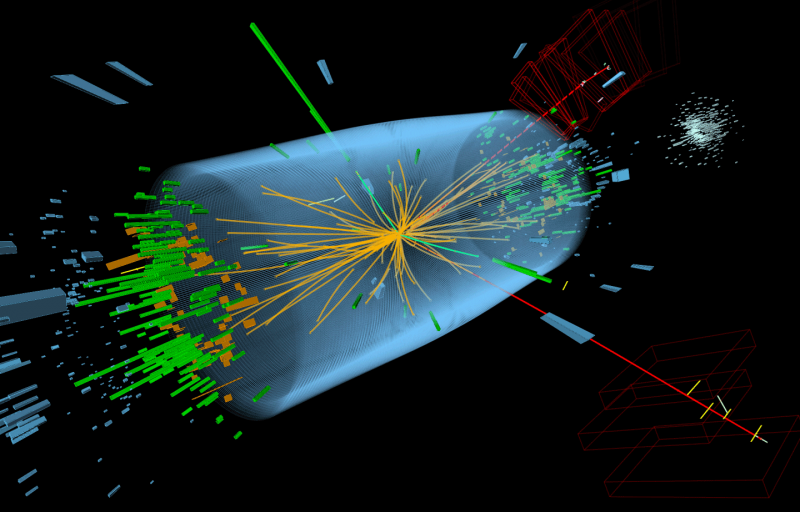
\includegraphics[scale=0.40]{particle_collision.png}
    \end{figure}
    \vfill
    Année académique 2019-2020
    \vfill
\end{center}

Ce document est une proposition de support de cours à destination des étudiants suivant le cours de physique subatomique, atomique et moléculaire. Il a été rédigé par les étudiants suivant ce même cours pendant l'année académique 2019-2020 et se base sur les slides mises à disposition par les professeurs, les notes de cours partagées par les étudiants ingénieurs (merci à Sofiane Arib et Pierre Laboureur) ainsi que diverses ressources externes (genre wikipédia tmtc).

\newpage
\tableofcontents

\newpage
\part{Introduction (Vincent Lemaître)}
\begin{center}
    En cas de questions ou de remarques sur cette partie : contactez Eléonore Lieffrig
\end{center}
\section{Introduction}
\subsection{Rappels sur les unités}
En physique atomique et subatomique, on n'utilisera pas les unités classiques que sont le \si{kg}, le \si{m}, etc., mais les unités naturelles, plus appropriées à l'échelle et aux dimensions des structures et phénomènes qui seront étudiés. L'unité de longueur est par exemple le femtomètre (\SI{e-15}{m}), ordre de grandeur du noyau atomique. De plus, on considérera, comme dans le système Heaviside-Lorentz, que  $\hbar=c=\epsilon_0=\mu_0=1$, ce qui transforme quelque peu des expressions familières comme celle de la constante de structure fine, qui devient

\[
    \alpha=\dfrac{e^2}{4\pi\epsilon_0\hbar c}=\dfrac{e^2}{4\pi}\approx\dfrac{1}{137}
\]
Une autre conséquence de cette hypothèse est illustrée dans le tableau ci-dessous: l'unité de masse, qui était précédemment une énergie par vitesse carrée,  devient une énergie, le \si{GeV} et celle de temps, quant à elle, devient l'inverse d'une énergie, le \si{GeV^{-1}}, avec $\SI{1}{GeV^{-1}}=\SI{6.59e-25}{s}$

\begin{table}[H]
    \centering
    \begin{tabu} to 0.7\textwidth {X[2.5,l]X[3.5,l]X[3,l]}
        \hspace*{-3.5mm} (a) & &\\
        \hline\hline
        Quantité & Unité dehaute énergie & Valeur en unité SI \\ \hline
        longueur & \SI{1}{fm} & \SI{e-15}{m} \\
        énergie  & $\SI{1}{GeV} = \SI{e9}{eV}$ & \SI{1.602e-10}{J} \\
        masse, $E/c^2$ & $\SI{1}{GeV}/c^2$ & \SI{1.78e-27}{kg}\\
        $\hbar = h/(2\pi)$ & \SI{6.588e-25}{GeV s} & \SI{1.055e-34}{J s}\\
        $c$ & \SI{2.998e23}{fm s^{-1}} & \SI{2.998e8}{ms^{-1}}\\
        $\hbar c$ & \SI{0.1975}{GeV fm} & \SI{3.162e-26}{J m}\\ \hline\hline \\
    \end{tabu}
    \begin{tabu} to 0.7\textwidth {XX}
        \hspace*{-3.5mm} (b) & \\
        \hline\hline
        \hspace*{-3mm} Unités naturelles; $\hbar = c = 1$ & \\
        masse, $Mc^2/c^2 $ & \SI{1}{GeV} \\
        longueur, $\hbar c/(Mc^2)$ & $\SI{1}{GeV^{-1}} = \SI{0.1975}{fm}$ \\
        temps, $\hbar c/(Mc^3)$ & $\SI{1}{GeV^{-1}} = \SI{6.59e-15}{s}$\\\hline
        \multicolumn{2}{l}{\hspace*{-3mm} Unités Lorentz-Heaviside, $\varepsilon_0 = \mu_0 = \hbar = c = 1$}\\
        constante de structure fine & $\alpha = e^2/(4\pi) \approx 1/137.06$\\\hline\hline
    \end{tabu}
    \caption{Unités naturelles}
    \label{tab:unites_naturelles}
\end{table}

\subsection{Tableau de Mendeleïev}
Le tableau de Mendeleïev (1869) représente tous les éléments chimiques, ordonnés par numéro atomique croissant et organisés en colonnes en fonction de leur configuration électronique, laquelle sous-tend leurs propriétés chimiques.  Le modèle de l'atome comportant des électrons sur des couches permet cette classification des éléments en familles, qui met en évidence la périodicité des propriétés chimiques. Par exemple, la première colonne est celle des Alcalins qui ne comportent qu'un seul électron sur la dernière couche et la dernière colonne est celle des Gaz nobles dont la dernière couche est fermée.

\begin{figure}[ht]
    \centering
    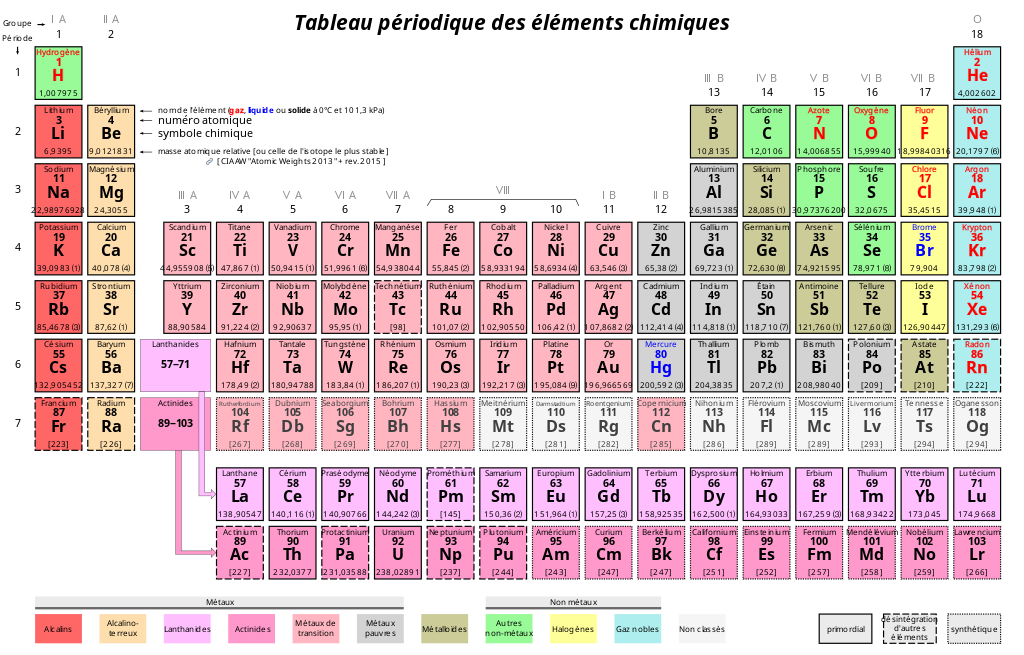
\includegraphics[scale=0.40]{Images1/mend.png}
    \caption{Tableau de Mendeleïev}
\end{figure}

Les atomes se situant dans la même période, c'est-à-dire dans la même ligne du tableau, possèdent le même nombre quantique principal n. Les éléments des mêmes groupes (i.e. même colonne) ont eux des configurations électroniques similaires et donc des propriétés chimiques similaires. On a différents groupes en fonction de la colonne: les métaux alcalins (1), les alcalino-terreux (2) ..., les halogènes (17), les gaz nobles (18). Enfin, les blocs sont des groupes d'éléments dont les électrons de valence occupent des orbitales qui partagent le même nombre quantique $l$ ($l=0,1, \dots, n-1$ correspondant à s, p, d,...).

Les éléments de ce tableau, les atomes, sont des objets très complexes dont la composition (pour le moment admise) est représentée ci-dessous, avec quelques ordres de grandeur. L'électron est un degré de liberté de l'atome, qui possède une charge et un spin, mais pas de position...

\begin{figure}[ht]
    \centering
    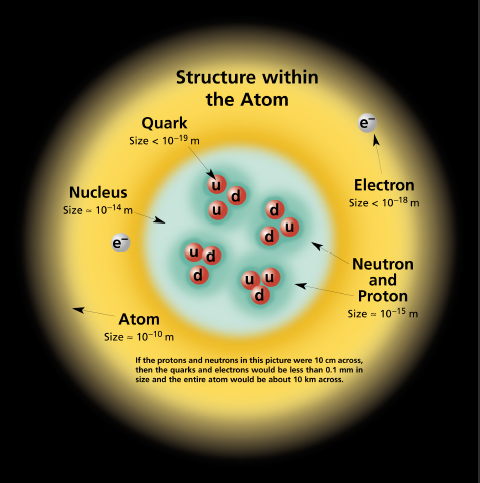
\includegraphics[scale=0.45]{Images1/atome.png}
    \caption{Structure de l'atome}
    \label{fig:struct_atome}
\end{figure}
On admet pour le moment que la matière est constituée de vide et des 4 particules suivantes:

\begin{itemize}
    \item \textbf{les quarks down}, possédant une charge électrique de -1/3
    \item \textbf{les quarks up}, possédant une charge électrique de 2/3
    \item \textbf{les électrons}, de charge -1, responsables des phénomènes électriques et des réactions chimiques
    \item \textbf{les photons}, responsables de l'interaction électromagnétique
\end{itemize}
Protons et neutrons sont composés de quarks: 1 down et 2 up pour le proton, 2 down et 1 up pour le neutron (logique).

\subsection{Modèles de la matière et liens avec la cosmologie et l'astrophysique}
La structure de la matière et l'interaction entre constituants sont intimement liées. En effet, c'est l'interaction entre les rayonnements et la matière qui autorise la description de la structure de celle-ci. Par exemple, les microscopes optiques permettent d'observer des objets de très petite taille, mais leur pouvoir de résolution (i.e leur capacité à séparer des détails très voisins) est limité par le caractère ondulatoire de la lumière, qui engendre de la diffraction. Ainsi, pour voir un objet de taille $d$, il faut un rayonnement dont la longueur d'onde associée $\lambda$ empêche la diffraction, c'est-à-dire telle que
\[ \lambda < d \]
La résolution limite pour de la lumière visible est donc de l'ordre de $\SI{0.5}{\mu m}$.

\subsubsection{Modèles de l'atome}
Différents modèles de plus en plus affinés se sont succédé pour décrire l'atome. Le modèle atomique du <<plum pudding>> fut proposé par J.J. Thomson (Fig \ref{fig:modele_thompson}), qui découvrit l'électron en 1897. Dans ce modèle, l'atome est composé d'électrons plongés dans une <<soupe>> de charges positives pour équilibrer cette charge positive, comme des prunes/raisins selon les versions dans un pudding. Les électrons ne se déplacent pas de façon aléatoire dans l'atome, mais sur des anneaux stabilisés par les interactions entre électrons.

\begin{figure}[ht]
    \centering
    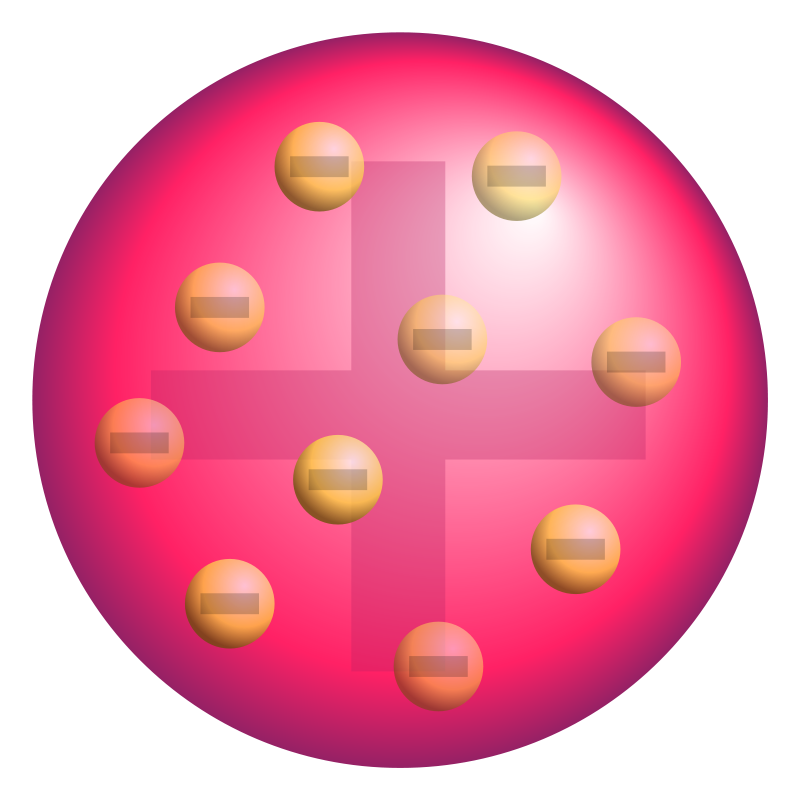
\includegraphics[scale=0.15]{Images1/thomson.png}
    \caption{Modèle de l'atome de Thomson (1897)}
    \label{fig:modele_thompson}
\end{figure}

Ernest Rutherford, considéré comme le père de la physique nucléaire, mit en évidence en 1909 l'existence du noyau atomique, ayant également prouvé au passage l'existence du proton. En 1932, Chadwick découvrit le neutron, remettant ainsi en question le modèle de l'atome. Rutherford imagine donc un atome constitué d'un noyau chargé positivement contenant la majorité de la masse de l'atome et, séparés par du vide, des électrons tournant autour de ce noyau comme des planètes autour d'une étoile (Fig \ref{fig:modele_rutherford}).

\begin{figure}[ht]
    \centering
    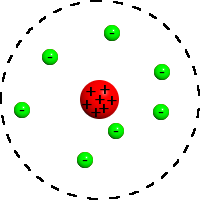
\includegraphics[scale=0.65]{Images1/modelerutherford.png}
    \caption{Modèle de l'atome de Rutherford (1909)}
    \label{fig:modele_rutherford}
\end{figure}

Les accélérateurs actuels (linéaires, circulaires (LHC)) nous permettent d'observer les plus petits constituants de la matière, mais plus la taille de ce que l'on souhaite observer est petite, plus ils doivent être grands, comme illustré ci-dessous. Sur les échelles suivantes sont également représentées les longueurs et énergies, liées par la relation de la longueur d'onde de de Broglie:
\[ \lambda=\dfrac{h}{\sqrt{2mE}} \]
En fait ici c'est un peu complexe, la vraie relation de la longueur d'onde de de Broglie c'est
\[\lambda=\dfrac{h}{p}\]
Ici la relation $p = \sqrt{2mE}$, vient de l'approximation non relativiste $E = \dfrac{p^{2}}{2m}$ (on voit déjà facilement que le cas purement relativiste de la lumière donne une longueur d'onde infinie). L'approximation reste malgré tout correcte assez longtemps (par exemple $v = c/10$ n'est pas du tout relativiste). Selon Lemaître la distinction de régime relativiste doit être faite lorsque l'énergie cinétique commence à être de l'ordre du terme de masse\footnote{Pour rappel, $E = E_\text{cin} + mc^2 = \gamma mc^2$}. Ce terme de masse dépend uniquement de la particule que l'on traite, pour un proton c'est $\SI{938}{MeV}/c^2$ , mais pour un muon c'est $\SI{105.66}{MeV}/c^2$ et un électron c'est 207 fois moins : $\SI{511}{keV}/c^2$. Donc, attention à la formule lorsqu'on dépasse \SI{100}{MeV} pour un proton.

\begin{figure}[ht]
    \centering
    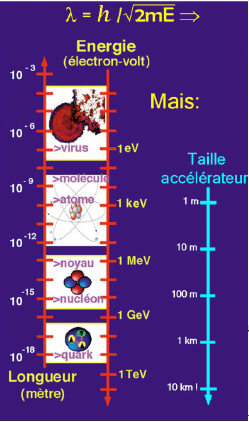
\includegraphics[scale=0.75]{Images1/echelles.png}
    \caption{Relation entre longueur et énergie}
    \label{fig:longeur_energie}
\end{figure}

\subsubsection{Connexion à la cosmologie}
Comprendre les interactions, c'est comprendre l'évolution, du Big Bang à l'apparition de la vie, soit faire de la cosmologie. La théorie du Big Bang de Lemaître et son hypothèse de l'atome primitif ont permis d'établir un lien entre l'infiniment petit (instant juste après le BB) et l'infiniment grand (l'Univers actuel).  Le rayonnement cosmique, la nucléosynthèse primordiale et l'expansion de l'Univers sont des éléments de preuve en faveur de cette théorie.

\begin{figure}[ht]
    \centering
    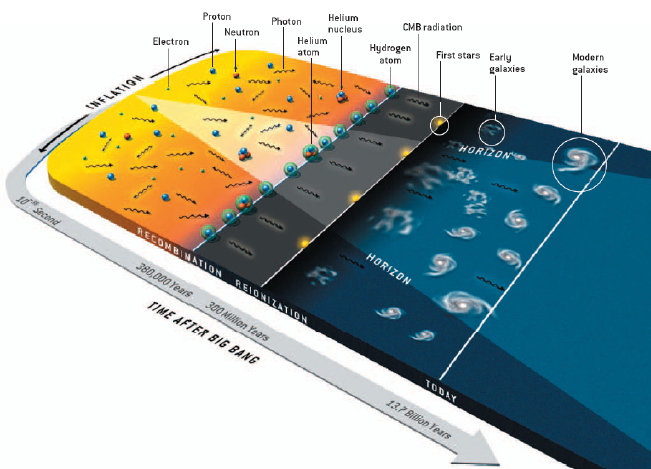
\includegraphics[scale=0.65]{Images1/univers.png}
    \caption{Évolution cosmique}
    \label{fig:evolution_cosmos}
\end{figure}

La ligne du temps de la figure \ref{fig:evolution_cosmos} représente l'évolution de l'Univers depuis le Big Bang. Pendant la première période, on est en présence d'un plasma chaud de gaz ionisé qui se refroidit petit à petit, au fur et à mesure que la nucléosynthèse primordiale se déroule. Elle s'est manifestée à l'échelle de l'Univers tout entier durant les premières dizaines de minutes suivant le Big Bang et est responsable de la formation des noyaux légers, principalement l'hélium 4, mais également le deutérium, une petite partie du lithium et des traces de béryllium. Aucun élément plus lourd n'a été créé durant cette période. Il y a juste déionisation de l'univers, car des atomes se forment.

On remarque ensuite une zone grise entre 380 000 ans et 300 000 millions d'années pendant laquelle l'Univers était <<éteint>>, c'est-à-dire neutre et opaque, il ne se passe rien à part les effets de la gravitation. Remarque: on ne sait pas encore vraiment comment se sont formés les éléments très lourds, car leur synthèse nécessite des conditions très particulières.

Après la période <<d'extinction>>, il y eut formation d'hydrogène et émission de lumière sous forme d'ondes radio, qui ont été détectées par des ingénieurs via des antennes en 1932. On note également le début de la formation des galaxies et des quasars.

Après 1 milliard d'années, l'Univers redevient <<transparent>>, la réionisation est complète,  beaucoup plus d'éléments du tableau périodique sont formés ; les galaxies évoluent. La réionisation a lieu, car les premières étoiles étaient très chaudes, à tel point qu'elles émettent dans l'UV, ce qui peut ioniser les atomes. On assiste à la formation du système solaire vers 9 milliards d'années.\\

On s'intéresse à présent aux premières minutes après le Big Bang au niveau des particules:
\begin{itemize}
    \item $t_0$: instant du Big Bang
    \item $t_0 + \SI{e-34}{s}$: compliqué, relève de la théorie des cordes et de la gravité quantique à boucles.
    \item $t_0 + \SI{e-12}{s}$: énergie de \SI{1}{TeV}, soupe de particules élémentaires (bosons W, quarks en tout genre, muons, positrons...). Il y a une légère asymétrie entre matière et antimatière, qui n'est toujours pas comprise à l'heure actuelle. Un peu après, il ne reste plus assez d'énergie pour créer une paire quark-antiquark, il reste donc quelques quarks tout seuls.
\end{itemize}

\begin{figure}[ht]
    \centering
    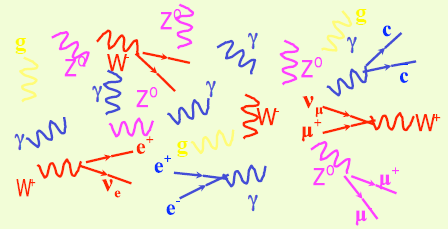
\includegraphics[width=0.45\textwidth]{Images1/soupe.png}
    \caption{Soupe primordiale}
    \label{fig:soupe_promordiale}
\end{figure}

\begin{rem}
    Comment peut-on affirmer avec certitude qu'il n'existe pas d'anti-monde rempli d'antimatière (une anti-galaxie avec un anti-soleil, etc.) ? Car il provoquerait des effets gravitationnels et électromagnétiques tellement cataclysmiques qu'on ne pourrait pas les rater.
\end{rem}

\begin{itemize}
    \item $t_0 + \SI{e-2}{s}$: énergie de \SI{1}{GeV}, mariage des quarks et formation des nucléons sous l'effet de l'interaction forte (neutron = 2 down + 1 up, proton = 2 up + 1 down)
    \item $t_0+ \SI{100}{s}$: \SI{100}{eV} ($10^9$ degrés), existence d'états liés entre neutrons et protons sous l'effet de l'interaction faible, comme le deutérium et l'hélium (noyaux légers).
\end{itemize}

\begin{figure}[ht]
    \centering
    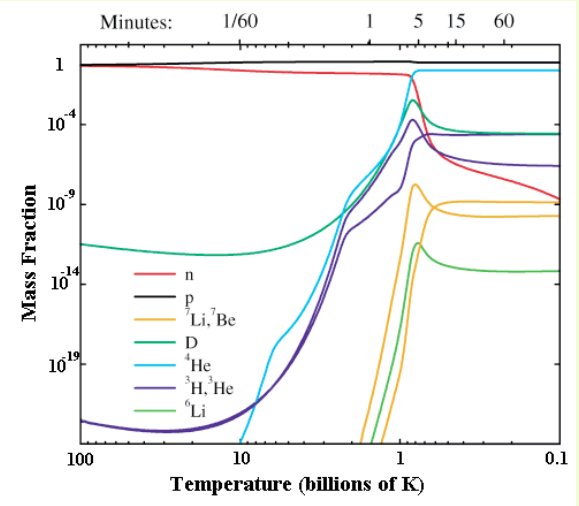
\includegraphics[scale=0.50]{Images1/tempmass.png}
    \caption{Évolution des proportions d'éléments en fonction du temps}
\end{figure}

\begin{itemize}
    \item $t_0+30$ min: le contenu de l'Univers est dominé par les protons et l'hélium (il y a aussi des électrons et photons). On est en présence d'un plasma électriquement neutre (Fig. \ref{fig:BB_30mn}).
    \item $t_0 + 300.000$ ans: les photons sont libres, on les observe
    \item $t_0 + 700.000$ ans: 3000 degrés, formation des atomes les plus simples sous l'effet de l'interaction électromagnétique
\end{itemize}

\begin{figure}[ht]
    \centering
    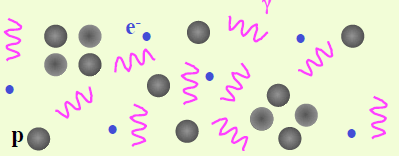
\includegraphics[scale=0.50]{Images1/30min.png}
    \caption{Univers 30 minutes après le Big Bang}
    \label{fig:BB_30mn}
\end{figure}

% \textcolor{blue}{[Revoir cette section]}
\subsubsection{Connexion à l'astrophysique}
En ce qui concerne la connexion à l'astrophysique, la structure microscopique de la matière permet une compréhension très riche des astres et du cosmos.

Par exemple le Nuage d'Orion est relativement proche de la Terre dans la Voie lactée. L'observation de son spectre permet de conclure sur sa composition en certains atomes et molécules. De telles conclusions ne seraient pas possibles sans la connaissance du monde microscopique pour décrypter ces observations.


\section{Structure de la matière}
Cette section porte sur la découverte de particules et de rayonnements, ainsi que sur leurs pertes d'énergie. Il est donc bon de commencer par restituer différents évènements sur une ligne du temps (Fig. \ref{fig:decouvertes}):

\begin{figure}[ht]
    \centering
    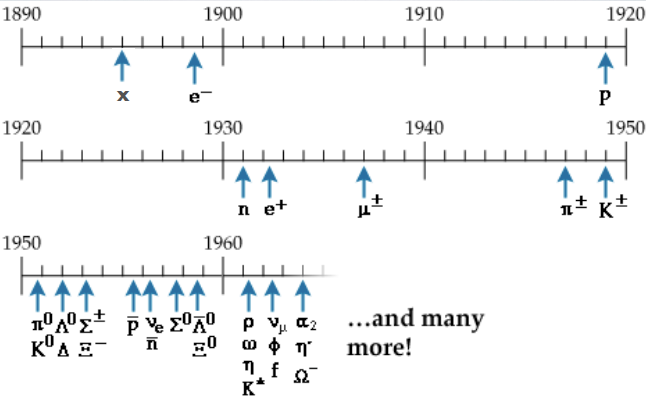
\includegraphics[scale=0.50]{Images1/ldt.png}
    \caption{Découverte de différentes particules et rayonnements}
    \label{fig:decouvertes}
\end{figure}

\begin{itemize}
    \item 1895: Découverte des rayons X (Roentgen)
    \item 1896: Découverte de la radioactivité (Becquerel)
    \item 1897: Découverte de l'électron (J.J. Thomson)
    \item 1909: Preuve que les particules $\alpha$ sont de noyaux d'hélium (Rutherford)
    \item 1911: Découverte du noyau (Rutherford)
    \item 1912: Découverte des rayonnements cosmiques (Hess)
    \item 1928: Théorie de l'$\alpha$-radioactivité (Gamow, Gurney, Condon)
    \item 1930: Hypothèse du neutrino (Pauli)
    \item 1932: Découverte du neutron (Chadwick)
    \item 1934: Théorie de la $\beta$-radioactivité (Fermi)
    \item ...
\end{itemize}


\subsection{Des rayons X à la découverte de l'électron}
\subsubsection{Fluorescence et phosphorescence}
Une molécule fluorescente possède la propriété d'absorber de l'énergie lumineuse (lumière d'excitation) et de la restituer rapidement sous forme de lumière fluorescente (lumière d'émission). Une fois l'énergie du photon absorbée, la molécule se trouve alors généralement dans un état électroniquement excité, souvent un état singulet, noté S1. (L'état fondamental qui est aussi singulet est noté S0.) Le retour à l'état fondamental peut alors se faire de différentes manières : soit par fluorescence, soit par phosphorescence (Fig. \ref{fig:fluorescence_phosphorescence}).

La fluorescence est caractérisée par l'émission d'un photon de manière très rapide. Cette rapidité s'explique par le fait que l'émission respecte une des règles de sélection de l'émission de photons de la mécanique quantique qui est $\Delta S=0$, ce qui signifie que la molécule reste dans un état singulet.

La phosphorescence quant à elle est caractérisée par une transition d'un état S=0 vers un état S=1 (état triplet noté T1), qui n'est pas permise par le modèle quantique, mais qui est rendue possible par le couplage spin-orbite. Cependant, la transition est plus lente à s'effectuer. Suit alors une émission de photon pour retourner à l'état fondamental.

\begin{figure}[ht]
    \centering
    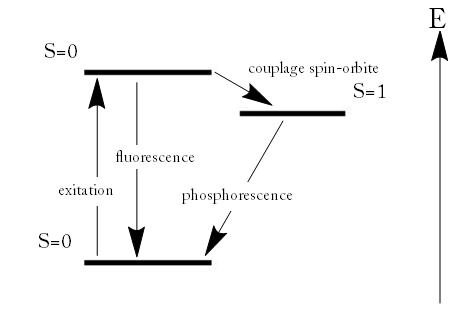
\includegraphics[scale=0.65]{Images1/fluophospho.jpg}
    \caption{Fluorescence VS phosphorescence}
    \label{fig:fluorescence_phosphorescence}
\end{figure}

\subsubsection{Découverte des rayons X (Röntgen, 1895, PN en 1901)}
Les rayons X sont une forme de rayonnement électromagnétique à haute fréquence constitué de photons. L'énergie de ces photons va d'une centaine d'$eV$ à environ un $\si{MeV}$. Anecdote: Röntgen les a appelés rayons <<X>> en référence à l'inconnue mathématique.

Ils sont de même nature que les rayons gamma, mais produits différemment : les rayons X sont produits par des transitions électroniques alors que les rayons gamma proviennent de la désintégration radioactive des noyaux des atomes.

Comment Röntgen les a-t-il découverts? Comme beaucoup de physiciens à l'époque, il se passionnait pour les <<rayons cathodiques>>, étudiés auparavant par William Crookes via les célèbres <<tubes de Crookes>>.

\begin{figure}[ht]
    \centering
    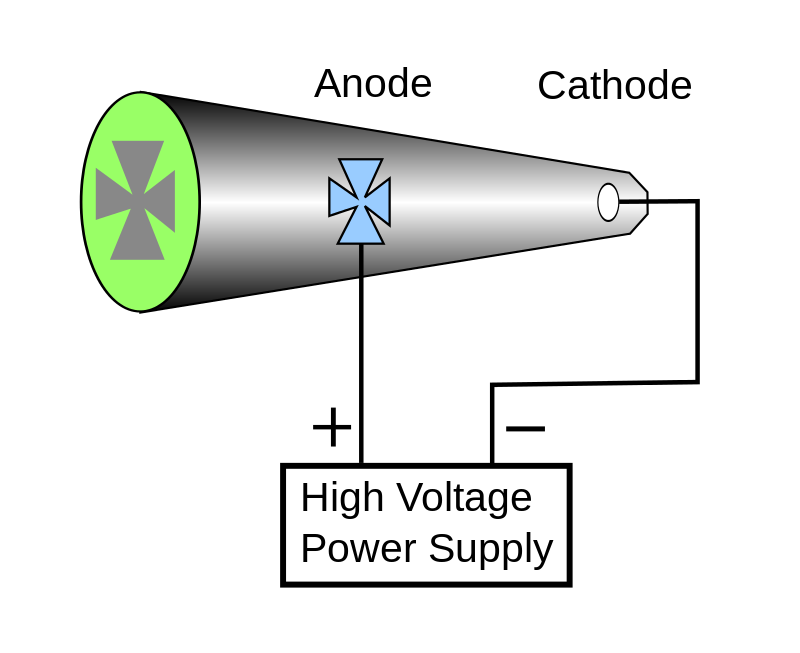
\includegraphics[scale=0.20]{Images1/tubecrookes.png}
    \caption{Schéma d'un tube de Crookes}
\end{figure}

Le tube de Crookes est un tube de verre froid sous vide partiel possédant 2 électrodes de métal, une à chaque extrémité. Quand on applique une forte tension électrique entre les électrodes, le champ électrique induit l'accélération des ions chargés présents dans le gaz résiduel. Ils entrent en collision avec les autres molécules du gaz, leur arrachant au passage des électrons, ce qui crée des cations. Ces derniers sont attirés par la cathode (électrode négative). À l'instant où ils la percutent, ils éjectent un grand nombre d'électrons de la surface métallique, qui sont eux attirés par l'électrode positive, l'anode. Ces électrons sont ce qu'on a appelé plus haut les <<rayons cathodiques>>. Il y a donc un faisceau d'électrons qui traverse le tube depuis la cathode vers l'anode.

Quand on applique une différence de potentiel supérieure ou égale à \SI{5 000}{V} à un tube de Crookes, les électrons sont accélérés à une vitesse telle qu'un rayonnement est émis de l'anode vers le récepteur. Le spectre de ce rayonnement est continu et comporte des pics. Il montre 2 caractéristiques témoignant de 2 phénomènes différents:

\begin{itemize}
    \item \textbf{Le rayonnement continu de freinage (ou Bremsstrahlung)} : les électrons accélérés émettent des rayons X au moment où ils passent à proximité de la charge électrique portée par le noyau atomique des molécules composant la cible et que leur trajectoire est brutalement infléchie. (car ils sont décéléré par le champ électrique des noyaux)
    \item \textbf{la fluorescence X} : quand les électrons rencontrent les <<électrons profonds>> d'un atome de la paroi du tube, ils les placent dans des niveaux d'énergie plus élevés, car ils leur arrachent des électrons sur la couche externe. Les électrons de l'atome doivent alors redescendre d'un niveau d'énergie pour se stabiliser, émettant au passage des rayons X.
\end{itemize}

En 1895, Röntgen manipulait un tube de Crookes recouvert d'un carton noir quand il s'aperçut qu'un des écrans scintillants situé à proximité du tube scintillait un peu. Il en déduit que les rayons issus du tube étaient capables de traverser le carton et faire fluorescer l'écran, même dans l'obscurité. Il observa aussi que les rayons traversaient ses livres et papiers, mais qu'il était plus ou moins pénétrant en fonction de la densité de l'objet à traverser. \\

Aujourd'hui, on produit les rayons X dans des tubes spéciaux (tubes à rayons X figure \ref{fig:tube_rayon_x}) qui sont en quelque sorte une évolution des tubes de Crookes. Contrairement à ces derniers, ils sont chauffés. Une haute tension est établie entre deux électrodes. Il se produit alors un courant d'électrons de la cathode vers l'anode comme expliqué plus haut. Les électrons sont freinés par les atomes de la cible, ce qui provoque un rayonnement continu de freinage ou Bremsstrahlung, dont une partie du spectre est dans le domaine des rayons X. Ces électrons excitent les atomes de la cible, et ceux-ci réémettent un rayonnement X caractéristique par le phénomène de fluorescence X. Le spectre sortant du tube est donc la superposition du rayonnement de freinage et de la fluorescence X de la cible (voir figure \ref{fig:spectre_rayon_x}). Le système représenté en bleu sur le schéma ci-dessous est un dispositif de circulation d'eau pour refroidie le tube, car la dissipation de chaleur est énorme, bien qu'aujourd'hui cet effet soit mieux contrôlé, notamment en faisant tourner l'anode pour qu'elle ne soit pas toujours percutée au même endroit. La bobine est souvent en tungstène.

\begin{figure}[ht]
    \centering
    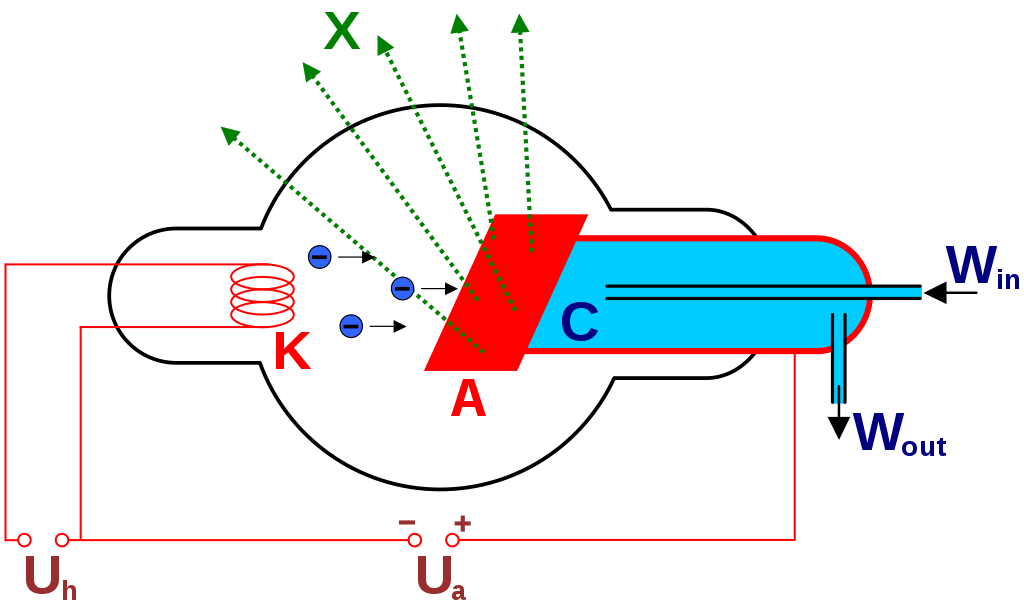
\includegraphics[width=0.5\textwidth]{Images1/rayonsxtube.png}
    \caption{Production de rayons X dans un tube à anode fixe}
    \label{fig:tube_rayon_x}
\end{figure}

\begin{figure}[ht]
    \centering
    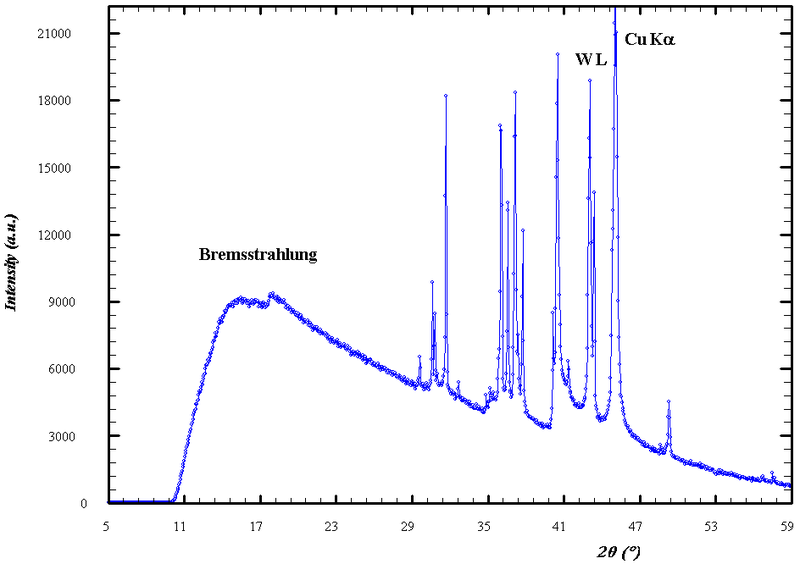
\includegraphics[scale=0.30]{Images1/rayonnement.PNG}
    \caption{Composition du spectre sortant du tube à rayons X}
    \label{fig:spectre_rayon_x}
\end{figure}

\subsubsection{Découverte de la radioactivité naturelle (Becquerel, 1896, PN en 1903)}
En 1896, Henri Becquerel cherche à déterminer si le phénomène de fluorescence des sels d'uranium est de même nature que les rayons X. Il dépose des sels phosphorescents d'uranium sur des plaques photographiques, elles-mêmes enveloppées dans du papier noir et les expose au soleil. Les photographies révèlent l'image des cristaux de sel d'uranium. Becquerel pense donc que l'énergie du soleil est absorbée par l'uranium avant d'être réémise sous forme de rayons X.

Cependant, un jour de mauvais temps, Becquerel doit renoncer à reproduire son expérience et il range donc ses plaques photographiques imprégnées de sels d'uranium dans un placard. Surprise, quelques jours plus tard, les plaques sont quand même impressionnées et Becquerel distingue même l'image négative d'une croix de cuivre qui se trouvait entre l'uranium et l'une de ses plaques photographiques. Il ne peut donc que conclure qu'une substance inerte se montre capable d'émettre des rayons, en l'absence de lumière, qui traversent le papier, mais sont tout de même arrêtés par le métal. \\

On a une loi de comportement pour décrire la désintégration radioactive: dans une boîte avec $N$ particules, le taux de désintégration ne change pas. C'est assez contre-intuitif par rapport à la nature, car si on fait une analogie avec notre classe, dans 50 ans, quelques-uns auront disparu à cause du vieillissement, mais ce nombre de disparus sera encore bien plus important dans 100 ans (rip). \textbf{Cette notion de vieillissement n'existe pas chez les particules}, elles se désintègrent au même taux à tout moment:
\[    \Delta N(t)=-\lambda N(t) \Delta t    \]
où
\begin{itemize}
    \item $N(t)$ est le nombre de noyaux radioactifs de l'espèce initiale existant à l'instant $t$. On suppose qu'il ne varie que très peu dans l'intervalle de temps $[t,t+\Delta t]$
    \item $\Delta N(t)$ est le nombre de noyaux qui se transforment pendant l'intervalle de temps $[t,t+\Delta t]$
    \item $\lambda$ est une constante de proportionnalité ayant les dimensions de l'inverse d'un temps, appelée constante radioactive (remarquons qu'elle ne dépend pas du temps: les atomes ne vieillissent pas)
\end{itemize}
On a donc
\[
    \fdif{N(t)}{t}=-\lambda N(t)
\]
ou encore
\[
    N(t)=N(0)e^{-\lambda t}
\]
N.B: une fois qu'ils ont découvert la radioactivité et ses <<pouvoirs curatifs miraculeux>>, les gens se sont un peu emballés...

\begin{figure}[H]
    \centering
    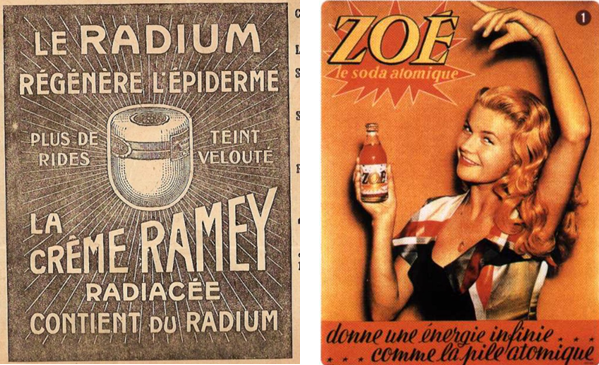
\includegraphics[scale=0.60]{Images1/produits.png}
    \caption{Crème et soda radioactifs}
\end{figure}

\subsubsection{Découverte de l'électron (Thomson, 1897, PN en 1906)}
Les tubes de Crookes furent utilisés dans de très nombreuses expériences afin de déterminer la nature des rayons cathodiques. Deux théories coexistaient : Crookes croyait qu'il s'agissait de <<corpuscules>> ou <<matière radiante>> c'est-à-dire d'atomes chargés électriquement. D'autres chercheurs pensaient qu'il s'agissait de vibrations de l'éther, une nouvelle forme de rayonnement électromagnétique. Le débat continua jusqu'à ce que J. J. Thomson mesure leur masse, prouvant qu'ils avaient affaire à des particules chargées négativement inconnues auparavant, qu'il appela <<corpuscules>>, mais qui furent plus tard appelées électrons. En 1869, on construisit une anode avec une forme de croix de Malte dans le tube. Lorsque le tube était allumé, il projetait une ombre en forme de croix sur la matière fluorescente dans la partie arrière du tube (figure \ref{fig:croix_de_malte}), montrant que les rayons se déplaçaient en ligne droite.

\begin{figure}[ht]
    \centering
    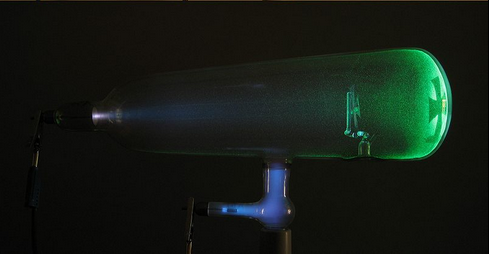
\includegraphics[scale=0.60]{Images1/croixmalte.PNG}
    \caption{Expérience de la croix de Malte}
    \label{fig:croix_de_malte}
\end{figure}

La preuve expérimentale de l'existence des électrons est le résultat de 3 expériences menées par Thomson:

\begin{itemize}
    \item Première expérience: Il cherche à savoir si on peut séparer la charge négative des rayons cathodiques par le biais du magnétisme. La conclusion est que ce n'est pas le cas. (d'où <<interprétation corpusculaire des rayons cathodiques>>)
    \item Deuxième expérience: Il prouve que les rayons cathodiques peuvent être déviés par un champ électrique. Il construit un tube cathodique muni d'une couche de peinture phosphorescente au bout pour détecter des rayons incidents. Thomson démontre une déviation dans un sens, qui indique que la charge des rayons cathodiques est négative. (Fig. \ref{fig:thompson_exp_2})

    \begin{figure}[ht]
        \centering
        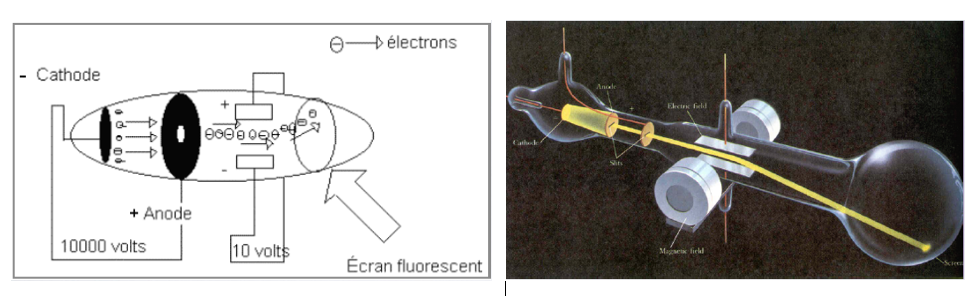
\includegraphics[scale=0.60]{Images1/2eexpthomson.PNG}
        \caption{Deuxième expérience de Thomson - Dispositif expérimental}
        \label{fig:thompson_exp_2}
    \end{figure}

    \item Troisième expérience: Détermination du rapport charge/masse $(e/m)$. Pour déterminer ce rapport, Thomson mesure la déviation et l'énergie cinétique des rayons cathodiques sous l'influence du champ magnétique. Son calcul lui donne un résultat pour $e/m$ mille fois plus élevé que le rapport analogue pour un ion hydrogène, ce qui suggère que les rayons cathodiques contiennent des particules soit très légères soit très hautement chargées. Thomson arrive à la conclusion que les rayons cathodiques sont composés de <<corpuscules>> qui proviennent de l'intérieur des atomes des électrodes, ce qui implique que les atomes sont divisibles. Le <<corpuscule>> découvert par Thomson est l'électron.
    S'en suit la proposition de modèle du <<plum pudding>> pour l'atome.
\end{itemize}

\subsubsection{Détermination de la charge de l'électron}
Elle se fit via l'expérience de la goutte d'huile de Millikan, qui consiste à pulvériser de minuscules gouttes d'huiles électrisées entre les 2 électrodes horizontales d'un condensateur plan chargé. Les gouttes sont soumises à plusieurs forces qui s'équilibrent rapidement, elles se déplacent donc à une vitesse constante qu'on peut mesurer.

\begin{figure}[ht]
    \centering
    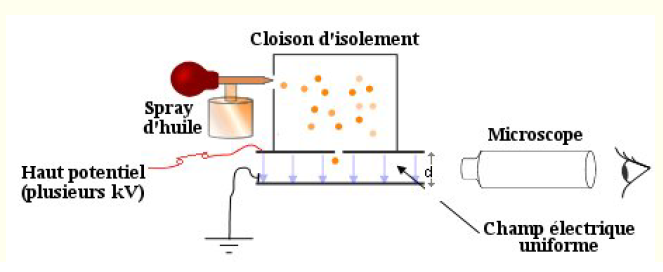
\includegraphics[scale=0.60]{Images1/millikan.PNG}
    \caption{Expérience de la goutte d'huile de Millikan}
\end{figure}

Le principe est de sélectionner une goutte, et  d'analyser son mouvement sous l'action des forces agissant sur elle  à différentes valeurs d'ionisation.

Millikan, mesura la vitesse d'une gouttelette d'huile qu'il ionisait en l'irradiant grâce à des rayons X. Cette mesure de la vitesse fut déterminée par le rapport entre la distance parcourue par la gouttelette d'huile et le temps mis pour effectuer ce déplacement. Ses observations lui firent se rendre compte que toutes les valeurs d'ionisation étaient multiples entiers de $e=\SI{1.592e-19}{C}$, que l'on définit comme la charge élémentaire.

\paragraph{Détails:} Si on modélise simplement le problème, la goutte d'huile subit les 4 forces suivantes:
\begin{itemize}
    \item Son poids $\Vec{P}=\dfrac{4}{3}\pi r^3 \rho_h\Vec{g}$
    \item La force électrostatique $\Vec{F_E}=q\Vec{E}$
    \item La poussée d'Archimède $\Vec{F_A}=-\dfrac{4}{3}\pi r^3 \rho_a \Vec{g}$
    \item La force de trainée (résistance de l'air) $\Vec{F_R}=-6\pi\eta r\Vec{v}$ où $\eta$ est le coefficient de viscosité de l'air et $v$ la vitesse de la gouttelette.
\end{itemize}
On peut mesurer la charge $q$ de la goutte de différentes façons. Considérons la méthode du champ constant, dans laquelle on garde l'amplitude du champ constante et on alterne la polarité du condensateur, de sorte que la force électrique soit dirigée tantôt vers le haut, tantôt vers le bas. \\[0,2cm]
Dans le cas de la force électrique vers le haut (vitesse $v_1$), on a
\begin{equation}
    qE+F_A = mg+6\pi\eta rv_1
    \label{eq:force_elec_haut}
\end{equation}
    Pour la force électrique vers le bas (vitesse $v_2$),
\begin{equation}
    qE+mg = 6\pi\eta rv_2 + F_A
    \label{eq:force_elec_bas}
\end{equation}
Si on soustrait (\ref{eq:force_elec_haut}) et (\ref{eq:force_elec_bas})
\[
    2(mg-F_A)=6\pi\eta r(v_2-v_1)
\]
vu que

\[
mg-F_A=\dfrac{4\pi}{3}r^3g(\rho_h-\rho_a)\quad\text{et}\quad
r=\dfrac{3}{2}\sqrt{\dfrac{\eta(v_2-v_1)}{g(\rho_h-\rho_a)}}
\]
Si on additionne (\ref{eq:force_elec_haut}) et (\ref{eq:force_elec_bas}), on obtient
\[
    2qE=6\pi\eta r(v_2+v_1)
\]
donc
\[
    q=\dfrac{9\pi}{2E}\sqrt{\dfrac{\eta^3(v_2-v_1)}{g(\rho_h-\rho_a)}}(v_2+v_1)
\]
Si on effectue 2 mesures de vitesse pour une goutte donnée, on peut donc déterminer $q$.

\subsection{Perte d'énergie dans la matière}

L'intérêt de l'étude de la perte d'énergie lors d'une interaction particule-matière réside dans le fait que c'est l'outil principal de détection de particule. Commençons par étudier la perte d'énergie des particules lourdes, c'est-à-dire des particules possédant une masse bien supérieure à celle de l'électron. Si elles ont une énergie basse, la perte d'énergie est dominée par leur interaction électromagnétique avec les électrons atomiques: il y a excitation et/ou ionisation de l'atome par transfert d'une partie de l'énergie cinétique de la particule incidente. Si au contraire elles ont une haute énergie, ce sont les interactions nucléaires qui sont importantes.

\subsubsection{Perte d'énergie par ionisation}
La section efficace (cfr section \ref{sec:section_efficace}) étant très petite (de l'ordre de \SI{e-17}{cm^2}), la probabilité de collision est très faible, mais la grande densité d'atomes ($N_A=\SI{6.02e23}{\mole^-1}$) dans un matériau rend la perte d'énergie totale très importante, même pour une faible épaisseur. Par exemple, un proton de 10 \si{MeV} perd toute son énergie dans \SI{0.25}{mm} de cuivre !

L'énergie est perdue par la particule dans des <<collisions inélastiques>> avec les électrons des atomes du matériau. On a un très grand nombre de collisions, par conséquent l'énergie perdue par collision est petite. On dit qu'on a affaire à une diminution \textbf{continue} d'énergie. À la fin du parcours, les électrons sont capturés par la particule jusqu'à ce que l'énergie de cette dernière soit de l'ordre de l'énergie thermique des atomes du milieu.

\begin{rem}
    Le phénomène est décrit à l'aide du terme collision, mais il n'y a pas nécessairement contact entre l'électron incident (ou la particule chargée) et l'électron de l'atome cible. Néanmoins, le phénomène résultant de cette interaction électrostatique de durée très brève peut s'apparenter à une collision.
\end{rem}

Calculons la perte d'énergie se faisant lors du passage à travers une couche $\dif x$ de matière, comme représenté sur la figure \ref{fig:interraction_particule_matiere}.
\begin{figure}[ht]
    \centering
    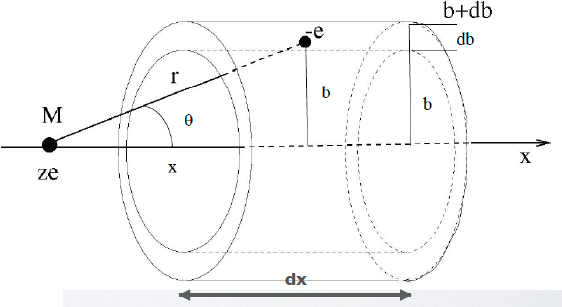
\includegraphics[scale=0.60]{Images1/pertenrj.PNG}
    \caption{Interaction entre particule (ze) et électron de matière}
    \label{fig:interraction_particule_matiere}
\end{figure}
L'impulsion verticale fournie par la particule incidente à un électron atomique à travers la force de Coulomb est
\[
    \Delta P_t=\int_{-\infty}^\infty F_y \dt=\int_{-\infty}^\infty \dfrac{ze^2}{4\pi \epsilon_0 r^2} \sin{\theta}\dfrac{\dif x}{v}
\]
où
\[\begin{cases}
    \dfrac{1}{r^2} &= \dfrac{\sin^2\theta}{b^2} \\[2mm]
    x &= \dfrac{b}{\tan{\theta}} \\[2mm]
    \dif x &= -\dfrac{b}{(\sin{\theta})^2}\dif\theta
\end{cases}\]
Ainsi
\[
    \Delta P_t=\int_{0}^\pi \dfrac{ze^2}{4\pi \epsilon_0}\dfrac{\sin{\theta}}{vb}\dif\theta = \dfrac{ze^2}{2\pi \epsilon_0 vb}
\]
Dans une approche non relativiste, l'énergie transmise à l'électron est
\[
    \dif E_E=\dfrac{p^2}{2m_e}=\dfrac{z^2e^4}{8\pi^2{\epsilon_0}^2v^2b^2m_e}
\]
En admettant une distribution uniforme des électrons, le nombre de <<collisions>> que la particule subit avec des électrons situés à un paramètre d'impact compris entre $b$ et $b+\dif b$ dans une épaisseur $\dif x$ est\footnote{$A$ est la masse molaire, $\dfrac{\rho N_A}{A}$ est donc le nombre d'atomes du milieu par unité de volume.}
\[
    \dif N_e=\dfrac{\rho N_A}{A}Z(2\pi b \dif b \dif x)
\]
qui engendre un transfert d'énergie
\[
    \dif T_e=\dif N_e\dif E_e=\dfrac{z^2e^4}{4\pi \epsilon_0^2v^2bm_e}\Big(\dfrac{\rho N_A}{A}\Big)Z \dif b \dif x
\]
Par unité de distance, on a donc la perte d'énergie
\[
    -\fdif{E}{x}=\int_{b_\text{min}}^{b_\text{max}} \fdif{T_e(b)}{x}=\Big(\dfrac{\rho N_A}{A}\Big)Z\dfrac{z^2e^4}{4\pi \epsilon_0^2m_ev^2}\ln{\Big(\dfrac{b_\text{max}}{b_\text{min}}\Big)}
\]
Cependant, on a un problème puisque cette intégrale diverge. On doit donc en limiter les bornes en utilisant des arguments qualitatifs à savoir les estimations de $b_\text{min}$ et $b_\text{max}$:

\begin{itemize}[label=$\rightarrow$]
    \item \underline{\textbf{b grand $\Leftrightarrow\Delta E(b)$ petit}}\\[0,2cm]
    Les électrons sont liés aux noyaux. Le transfert d'énergie est plus petit que l'énergie moyenne d'ionisation $I$ des électrons et le processus n'est plus efficace. On imposera donc que $\Delta E(b) > I$, ce qui donne
    \[
        \dif E_e=\dfrac{1}{(4\pi \epsilon_0)^2}.\dfrac{2z^2e^4}{b_\text{max}^2v^2m_e}=I
    \]
    \item \underline{\textbf{b petit $\Longleftrightarrow\Delta E(b)$ grand}}\\[0,2cm]
    L'énergie maximale transférable est
    \[
        \Delta E_\text{max}=T_{e,max}=\dfrac{2m_e\beta^2\gamma^2c^2}{1+\left(\dfrac{m_e}{m_0}\right)^2+2\cdot\dfrac{m_e\gamma}{m_0}}
    \]
    où $m_0$ est la masse de la particule incidente.
\end{itemize}
La perte d'énergie par ionisation est donc de la forme
\[
    \dfrac{1}{\rho}\fdif{E}{x} \sim K\dfrac{z^2}{\beta^2}\dfrac{Z}{A}  \ln{\left(\dfrac{T_\text{max}}{I}\right)}
\]

On peut détecter le dépôt d'énergie au moyen de techniques telles que l'émulsion photographique, la chambre à brouillards, la chambre à bulles, le scintillateur, la détection du rayonnement Cerenkov...
On peut voir dans la figure \ref{fig:perte_energie} et \ref{fig:pertes_ionisation} que la première partie de la courbe descend assez fort, la particule rayonne beaucoup.

\begin{figure}[ht]
    \centering
    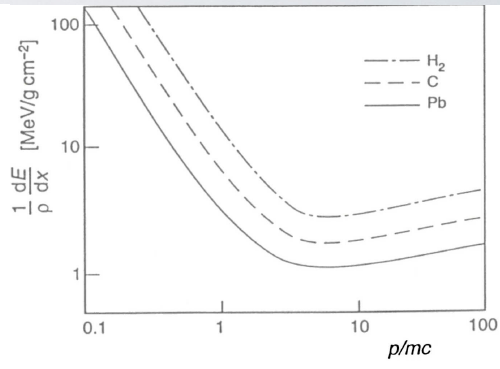
\includegraphics[scale=0.60]{Images1/perteenergie.PNG}
    \caption{Perte d'énergie par ionisation de quelques éléments}
    \label{fig:perte_energie}
\end{figure}

Un calcul plus précis, tenant compte des effets relativistes, et des corrections de densité de charge $\delta$ et $\dfrac{C}{Z}$, a été réalisé par Bethe et Block, et donne:
\[
    -\dfrac{1}{\rho}\fdif{E}{x} = K\dfrac{z^2}{\beta^2}\dfrac{Z}{A} \left[\ln\left(\dfrac{2m_ec^2\beta^2\gamma^2}{I}\right) - \beta^2-\dfrac{\delta}{2} -\dfrac{C}{Z}\right]
\]
où $K=\SI{0.307075}{MeV~g^{-1}~cm^2}$.

\begin{itemize}[label=$\longrightarrow$]
    \item \textbf{La correction de densité de charge} $\delta$ est due au fait que le champ électrique de la particule incidente polarise les atomes près de sa trajectoire. Cette polarisation réduit l'effet du champ électrique sur les électrons les plus éloignés (effet d'écran). Cela réduit la perte d'énergie. Cet effet est plus important si l'énergie des particules augmente (car le champ électrique est plus étendu), ou si la densité du matériau est plus élevée.
    \item \textbf{La correction $\dfrac{C}{Z}$} tient compte des effets de liaison des électrons et est importante à basse énergie.
\end{itemize}

\begin{rem}
    Cette formule met bien en évidence les dépendances de $\fdif{E}{x}$: le terme en $\dfrac{z^2}{\beta^2}$ montre la dépendance en la particule incidente (exemple: une particule $\alpha$ perd 4 fois plus d'énergie qu'un proton, pour un même $\beta$ et un même milieu), et celui en $\dfrac{Z}{A}$ montre la dépendance du milieu.
\end{rem}
\begin{rem}
    La relation entre $\fdif{E}{x}$ et la profondeur de pénétration est appelée courbe de Bragg. La dépendance en $1/v^2$ est marquée par la présence d'un pic appelé pic de Bragg (Figure \ref{fig:pic_bragg}). Cette caractéristique est utilisée en physique médicale dans le traitement de certaines tumeurs (on s'arrange pour que le pic de Bragg arrive pile à l'endroit de la tumeur et lui délivre donc toute son énergie).
\end{rem}

\begin{figure}[H]
    \centering
    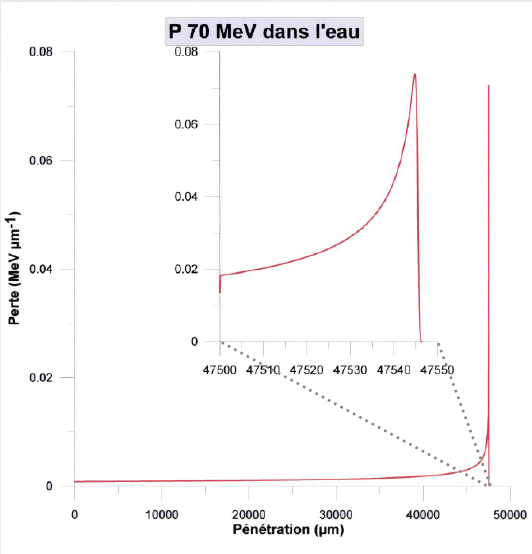
\includegraphics[width=0.5\textwidth]{Images1/picbragg.PNG}
    \caption{Courbe de Bragg théorique pour des protons de 70 \si{MeV} dans l'eau}
    \label{fig:pic_bragg}
\end{figure}

\begin{figure}[H]
    \centering
    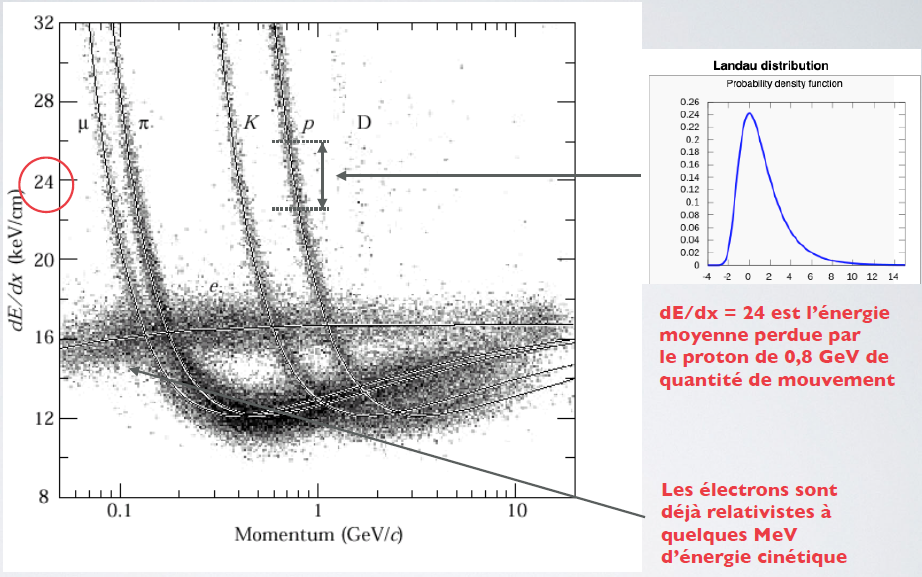
\includegraphics[width=0.66\textwidth]{Images1/perteionisation.PNG}
    \caption{Perte d'énergie par ionisation}
    \label{fig:pertes_ionisation}
\end{figure}

\subsubsection{Perte d'énergie par radiation}
À très haute énergie, les pertes d'énergie par collision deviennent négligeables par rapport aux pertes par radiation. Cet effet n'est important que pour les particules légères.

\begin{figure}[ht]
    \centering
    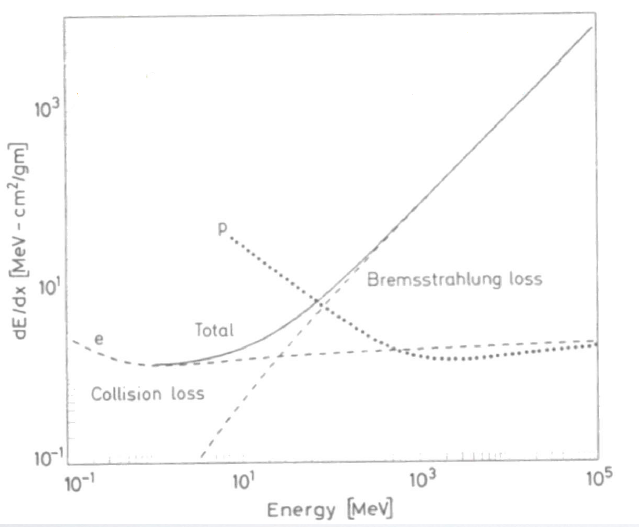
\includegraphics[scale=0.40]{Images1/bremstrucmachin.png}
    \caption{Pertes par collision et par radiation pour des électrons dans du cuivre}
    \label{fig:pertes_collision}
\end{figure}

La courbe qui monte linéairement (attention : graphe logarithmique) en pointillés est le Bremsstrahlung, le rayonnement de freinage qui correspond à l'interaction avec les noyaux n'ayant lieu qu'à hautes énergies, ce qui correspond également au domaine de valeur où la perte par ionisation ou collision (avec les e- des particules cibles) est négligeable. La courbe de cette interaction représentée en pointillés également et est plus ou moins plate, mais remonte à gauche, la zone où elle est prépondérante n'est en fait pas représenté sur le schéma. Le graphe montre également le comportement d'un proton qui réagit donc de manière opposée lors de ces interactions.\\
On constate que quand l'électron devient relativiste ($E>>m$), le rayonnement de freinage (Bremsstrahlung) domine rapidement. Les électrons perdent donc leur énergie par collision sur les électrons du milieu (Möller) et par diffusion élastique sur les noyaux (Mott): il y a déviation de leur trajectoire initiale et rayonnement de freinage. Le rayonnement de freinage varie en $Z^2$ de la cible.

\begin{figure}[ht]
    \centering
    \begin{subfigure}{.5\textwidth}
        \raggedright
        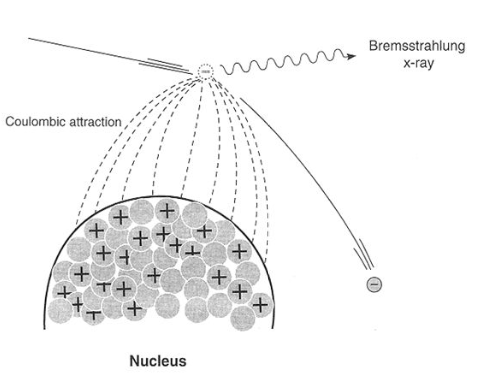
\includegraphics[width=.9\linewidth]{Images1/Bremsstrahlung2.PNG}
        %\caption{A subfigure}
        %\label{fig:sub1}
    \end{subfigure}%
    \begin{subfigure}{.5\textwidth}
        \raggedleft
        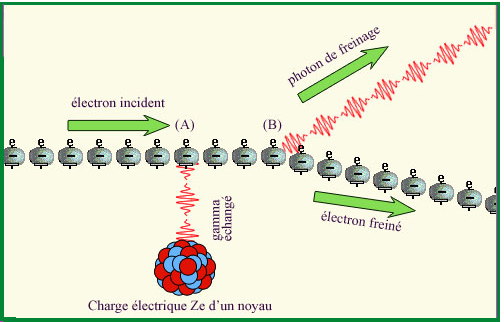
\includegraphics[width=.9\linewidth]{Images1/Bremsstrahlung3.PNG}
        %\caption{A subfigure}
        %\label{fig:sub2}
    \end{subfigure}
    \caption{Mécanisme du rayonnement de freinage}
    \label{fig:rayonnement_freinage}
\end{figure}

\paragraph{Notes supplémentaires sur le Bremsstrahlung:} Le phénomène de rayonnement de freinage (Fig. \ref{fig:rayonnement_freinage}) (Bremsstrahlung en allemand) concerne des particules porteuses d’une charge électrique dont la vitesse est proche de la vitesse de la lumière. Il intervient quand cette particule ultrarelativiste interagit avec un fort champ électrique ou magnétique, qui peut être naturel (le champ électrique d’un noyau) ou produit par l’homme (le champ d’aimants dans un accélérateur de particules). Les électrons et positons qui atteignent facilement des vitesses proches de celle de la lumière du fait de leur très faible masse sont les premiers concernés par le phénomène. \\

Le rayonnement de freinage intervient peu dans le domaine de la radioactivité, les électrons des désintégrations bêta n'étant souvent pas assez énergiques. Par contre, il joue un rôle important dans le rayonnement cosmique et le fonctionnement des accélérateurs de particules. \\

Sous l’effet de l’interaction, l’électron ou le positon, émets un photon qui emporte une partie de son énergie. L’électron est freiné et sa trajectoire modifiée. Le rayonnement de freinage est à l’origine d’une déperdition d’énergie dans de grands accélérateurs de particules comme les collisionneurs où les particules sont soumises à l’action de puissants aimants qui courbent leur trajectoire. Les ingénieurs des accélérateurs doivent compenser en permanence cette déperdition.

\subsubsection{Perte d'énergie des photons}
\begin{figure}[ht]
    \centering
    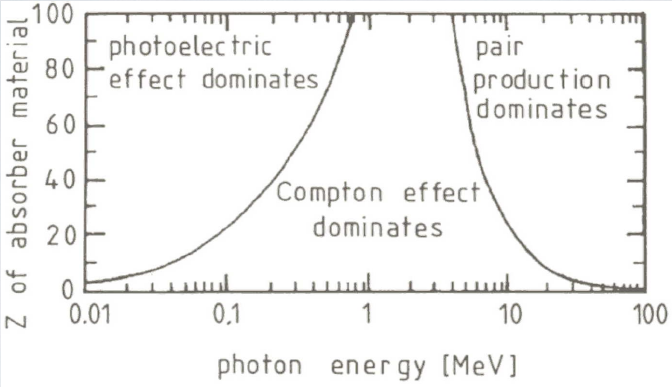
\includegraphics[scale=0.60]{Images1/pertephotons.PNG}
    \caption{Perte d'énergie des photons dans la matière}
    \label{fig:pertes_energie_photos}
\end{figure}
On constate bien sur la figure \ref{fig:pertes_energie_photos} que l'effet Compton est en compétition avec l'effet photoélectrique et la production de paires dans la perte d'énergie par les photons dans la matière\\

La diffusion Compton correspond à la collision d’un photon et d’un électron : le photon rebondit sur un électron cible qui est mis en mouvement et perd de l’énergie. L'électron est arraché à la matière, qui est donc ionisée, et le photon est diffusé. L'effet Compton contribue à l'atténuation des rayons gammas.  Arthur Compton a, en 1923, observé l'allongement de la longueur d'onde du photon dans cette diffusion, effet auquel on a attribué son nom : l'effet Compton.

\begin{figure}[ht]
    \centering
    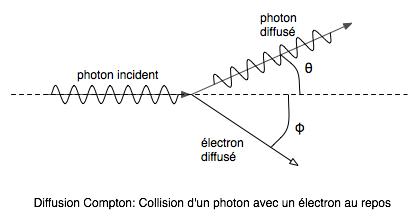
\includegraphics[scale=0.60]{Images1/compton.png}
    \caption{Diffusion Compton}
\end{figure}

La longueur d'onde change selon la formule
\[
    \lambda_f-\lambda_i=\dfrac{h}{m_ec}(1-\cos{\theta})
\]

\subsection{Découverte des rayonnements $\alpha$, $\beta$, $\gamma$}
\subsubsection{Radioactivité}
La radioactivité est le phénomène physique selon lequel des noyaux atomiques instables se transforment spontanément en d'autres atomes (désintégration) en émettant simultanément des particules de matière (électrons, noyaux d'hélium, neutrons, etc.) et de l'énergie (photons et énergie cinétique). Elle a été découverte en 1896 par Henri Becquerel dans le cas de l'uranium, et très vite confirmée par Marie Curie pour le radium. \\

Becquerel étudie le phénomène de phosphorescence. On connaissait déjà ce phénomène via lequel des matériaux émettent de la lumière dans le noir après avoir été exposés à la lumière (éventuellement des rayons X, découverts peu avant). Or, comme expliqué ci-dessus, Becquerel constata le noircissement des émulsions même en l'absence d'exposition à la lumière de sels d'uranium. Il y a donc des substances naturellement radioactives. Serait-ce donc une nouvelle émission similaire aux rayons X ? Quand on met ces substances naturellement radioactives dans une boîte blindée percée d'un petit trou, on observe 3 types de rayonnements: <<positif>>, <<neutre>>, et <<négatif>>, respectivement les rayonnements $\beta$, $\gamma$ et $\alpha$ (Fig. \ref{fig:alpha_beta_gamma}). Ils sont plus ou moins pénétrants dans la matière.

\begin{figure}[ht]
    \centering
    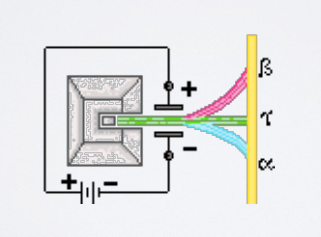
\includegraphics[width=0.4\textwidth]{Images1/rayonnements.PNG}
    \caption{Rayonnements $\alpha$, $\beta$, $\gamma$}
    \label{fig:alpha_beta_gamma}
\end{figure}

\begin{itemize}
    \item \textbf{Rayonnements $\alpha$}: Très vite arrêté par la matière (après une feuille de papier), spectre en énergie sous forme de raies dépendant de l'élément, produits par désintégration $\alpha$. C'est la forme de désintégration radioactive où un noyau atomique X éjecte une particule alpha (forme de rayonnement émis par des noyaux instables de grande masse atomique constitué de deux protons et deux neutrons combinés en une particule identique au noyau d'hélium 4 (hélion)) et se transforme en un noyau Y  de nombre de masse diminué de 4 et de numéro atomique diminué de 2. \\
    Forme générale:
    \[
        ^{A}_{Z}X \longrightarrow ^{A-4}_{Z-2}Y + ^{4}_{2} He ~ (+Q)
    \]
    Exemple:
    \[
        ^{238}U \longrightarrow ^{234}Th + \alpha
    \]
    Bilan énergétique d'une désintégration $\alpha$:
    \[
        Q = T_Y + T_\alpha = [M_{at}(X)-M_{at}(Y)-M_{at}(He)]c^2>0
    \]
    \[
        Q=B(A-4,Z-2)+B(^{4}_{2}He)-B(A,Z)>0
    \]

    \item \textbf{Rayonnements $\beta$}: La radioactivité bêta ou émission bêta est un type de désintégration radioactive dans laquelle une particule bêta (un électron ou un positon) est émise. Aujourd'hui, la désintégration $\beta$ se généralise à toutes les réactions nucléaires impliquant les neutrinos ou antineutrinos. Elle possède un plus grand pouvoir de pénétration (quelques millimètres), et est difficile à observer. Son spectre d'énergie est continu.

    Dans le cas du rayonnement $\beta$, si on trace le graphe de l'énergie des particules (Fig \ref{fig:spectre_beta}), on observe que la conservation de l'énergie n'est pas respectée. C'est ce constat qui inspira l'hypothèse de l'existence du neutrino.

    \begin{figure}[ht]
        \centering
        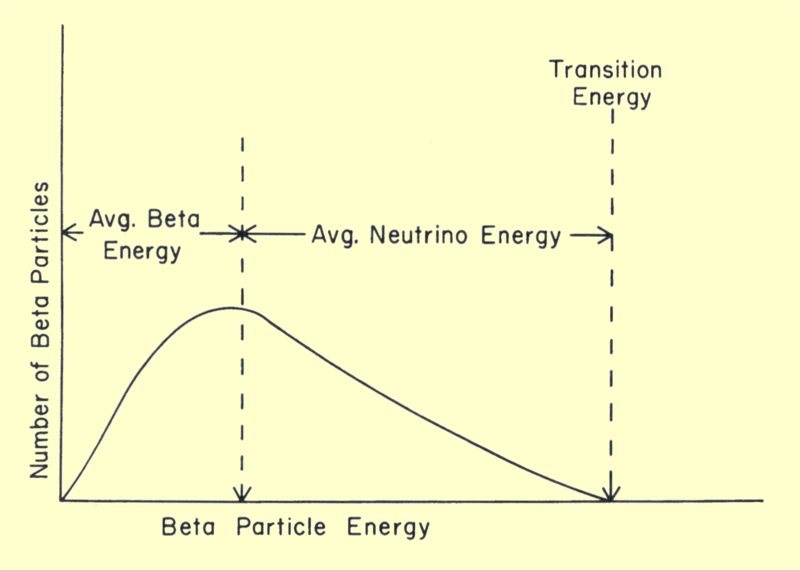
\includegraphics[scale=0.25]{Images1/beta.png}
        \caption{Spectre en énergie de la particule $\beta$}
        \label{fig:spectre_beta}
    \end{figure}

    On parle de désintégration bêta moins ($\beta^{-}$) ou bêta plus ($\beta^{+}$) selon qu'il s'agit de l'émission d'un électron ou d'un positon. Dès lors, on a respectivement les désintégrations suivantes :

    Forme générale:

    \[
        ^{A}_{Z}X \longrightarrow ^{A}_{Z+1}Y + e^- + \bar{\nu}_e
    \]

    \[
        ^{A}_{Z}X \longrightarrow ^{A}_{Z-1}Y + e^+ + \nu_e
    \]

    Exemple:
    \[
        ^{60}_{}Co \longrightarrow ^{60}_{}Ni^{+} + e^- + \bar{\nu}_e
    \]

    \[
        ^{18}_{}F \longrightarrow ^{18}_{}O + e^+ + \nu_e
    \]

    Il peut être intéressant de préciser que l'effet final d'un rayonnement Beta, pour un noyau radioactif instable, est de stabiliser le noyau (rétablir une balance n/p) en convertissant un neutron en proton et inversement (donc en émettant un e$^+$ ou e$^-$).

    \item \textbf{Rayonnements $\gamma$:} Possèdent un pouvoir de pénétration supérieur aux rayonnements alpha et beta et rayons X (ils passent quelques centimètres de plombs), spectre énergétique sous forme de raies. Le mécanisme de production des rayons $\gamma$ est illustré à la figure \ref{fig:rayons_gamma}.
\end{itemize}
\begin{figure}[ht]
    \centering
    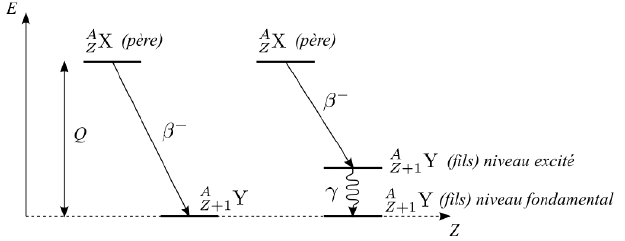
\includegraphics[width=0.8\textwidth]{Images1/gamma.PNG}
    \caption{Rayonnement $\gamma$}
    \label{fig:rayons_gamma}
\end{figure}
Les différents rayonnements obéissent à la loi de désintégration. Leur absorption est également exponentielle:
\[
    I(d)=I_0e^{-\mu d}
\]
où $\mu$ est un coefficient d'absorption\footnote{Ouais il a juste repris de Wikipédia. C'est quand ils passent dans la matière, ils sont absorbés de manière exponentielle et le mu dépend du matériau.}.


\section{Structure du noyau}
\subsection{Concept de section efficace}\label{sec:section_efficace}
\subsubsection{Définition}
Le concept de section efficace (Fig. \ref{fig:section_efficace}) couramment utilisé en physique nucléaire. C'est une grandeur physique reliée à la probabilité d'interaction d'une particule pour une réaction donnée. Son unité est le barn ($1b=10^{-24}cm^2$).
Quand on envoie un faisceau de particules, qu'on assimile à des sphères dures sur une cible, la probabilité d'interaction avec celle-ci est
\[
    \delta P_{int}=\dfrac{\text{Surface des sphères projetées}}{\text{Surface totale}}=\delta N \dfrac{\pi r^2}{S}=n \dif x \pi r^2
\]
où
\begin{itemize}
    \item $\delta N$ est le nombre de boules vues pour une surface S
    \item n est la densité volumique de sphères
    \item $\dif x$ est l'épaisseur de la cible
    \item $\sigma=\pi r^2$ est la section efficace géométrique
\end{itemize}

\begin{figure}[ht]
    \centering
    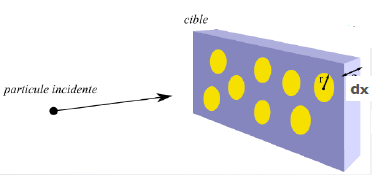
\includegraphics[scale=0.75]{Images1/section_efficace.PNG}
    \caption{Concept de section efficace}
    \label{fig:section_efficace}
\end{figure}
Si on a $N_i$ particules incidentes et $\dif N$ interactions pour une cible d'épaisseur $\dif x$, on admet comme définition de $\sigma$
\[
    \dif N=-N_in\sigma \dif x
\]
La section efficace ne dépend que du projectile et de la cible élémentaire. Pour une section efficace géométrique de l'ordre de \SI{100}{mb}, on a $r_o=\sqrt{\dfrac{\sigma}{\pi}}\sim \SI{e-15}{m} = \SI{1}{fm}$, ce qui est la taille typique des nucléons. Cela explique que, $\sigma(p+\text{noyau})\propto A^{2/3}$ car rayon du noyau $\propto A^{1/3}$.

\subsubsection{Section efficace d'interaction et temps de vie}
On considère une cible de surface S sur laquelle sont projetées des particules pendant une expérience. La section efficace pour cette réaction est $\sigma$. Si $n_0$ est le nombre de noyaux cibles par \si{cm^3}, alors le nombre total de noyaux cibles est $n_0 V$ = $n_0 S x$ et la section efficace de toutes les cibles est $\sigma_{tot}$ = $\sigma n_0 S X$. On peut donc déduire la probabilité qu'il y ait une réaction:
\[
    P=\dfrac{\sigma_{tot}}{S}
\]
et, sachant que $I$ est le nombre de particules incidentes durant toute l'expérience, le nombre de réactions durant l'expérience
\[
    N=I \sigma n_0 x
\]
Définissons maintenant la section efficace en tenant compte des composantes angulaires lors de la diffusion de la particule (Fig. \ref{fig:diffusion_particule}).

\begin{figure}[ht]
    \centering
    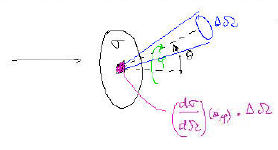
\includegraphics[scale=0.95]{Images1/secdiff.PNG}
    \caption{Représentation de la diffusion d'une particule}
    \label{fig:diffusion_particule}
\end{figure}
\noindent La section efficace telle que la particule part dans l'angle solide $\Delta\Omega$ centré sur $\theta$, $\phi$ est
\[
    \sigma=\int_{4\pi}^{}\fdif{\sigma}{\Omega}\dif \Omega
\]
où $\fdif{\sigma}{\Omega}$ est la section efficace différentielle. On a donc pour le nombre de réactions durant l'expérience
\[
    \dif N=I~n_0~X~\Big(\fdif{\sigma}{\Omega}\Big)~\Delta\Omega \quad\text{avec}\quad \fdif{\sigma}{\Omega}=\dfrac{\dif\sigma}{\dif\phi \dif \;(\cos{\theta})}=\dfrac{1}{2\pi}\fdif{\sigma}{\;(\cos{\theta})}
\]
Pour se représenter la situation, le détecteur correspond à un anneau réalisant toute une révolution autour de l'axe de l'expérience avec un avec $\phi$ (la direction de propagation des particules incidentes) et cela à un certain angle $\theta$.

\subsubsection{Longueur d'atténuation}
On a $\dif N=I_0 n_0 \sigma \dif x=-\dif I$. Si on intègre, on obtient
\[
    \int_{I_{0}}^{I(x)}\dfrac{\dif I}{I}=-\int_0^x n_0.\sigma \dif x
\]
c'est-à-dire que
\[
    I(x)=I_0e^{-n_0.\sigma.x}=I_0.e^{-x/x_0}
\]
On définit $x_0=\dfrac{1}{n_0\sigma}$ comme la longueur d'atténuation.

\subsubsection{Section efficace différentielle}
La section efficace (et donc la probabilité d'interaction) dépend de paramètres géométriques tels que le flux de particules uniforme dans le plan perpendiculaire à la direction de propagation $\Phi=\dfrac{\dif^2N}{\dif t\dif s}$, le nombre de particules diffusées par unité de temps et par unité d'angle solide dans la direction $(\theta, \theta+\dif \theta)$.
\begin{figure}[ht]
    \centering
    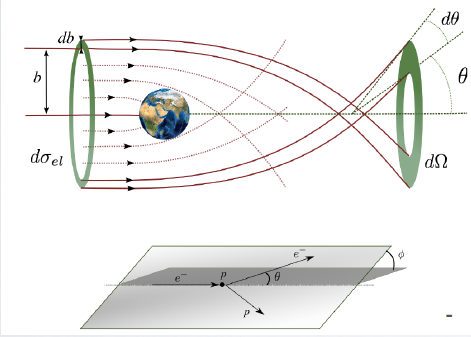
\includegraphics[scale=0.75]{Images1/section_efficace_diff.PNG}
    \caption{Concept de section efficace différentielle}
    \label{fig:section_efficace_diff}
\end{figure}
On a
\[
    \dfrac{\dif^2N}{\dif t\dif \Omega}=\dfrac{\dif^2N}{\dif t\dif \sigma_{el}} \fdif{\sigma_{el}}{\Omega}
\]
Si on mesure le nombre d'électrons à $\theta$ fixé,
\[
    \fdif{\sigma_{el}}{\Omega}=\dfrac{2\pi~b~\dif b}{2\pi \sin{\theta}\dif \theta}
\]
et à angle solide fixé,
\[
    \dif N=N_i~n~\dif x~\dif \Omega~\fdif{\sigma}{\Omega}
\]

\begin{figure}[ht]
    \centering
    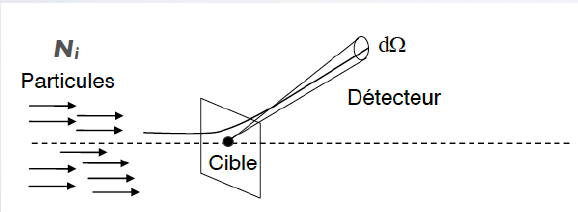
\includegraphics[scale=0.75]{Images1/anglesolide.PNG}
    \caption{Angle solide fixé}
\end{figure}
Remarquons que
\[
    \int(\fdif{\sigma}{\Omega})\dif \Omega=\sigma_{tot}
\]
Du fait de la symétrie, toutes les particules qui ont des paramètres d'impact compris entre $b$ et $b+\dif b$ seront diffusées entre $\theta$ et $\theta+\dif\theta$. Elles sont donc associées à une <<surface>> $2\pi b\cdot \dif b$ perpendiculaire au faisceau (figure \ref{fig:surface_de_diffusion}).
\begin{figure}[ht]
    \centering
    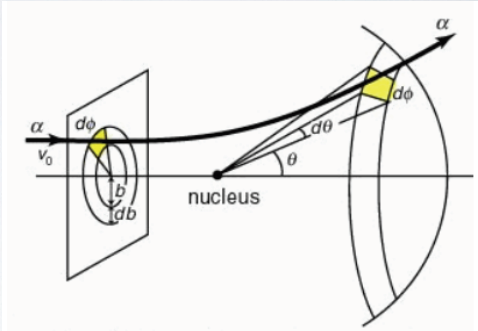
\includegraphics[scale=0.75]{Images1/surface_perp.PNG}
    \caption{<<Surface de diffusion>>}
    \label{fig:surface_de_diffusion}
\end{figure}
Pour une épaisseur x
\[
    \dif N=N_i~n_{\text{cible}}~x~\left(\fdif{\sigma}{\Omega}\right)\dif \Omega
\]
Si on intègre sur l'angle phi, on obtient la définition de \textbf{section efficace différentielle}
\[
    \fdif{\sigma}{\Omega}=\dfrac{2\pi b \dif b}{\dif \Omega}=\dfrac{2\pi~b~\dif b}{2\pi \sin{\theta}\dif\theta}=\dfrac{b}{\sin{\theta}}\abs{\fdif{b}{\theta}}
\]

\subsubsection{Section efficace de Rutherford}
Le développement est très bien expliqué sur \url{http://res-nlp.univ-lemans.fr/NLP_C_M13_G01/co/Contenu17.html}. L'auteur ne fait pas tout à fait comme Lemaître, mais arrive au même résultat.

\subsubsection{Expérience de Geiger et Marsden}
Cette expérience montra que la partie chargée positivement de la matière est concentrée en un espace de petit volume, le noyau atomique. L'expérience est réalisée sous vide. De la matière radioactive émettant des particules $\alpha$ est placée dans une boîte et le faisceau de particules $\alpha$ est orienté en direction d'une très fine feuille d'or (6 000 $\angstrom$). Derrière cette couche d'or, un écran est placé ; il est enrichi d'une substance chimique permettant de visualiser, par un scintillement lumineux, la collision par les particules $\alpha$ (Fig. \ref{fig:geiger_marsden}).

\begin{figure}[ht]
    \centering
    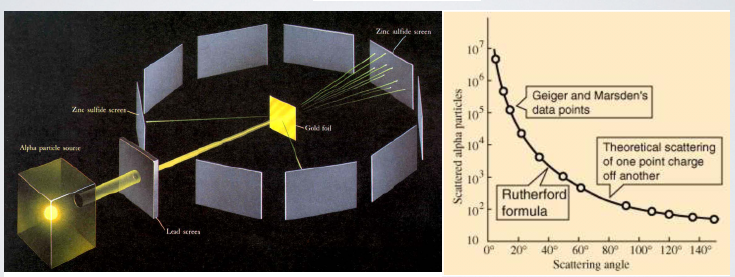
\includegraphics[scale=0.75]{Images1/geiger.PNG}
    \caption{Expérience de Geiger et Marsden : Dispositif - Comparaison prédictions/mesures}
    \label{fig:geiger_marsden}
\end{figure}

Plusieurs minutes après la disposition du matériel, différents points lumineux apparaissent sur l'écran et ces points ne sont pas tous dans l'orientation du faisceau, mais certains étalés sur de grands angles. Rutherford eut ainsi la surprise d'observer une sorte de rebond des particules alpha.

La rétrodiffusion de particules $\alpha$ ne peut s’expliquer que par des chocs élastiques entre les particules alpha et des noyaux atomiques beaucoup plus massifs! Le modèle atomique du flan aux raisins ne résiste évidemment pas à ces observations qui mèneront au modèle de Rutherford (Fig. \ref{fig:mod_rutherford}).
\begin{figure}[ht]
    \centering
    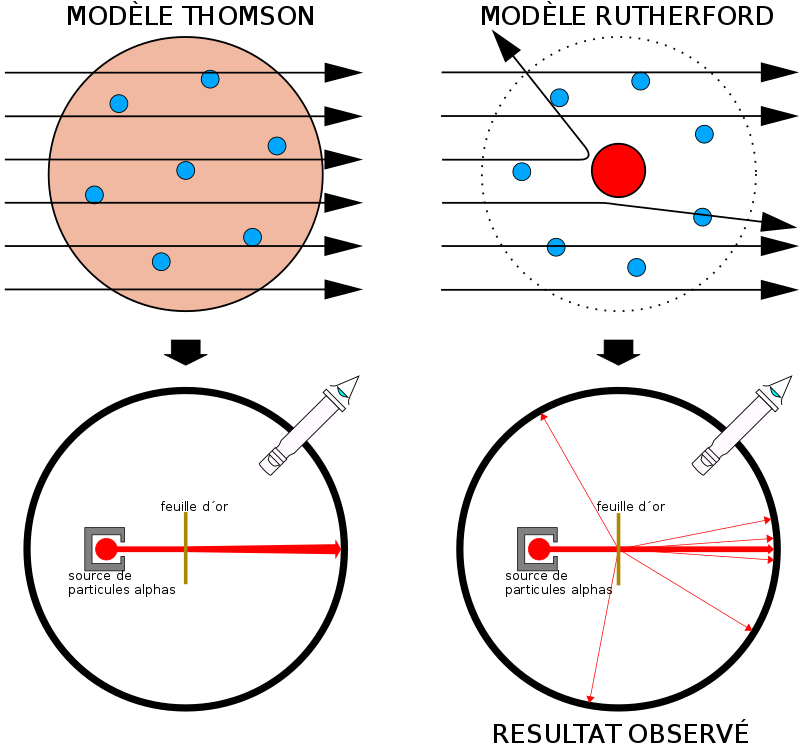
\includegraphics[scale=0.25]{Images1/thom_ruth.png}
    \caption{Modèle de Thomson VS modèle de Rutherford}
    \label{fig:mod_rutherford}
\end{figure}
La distance d'approche minimale calculée par Rutherford satisfait à l'équation

$$\dfrac{1}{2}mv_0^2=\dfrac{1}{4\pi\epsilon_0}\dfrac{Zze^2}{r_\text{min}}$$

Si on projette des $\alpha$ de plus haute énergie sur du plomb par exemple, on observe une diminution du nombre de particules rétrodiffusées à cause de l'interaction forte à courte distance. En effet, les $\alpha$ sont alors absorbés par les noyaux.

\subsection{Découverte du proton}
En 1914, on veut élaborer une théorie du noyau. De quels éléments dispose-t-on ? Le numéro atomique Z, la masse atomique A, le fait qu'un même élément chimique puisse exister sous forme de plusieurs isotopes avec A différents, la radioactivité alpha (il y a des particules alpha, qui sont des noyaux d'hélium, dans certains noyaux), la radioactivité beta (il y a des particules beta, qui sont des électrons, dans certains noyaux). \\
En 1911, Rutherford part des 2 observations que pour la plupart des noyaux, $A \sim 2Z$ et que certains noyaux émettent des particules alpha. Il suggère donc que tous les noyaux, hormis l'hydrogène, sont des assemblages de particules alpha. \\
Cependant, beaucoup d'arguments s'opposent à cette théorie: la moitié des charges électriques Z sont impaires, les masses de la plupart des éléments lourds sont supérieures au double de leur charge électrique, et l'écart s'accroit avec la masse (exemple: du Fer A=56, Z=26 au Plomb A=207, Z=82).  Cela suggère un modèle mixte: hélium + autre chose ? Alors, pourquoi ne pas former directement les noyaux par des assemblages de noyaux d'hydrogène, puisque la plupart des masses atomiques sont des multiples entiers de la masse de l'hydrogène ? Il existe une objection majeure à cette proposition : si on forme le noyau de masse A avec A noyaux d'hydrogène, ce noyau a une charge électrique +Ae, et non +Ze... Rutherford suppose alors à l'époque que le noyau possède en plus A-Z électrons, ce qui expliquerait en plus que les noyaux perdent des électrons dans la radioactivité beta. Cette théorie du noyau avait 2 conséquences:

\begin{itemize}
    \item Il y a des noyaux d'hydrogène dans TOUS les noyaux
    \item Il doit exister un mécanisme séparant les Z électrons dits périphériques des A-Z électrons nucléaires.
\end{itemize}

Le premier point a des conséquences expérimentales un peu étranges que Rutherford mit en avant: en 1915, avec Marsden il bombarde de l'hydrogène avec des particules alpha (source = radon), à l'aide du dispositif illustré ci-dessous. La chambre est remplie de gaz, une source d’alphas (la plaque sur le pied) les projette sur les noyaux du gaz (Fig. \ref{fig:chambre_bombardement_H}). Les alphas, les noyaux du gaz et les protons provoquent des scintillations différentes sur l’écran de sulfure de zinc à droite, observé au microscope. Ils observent des reculs de l'hydrogène, caractérisés par des traces plus fines que celles des alphas.

\begin{figure}[ht]
    \centering
    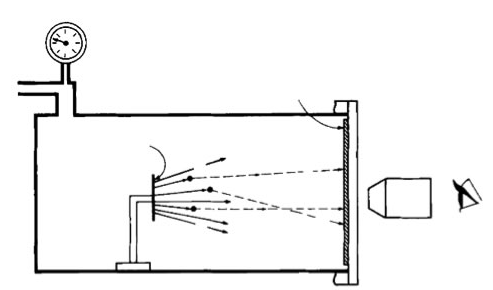
\includegraphics[scale=0.75]{Images1/bombardement.PNG}
    \caption{Chambre de bombardement d'hydrogène}
    \label{fig:chambre_bombardement_H}
\end{figure}

Marsden remarqua une émission d'hydrogène par le radon avant le remplissage de la chambre en hydrogène. Rutherford ne crut pas à une nouvelle forme de radioactivité, mais plutôt à une contamination de l'appareillage par l'hydrogène. Il nota plus tard que s'il remplissait la chambre d'oxygène ou de gaz carbonique, le nombre de scintillations attribuables à l'hydrogène diminuait, comme il s'y attendait, mais ce nombre augmentait quand la chambre était remplie d'air et plus encore quand elle était remplie d'azote ! Ce phénomène de <<fuite d'hydrogène>> n'apparaissait que pour des alphas d'énergie supérieure à 1.21 \si{MeV}. Rutherford supposa donc une ionisation des molécules d'eau présentes dans l'air ou l'azote. Mais après suppression de l'eau, le phénomène persistait, Rutherford en conclut donc que l'azote se transmutait au cours de la collision avec les alphas, et que les noyaux d'hydrogène appartenaient au noyau d'azote. Rutherford pensait observer la réaction
\begin{center}
    alpha + azote $\longrightarrow$ hydrogène + carbone + alpha
\end{center}
et son interprétation fut la suivante en 1919 :

\begin{itemize}
    \item Carbone: masse atomique 12 = 3 alphas
    \item Oxygène: masse atomique 16 = 4 alphas
    \item Azote: masse atomique 14 = 3 alphas + 2 hydrogènes périphériques, facilement arrachables par l’alpha servant de projectile, dès qu’il avait une énergie suffisante (les 1.21 \si{MeV} requis)
\end{itemize}

Cette interprétation a 2 conséquences majeures: les transmutations nucléaires ne sont pas limitées aux éléments lourds (radioactifs) et les collisions d'alphas permettent de sonder en profondeur les noyaux, pas seulement leur cortège d'électrons.

Rutherford a ainsi développé une nouvelle technique de recherche, malheureusement limitée par la faible énergie des alphas. S'en suivit pour remédier à ce problème la conception d'accélérateurs, comme le premier cyclotron, par Lawrence (Fig. \ref{fig:lawrence_cyclo}).

L’utilisation de la chambre de Wilson (ou chambre à brouillard) (Fig. \ref{fig:chambre_wilson}) se révéla bien plus pratique que les écrans au sulfure de zinc, car elle permettait de visualiser, et d’enregistrer, le résultat des collisions sous la forme de traces des particules avant et après collision, et même parfois de mesurer leur charge et leur énergie. En 1920, Chadwick mesura la charge des noyaux Cu, Ag, Pt par diffusion alphas. Ayant démontré qu’il y avait bien des noyaux d’hydrogène dans le noyau d’azote, Rutherford les baptisa proton en 1920.

\begin{figure}[ht]
    \centering
    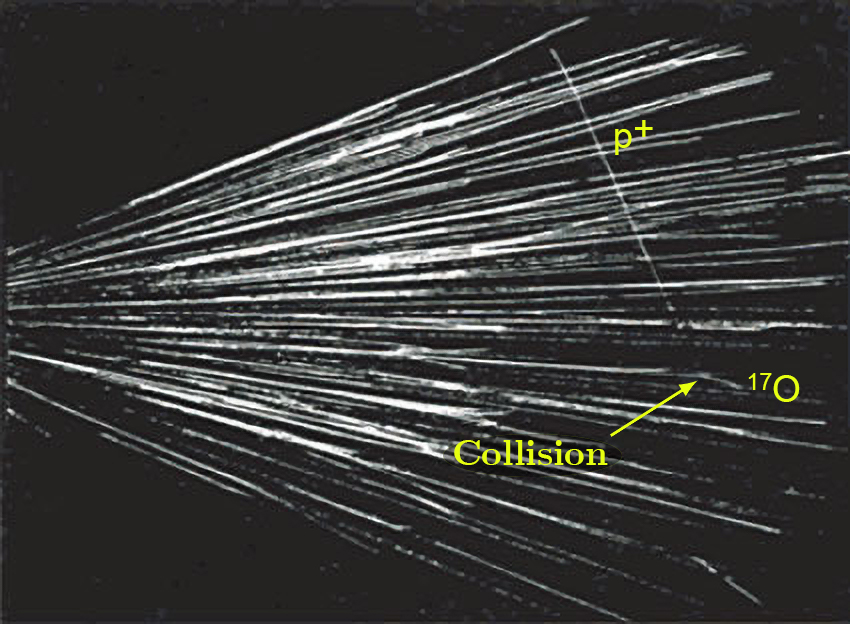
\includegraphics[width=0.7\textwidth]{Images1/collisions_alpha_proton.jpg}
    \caption{La chambre à brouillard de Wilson: des particules alpha provenant d'une source sur la gauche laissent une traînée des gouttelettes dans une chambre à brouillard remplie d'azote. L'une d'entre elles frappe un noyau d'azote à droite, donnant un proton partant vers le haut gauche et un noyau d'oxygène partant vers le bas à droite. (Blackett 1935)}
    \label{fig:chambre_wilson}
\end{figure}

Les expériences de Rutherford validaient --- apparemment --- l’image du noyau comme un assemblage de A protons avec A-Z électrons <<nucléaires>>, associés pensait-il en sous-structures alpha. De nombreux modèles qualitatifs furent élaborés pour rendre compte des régularités empiriques, mais ils étaient peu prédictifs, et surtout ils entrèrent très vite en conflit avec la nouvelle mécanique quantique (Fig. \ref{fig:to_be_continued})...

\begin{figure}[ht]
    \centering
    \begin{minipage}{.5\textwidth}
        \centering
        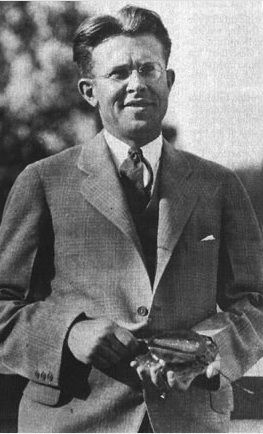
\includegraphics[height=5.5cm]{Images1/cyclo.PNG}
        \captionof{figure}{Lawrence et un bébé cyclotron}
        \label{fig:lawrence_cyclo}
    \end{minipage}%
    \begin{minipage}{.5\textwidth}
        \centering
        
\includegraphics[height=5.5cm]{Images1/mama.png}
        \captionof{figure}{To be continued...}
        \label{fig:to_be_continued}
    \end{minipage}
\end{figure}

\subsection{Découverte du neutron}
En gros:
\begin{itemize}
    \item 1931: Joliot et sa femme Curie bombardent du Béryllium avec une source d'alpha et observent une radiation très pénétrante (Fig. \ref{fig:joliot_curie}).

    \begin{figure}[H]
        \centering
        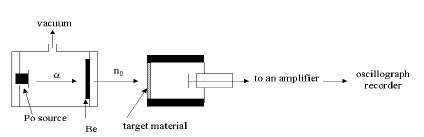
\includegraphics[scale=0.99]{Images1/joliotcurie.PNG}
        \caption{Expérience de Joliot-Curie}
        \label{fig:joliot_curie}
    \end{figure}

    Hypothèse de Bothe et Becker: ce sont des rayons X. Hypothèse de Joliot et Curie: ce sont des rayons gamma, et la réaction est donc similaire à celle de l'effet Compton sur des protons. Ils pensent cela, car ils observent l'émission de protons éjectés d'une cible de paraffine bombardée avec cette radiation. (protons mesurés avec une chambre à ionisation.) Hypothèse de Chadwick: la radiation correspond à une interaction avec une nouvelle particule neutre donc la masse est similaire à celle du proton selon la réaction
    \[
        ^{4}_{2}He + ^{9}_{4}Be \rightarrow ^{12}_{6}C + ^{1}_{0}n
    \]

    \item Il mesure que les protons éjectés ont des vitesses maximales $v=\dfrac{c}{10}$ dans une chambre à brouillard, compatible avec des photons de \SI{50}{MeV} incidents, ce qui est très élevé pour des rayons gamma qui ont normalement une énergie de quelques \si{MeV}.

    \item Il note le recul de noyaux d'azote si l'azote est introduit dans la chambre à brouillard (Fig \ref{fig:recul_azote}) ! Ici aussi, le parcours de l'azote dans le chambre est tel que l'énergie est bien plus élevée que 400 \si{keV} (qui serait l'énergie maximale si on avait des photons de \SI{50}{MeV})


    \begin{figure}[ht]
        \centering
        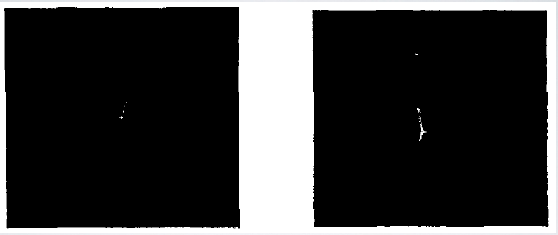
\includegraphics[scale=0.85]{Images1/reculazote.PNG}
        \caption{Gauche: Recul de ce qui pourrait être un ion d'azote - Droite: Recul d'un ion d'azote qui fait interaction élastique avec un autre noyau d'azote}
        \label{fig:recul_azote}
    \end{figure}

    \item Il observe aussi d'autres réactions inélastiques type $n + ^{14}N \rightarrow ^{11}B + \alpha $ (voir figure \ref{fig:coll_inelastique})

    \begin{figure}[ht]
        \centering
        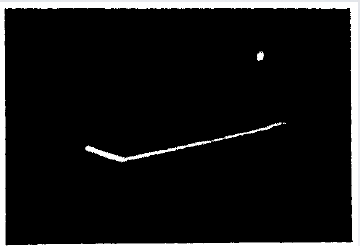
\includegraphics[scale=0.80]{Images1/inelastique.PNG}
        \caption{Réactions inélastiques entre un neutron et l'azote de la chambre}
        \label{fig:coll_inelastique}
    \end{figure}
\end{itemize}
Comment a-t-on déterminé la masse de la nouvelle particule, le neutron ? Pour la collision
\[
    m + M \rightarrow m + M
\]
où m a une vitesse initiale v et M est au repos, on a que la vitesse maximale de M après la collision est
\[
    \dfrac{2mv}{(m+M)}
\]
Sachant que les vitesses maximales pour le proton de recul et l'azote sont respectivement \SI{3.7e9}{cm/s} et \SI{1.7e8}{cm/s}, on obtient $m$ = $90\%~M_\text{proton}$. En bons physiciens, on considère donc que $M_\text{proton}$ = $M_{neutron}$. (En vrai, des mesures plus précises ont indiqué que la différence entre le deux vaut 0,14 pour cent de la masse moyenne du proton et du neutron.)

\subsection{Mesure de la masse des noyaux et énergie de liaison}
Expérimentalement, on détermine la masse des noyaux via la technique de spectrographie de masse (Fig. \ref{fig:spectro_masse}). Elle consiste à identifier les masses des composants d'un échantillon de manière individuelle grâce à un faisceau d'ions. Une source produit ce faisceau possédant une certaine distribution de vitesses. Un sélecteur de vitesses permet seulement aux ions ayant une vitesse particulière de passer (le reste du faisceau est défléchi), et la sélection de moments grâce à un champ magnétique permet l'identification des masses individuelles.
\begin{figure}[ht]
    \centering
    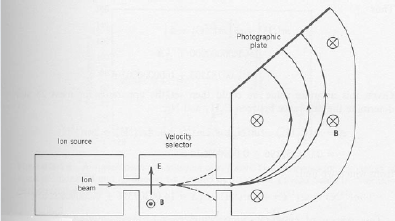
\includegraphics[scale=0.80]{Images1/spectro.PNG}
    \caption{Principe du spectrographe de masse}
    \label{fig:spectro_masse}
\end{figure}
Soit un atome avec A nucléons, Z protons et Z électrons. Sa masse M(A,Z) s'écrit
\[
    M(A,Z) = m(A,Z) + Z \cdot m_e - E^{\text{atome}}_{\text{liaison}}
\]
avec m(A,Z) la masse du noyau de l'atome, définie par
\[
m(A,Z)=Z.m_p+(A-Z)m_n-E^{\text{nucléaire}}_{\text{liaison}}
\]
Définissons l'énergie de liaison de l'atome par
\[
    B=E^\text{atome}_\text{liaison}+E^{\text{noyau}}_{\text{liaison}}
\]
Elle est largement dominée par l'énergie de liaison nucléaire de sorte que dans la suite, on approximera B comme l'énergie de liaison du noyau. Cette énergie de liaison est généralement négligeable devant l'énergie de masse.
En guise d'exemple, on considère le système de 2 nucléons (le deutérium). Évaluons l'énergie de liaison de son noyau, le deuton. On a
\[
    M(^{2}_{}D)=2.014~u
\]
où \[u=\dfrac{1}{12}M(^{12}_{}C)=931.495 \cdot \dfrac{\si{MeV}}{c^2}=\SI{1.66054e-27}{kg}\]
Connaissant les masses du proton, neutron et électron, on trouve que
\[
    B(^{2}_{}D) = \SI{2.227}{MeV}/c^2
\]
soit $0.12\%~M(^{2}_{}D)$.

\subsection{Découverte des rayons cosmiques et de l'antimatière}
Le rayonnement cosmique est le flux de noyaux atomiques et de particules de haute énergie (relativistes) qui circulent dans le milieu interstellaire. La source de ce rayonnement se situe selon les cas dans le Soleil, à l'intérieur ou à l'extérieur de notre galaxie. Certaines astroparticules qui composent le rayonnement cosmique ont une énergie qui dépasse 1020 eV et qui n'est expliquée par aucun processus physique identifié. Le rayonnement cosmique est principalement constitué de particules chargées : protons, noyaux d'hélium, antiprotons, électrons, positrons et particules neutres (rayons gamma, neutrinos et neutrons).\\[0,2cm]
La découverte du rayonnement cosmique a lieu au début du XXe siècle avec les observations de Victor Hess effectuées en 1912 depuis un ballon. Il observe une légère diminution du taux de décharge de l'électroscope entre 0 et 500m d'altitude (mesure effectuée initialement entre la base de la tour Eiffel et son sommet, à 324m d'altitude).

\begin{figure}[ht]
    \centering
    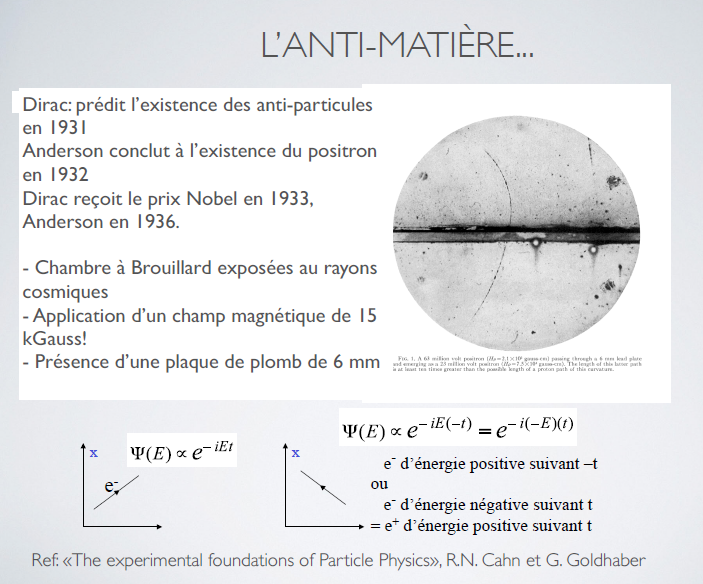
\includegraphics[scale=0.80]{Images1/antimatiere.PNG}
    \caption{Découverte de l'antimatière}
\end{figure}
\newpage

\clearpage

\part{Physique atomique (Xavier Urbain et Mariko Terao)}
\begin{center}
    En cas de questions ou de remarques sur cette partie : contactez Eléonore Lieffrig, Justin Gérard %ou Valentin Fonck.
\end{center}
Concernant cette partie, 2 syllabus écrits par Prof. Mariko Terao sont disponibles sur Moodle. Il reste donc les slides de Xavier Urbain à traiter.

\section{Rappels sur l'atome d'hydrogène}

\subsection{Mise en contexte du problème}

Considérons l'atome d'hydrogène où $M$ et $m$ sont respectivement la masse du noyau et la masse de l'électron. Soit $\Psi$ la fonction d'onde du système. L'évolution de cette dernière est bien entendu décrite par l'équation de Schrödinger:

\[\imag\hbar \dfrac{\partial}{\partial t}\Psi=H\Psi\]

où \begin{align}
H&\eq T+V \\
&\eq -\dfrac{\hbar^2}{2\mu}\nabla^2-\dfrac{Ze^2}{4\pi \epsilon_0 r}
\end{align}
avec $\mu=\dfrac{Mm}{(m+M)}$ la masse réduite du système et $r$ la distance entre le noyau et l'électron. Le potentiel $V$ étant dans ce cas indépendant du temps, on peut montrer que les solutions de l'équation de Schrödinger sont de la forme

\[
    \Psi(\Vec{r},t) \eq \Psi_E(\Vec{r}) \cdot \exp(-\dfrac{\imag}{\hbar}Et)
\]


On va chercher les états stationnaires tels que $H\Psi_E=E\Psi_E$ (équation de Schrödinger indépendante du temps), $\Psi_E(\Vec{r})$ étant la fonction d'onde au temps $t=0$. Pour cela, réécrivons la contribution cinétique à l'hamiltonien en coordonnées sphériques. Cela nous permettra de séparer notre équation en une partie radiale et une partie angulaire où apparaîtra l'opérateur moment angulaire $L^2$. Ce dernier sera qualifié de terme "centrifuge" en référence à l'effet de rotation du système, qui est la propriété de $L^2$.

\subsection{Passage aux coordonnées sphériques}

En coordonnées sphériques,

\begin{align*}
    T&\eq
    \dfrac{-\hbar^2}{2\mu}\left[\dfrac{1}{r^2}\dfrac{\partial}{\partial r}\left(r^2\dfrac{\partial}{\partial r}\right)+\dfrac{1}{r^2\sin{\theta}}\dfrac{\partial}{\partial \theta}\left(\sin{\theta}\dfrac{\partial}{\partial \theta}\right)+\dfrac{1}{r^2(\sin{\theta})^2}\dfrac{\partial ^2}{\partial\phi^2}\right]\\
    &\eq-\dfrac{\hbar^2}{2\mu}\left[\dfrac{1}{r^2}\dfrac{\partial}{\partial r}\left(r^2\dfrac{\partial}{\partial r}\right)-\dfrac{\Vec{L}^2}{\hbar^2r^2}\right]
\end{align*}
Les opérateurs $H$, $L_z$ et$\Vec{L}^2$ commutent entre eux. Cela signifie qu'ils possèdent un ensemble commun de fonctions propres. Or, on sait que les fonctions propres des opérateurs $\Vec{L}^2$ et $L_z$ sont les harmoniques sphériques

\begin{align*}
    Y_{lm}(\theta, \phi) \eq (-1)^m \left[ \dfrac{(2l+1)(l-m)!}{4\pi(l+m)!}\right]^{1/2} \cdot P^{l}_{m}(\cos{\theta})e^{im\phi} \qquad m\ge0
\end{align*}
Rappelons donc quelques identités impliquant les harmoniques sphériques:


\[
    Y_{l}^{-m}(\theta, \phi)\eq (-1)^m\left[Y_{l}^{m}(\theta, \phi)\right]^{*}
\]

\[
    L^2Y_{lm}\eq-\hbar^2 \left[\dfrac{1}{\sin{\theta}}\dfrac{\partial}{\partial\theta}\left(\sin{\theta}\dfrac{\partial}{\partial\theta}\right)+\dfrac{1}{\sin{\theta}^2}\dfrac{\partial^2}{\partial\phi^2}\right]Y_{lm}\eq l(l+1)\hbar^2Y_{lm}
\]

\[
    L_zY_{lm}\eq-\imag\hbar\dfrac{\partial}{\partial\phi}Y_{lm}\eq m\hbar Y_{lm}
\]
Les harmoniques sphériques sont donc bien des fonctions propres de $L^2$ (resp. $L_z$) de valeurs propres $l(l+1)\hbar^2$ (resp. $m\hbar$). Etant donné que les opérateurs $H$, $L_z$ et $L^2$ commutent, les harmoniques sphériques sont également fonctions propres de $H$. Ainsi, ces dernières sont forcément de la forme

\[
    \Psi_{Elm}(r,\theta,\phi)\eq R Y_{lm}(\theta,\phi)
\]
où $R$ est un facteur indépendant des coordonnées angulaires. Les fonctions propres de $H$ étant dépendantes de ces coordonnées angulaires mais également de $r$, le facteur $R$ doit donc être fonction de $r$, ce qui donne finalement

\begin{equation}
    \Psi_{Elm}(r,\theta,\phi)\eq R_{Elm}(r) Y_{lm}(\theta,\phi)
    \label{decompopsi}
\end{equation}



\subsection{Constantes du mouvement}
Considérons l'équation de Schrödinger et sa complexe conjuguée:

\[
    \imag \hbar \dfrac{\partial}{\partial t} \Psi \eq H \Psi
\]

\[
    -\imag \hbar \dfrac{\partial}{\partial t} \Psi ^{*}\eq (H \Psi)^{*}
\]
Le taux de variation au cours du temps de la valeur moyenne d'un opérateur $A$ est donc donnée par

\begin{align*}
    \fdif{}{t}  \braket{A} &\eq\fdif{}{t} \int \Psi^{*} A \Psi \dif\vec{r} \\
    &\eq \int\left(\dfrac{\partial\Psi^{*}}{\partial t}A \Psi + \Psi^{*} A \dfrac{\partial \Psi }{\partial t } + \Psi^{*} \dfrac{\partial A}{\partial t}\Psi \right) \dif\vec{r}\\
    &\eq \Big< \dfrac{\partial A}{\partial t} \Big> +\dfrac{1}{\imag \hbar} \int \Psi^{*} (AH-HA)\Psi \dif\vec{r}
\end{align*}
Dans le cas particulier où l'opérateur $A$ est indépendant du temps, on a


\[
  \fdif{}{t}\left<A\right>\eq \dfrac{1}{\imag\hbar}\big<[A,H]\big>
\]
Ainsi, si $A$ commute avec l'hamiltonien $H$, sa valeur moyenne ne varie pas au cours du temps, c'est une constante du mouvement ($\equiv$ grandeur ne variant pas lors de l'évolution du système).


\subsection{Séparation des variables: équation radiale}
Revenons\footnote{pour ceux qui veulent, un développement assez similaire est fait de
manière plus claire dans le chapitre 4 de Quantique 2} à l'équation \eqref{decompopsi}

\[
    \Psi_{Elm}(r, \theta, \phi)\eq R_{El}(r)Y_{lm}(\theta, \phi)
\]
Si on substitue cette décomposition dans l'équation de Schrödinger indépendante du temps $H\Psi_E=E\Psi_E$ avec l'expression de $T$ que l'on avait développée en coordonnées sphériques, on trouve que la fonction radiale $R_{El}$ doit satisfaire à

\begin{equation}
    \left[-\dfrac{\hbar^2}{2\mu}\left[\dfrac{1}{r^2}\fdif{}{r}\left(r^2\fdif{}{r}\right) - \dfrac{l(l+1)}{r^2}\right]+V(r)\right]R_{El}(r)\eq ER_{El}(r)
    \label{44}
\end{equation}
Posons $R_{El}(r)\eq \dfrac{1}{r}u_{El}(r)$. \eqref{44} devient

\[
    \left[-\dfrac{\hbar^2}{2\mu}\ffdif{}{r}+\dfrac{l(l+1)\hbar^2}{2 \mu r^2}+V(r)\right] u_{El}(r)\eq Eu_{El}(r)
\]
$\dfrac{l(l+1)\hbar^2}{2\mu r^2}$ est un terme de répulsion (répulsion centrifuge plus exactement). En r=0, il faut que la fonction d'onde réduite s'annule pour éviter la divergence:

\[u_{El}(0)=0\]
On a

\begin{equation}
    \left[\ffdif{}{r}+\dfrac{2\mu}{\hbar^2}[E-V_\text{eff}(r)]\right]u_{El}(r)\eq 0
    \label{jsp}
\end{equation}
où on a défini le potentiel effectif

\[
    V_\text{eff}(r)\eq -\dfrac{Ze^2}{4\pi \epsilon_0}\dfrac{1}{r}+\dfrac{l(l+1)\hbar^2}{2\mu r^2}
\]
Le premier terme est le potentiel coulombien et le deuxième est le `potentiel' centrifuge. Plus $l$ est grand, plus ce potentiel s'ajoutant au coulombien va être grand près de l'origine, ce qui va pousser la fonction d'onde à plus grande distance. On a un effet similaire sur un carrousel : un point sur un carrousel tournant ressentira une force voulant l'expulser de l'attraction.

la figure \ref{fig:potentieleffectif} représente le potentiel effectif pour différentes valeurs de $l$ (et pour Z=1).

\begin{figure}[htp]
    \centering
    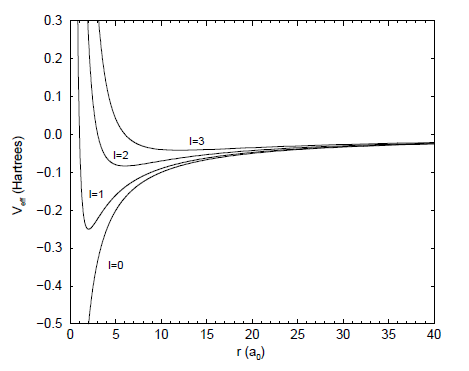
\includegraphics[scale=0.80]{Images2/rad.PNG}
    \caption{Potentiel effectif $V_\text{eff}$ pour Z=1}
    \label{fig:potentieleffectif}
\end{figure}
A courte distance, on observe que le terme en $\dfrac{1}{r^2}$ domine. Sans moment angulaire, on a juste un potentiel coulombien. En ajoutant un terme en $\dfrac{1}{r^2}$ ("potentiel centrifuge", n'existe que quand on a un moment angulaire non nul) on obtient une barrière de potentiel à courte distance. Ainsi, le moment angulaire va empêcher l'électron d'approcher du noyau (c'est-à-dire du proton dans notre cas de l'hydrogène). On s'attend donc, lorsque qu'on va calculer la fonction d'onde radiale, à ce qu'elle soit localisée près du noyau lorsque $l=0$ et de plus en plus loin du noyau au fur et à mesure que $l$ grandit.


Il est possible de faire en sorte que l'équation soit plus simple et en unités réduites. Pour que le comportement colle avec ce qu'on sait déjà, il faut qu'à l'infini la probabilité de présence de l'électron tende exponentiellement vers 0, quelque soit la valeur de $l$ car quand on s'éloigne, on atteint une zone où l'énergie totale est inférieure à l'énergie potentielle donc la probabilité de présence de l'onde dans cette zone doit tendre vers 0. C'est une région qui est classiquement interdite, mais tenant compte des effets tunnels, la fonction d'onde y est présente, mais décroît de façon exponentielle.


Posons, pour simplifier les notations, les quantités sans dimension

\[
    \rho\eq\left(-\dfrac{8\mu E}{\hbar^2}\right)^{1/2}r
\]

\begin{equation}
    \lambda\eq\dfrac{Ze^2}{4\pi\epsilon_0 \hbar}\left(-\dfrac{\mu}{2E}\right)^{1/2}\eq Z\alpha\left(-\dfrac{\mu c^2}{2E}\right)^{1/2}
    \label{lambda}
\end{equation}
où $\alpha=e^2/(4\pi\epsilon_0 \hbar c) \approx 1/137$ est la constante de structure fine. Cela nous permet de réécrire l'équation \eqref{jsp} comme


\begin{equation}
    \left[\ffdif{}{\rho}-\dfrac{l(l+1)}{\rho^2}+\dfrac{\lambda}{\rho}-\dfrac{1}{4}\right]u_{El}(\rho)\eq0
    \label{reduite}
\end{equation}
Lorsque $\rho \rightarrow +\infty$, les termes en $\dfrac{1}{\rho}$ et $\dfrac{1}{\rho^2}$ sont négligeables et alors les 2 solutions de \eqref{reduite} sont de la forme exp$(\pm \rho/2)$. Comme on cherche des solutions bornées, on ne garde que la solution asymptotiquement décroissante et donc on a la condition suivante sur notre solution:

\[
    u_{El}(\rho)\sim e^{-\rho/2} \quad \text{pour} \quad \rho \longrightarrow \infty
\]
Ainsi, la fonction $u_{El}(\rho)$ doit être de la forme

\[
    u_{El}(\rho)\eq e^{-\rho/2}f_{El}(\rho)
\]
avec $f_{El}(\rho)$ satisfaisant l'équation

\begin{equation}
 \left[\fdif{}{\rho^2}-\fdif{}{\rho}-\dfrac{l(l+1)}{\rho^2}+\dfrac{\lambda}{\rho}\right]f_{El}(\rho)\eq0
 \label{fel}
\end{equation}
De plus, quand $\rho \longrightarrow 0$, c'est le terme en $1/\rho^2$ qui devient dominant dans \eqref{reduite}. La solution régulière est de la forme

\[
    u_{El}(\rho) \sim \rho^{l+1} \qquad \text{pour} \qquad \rho \longrightarrow 0
\]
Supposons que $f_{El}(\rho)$ puisse s'écrire sous la forme

\[
    f_{El}(\rho)\eq\rho^{l+1}g_{El}(\rho)
\]
où on développe $g_{El}$ en série:

\[
    g_{El}(\rho)\eq\sum_{k=0}^{\infty} c_k\rho^k \quad c_0 \neq 0
\]
En injectant ce développement de solution dans \eqref{fel}, on obtient l'équation que doit satisfaire $g_{El}(\rho)$:

\begin{equation}
    \left[\rho\ffdif{}{\rho}+(2l+2-\rho)\fdif{}{\rho}+(\lambda-l-1)\right]g_{El}(\rho)\eq0
    \label{gel}
\end{equation}
En y substituant notre développement en série, on obtient la relation de récurrence que doivent satisfaire les coefficients $c_k$:

\begin{equation}
    c_{k+1}\eq\dfrac{k+l+1-\lambda}{(k+1)(k+2l+2)}c_k
\end{equation}
Supposons que $g_{El}(\rho)$ soit un polynôme de degré $n_r$. Comme il doit être fini, il faut que $c_{n_{r}+1}$=0 du coup

\[
    n_r+l+1-\lambda\eq0 \quad \Rightarrow \quad \lambda\eq n_r +l+1
\]
$\lambda$ est donc un nombre entier positif. On l'appelle nombre quantique principal de la solution et on le note $n$. La relation \eqref{lambda} fournit la valeur propre $E_n$ de la solution:

\begin{equation}
    E_n\eq -\dfrac{1}{2n^2}\left(\dfrac{Ze^2}{4\pi\epsilon_0}\right)^2\dfrac{\mu}{\hbar^2}\eq -\dfrac{1}{2}\mu c^2 \dfrac{(Z\alpha)^2}{n^2}
\end{equation}

Le spectre d'énergie de l'atome d'hydrogène (c'est-à-dire les valeurs de l'énergie pour différents $n$) est représenté à la figure \ref{fig:spectreH}.
\begin{figure}[htp]
    \centering
    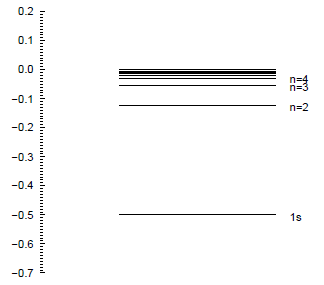
\includegraphics{Images2/spectreH.PNG}
    \caption{Spectre d'énergies de l'atome d'hydrogène. Les énergies sont exprimées en Hartree}
    \label{fig:spectreH}
\end{figure}
Pour chaque nombre quantique principal, on a un certain nombre de sous-niveaux qui est croissant avec $n$ (pour $n=1$ on a le niveau 1s, pour $n=2$ on a 2s et 2p,...). Il y a donc une dégénérescence des niveaux d'énergie qui peuvent donc correspondre à des fonctions d'onde différentes, ce qui va compliquer le spectre. Cette dégénérescence est due (c'est non trivial) à la dépendance en $r^{-1}$ du potentiel coulombien et peut être levée par l'action d'un champ électrique ou magnétique (effets Stark et Zeeman).

Comme la puissance du polynôme $g_{El}$ vaut $n_r=n-l-1$ qui est forcément nul ou positif, il y a $n-1$ valeurs possibles de $l$ pour chaque valeur de $n$: $l=0, 1, ..., n-1$. De plus il y a $2l+1$ valeurs possibles de $m$ pour chaque valeur de $l$: $m=-l, -l+1, ..., l-1, l$. Le degré de dégénérescence du niveau $E_n$ vaut donc

\[
    \sum_{l=0}^{n-1} (2l+1)\eq 2\sum_{l=0}^{n-1} l + n \eq  2 \dfrac{(n-1)n}{2} + n \eq  n^2
\]
On remarque un tassement des niveaux vers la limite d'ionisation (région entre $n=2$ et $n=\infty$).

\subsection{Solution complète}
Il se trouve que les polynômes $g_{El}(\rho)$ sont des polynômes de Laguerre associés. En effet ceux-ci sont définis comme solutions de l'équation différentielle

\begin{equation}
    \left[x\ffdif{}{x}+(K+1-x)\fdif{}{x}+N\right] L_{N}^{K}(x)\eq 0
\end{equation}
L'équation \eqref{gel} est similaire à cette équation, et en les comparant on en déduit même que

\[
    g_{El}(\rho)\eq L_{n-l-1}^{2l+1}(\rho)
\]
En regroupant les résultats des sous-sections précédentes on a donc comme solution pour les fonctions d'onde normalisées des états liés de l'atome d'hydrogène:

\begin{equation}
    \Psi_{nlm}(r,\theta,\phi)\eq -\left[\left(\dfrac{2Z}{na_{\mu}}\right)^3\dfrac{(n-l-1)!}{2n[(n+l)!]^3}\right]^{1/2}e^{-\rho/2}\rho^l L_{n-l-1}^{2l+1}(\rho)Y_{lm}(\theta,\phi)
    \label{sol}
\end{equation}
où on a remplacé l'indice $E$ par $n$ vu que ces 2 quantités sont reliées par une relation univoque.


\subsection{Étude des fonctions d'ondes radiales}
On souhaite développer quelques fonctions radiales pour les états les plus bas du spectre. On considère donc la partie radiale de \eqref{sol} dans laquelle on effectue l'approximation du noyau infiniment lourd ($\mu=m$). Ainsi $a_\mu$ se réduit à

\[
    a_{\mu}\eq \dfrac{4\pi\epsilon_0\hbar^2}{\mu e^2}\eq \dfrac{4\pi\epsilon_0\hbar^2}{me^2}\eq  a_0
\]
qui est le rayon de Bohr. De plus,

\[
    \rho\eq \dfrac{2Z}{n a_{\mu}}r
\]
En s'aidant d'une table contenant les polynômes de Laguerre \textbf{généralisés} (attention il y a les simples et les généralisés !), on obtient les fonctions radiales de la figure \ref{fig:foncrad} pour (dans l'ordre) les états 1s, 2s, 3s, 2p, 3p, 3d.

\begin{figure}[htp]
    \centering
    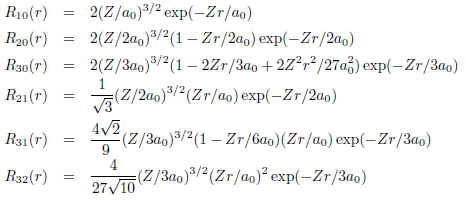
\includegraphics{Images2/foncrad.PNG}
    \caption{Fonctions radiales}
    \label{fig:foncrad}
\end{figure}
On remarque que les fonctions d'onde s ont une amplitude non nulle en $r = 0$, contrairement aux fonctions
d'onde des états $l\neq 0$ qui se comportent en $r^l$ près de l'origine. C'est le potentiel centrifuge $l(l+1)\hbar^2/2\mu r^2$ qui empêche l'électron de pénétrer dans le noyau. Pour une même valeur de n, les états de plus bas $l$ ont une amplitude plus importante près de $r = 0$.

À le figure \ref{fig:fcx_rad_1} sont représentées les fonctions d'onde radiales ($R_{nl}$) et fonctions de distribution radiales ($D_{nl}(r)=r^2|R_{nl}(r)|^2$) (qui est la probabilité par unité de longueur de trouver l'électron à une distance $r$ du noyau) de quelques états de l'atome d'hydrogène ($Z=1$):
\begin{figure}[htp]
    \centering
    \includegraphics[scale=0.8]{Images2/ex.PNG}
    \caption{Fonctions d'onde radiale et de distribution radiale des 4 premiers états s. Le nombre de noeuds est $n-1$}
    \label{fig:fcx_rad_1}
\end{figure}
Quelques remarques à propos de ces figures:

\begin{itemize}[label=$\bullet$]
    \item Si on veut savoir quelle est la probabilité que l'électron se trouve à une distance $r$ du noyau, il faut prendre le carré de la fonction d'onde et intégrer sur le volume, cette probabilité de trouver l'électron dans une coque sphérique comprise entre $r$ et $r+\dif r$ est donc $r^2|R_{nl}(r)|^2\dif r\int \dif\Omega |Y_{lm}(\theta,\phi))|^2$. Il y aura donc apparition d'un facteur $r^2$ venant des coordonnées sphériques. Ce qu'on va calculer c'est donc la densité radiale de probabilité. L'intégrale porte aussi bien sûr sur la partie angulaire de la fonction d'onde mais ce n'est pas ce qui nous intéresse. La densité radiale est en fait la probabilité de présence à une certaine distance $r$ du noyau.
    \item Dans un état 1s, l'électron se trouve à une distance moyenne d'un rayon de Bohr, par définition. Sa distribution est centrée à une unité atomique.
    \item Dans l'état 2s, la majeure partie de la probabilité se trouve à plus grande distance que pour l'état 1s. De 1 u.a. (pour 1s), on est passé à environ 4 u.a. (pour 2s).
    \item Le nuage électronique s'étend rapidement au fur et à mesure que $n$ augmente (évolution en $n^2$)
    \item La courbe de distribution radiale de l'état 1s montre un confinement tout près de $r=0$.
    \item On remarque la présence de lobes sur les courbes, le nombre changeant avec le moment angulaire: en effet les fonction radiales dépendent de $l$.
    \item Les polynômes de Laguerre ont un indice $n-l-1$ et cet indice indique le nombre de noeuds de la fonction.
\end{itemize}

Les figures \ref{fig:fcx_rad_2} et \ref{fig:fcx_rad_3} sont quelques représentations des fonctions d'onde et distributions radiales pour d'autres états.

\begin{figure}[htp]
    \centering
    \includegraphics{Images2/p.PNG}
    \caption{Fonction d'onde radiale et fonction de distribution radiale des 4 premiers états p (courbe 2p bien centrée à 4 rayons de Bohr). La courbe noir correspond à 2p et la courbe bleue à 5p}
    \label{fig:fcx_rad_2}
\end{figure}

\begin{figure}[htp]
    \centering
    \includegraphics{Images2/spdf.PNG}
    \caption{Fonction d'onde radiale et fonction de distribution radiale des états 4s, 4p, 4d et 4f. Le nombre de noeuds est $4-l-1$}
    \label{fig:fcx_rad_3}
\end{figure}

Les états de moment angulaire maximum ($l=n-1$) sont beaucoup plus simples à comprendre que les autres qui ont un comportement ondulatoire (présence de noeuds et ventres dans leur fonction d'onde). En effet, l'électron peut être vu comme une onde piégée dans un potentiel qui va, sous l'action de ce dernier, former une espèce d'onde stationnaire : ce sont les noeuds et les ventres que l'on observe (L'électron a une probabilité de présence nulle sur un noeud et une probabilité forte sur un ventre). On peut donner une image assez classique de ces noeuds et ventres. Lorsqu'on a des noeuds et des ventre, on peut voir l'électron comme une onde stationnaire qui fait des aller-retours entre le noyau et le bord du potentiel. Cependant, lorsque $l$ est maximal (i.e. $l=n-1$), la partie radiale de la fonction d'onde $R_{n,l=n-1}$ ne présente plus qu'un seul ventre sans noeuds. Dès lors, on doit ainsi plus voir l'électron comme orbitant à une distance moyenne constante du noyau. Attention que ceci est une image fort classique pour la mécanique quantique. Cependant plus $n$ est grand, plus on se rapproche de cette image et on peut donc considérer l'électron comme étant une particule classique orbitant autour d'un noyau (surtout à partir de $n=100$).

Plus le nombre quantique $n$ d'un état est élevé, plus l'état correspondant est excité. Un état de grand $n$ est appelé état de Rydberg. A l'échelle atomique, la fonction d'onde d'un tel état s'étend sur de très grandes distances, comme suggère l'expression du maximum de la fonction de distribution radiale

\[
    r\eq \dfrac{n^2}{Z}a_{\mu}
\]
Par exemple, la fonction d'onde radiale de l'état 50s qui est représentée figure \ref{fig:50s} s'étend jusque $5000a_0= \SI{0.27}{\mu m}$.

\begin{figure}[htp]
    \centering
    \includegraphics{Images2/50s.PNG}
    \caption{Fonction d'onde radiale réduite de l'état 50s}
    \label{fig:50s}
\end{figure}





\newpage

\section{Systèmes à électrons non appariés}
\subsection{Introduction : les alcalins}

Les alcalins sont les éléments de la première colonne du tableau périodique. Ils ont une structure électronique à coeur de gaz rare. Ils perdent facilement leur électron de valence célibataire dans la sous-couche externe s. Nous avons par exemple:

\begin{center}
    Li [He:1s$^{2}$] 2s \\
    Na [Ne: 1s$^{2}$2s$^{2}$2p$^{6}$] 3s \\
    K [Ar: 1s$^{2}$2s$^{2}$2p$^{6}$3s$^{2}$3p$^{6}$] 4s
\end{center}
Pour chaque sous-couche pleine, on rappelle qu'on a $\sum_i l_i = 0$.

Nous allons essayer de décrire ces atomes comme un atome d'hydrogène. Tout d'abord, nous nous intéressons au lithium. Dans cette approche de l'atome d'hydrogène on peut voir l'électron 2s comme lié à un ion Li$^{+}$ que l'on peut considérer approximativement comme un proton dans le sens où c'est une charge positive. Puisque c'est un électron 2s, nous savons qu'il a une probabilité de présence non-nulle près du noyau, c'est-à-dire dans le volume occupé par les deux autres électrons.


Étant donné que tout cela est probabiliste, il se peut que l'électron 2s se trouve plus proche du noyau que les autres électrons ("plus proche" d'une façon tout à fait schématique) et que donc il "voit" une charge qui n'est pas $1e$ mais $2e$ ou $3e$ car il n'y a plus d'effet d'écrantage.

Nous avons donc $Z$ qui augmente et l'énergie de liaison $E_n \propto 1/n^2$ aussi. Nous corrigeons par conséquent le nombre quantique principal qui n'est donc plus un nombre entier. Cette correction s’appelle le \textbf{défaut quantique}, notée $\delta_l$, et c’est une bonne solution pour décrire la perturbation de ces électrons dits externes lorsque nous faisons varier le nombre quantique principal.
Le défaut quantique sera toujours du même ordre de grandeur pour tous les alcalins car il ne dépend pas de $n$ mais seulement de $l$. En effet, la probabilité de présence près du noyau de l'électron diminue avec l'augmentation de $l$, donc le défaut quantique sera plus grand pour les plus petits $l$. Pour des moments angulaires plus importants ($l$ élevé), le potentiel effectif (dû au terme centrifuge) va empêcher les électrons externes d’aller à courtes distances et donc ils ne seront pas perturbés par la présence des autres électrons.

\[
    \delta_s>\delta_p>\delta_d>\delta_f\simeq 0
\]
L'énergie de liaison des alcalins obéit à la loi de Balmer modifiée par l’introduction du défaut quantique, qui rend compte de l’écrantage imparfait de la charge du noyau par les autres électrons. Il est d’autant plus grand que l’orbitale a une grande probabilité de présence à courte distance.

\begin{equation}
    E_{nl} \eq  - \dfrac{Ry}{2(n-\delta_l)^2}
    \label{eq:def_quant}
\end{equation}

NB: pas de facteur 2 au dénominateur quand on est en eV ; on est en Hartree dans cette formule.


Si nous nous intéressons maintenant au cas du sodium nous constatons que la correction dépasse 1 pour $l=0$ : $\delta_l = 1.35$. Cela signifie que le remplissage des couches ne se fera pas suivant la règle de Madelung (ou  Klechkowski). \textcolor{red}{Sûr de ça? Parce qu'il y a aussi l'effet joué par la correction du terme $l=1$ à prendre en compte si on veut `classer' les couches}
En effet, pour le potassium (K) par exemple, le 3 de la sous-couche 3d devient 2.75 tandis que le 4 de la sous couche 4s devient 1.81. Par conséquent, l’énergie de la 4s est plus petite que celle du 3d comme l'indique la formule \ref{eq:def_quant}. La sous-couche 4s sera donc remplie avant la 3d.

Ce phénomène ne se limite pas seulement aux alcalins. Pour  n'importe quel atome excité nous pouvons calculer le défaut quantique. (cf exercice sur l'hélium vu en TP).




\subsection{Rayon X}
\subsubsection{Contexte et rappels}


Nous allons ici développer un outil très important pour l'identification des éléments. Il a notamment servi à identifier la présence d'éléments terrestres dans le Soleil, ce qui n'avait a priori rien d'évident. En bombardant un matériau d'électrons de haute énergie, on observe l'émission de rayons X caractéristiques de sa structure.\\

Dans un atome à plusieurs électrons, nous savons que l'énergie ne suit plus exactement la loi de Balmer obtenue pour l'atome d'H ($E_n \propto Z/n^2$). En effet, il y a un effet dû aux autres électrons. Comme nous l'avons vu, cet effet peut être pris en compte en considérant un `défaut quantique' (formule \ref{eq:def_quant}). Cependant, une autre façon de voir les choses est d'utiliser une charge effective mais de laisse le nombre quantique inchangé. Cette charge effective $Z^{*}$ perçue par chaque électron est définie comme \[ Z^{*}=Z-\sigma \] où $\sigma$ représente l'effet d'écran produit sur l'électron d'intérêt par les électrons plus proches du noyau. Dès lors, l'énergie s'exprime comme

\begin{equation}
    E_n \eq -\dfrac{1}{2} \dfrac{(Z-\sigma_n)^2}{n^2} \; [\si{ua} = \si{Ha}]
    \label{eq:energie_effective}
\end{equation}
Comme vu dans l'introduction, lors du passage d'un électron de haute énergie dans un milieu matériel, l'électron subit une perte d'énergie continue sous forme de rayonnement de freinage (pour de hautes énergies de l'électron incident, on peut ignorer la perte sous forme d'ionisation, voir figure \ref{fig:Résumé pertes}). La figure idéalisée de ce rayonnement selon la longueur d'onde de l'électron incident\footnote{On observe donc bien entendu pour un même électron une variation de cette longueur d'onde au cours de sa progression.} se trouve à la figure \ref{fig:Freinage idéalisé} où l'\textit{intensité relative} correspond à l'intensité du rayonnement, autrement dit $\fdif{E}{x}$ la perte d'énergie par unité de distance pour l'électron [\si{J/m}].

\begin{figure}[htp]
    \centering
    \includegraphics[scale=0.8]{Images2/RésuméPerte.PNG}
    \caption{Perte d'énergie par unité de longueur en fonction de l'énergie incidente. On a ici représenté les 2 effets de perte d'énergie dans un matériau : le rayonnement de freinage et la perte par ionisation}
    \label{fig:Résumé pertes}
\end{figure}%
\begin{figure}[htp]
    \centering
    \includegraphics[scale=1.0]{Images2/FreinageIdéalisé.PNG}
    \caption{Rayonnement de freinage sans phénomène de résonance avec les atomes de la cible}
    \label{fig:Freinage idéalisé}
\end{figure}%

Dans la réalité, la perte d'énergie par unité de longueur en fonction de la longueur d'onde incidente est du type de la courbe représentée à la figure \ref{fig:Rayonnement freinage} (et non de la courbe représentée à la figure \ref{fig:Freinage idéalisé} qui n'est qu'une approximation négligeant complètement un phénomène important). Ainsi, pour des longueurs d'onde particulières, la perte d'énergie est drastiquement augmentée. Le phénomène responsable de cette perte drastique est dû à la résonance entre l'énergie de l'électron incident et (dans notre cas présent) des électrons de coeur : l'énergie perdue par les électrons lors de cette résonance correspond à l'énergie des photons associés aux rayons X observés dont nous discuterons dans un instant.\\
\begin{figure}[htp]
    \centering
    \includegraphics[scale=1.0]{Images2/RayonnementFreinage.PNG}
    \caption{Rayonnement de freinage avec résonance avec les niveaux profonds des atomes cibles}
    \label{fig:Rayonnement freinage}
\end{figure}


\subsubsection{Émission de rayons X}


Les fréquences auxquelles on observe les phénomènes de résonance dans le spectre du rayonnement de freinage (= les fréquence où on a des pics d'absorption) correspondent aux fréquences des transitions d'orbitales $n = 2$ vers $n = 1$. Pour caractériser ces transitions, on peut se servir de la loi empirique de Moseley, qui n'est qu'une généralisation des différentes séries de Lyman, Balmer, etc\footnote{En fait, on peut l'obtenir en faisant simplement la différence entre deux niveaux d'énergie distincts via la formule \ref{eq:energie_effective} où on considère un écrantage `moyen' (=la moyenne des écrantages des deux niveaux dont on fait la différence)}.
\begin{equation}
    h\nu
    \eq E_{n_1} - E'_{n_2}
    \eq \dfrac{1}{2}(Z-\sigma_{n_1})^2\left(\dfrac{1}{n_1^2}-\dfrac{1}{n_2^2}\right)
    \label{eq:Moseley}
\end{equation}

Mais dis-moi Jamy, pourquoi est-ce que les atomes émettent ces rayons X? Hé bien Fred, c'est très simple : lors du passage de la particule incidente dans l'atome, on va observer des chocs entre elle et les électrons de coeur (de $n=1$ voire $n=2$) qui sont fortement liés au noyau (en effet, les électrons proche du noyau ne subissent aucun effet d'écrantage atténuant l'action du noyau). Ces chocs avec les électrons de coeur entraînent des trous dans la couche qui sera comblé par la transition d'un électron d'un couche de $n$ plus élevé ($n=2$ sur la figure \ref{fig:Rayons X}). Le rayon X est donc l'émission qui s'associe au passage de l'électron d'une orbitale d'un $n$ élevé à l'orbitale de coeur qui a perdu un électron.
\begin{figure}[htp]
    \centering
    \includegraphics[scale=0.8]{Images2/Rayons X.PNG}
    \caption{Schéma de l'émission de rayons X suite à une ionisation de coeur.}
    \label{fig:Rayons X}
\end{figure}
Grâce aux rayons X, on peut calculer l'effet d'écran d'un certaine couche, c'est-à-dire "de combien la charge du noyau diminue quand on se trouve au-delà de cette couche et donc que les électrons de cette couche agissent comme un écran?". Lors d'une ionisation depuis $n=1$, on a deux électrons dans la couche s1 et donc l'écrantage est approximativement 2. Après ionisation, il ne reste plus qu'un seul électron dans cette couche et par conséquent l'effet d'écran n'est plus que 1 approximativement : Z est à peu près diminué de 1. Ainsi, l'ionisation a bien diminué l'effet d'écran de 1.\\
Pour ce qui est des ionisations de la couche (complète : 8 électrons) $n=2$, on observe après ionisation un effet d'écran de 7.4 dans cette couche de 7 électrons, ce qui est cohérent. Ces valeurs de correction ont été découvertes empiriquement (cfr. l'équation de Moseley \ref{eq:Moseley}).
On calcule donc les fréquences des photons associées aux transitions $2\rightarrow1$ et $3\rightarrow2$:
\[
    \nu_{12}
    \eq \nu_{K_\alpha}
    \eq k (Z - 1)^2 \;[Hz]
\]
\[
    \nu_{23}
    \eq \nu_{L_\alpha}
    \eq k' (Z - 7.4)^2 \;[Hz]
    \;\approx\;  k' (Z - 7)^2 \;[Hz]
\]
où $k$ et $k'$ sont des constantes numériques issues de la formule \ref{eq:Moseley}.



\subsubsection{Émission d'électrons \emph{Auger}}



On sait par la formule \ref{eq:Moseley} que la différence d'énergie entre le seuil d'ionisation et le niveau $n = 2$ est toujours inférieure à la différence d'énergie entre les niveaux 1 et 2. Intéressons-nous à l'émission des "électrons Auger", comme représenté à la figure \ref{fig : Auger}. En fait, lorsqu'un rayonnement ionisant ionise l'électron $1s$, les électrons des couches externes vont venir boucher ce trou en émettant des rayons X. Or, comme rappelé au début de ce paragraphe, l'énergie entre 1s n'importe quel autre niveau est supérieure à l'énergie d'ionisation d'un électron d'un niveau de $n>2$.

Dès lors, dans notre exemple à la figure \ref{fig : Auger}, le rayon X libéré par l'électron $^2P_{1/2}$ a une énergie suffisante pour ioniser l'autre électron $^2P_{1/2}$. Cet autre électron, ionisé, est appelé "électron Auger" et peut en pratique se situer n'importe où ailleurs dans l'atome (il ne se trouve pas forcément au même terme que l'électron qui bouche la couche 1s). Ainsi, on se retrouve avec un atome ayant perdu 2 électrons au total. En outre, on peut avoir 3 électrons manquant à la fin si le rayonnement provoqué par l'ionisation de l'électron Auger ionise encore un autre électron (ce phénomène est moins intense cependant).

Il est dès lors probable que, à la place d'émettre un rayon X, notre atome émette un électron. Cette électron émis aura l'énergie du rayon X (qui est la différence entre les niveaux d'énergie) diminuée du potentiel d'ionisation. On peut ainsi observer un spectre de fréquence à la figure \ref{fig:SpectreAuger} pour ces électrons émis, et ce spectre est structuré de la même façon que le spectre d'émission des rayons X. En fait, la seule différence entre le spectre d'émission d'électrons et le spectre d'émission de rayons X par un atome soumis à un rayonnement ionisant est le potentiel d'ionisation : les électrons doivent effectuer un travail pour sortir de la matière, contrairement aux photons.
\begin{figure}[htp]
    \centering
    \includegraphics[scale=0.8]{Images2/Auger.PNG}
    \caption{Schéma de l'émission d'électrons Auger suite à une ionisation de coeur.}
    \label{fig : Auger}
\end{figure}
\begin{figure}[htp]
    \centering
    \includegraphics[scale=1.0]{Images2/Spectre Auger.PNG}
    \caption{Spectre en fréquence des électrons Auger}
    \label{fig:SpectreAuger}
\end{figure}








\subsection{Le laser}

\subsubsection{Émission spontanée, émission et absorption stimulés}




On détaille ici les équations qui gouvernent ces phénomènes. L'analogie avec la cinétique chimique pour des réactions d'ordre 1 ou la radioactivité est directe. "Un atome ne vieillit pas" et un état non plus, la probabilité de transition par unité de temps est donc une constante.\\
Nous allons donc dans cette section décrire les différents phénomènes d'émission et d'absorption à l'aide d'équations différentielles. Nous allons également utiliser des taux de transitions $A_{ij}$ et $B_{ij}$ (= probabilité de transition par seconde) tel que $i$ est l'état de départ et $j$ l'état d'arrivée.
\begin{figure}[htp]
    \centering
    \includegraphics[scale=0.8]{Images2/Emission Spontanée.PNG}
    \label{fig:emission_spont}
\end{figure}
où $N_2(t)$ est la population atomique dans l'état d'énergie $E_2$.
\begin{figure}[htp]
    \includegraphics[scale=0.85]{Images2/Absorption stimulée.PNG}
    \label{fig:absorb_stimul}
\end{figure}
\begin{figure}[htp]
    \includegraphics[scale=0.9]{Images2/Emission stimulée.PNG}
    \label{fig:emission_stimul}
\end{figure}
Avant de continuer, quelques remarques :
\begin{itemize}[label=$\bullet$]
    \item L'émission `spontanée' n'existe pas vraiment. En effet, il faut toujours qu'il y ait une excitation qui pousse un électron à émettre un rayonnement. Ce qu'on dénote par "émission spontanée" est l'émission d'un photon par l'électron sous une excitation interne à l'atome (pas de photon externe à l'atome venant l'exciter). Ces photons "internes" sont les photons du champ E : selon la QED, le champ EM est composé de photons virtuels et ce sont ces photons virtuels qui excitent nos électrons.
    \item L'émission stimulée, bien que contre-intuitive, découle simplement de la micro-réversibilité de l'absorption stimulée : Einstein savait que la physique aimait la "micro-réversibilité" et il devait par conséquent avoir un phénomène opposé à l'absorption stimulée.
    \item Pour ce qui est des émissions (stimulée comme spontanée), on se rend bien compte que la solution à l'équation différentielle sera une exponentielle décroissante avec le temps. D'une certaine population, on va avoir une atténuation exponentielle avec un temps de vie caractéristique qui est l'inverse de la constante $A_{ij}$ ou $B_{ij}$. Ceci n'est valide que lorsqu'on a uniquement de l'émission stimulée ou uniquement de l'émission spontanée.
    \item On a ici décomposé l'élément de la matrice de perturbation associé aux états concernés $W_{ij}(\nu)$ en un facteur indépendant de l'onde incidente $B_{ij}$ et la densité d'énergie incidente $\rho(\nu)$.
    \item On a pas de relation à ce stade entre $B_{12}$ et $B_{21}$.
\end{itemize}
On peut exprimer, de manière tout à fait générale, l'évolution des populations\footnote{le terme `population' désigne le nombre de particules dans un certain état dans un système. Plus précisément on parle dans notre cas d'une population d'électrons ayant la même énergie dans un gaz macroscopique par exemple} en fonction des taux de transition ($A_{ij}$ et $B_{ij}$) et de la densité énergétique ($\rho(\nu)$).\\
En effet, dans un système à deux états, l'évolution de la population $N_1$ est dictée par son approvisionnement depuis l'état 2 (émissions spontanée et stimulée) en même temps que sa dépopulation pour aller vers l'état 2 (absorption stimulée):
\begin{equation}
\boxed{
    \fdif{N_1}{t}
    \eq  [B_{21}\rho(\nu) + A_{21}]N_2 \;-\; B_{12} \rho(\nu)N_1
    }
    \label{eq:N2}
\end{equation}
De façon tout à fait équivalente pour $N_2$, la population de l'état 2:
\begin{equation}
\boxed{
    \fdif{N_2}{t}
    \eq - [A_{21} + B_{21} \rho(\nu)]N_2 \;+\; B_{12}\rho(\nu)N_1
    \label{eq:N1}
    }
\end{equation}
En sommant les équations \ref{eq:N1} et \ref{eq:N2}, on observe bien la conservation du nombre de particules (du nombre d'électrons pour nous). Ceci se généralise très facilement lorsqu'on a plus que 2 états.
\begin{equation}
\boxed{
    \fdif{N_1}{t}\;+\;\fdif{N_2}{t} \eq 0
    }
\end{equation}



\subsubsection{L'équilibre thermodynamique}



Grâce à la théorie quantique du corps noir (on n'a plus l'évolution en $T^4$ de l'intensité en fonction de la longueur d'onde), on peut écrire l'expression de la densité énergétique \textbf{à l'équilibre thermodynamique} émise par une matière chauffée à une température $T$ donnée en fonction de la fréquence émise $\nu$.
\begin{equation}
    \rho(\nu) \eq \dfrac{8\pi h \nu^3}{c^3(\exp(\dfrac{h\nu}{k_BT})-1)}
\end{equation}
\begin{figure}[htp]
    \centering
    \includegraphics[scale=1.1]{Images2/corps_noir.png}
    \caption{Spectre d'un corps noir à divers températures}
    \label{fig : Corps noir}
\end{figure}
Nous savons que la répartition entre les états 1 et 2 doit respecter la distribution de Maxwell-Boltzmann en prenant en compte les dégénérescences en énergie. Ces dégénérescence sont notées $g_1$ et $g_2$. L'excitation depuis l'état fondamental 1 vers l'état excité 2 qui est plus probable se fait thermiquement (via l'énergie $k_BT$) et est d'autant plus probable que $h\nu$, la différence d'énergie entre l'état 1 et l'état 2, est petite :
\[
    N_2 \eq \dfrac{g_2}{g_1} \; \exp\left(\dfrac{-h\nu}{k_BT}\right) \;N_1
\]
En partant des conditions d'équilibre thermodynamique et en substituant, on obtient :
\[
    \fdif{N_1}{t} \eq \fdif{N_2}{t} \eq 0
\]
\[
    \fdif{N_2}{t}
    \eq 0
    \eq - \left[\;A_{21} + B_{21} \rho(\nu) + B_{12}\rho(\nu) \dfrac{g_1}{g_2} \; \exp\left(\dfrac{h\nu}{k_BT}\right) \;\right] N_2
\]
\[
    \rho(\nu)
    \eq \dfrac{A_{21}}{B_{12}\rho(\nu) \cdot \dfrac{g_1}{g_2} \exp(\dfrac{h\nu}{k_BT}) - B_{21}}
    \;\equiv\; \dfrac{8\pi h \nu^3}{c^3\left(\exp(\dfrac{h\nu}{k_BT})-1\right)}
\]
Cette dernière égalité n'est pas triviale : en effet, nous égalisons la densité d'énergie classique obtenue avec la théorie du corps noir et la densité d'énergie du rayonnement. On peut aisément comprendre cette égalité en considérant le gaz compris dans un corps noir : à l'équilibre thermodynamique, l'énergie thermique transmise de la paroi à nos atomes est égale à l'énergie émise par rayonnement des atomes.\\
En isolant les taux de transition, on obtient ces deux relations qui seront très utiles.
\begin{equation}
    B_{21} \eq \dfrac{g_1}{g_2}B_{12}
    \label{eq:equilire1}
\end{equation}
\begin{equation}
    \dfrac{A_{21}}{B_{21}}
    \eq \dfrac{8\pi h \nu^3}{c^3}
    \eq \dfrac{\hbar \omega^3}{\pi^2c}
    \label{eq:equilire2}
\end{equation}
On remarque donc que pour un $A_{21}$ important par rapport à $B_{21}$, l'émission de lumière ultraviolette est bien plus probable que l'émission d'infrarouge.


\subsubsection{Principe de fonctionnement du LASER et inversion de population}



\begin{figure}[htp]
    \centering
    \includegraphics[scale=0.7]{Images2/Laser.png}
    \caption{Schéma d'un laser à hélium-néon}
    \label{fig:Laser}
\end{figure}
Le concept du laser est relativement simple : en se servant de l'émission stimulée, on met en place une réaction en chaîne qui transformera l'énergie fournie au système (via le courant créé par les électrodes) en émission de lumière dans une gamme extrêmement précise de fréquences. En pratique, l'amplification se fait dans la chambre à gaz, la lumière se propage selon l'axe $z$ jusqu'à un miroir à 99\% qui permet de laisser sortir une partie du faisceau (celle dont on se sert) et de réfléchir le reste dans le système pour à nouveau l'amplifier.

On s'était permis plus tôt une hypothèse simplificatrice que l'on ne peut conserver : on avait supposé que les états absorbaient de la lumière à toutes les fréquences. C'est le cas pour un solide cristallin possédant suffisamment d'états (de degrés de liberté) mais c'est faux pour un gaz dont les fréquences d'absorption sont celles des atomes : il n'y a pas de forme macroscopique dans un gaz pour créer beaucoup de niveaux d'énergie. Pour remédier à cela, nous introduisons une fonction $g(\nu - \nu_0)$ qui doit représenter l'atténuation de la stimulation dès qu'on s'éloigne de la fréquence de résonance $\nu_0$. On repart des équations \ref{eq:N1} et \ref{eq:N2} et des relations qu'on a trouvées grâce à l'équilibre thermodynamique \ref{eq:equilire1} et \ref{eq:equilire2}. On réécrit cependant les taux de transition $A_{ij}$ et $B_{ij}$ avec $\tau_{sp}$, le temps de vie de l'état 2:
\[
    \dfrac{g_1}{g_2}W_{12} \eq W_{21}^{st} \eq B_{21} \rho(\nu) g(\nu - \nu_0)
\]
\[
    W_{21}^{sp} \eq A_{21} \eq \dfrac{1}{\tau_{sp}} \eq \dfrac{8\pi \nu^3}{c^3}B_{21}
\]
\[
    W_{21}^{st} \eq \dfrac{c^3}{8\pi h \nu^3}\dfrac{\rho(\nu) g(\nu - \nu_0)}{\tau_{sp}}
\]
Intéressons-nous maintenant au rayon qui traverse notre gaz. On peut facilement imaginer que le phénomène d'amplification aura une forme exponentielle : une réaction émet $x$ photons qui donneront lieu à $x$ émissions stimulées.\\

On définit un facteur d'amplification $\gamma\ [\si{m^{-1}}]$, un gain qui représentera le comportement de notre faisceau le long de l'axe z (ou, de façon équivalente, au cours du temps via $c\dif t = \dif z$). On exprime également l'intensité lumineuse $I\ [\si{W/m^2}]$ comme un flux d'énergie à travers une surface, ce qui revient à multiplier la densité énergétique $\rho(\nu)\ [\si{J/m^3}]$ par la vitesse de propagation $c\ [\si{m/s}]$:
\[
    \fdif{I_\nu}{z} \eq \dfrac{\dif I_\nu}{c\dif t} \eq \gamma I_\nu
\]
\[
    I_\nu(z) \eq I_\nu(0) e^{\gamma z} \eq c\rho(\nu)
\]
%pas sûr d'avoir très bien compris comment intégrer la dépendance en z dans l'expression avec rho mais grosso modo c'est ça
On a ici négligé l'émission spontanée, elle a pourtant bien lieu mais son caractère isotrope l'empêche de contribuer significativement au mécanisme. Il s'agit néanmoins d'une limitation technique qui entraîne une perte pour le système en fonctionnement.
Pour avoir un gain, il nous faut donc une augmentation du nombre de photons, on exprime donc la variation du nombre de photons par unité de volume [\si{1/m^3}], $N_{ph}$, au cours du temps. On a deux contribution à la variation de $N_{ph}$ : l'émission depuis l'état 2 vers l'état 1 (terme positif) et l'absorption depuis l'état 1 vers l'état 2 (terme négatif).
\[
    \fdif{N_{ph}}{t}
    \eq N_2 W_{21}^{st} - N_1 W_{12}
    \eq W_{21}^{st} (N_2 - \dfrac{g_2}{g_1}N_1)
\]
La variation de la densité énergétique au cours du temps est la variation du nombre de photons multipliée par l'énergie d'un photon. On passe ensuite à l'intensité via la vitesse de propagation $c$.
\begin{align*}
    \dfrac{1}{c}\fdif{I}{t}
    &\eq  \fdif{\rho}{t}\\
    &\eq  h\nu\fdif{N_{ph}}{t}\\
    &\eq  h\nu (N_2 - \dfrac{g_2}{g_1}N_1) \dfrac{c^3}{8\pi h \nu^3}\dfrac{\rho(\nu) g(\nu - \nu_0)}{\tau_{sp}}\\
    &\;\equiv\;  c\rho(\nu)\gamma
\end{align*}
En définitive, nous obtenons l'expression suivante pour le facteur d'amplification $\gamma$ :
\begin{equation}
    \boxed{
        \gamma \eq \dfrac{c^2}{8\pi\nu^2}\dfrac{g(\nu - \nu_0)}{\tau_{sp}}(N_2 - \dfrac{g_2}{g_1}N_1)
    }
\end{equation}
\[
\boxed{
    \gamma > 0 \; \longrightarrow \; \dfrac{N_1}{g_1} < \dfrac{N_2}{g_2}
    }
\]
On s'aperçoit donc que pour avoir une amplification du faisceau, il nous faut inverser les populations 1 et 2\footnote{Selon Wikipédia, \textit{une inversion de population se produit lorsqu'un système [...] se trouve dans un état dans lequel la majorité des éléments sont dans un état excité plutôt que dans leur état fondamental}}. Augmenter le courant ne ferait qu'échauffer le gaz qui suit la distribution de Maxwell-Boltzmann : cette dernière contraint la population de l'état fondamental à être au moins autant peuplée que tout autre état\footnote{Pour s'en convaincre, on peut se souvenir du modèle à deux états de la physique statistique pour lequel une température infinie entraîne une probabilité d'occupation de $\dfrac{1}{2}$ pour chaque état.}. On va donc devoir tricher.


\subsubsection{L'inversion de population en pratique}


La subtilité réside ici dans les petits termes en bas du contrat : cette limitation n'est valable en l'état que pour un système homogène\footnote{Sous-entendu : composé d'un seul type de corps}. On va donc choisir un mélange de gaz pour remplir notre laser, et comme souvent en science on ne va pas faire les choses au hasard.\\

Pour expliquer l'inversion de population, l'auteur, dans sa grande sagesse, a choisi une analogie claquée au sol. Imaginons avoir un escalier et un ensemble de billes. Imaginons que par la décision d'un Dieu mesquin ou d'une loi de la Nature quelconque, le nombre de billes par marche aille toujours décroissant alors qu'on monte dans les marches. Autrement dit, pour toute marche, la marche supérieure doit toujours contenir moins de billes (ou autant) que la marche du dessous.

\begin{figure}[htp]
    \centering
    \includegraphics[scale=1.0]{Images2/escalier2.jpg}
    \caption{Un joli petit escalier}
    \label{fig:escalier}
\end{figure}
Imaginons maintenant que, bravant la volonté divine, on amène une échelle (= une grosse marche à côté de l'escalier) d'où l'on fait monter des billes. Dès lors, on se retrouve avec plus de billes sur la marche desservie par cette échelle que sur la marche d'en dessous : nous ne sommes plus à l'équilibre. Par conséquent, les billes vont tomber progressivement de marche en marche pour ré-obtenir la configuration d'équilibre recherchée : il y a plus de billes sur la dernière marche que sur l'avant-dernière. Nous avons ainsi obtenu une inversion de population grâce à notre échelle : nous avons réussi à avoir plus de billes dans un état excité (marche du haut) que dans un état fondamental (marche du bas).\\



Dans cette analogie, vous aurez compris que les marches représentent les niveaux d'énergie, les billes les électrons. Quand nous n'avions pas l'échelle, nous nous contentions d'exciter le système "par le bas" : seule l'excitation thermique (distribution de Maxwell-Boltzmann) nous permettait de faire monter les billes. Amener l'échelle est donc équivalent à un procédé qui permettrait d'amener en une fois les électrons à un niveau d'énergie bien supérieur. Ce procédé correspond au choc entre des atomes d'hélium chargés avec des atomes de néon.\\

L'Hélium étant un composé à faible Z, la différence d'énergie entre son fondamental et son premier état excité est nettement plus grande que la même différence pour le Néon. Lors du passage du courant à travers le gaz, l'Hélium s'excite donc naturellement à ce niveau (on amène donc les billes en haut de l'échelle). De son côté, le Néon subit également des excitations qui amènent des électrons à des niveaux supérieurs d'énergie mais conformément à la volonté de notre Dieu mesquin, marche par marche.

Or, les atomes de Néon subissent également des chocs avec les atomes d'Hélium de l'enceinte contenant le mélange des deux gaz. L'énergie est donc transférée de l'un à l'autre et amène des électrons du néon à de hauts niveaux d'énergie : on a notre inversion de population ! Il s'ensuit une \textbf{cascade radiative} qui ramène progressivement les électrons de l'Hélium à leur état fondamental. Pour donner la fin qu'elle mérite à cette analogie, on a mis en contact l'escalier de l'Helium (composés de hautes marches = échelles) à l'escalier du Néon (composé de petites marches) afin de provoquer l'inversion de population des billes dans le Néon. En tombant de marche en marche (voire plusieurs marches à la fois), les billes retombent dans leur état d'équilibre : cette descente est une cascade radiative.

Quantitativement, on a donc ici une émission de \SI{632.8}{nm}, ce qui correspond à une transition entre les états 1s$^2$2s$^2$2p$^5$5s et 1s$^2$2s$^2$2p$^5$3p.

\begin{figure}[htp]
    \centering
    \includegraphics[scale=1.0]{Images2/Escalier 1.png}
    \caption{Un joli petit escalier et une jolie petite échelle}
    \label{fig:Analogie}
\end{figure}
On a choisi pour ce laser le néon et l'hélium car le premier niveau d'excitation du second correspond très bien avec un état de haute énergie du second, la longueur de l'échelle correspond à une marche précise et haute de l'escalier en somme.\\
\begin{figure}[htp]
    \centering
    \includegraphics[scale=0.8]{Images2/hélium-néon.png}
    \caption{Schéma du fonctionnement du laser}
    \label{fig:schema_helium-neon}
\end{figure}



\newpage
\section{Transitions dipolaires}
\subsection{Expression du taux de transition}



Selon la théorie des perturbations dépendantes du temps au premier ordre\footnote{Voir le cours de MQ2 donné par Christophe Ringeval}, pour un système hydrogénoïde, le taux de transition $W$ (nous considérons un cas générique que nous appliquerons après à nos taux de transition $A_{21}$, $B_{12}$ et $B_{21}$) d'un état a d'énergie $E_a$ vers un état b d'énergie $E_b$ par absorption ou émission d'un photon de fréquence angulaire $w=|E_b-E_a|$ et sous une intensité $I$ est

\begin{equation}
    W\eq \dfrac{4\pi^2 \alpha \hbar}{m^2 w^2}I|M_{ba}|^2
\end{equation}
où $M_{ba}$ est l'élément de matrice de transition

\begin{equation}
    M_{ba}\eq \bra{\Psi_b}e^{-\imag\vec{k}\Cdot \vec{r}}\hat{\epsilon}\cdot\nabla \ket{\Psi_a}
    \label{Mba}
\end{equation}
où

\begin{itemize}[label=$\bullet$]
    \item $\vec{k}$ est le vecteur de propagation de l'onde
    \item $\hat{\epsilon}$ est le vecteur de polarisation
\end{itemize}
On peut tronquer le développement de Taylor de l'exponentielle

\begin{equation}
    e^{-\imag\vec{k}\Cdot\vec{r}}\eq 1-\imag\vec{k}\Cdot\vec{r}+\dfrac{1}{2!}(\imag\vec{k}\Cdot\vec{r})^2+...
    \label{eq:dvpl_expo}
\end{equation}
Si on garde seulement le premier terme de ce développement, on effectue ce qu'on appelle l'approximation dipolaire (physiquement, on néglige en fait les "effets de retard" à l'échelle de l'atome : si le photon a une longueur d'onde nettement supérieure à la taille de l'atome, tous les électrons de l'atome ressentiront le même champ E) et dans ce cas \eqref{Mba}, qu'on définit comme "le moment dipolaire dans la représentation de vitesse" devient
\[
    M_{ba} \;\simeq\; \bra{\Psi_b}\hat{\epsilon}\Cdot\nabla\ket{\Psi_a}
\]
De plus, on a que
\[
    m\vec{v}\eq \vec{p}\eq -\imag\hbar \nabla
\]
Donc
\[
    M_{ba} \simeq \dfrac{\imag m}{\hbar}\hat{\epsilon}\Cdot\bra{\Psi_b}\vec{v}\ket{\Psi_a}
\]
On sait aussi\footnote{Ceci vient directement de l'évolution de la valeur moyenne d'un opérateur au cours du temps : $\fdif{}{t}\langle A \rangle \eq \dfrac{1}{\imag\hbar}\langle[A,H] \rangle$} que $\vec{v}=\dot{r}=\dfrac{1}{\imag\hbar}[\vec{r},H_0]$ ce qui nous amène au moment dipolaire dans la représentation de longueur
\begin{align*}
    \bra{\Psi_b}\dot{\vec{r}}\ket{\Psi_a}
    &\eq
    \dfrac{1}{\imag\hbar}\bra{\Psi_b}\vec{r}H_0-H_0\vec{r}\ket{\Psi_a}\\
    &\eq
    \dfrac{1}{\imag\hbar}(E_a-E_b)\bra{\Psi_b}\vec{r}\ket{\Psi_a}\\
    &\eq
    \dfrac{1}{\imag\hbar}(-\hbar \omega)\bra{\Psi_b}\vec{r}\ket{\Psi_a} \\
    &\eq
    i \omega \bra{\Psi_b}\vec{r}\ket{\Psi_a} \\[5pt]
    \Longrightarrow \quad M_{ba} &\;\simeq\;
    -\dfrac{m \omega}{\hbar}\hat{\epsilon}\Cdot\bra{\Psi_b}\vec{r}\ket{\Psi_a}
\end{align*}
En remplaçant cette dernière expression de $M_{ba}$ dans l'expression du \textbf{taux de transition} $W$, on a
\[
    W\eq \dfrac{4\pi^2 \alpha}{\hbar}I |\hat{\epsilon}\Cdot\vec{r}_{ba}|^2
\]
On peut encore simplifier l'expression du taux de transition générique en prenant se valeur moyenne:
\[
    \int_{0}^{\pi/2} |\hat{\epsilon}\Cdot\vec{r}_{ba}|^2\sin{\theta} \dif\theta\eq |r_{ba}|^2\int_{0}^{\pi/2}\cos{\theta}^2\sin{\theta}\dif\theta\eq \dfrac{1}{3}|r_{ba}|^2
\]
Ainsi
\begin{equation}
    \overline{W}_{ba}\eq \dfrac{4\pi^2 \alpha}{3 \hbar}I |r_{ba}|^2
\end{equation}



    \subsection{Coefficients d'Einstein}



Les transitions radiatives sont caractérisées par les "coeffients d'Einstein", qui décrivent les taux de transition par émission spontanée $A_{2\Rightarrow1}$, émission stimulée $B_{2\Rightarrow 1}$ et absorption $B_{1\Rightarrow2}$.\\
Conformément aux équations \eqref{eq:equilire1} et \eqref{eq:equilire1}, ces coefficients sont donnés par

\begin{equation}
    B_{ba}\eq \dfrac{\overline{W}_{ba}}{\rho}\eq \dfrac{c\overline{W}_{ba}}{I}\eq \dfrac{4\pi^2 c \alpha}{3 \hbar}|r_{ba}|^2
\end{equation}

\begin{equation}
    A_{ba}\eq \dfrac{\hbar w^3}{\pi^2 c^3}B_{ba}\eq \dfrac{4 \alpha}{3 c^2}w_{ba}^3|r_{ba}|^2
\end{equation}





\subsection{Cas d'un atome à $N$ électrons}

Dans le cas d'un atome à $N$ électrons, le terme d'interaction radiative s'écrit :

\begin{equation}
    H_\text{rad}(t)\eq -\dfrac{\imag\hbar e}{m}\sum_{i=1}^{N} \vec{A}(\vec{r}_i,t).\nabla_i
\end{equation}
En unités atomiques, l'élément de matrice de transition dipolaire en représentation de longueur est ($\hat{\bm{\epsilon}}$ est, pour rappel, un vecteur) :

\begin{equation}
    M_{ba} \eq
    -\omega \hat{\bm{\epsilon}}\cdot\bra{\Psi_b}\sum_{i=1}^{N} \bm{r}_i\ket{\Psi_a}
    \eq
    -\omega \bra{\Psi_b}\hat{\bm{\epsilon}} \cdot \bm{D}\ket{\Psi_a}
    \eq
    -\omega \sum_{q=0,\pm 1}\bra{\Psi_b}\hat{\epsilon}_q^* D_q\ket{\Psi_a}
\end{equation}
où nous avons défini le vecteur $\bm{D}$, avec $i$ l'indice dénotant l'électron :

\[
    \bm{D} \;\equiv\; \sum_{i=1}^N \bm{r}_i
\]
et utilisé la définition du produit scalaire:

\begin{equation}
    \hat{\bm{\epsilon}}\Cdot \bm{r} \eq \hat{\epsilon}_xx + \hat{\epsilon}_yy + \hat{\epsilon}_zz \eq \sum_{q=0,\pm 1}  \hat{\epsilon}_q^* r_q
\end{equation}
L'opérateur $\bm{D}$ est un opérateur vectoriel, c'est-à-dire un opérateur tensoriel irréductible de rang 1. La généralisation des règles de sélection découle du théorème de Wigner-Eckart (qui, apparemment, découle de la théorie des groupes et qui est vachement long à démontrer donc on le prend comme acquis et on ne cherche pas vraiment à le comprendre) :

\begin{equation}
    \bra{\tau ` J'M'}D_q\ket{\tau JM}\eq \dfrac{1}{\sqrt{2J'+1}}\bra{\tau `J'}|\vec{D}|\ket{\tau J}\bra{J1Mq}\ket{J'M'}
\end{equation}
Les coefficients de Clebsch-Gordan sont donc nuls sauf si

\[
    J'\eq |J-1|, |J-1|+1, ..., J+1
\]

\[
    M+q\eq M'
\]

On a donc les règles de sélection pour une transition dipolaire électrique (E1):

\begin{equation}
    \Delta J\eq 0, \pm1 \quad \text{et} \quad \Delta M\eq 0, \pm 1 \quad \text{et        changement de parité}
\end{equation}


\newpage %je pense que c'est le mieux pour avoir les images au bon endroit (NP)
\subsection{Résumé des règles de sélection}

De façon tout à fait équivalente, mais en considérant le terme en $\vec{k}\Cdot\vec{r}$ dans l'équation \eqref{eq:dvpl_expo}, nous pouvons trouver les règles de sélection pour les transitions interdites. Tout ceci est fait dans le syllabus du Pr. Terao-Dunseath.


\begin{figure}[htp]
    \centering
    \includegraphics[scale=0.8]{Images2/regles.PNG}
    \caption{Règles de sélection des transitions radiatives}
    \label{fig:regles_transision_radiatives}
\end{figure}

\subsection{Diagramme de Grotrian}

Un diagramme de Grotrian indique les transitions permises entre les niveaux d'énergie des atomes. Il tient compte des règles de sélection liées aux changements de moment cinétique orbital et de spin des électrons.

\begin{figure}[htp]
    \centering
    \includegraphics[scale=0.5]{Images2/grotrian.PNG}
    \caption{Exemple de diagramme de Grotrian}
    \label{fig:grotrian}
\end{figure}





%-------------------------------------------- 2e Partie Urbain ----------------------------------------------
\newpage
\section{Hamiltonien spin-orbite et hyperfin}
\subsection{Hamiltonien spin-orbite}


L'électron possède un spin et un moment cinétique orbital. Nous avons donc une charge en mouvement, ce qui provoque un moment magnétique orbital. Ces deux moments magnétiques (de spin et orbital) interagissent ensemble et cette interaction est décrite pas l'hamiltonien de spin-orbite\footnote{D'où le <<SO>> du $W_\text{SO}$}, qui peut être traité comme une perturbation de l'hamiltonien $H_0$. L'hamiltonien associé à l'interaction du moment magnétique de spin avec le champ magnétique de l’électron en mouvement s'écrit

\[
    W_\text{SO} \eq  -\vec{\mu_\text{s}}\Cdot\vec{B}'
\]

avec $-\vec{\mu_\text{s}}$ le moment magnétique de spin. On rappelle les quantités suivantes:

\begin{enumerate}
    \item Moment magnétique créé par une boucle de courant :
    \[
        \vec{\mu} \eq \vec{I}\cross \vec{A} \eq -\dfrac{e\vec{v}}{2\pi r}\cross \pi r^2\hat{r} \eq -\dfrac{e}{2m}\vec{l}
    \]
    Attention : $\hat{r}$ désigne le vecteur $\dfrac{\vec{r}}{\abs{\vec{r}}}$ sa norme est donc égale à 1, $\vec{A}$ désigne le vecteur radial dont la norme représente la surface de la boucle de courant. On part de l'expression classique $\vec{\mu} = i\vec{S}$ où l'intensité $i = \dfrac{e|\vec{v}|}{2\pi r}$ et $S = \pi r^2$. Pour avoir un vecteur $\vec{S}$ perpendiculaire à la surface, on prend le produit vectoriel de $\vec{r}$ et $\vec{v}$. $\vec{l}$ est le vecteur moment orbital et s'écrit $m\vec{v}\cross\vec{r}$.
    \item Magnéton de Bohr et son implication pour le moment magnétique créé par une boucle de courant :
    \[
        \mu_\text{B} \eq \dfrac{e\hbar}{2m} \quad \Leftrightarrow \quad \vec{\mu} \eq -\mu_\text{B}\dfrac{\vec{l}}{\hbar}
    \]
    \item Par analogie à l'expression du moment magnétique créé par une boucle de courant (point au-dessus), nous pouvons écrire le moment magnétique de spin comme:
    \[
        \vec{\mu_\text{s}} \eq -g\mu_\text{B}\dfrac{\vec{s}}{\hbar} \qquad \textrm{avec } g=2.
    \]
    où nous avons utilisé le rapport gyromagnétique $g$, qui est défini comme étant \emph{le rapport entre le moment magnétique  et le moment cinétique d'une particule}.
    % utile le truc avec les unités?
    Pour mieux comprendre ce qu'on fait, on peut raisonner sur les unités : $\vec{\mu} = [\si{m^2kg/s}] = [\si{Js}]$. $\hbar$ a donc les unités d'un moment angulaire.
    \item Champ magnétique :
    \[
        \vec{B}' \eq \dfrac{\vec{B} - \vec{v}\cross \dfrac{\vec{E}}{c^2}}{\sqrt{1-\dfrac{v^2}{c^2}}} \simeq -\dfrac{\vec{v}\cross \vec{E}}{c^2}
    \]
    On ignore donc ici le boost de Lorentz lié à la correction relativiste.
    \item Champ électrique :
    \[
        \vec{E} \eq  -\dfrac{1}{e}\dfrac{\partial U}{\partial r}\hat{r}
    \]
\end{enumerate}

On peut donc réécrire l'interaction $W_\text{SO}$ comme suit,

\begin{equation}
    W_\text{SO} \eq  \dfrac{1}{2m^2c^2}\dfrac{1}{r}\dfrac{\partial U}{\partial r}(\vec{l}\Cdot\vec{s}) \eq  \zeta(r)\vec{l}\Cdot\vec{s}
    \quad\Longrightarrow\quad
    W_\text{SO}^{tot} \eq \sum_i\zeta(r_i)\vec{l_i}\Cdot\vec{s_i}
    \label{eq:Hamilt_SO}
\end{equation}

avec $\vec{l}$ le moment angulaire et $\sum_i...$ la somme sur les opérateurs mono-électroniques. Il y a différentes façons de dériver l’hamiltonien spin-orbite : on peut partir de l’équation de Dirac\footnote{Il s'agit d'une équation de Schrödinger relativiste pour les fermions, donc les électrons} ou alors traiter l’hamiltonien spin-orbite comme étant l’interaction du moment de spin, qu’on définit par analogie avec le moment magnétique d’une boucle de courant pour autant qu’on introduise le rapport gyromagnétique ($g$) à peu près égal à 2. A coté de ça, on a un champ magnétique $B$ qui est essentiellement causé par la présence d’un champ électrique dans le voisinage du noyau. Ce champ électrique pointe dans la direction radiale si on a un potentiel à symétrie centrale.\footnote{Ou alors on peut utiliser le raisonnement fait en quantique 2 en disant que c'est le proton qui tourne autour de l'électron et que le spin de l'électron interagit avec la champ magnétique créé par le noyau.}\\

Pour chaque électron, cette interaction spin-orbite est proportionnelle au produit scalaire du moment angulaire de cet électron et du spin de ce même électron (l'interaction spin-orbite concerne un électron et son propre moment angulaire). La fonction $\zeta(r)$ cache un peu tout ce qui va dépendre de la distance électron-noyau. Le facteur en $\dfrac{1}{r}$ implique que ce potentiel agit essentiellement au voisinage du noyau : l'interaction SO se passera donc surtout proche du noyau. Quand on a plusieurs électrons on va faire une somme.

Nous allons maintenant effectuer une approximation de l'expression \eqref{eq:Hamilt_SO} : nous allons remplacer la somme d’opérateurs mono-électroniques par le produit scalaire du moment angulaire total et du spin total. Étant donné que nous devons travailler en terme de $\vec{J}$ et non en terme de $\vec{L}$ ou $\vec{S}$, on va travailler avec des états de $\vec{J}$ total défini (pas de $\vec{L}$ ou de $\vec{S}$ défini). On peut donc passer d’une base à l’autre en réécrivant l’opérateur $\vec{L}\Cdot\vec{S}$.

\begin{equation}
    \vec{L}\Cdot\vec{S} \eq  \dfrac{1}{2}(J^2-L^2-S^2) \qquad \mathrm{avec} \quad \vec{J} \eq  \vec{L}+\vec{S}
    \label{eq:JLS}
\end{equation}
On se retrouve avec un élément de matrice de la forme donnée à l'équation \eqref{eq:Hamilt_SO_J1} où nous avons introduit un préfacteur $A(\gamma L S)$\footnote{Le $gamma$ représente les autres noöbres quantiques, si jamais on a un ECOC avec plus d'observables} qui cache la structure atomique mais qui est supposé représenter le facteur $\zeta(r_i)$. Nous avons donc une expression ne faisant plus intervenir que le moment angulaire total et non plus sur le moment angulaire de chaque électron.

\begin{align}
    \langle \gamma LSM_LM_S|H_\text{SO}|\gamma LSM_L'M_S' \rangle &\eq  A(\gamma LS)\langle \gamma LSM_LM_S|\vec{L}\Cdot\vec{S}|\gamma LSM_L'M_S' \rangle
    \label{eq:Hamilt_SO_J1}    \\
    &\eq
    \dfrac{1}{2}A(\gamma LS)\left( J(J+1)-L(L+1)-S(S+1)\right)
    \label{eq:Hamilt_SO_J2}
\end{align}
La formule \eqref{eq:JLS} nous permet d’écrire l'équation \eqref{eq:Hamilt_SO_J2}, et cette formulation nous permet d'établir la règle de Landé (cfr. figure \ref{fig:RegleLandé} où la colonne des $J$ est celle des états de structure fine) : pour une même valeur de $L$ et de $S$, l’écart en énergie entre le niveau $J$ et le niveau $J-1$ est proportionnel à $J$.

\begin{figure}[htp]
    \centering
    \includegraphics[scale=0.50]{Images2/regleLande.jpg}
    \caption{Règle de Landé.}
    \label{fig:RegleLandé}
\end{figure}

Donc il y a une première opération qui consiste à chercher les termes et vérifier que le terme de plus basse énergie est celui de multiplicité de spin la plus grande (règle de Hund). Ensuite, il faut encore coupler $\vec{L}$ avec $\vec{S}$ (pour obtenir $\vec{J}$) et pour un même couple $(L,S)$, on a les états de structure fine avec la correction de spin-orbite, sur lesquels on peut appliquer la règle de Landé.

En réalité, il existe d'autres corrections comme la monoconfiguration ou la correction au fait que nous avons considéré le moment angulaire total et le spin total au lieu des moments angulaires et de spin individuels (remplacement de la somme d'opérateurs monoélectroniques de l'équation \eqref{eq:Hamilt_SO}). Notre approximation a donc un impact sur la précision de la formule de Landé.

Mais on n’en a pas fini, il y a aussi la structure hyperfine! Nous avons donc pris en compte la correction de spin-orbite (couplage du moment magnétique de spin avec le moment magnétique orbital). Il nous reste à tenir compte de \textbf{l’interaction du spin du noyau, avec d'une part le spin des électrons, et d'autre part leur moment angulaire.}



\subsection{Hamiltonien hyperfin}

Nous allons ici considérer l'interaction du spin nucléaire, noté $\vec{I}$, avec d'une part le spin des électrons et d'autre part le moment magnétique des électrons. Pour commencer, et par analogie avec le moment magnétique de spin des électrons, notons le moment magnétique de spin du noyau (que nous couplerons après) :

\begin{equation}
    \vec{\mu_\text{I}}
    \eq -g_\text{I}\mu_\text{N}\dfrac{\vec{I}}{\hbar}
    \eq  g_\text{I}'\mu_\text{B}\dfrac{\vec{I}}{\hbar}
    \label{eq:momt_magn_nucl}
\end{equation}
avec $g_\text{I}$ le rapport gyromagnétique, $\mu_\text{N}$ le magnéton nucléaire, $\mu_\text{B}$ le magnéton de Bohr et $g_\text{I}'=\dfrac{m_e}{M_\text{N}}g_\text{I}$. Nous avons ici réintroduit le magnéton de Bohr en faisant apparaître le rapport de la masse de l’électron sur celle du noyau. Ce rapport étant très petit, le moment magnétique nucléaire est beaucoup plus petit que le moment magnétique électronique.

Pour exprimer le champ magnétique (créé par le moment orbital des électrons), on repart de la loi (classique $\longrightarrow$ approximation !) de Biot-Savart : la circulation des électrons génère un champ magnétique à la position du noyau.
\begin{equation}
    \vec{B}' \eq
    -\dfrac{\mu_0}{4\pi}e\dfrac{\vec{r}}{r^3}\cross \vec{v} \eq
    -\dfrac{\mu_0}{2\p\imag\hbar}\dfrac{\vec{l}}{r^3}
    \label{eq:champ_B}
\end{equation}
En combinant les résultats des équations \eqref{eq:momt_magn_nucl} et \eqref{eq:champ_B}, c'est-à-dire en couplant le moment magnétique nucléaire avec le champ magnétique, nous obtenons la contribution hyperfine du spin du noyau à l'hamiltonien :

\[
    W_\text{hyp} \eq
    - \vec{\mu_I} \Cdot \vec{B}'
    \eq
    \dfrac{\mu_0}{2\p\imag\hbar^2} g_\text{I} \mu_\text{N} \mu_\text{B} \dfrac{\vec{l}\Cdot\vec{I}}{r^3}
\]
On rajoute maintenant les termes d'interactions entre spins nucléaire et électronique et on obtient

\begin{equation}
    W_\text{hyp} \eq  \dfrac{\mu_0}{2\p\imag\hbar^2}g_\text{I}\mu_\text{N}\mu_\text{B}\dfrac{1}{r^3}\left( \vec{l}\Cdot\vec{I}-\vec{s}\Cdot\vec{I} + 3(\vec{s}\Cdot\hat{r})(\vec{I}\Cdot\hat{r}) \right).
\end{equation}
Le premier produit scalaire correspond à l'interaction entre le champ magnétique induit par déplacement du noyau dans le champ électrique créé par l'électron. Il s'agit donc de la situation analogue à l'interaction spin-orbite pour le noyau. Les deux autres termes représentent l'interaction du spin orbital avec le spin nucléaire, de l'alignement de leurs boussoles. La forme a été dérivée explicitement dans le cours de Mécanique Quantique 2.\\
En posant $\vec{G} = \vec{L} - \vec{S} + 3(\vec{S}\Cdot\hat{r}) \hat{r}$, l'hamiltonien hyperfin devient :

\begin{equation}
    W_\text{hyp} \eq  \dfrac{\mu_0}{2\p\imag\hbar^2}g_\text{I}\mu_\text{N}\mu_\text{B}\langle\dfrac{1}{r^3}\rangle \vec{G}\Cdot\vec{I}.
\end{equation}
Pour avoir l’énergie d’interaction résultant de la prise en compte du spin nucléaire, il nous faut évaluer le produit scalaire $\vec{G} \Cdot \vec{I}$. Ce produit scalaire n’est sous une forme que nous pouvons utiliser mais nous allons le réécrire via le théorème de Wigner-Eckart. On notera que lorsqu’on a un opérateur vectoriel $\vec{K}$, ses éléments de matrice peuvent toujours se réexprimer comme des éléments de matrice du moment cinétique $\vec{J}$.



\subsubsection{Théorème de Wigner-Eckart (corollaire)}

Soit $K_q$ la q$^\text{ème}$ composante standard d'un opérateur vectoriel $\vec{K}$ et $J_q$ celle du moment cinétique $\vec{J}$. Soient $|\tau JM\rangle$, $|\tau JM'\rangle$ deux vecteurs appartenant au même sous-espace. Alors,

\[
    \langle\tau JM|K_q|\tau JM'\rangle \eq   \langle\tau JM|J_q|\tau JM'\rangle\dfrac{ \langle\tau JM|\vec{J}\Cdot\vec{K}|\tau JM'\rangle}{J(J+1)}.
\]
De plus,

\[
    \langle |\vec{G}\Cdot\vec{I}| \rangle \eq  \dfrac{\langle |\vec{G}\Cdot\vec{J}| \rangle\langle |\vec{J}\Cdot\vec{I}| \rangle}{\hbar^2J(J+1)}
\]
\textbf{Démonstration :}
\[
    \bra{b}\vec{G}\ket{a}
    \eq c\bra{b}\vec{J}\ket{a}
\]
\begin{align*}
    \bra{b}\vec{G} \Cdot \vec{J}\ket{a}
    &\eq  c\sum_k \bra{b}\vec{J}\ket{k}\bra{k}\vec{J}\ket{a}\\
    &\eq  c\bra{b}J^2\ket{a}\\
    &\eq  c\hbar^2 J(J+1)
\end{align*}
\[
    \bra{b}\vec{G}\ket{a} \eq \dfrac{\bra{b}\vec{G} \Cdot \vec{J}\ket{a}}{\hbar^2 J(J+1)}\bra{b}\vec{J}\ket{a}
\]
On a donc :

\[
    \langle |\vec{G}\Cdot\vec{I}| \rangle \eq  \dfrac{\langle |\vec{G}\Cdot\vec{J}| \rangle\langle |\vec{J}\Cdot\vec{I}| \rangle}{\hbar^2J(J+1)}
\]
et \footnote{\text{On obtient $(\vec{S}\Cdot\hat{r})^2 = \dfrac{S^2}{3}$ par isotropie de la norme de l'opérateur vectoriel.}}

\begin{align*}
    \vec{G}\Cdot\vec{J}
    &\eq  (\vec{L}-\vec{S}+3(\vec{S}\Cdot\hat{r})\hat{r}).(\vec{L}+\vec{S})\\
    &\eq L^2 + \vec{L}\Cdot\vec{S} -\vec{L}\Cdot\vec{S} - S^2 + 3 (\vec{S}\Cdot\hat{r})\underbrace{(\vec{L}\Cdot\hat{r})}_{= 0} + +\underbrace{3(\vec{S}\Cdot\hat{r})^2}_{=S^2}\\
    &\eq  L^2
\end{align*}
Utilisant ces résultats, notre terme de correction hyperfine devient :

\begin{equation}
    W_\text{hyp} \eq  \dfrac{\mu_0}{2\p\imag\hbar^2}g_\text{I}\mu_\text{N}\mu_\text{B}\langle\dfrac{1}{r^3}\rangle \dfrac{L^2}{J^2}\vec{J}\Cdot\vec{I}.
\end{equation}
Cette correction fait intervenir tous les états de même $J$. On définit un nouvel opérateur $\vec{F}$ tel que $\vec{F} = \vec{I} + \vec{J}$. Dès lors, puisque $\vec{J}\Cdot\vec{I} \eq  \dfrac{1}{2}(F^2-I^2-J^2)$, la correction hyperfine  de l'énergie devient (la démonstration de ce théorème n'est pas reprise ici):

\begin{align*}
    \Delta E_\text{hyp} &\eq  \dfrac{\mu_0}{2\p\imag\hbar^2}g_\text{I}\mu_\text{N}\mu_\text{B}\langle\dfrac{1}{r^3}\rangle\dfrac{L(L+1)}{J(J+1)}\left( F(F+1) - J(J+1) - I(I+1) \right)\\
    &\;\equiv\;
    \dfrac{C}{2} \left( F(F+1) - J(J+1) - I(I+1) \right)
\end{align*}
(Bien que ce soit répris tel quel dans les slides, nous avons un doute quant à l'absorption du facteur $\dfrac{L(L+1)}{J(J+1)}$ par la constante $C$).

En prenant maintenant toutes les corrections que nous avons faites à $H_\text{HF}=H_\text{Hartree-Fock}$ (c'est-à-dire $H_\text{corr}$\footnote{Corrections dues aux différents termes}, $H_\text{SO}$ et $H_\text{Hyperfin}$), nous obtenons à la figure \ref{fig:regle_lande2} une généralisation de la figure \ref{fig:RegleLandé} pour un atome de Na ($I=\dfrac{3}{2}$). Nous obtenons ainsi la généralisation de la règle de Landé qui inclut la correction hyperfine : la différence entre deux niveaux consécutifs (en terme de $F$) de même $L$, $S$ et $I$ est proportionnel à $F$.
En outre, on remarque que le nombre de niveaux hyperfins va augmenter au fur et à mesure qu'on va monter en moment angulaire total $J$.
\begin{figure}[htp]
    \centering
    \includegraphics[scale=0.8]{Images2/règle_Landé2.png}
    \caption{Règle de Landé dans le cas d'une correction hyperfine. Pour le Na, $I=\dfrac{3}{2}$}
    \label{fig:regle_lande2}
\end{figure}


Nous venons donc de traiter d'une correction hyperfine, celle traitant du spin du noyau. Pour le fun, nous pouvons également calculer la correction hyperfine liée à la non-sphéricité du noyau grâce à l'opérateur $\vec{K}$. Ce calcul est fort compliqué (selon les dires du professeur) et c'est pourquoi nous ne présentons que le résultat (Fig. \ref{fig:eq_correcK}), en se rappelaqnt que $\vec{F} \eq \vec{J} \; + \; \vec{I}$.
\begin{figure}[htp]
    \centering
    \includegraphics[scale=0.80]{Images2/CorrecK.PNG}
    \caption{Correction de non-sphéricité}
    \label{fig:eq_correcK}
\end{figure}
En résumé, nous avons la correction énergétique suivante (Fig. \ref{fig:eq_resume_correct}), en tenant compte du couplage spin-orbite, du spin du noyau et de la non-sphéricité du noyau:
\begin{figure}[htp]
    \centering
    \includegraphics[scale=0.80]{Images2/résuméCorrec.PNG}
    \caption{Résumé des corrections hyperfines}
    \label{fig:eq_resume_correct}
\end{figure}
où A,B et C sont des constantes déterminées pour chaque atome décrivant ces interactions.


\newpage
\subsection{Applications expérimentales}
\subsubsection{Différencier deux isotopes}



Dans le cas de deux isotopes d'un même élément, on va observer deux graphes identiques jusqu'à la correction hyperfine de volume nucléaire. Là, on observera deux spins nucléaires différents qui permettront de déterminer l'isotope observé.\footnote{Rappel : le neutron est un fermion de spin $\dfrac{1}{2}$.} Prenons deux isotope de l'atome de Rubidium par exemple :
\begin{figure}[htp]
    \centering
    \includegraphics[scale=0.8]{Images2/ComparaisonRb.PNG}
    \caption{Structure hyperfine du $^{87}Rb$ et du $^{85}Rb$}
\label{eq:struct_hyperfine}
\end{figure}
On remarque tout de suite que la correction hyperfine de non-sphéricité se distingue beaucoup plus pour les niveaux de basse énergie que pour les niveaux de haute énergie (le graphe n'est pas à l'échelle). En effet, cette correction hyperfine n'est, à basse énergie, pas "gommée" par des corrections fines. On remarque également que la règle de Landé est satisfaite.\\
Sachant que le Rb est un métal alcalin (sa structure électronique est celle d'un gaz rare + un électron), nous savons que $S = \dfrac{1}{2}$ et, par conséquent, nous pouvons identifier $I = \dfrac{3}{2}$ pour $^{87}$Rb et $I = \dfrac{5}{2}$ pour $^{85}$Rb. Il s'agit du critère qui nous permet de différencier les isotopes.



\subsubsection{Spectroscopie par absorption}


Nous souhaitons observer expérimentalement toutes ces transitions, dont les fréquences ont un même ordre de grandeur. Une schéma expérimental possible pour observer ces transitions est donné à la figure \ref{fig:SchemaAbso}.
\begin{figure}[htp]
    \centering
    \includegraphics[scale=1.0]{Images2/SchémaAbso.PNG}
    \caption{Schéma d'une expérience par absorption}
    \label{fig:SchemaAbso}
\end{figure}
De la lumière est émise dans un spectre contrôlé de fréquence sur un échantillon d'atomes selon l'axe z. Une partie de l'intensité émise est absorbée par des phénomènes de résonance avec les niveaux d'énergie des atomes du milieu. On a donc en sortie de l'expérience un graphe d'absorption (avec des bosses) on de transmission (avec des creux).\\

Expérimentalement, le fait de ne pas travailler à température nulle entraîne des effets Doppler qui nous empêchent d'observer des pics bien définis aux fréquences de transition. Plus explicitement, seules les transition concernant des atomes se déplaçant perpendiculairement à la direction z vont se faire à la fréquence définie. Les autres atomes subissent un redshift s'ils se déplacent vers la droite ou un blueshift s'ils se déplacent vers la gauche. On observe donc une gaussienne conformément à la distribution de Maxwell-Boltzmann. A noter que l'on peut donc extraire à partir de ce genre d'expérience la température du milieu (applications en astrophysique). On obtient en sortie ce genre de figure.\\

\begin{figure}[htp]
    \centering
    \includegraphics[scale=1.0]{Images2/Absorption.PNG}
    \caption{Figure de transmission pour deux isotopes du rubidium}
    \label{fig:abso}
\end{figure}

La montée générale en transmission en augmentant la fréquence (en allant vers la gauche donc, attention à l'axe) provient du comportement des diodes émettrices et n'est pas liée à un phénomène physique dans l'enceinte.

En plus de l'effet Doppler, il y a également une limitation fondamentale propre à la mécanique quantique qui nous empêche d'avoir des pics de largeur infinitésimale. Le temps de vie des états excités est typiquement assez faible, par le principe d'incertitude temps/énergie on a donc des ré-émissions dans une gamme d'énergie "inexactes" et cela tout à fait indépendamment du dispositif expérimental. En mots profanes, dû au temps de vie très faible des atomes (très faible incertitude sur leur temps de vie), les atomes introduisent une part d'incertitude dans les fréquences qu'ils ré-émettent (gamme très large d'énergie) après désexcitation à cause du principe d'Heisenberg (pour le temps et l'énergie).\\

Sur la figure \ref{fig:abso}, on peut donc distinguer deux isotopes. Comme dit précédemment, la différence hyperfine de spectre entre les deux est induite par une modification du spin nucléaire par l'ajout de deux neutrons. L'intensité relative des pics (=hauteur/profondeur des gaussiennes) nous informe sur la composition isotopique du mélange. Attention cependant, dans ce genre d'expériences on surestime toujours largement la température de l'environnement car la gaussienne est le produit de la superposition de plusieurs gaussiennes plus petites correspondant à des transitions entre états excités. Pour faire apparaître le détail de ces petites gaussiennes, on se sert de la spectroscopie pas absorption saturée.


\subsubsection{Spectroscopie par absorption saturée}
Avis au lecteur : cette partie s'inspire fortement de Wikipédia ; on a essayé de recouper l'article avec le cours.\\
\begin{figure}[htp]
    \centering
    \includegraphics[width=\textwidth]{Images2/AbsoSatu.PNG}
    \caption{Schéma expérimental pour l'absorption saturée}
\label{fig:absoSatu}
\end{figure}
L'idée de ce montage expérimental est d'exploiter notre contrôle sur la direction de propagation de la lumière. On va superposer deux faisceaux de même fréquence : d'une part nous auront un faisceau \textbf{sonde} (\textit{probe}) de faible intensité allant dans la direction $+z$ et d'autre part nous auront un faisceau \textbf{pompe} (\textit{pump}) de forte intensité allant dans la direction $-z$. On note également que ce qui est observé dans le détecteur est le résultat de la propagation du faisceau "sonde" dans l'environnement ; le faisceau pompe n'a aucune incidence directe sur notre détecteur.

Supposons que la fréquence des faisceaux soit légèrement désaccordée vers le rouge par rapport à la fréquence propre des atomes. Alors le faisceau pompe va interagir avec les atomes dont la vitesse suivant l'axe $z$ sera positive, qui se rapprochent de la source de photons ; ainsi grâce à l'effet Doppler le faisceau pompe est à la bonne fréquence pour ces atomes. Le faisceau sonde, lui va interagir avec d'autres atomes, à savoir ceux dont la vitesse suivant l'axe $z$ est négative. Un même raisonnement peut être tenu pour une fréquence légèrement décalée vers le bleu. Ce comportement est représenté à la figure \ref{fig:vit2}. Attention il ne s'agit pas d'un motif que l'on retrouve expérimentalement (car les vitesse étant isotropes, les effets symétriques se compensent).

\begin{figure}[htp]
    \centering
    \includegraphics[scale=1.0]{Images2/Vitesse2.PNG}
    \caption{Figure d'absorption pour des classes de vitesse différentes}
\label{fig:vit2}
\end{figure}

Si maintenant les faisceaux sont exactement à la fréquence propre des atomes, alors les faisceaux pompe et sonde interagissent avec les mêmes atomes, ceux dont la vitesse suivant l'axe $z$ est nulle (pas besoin d'effet Doppler pour être résonnant). Comme le faisceau pompe est intense, il sature la transition atomique, ce qui signifie qu'un photon issu de la sonde arrivant sur un atome dont la vitesse selon $z$ est nulle a une forte probabilité de trouver l'atome dans son état excité. L'interaction entre le photon et l'atome n'est alors pas une absorption mais correspond au phénomène d'émission stimulée, et a pour conséquence que le photon issu de la sonde continue son chemin et fini par sortir de l'échantillon : le faisceau sonde est beaucoup moins absorbé qu'en l'absence du faisceau pompe (ce qui correspondrait à une spectroscopie classique). En regroupant les résultats du détecteur pour différents fréquences des faisceaux sonde et pompe, on voit donc apparaître un profil gaussien dû à l'effet Doppler, et au milieu de ce profil un pic étroit qui correspond à une transmission à nouveau élevée : la position de ce pic correspond à la fréquence de transition de l'atome.

En pratique ces pics plus étroits permettent d'identifier des transitions hyperfines qui étaient cachées par la largeur de la gaussienne principale.
\begin{figure}[htp]
    \centering
    \includegraphics[scale=1.0]{Images2/Vitesse1.PNG}
    \caption{Figure d'absorption pour des classes de vitesse équivalentes}
\label{fig:vit1}
\end{figure}


%Les deux faisceaux se propageant dans des sens opposés, ils subissent les effets du décalage Doppler. C'est ce qui est illustré à la figure \ref{fig:vit2}. Attention il ne s'agit pas d'un motif que l'on retrouve expérimentalement (car les vitesse étant isotropes, les effets symétriques se compensent). Il permet néanmoins d'exprimer que pour une classe de vitesse particulière (non perpendiculaire à $x$), un ensemble d'atomes du gaz se déplaçant donc dans la même direction à la même vitesse, l'interaction avec le faisceau est symétriquement opposée. L'un subit un blueshift, l'autre un redshift.
%Cependant, lorsque la particule se déplace perpendiculairement à l'axe de propagation de la lumière elle interagit avec les faisceaux sonde et pompe (pas d'effet Doppler). On a donc une diminution de l'absorption par rapport au cas "sonde seule". En effet, les atomes concernés, appartenant à la classe de vitesse perpendiculaire donc, ont déjà été excités par le faisceau pompe. On observe donc pour ces atomes une émission stimulée qui permet au photon qui la subit de continuer son chemin à la même fréquence entraînant donc cette chute caractéristique de l'absorption au centre de la gaussienne. Il s'agit du seul changement qu'on observe expérimentalement.\\
%En pratique ces pics plus étroits permettent d'identifier des transitions hyperfines qui étaient cachées par la largeur de la gaussienne principale.




\subsection{Effet Zeeman}



\textbf{Définition :} l'effet Zeeman décrit la levée de dégénérescence et plus généralement la modification des niveaux d'énergie d'un atome plongé dans un champ \textbf{magnétique} extérieur.\\
Il s'agit donc ici d'évaluer l'interaction entre la spire de courant que sont les électrons et le champ magnétique extérieur $\vec{B}$. On écrit donc l'Hamiltonien d'interaction ainsi que le moment magnétique total $\vec{\mu}$, avec
\begin{itemize}[label=$\bullet$]
    \item $\vec{\mu}_{s}$, le moment magnétique de spin
    \item $\vec{\mu}_{l}$, le moment magnétique orbital
    \item $\mu_\text{B}$, le magnéton de Bohr
    \item $g$, le rapport gyromagnétique tel que $g \approx 2$
\end{itemize}

\[
    H_B \eq -\vec{\mu} \Cdot \vec{B}
\]
\[
    \vec{\mu} \eq \vec{\mu}_{s} + \vec{\mu}_{l} \eq \sum_i \vec{\mu}_{s_i} + \vec{\mu}_{l_i} \; \approx \; \dfrac{\mu_\text{B}}{\hbar}\left( \vec{L} + g\vec{S}\right)
\]
On réécrit donc l'Hamiltonien d'interaction \emph{pour un champ $\vec{B}$ purement selon $z$} ainsi :

\[
    H_B \;\approx\; \dfrac{\mu_\text{B}}{\hbar}\left( L_z + 2 S_z\right)B_z \eq \dfrac{\mu_\text{B}}{\hbar}\left( J_z + S_z\right)B_z
\]
On applique de nouveau le théorème de Wigner-Eckart pour réexprimer l'élément de matrice de $\vec{S}$ comme le multiple de l'élément de $\vec{J}$.

\begin{equation}
    \bra{bJ}\vec{S}\ket{aJ} \eq c \bra{bJ}\vec{J}\ket{aJ}
    \label{random}
\end{equation}
\begin{align*}
    \bra{b}\vec{S}\Cdot\vec{J}\ket{a}
    &\eq
    \bra{b} \sum_{i=x,y,z}S_i J_i\ket{a} \\
    &\eq
    \bra{b} \sum_{i=x,y,z} \left[ S_i \sum_k \ket{k}\bra{k} J_i \right] \ket{a} \\
    &\eq
    \sum_{i=x,y,z} \sum_k \bra{b}S_i\ket{k} \bra{k}J_i\ket{a} \\
    &\eq
    \sum_{i=x,y,z} \sum_k c\bra{b}J_i\ket{k} \bra{k}J_i\ket{a} \\
    &\eq
    \sum_{i=x,y,z} c\bra{b}J_iJ_i\ket{a} \\
    &\eq
    c\bra{b}J^2\ket{a} \eq c \hbar^2 J(J+1)
\end{align*}
\[
    c \eq \dfrac{\bra{b}\vec{S}\Cdot\vec{J}\ket{a}}{\hbar^2 J(J+1)}
\]
On a donc obtenu l'expression de $c$\footnote{Il manque selon nous un delta de Dirac $\delta_{ab}$} et on l'injecte dans l'équation \ref{random} en nous rappelant qu'il s'agit de matrices et qu'il faut donc faire le produit matriciel via la somme sur $k$ (il me semble qu'on peut aussi voir ça comme l'introduction de la relation de fermeture).

\begin{align*}
    \bra{b}S_z\ket{a}
    &\eq
    \dfrac{\sum_k \bra{b}\vec{S}\Cdot\vec{J}\ket{k}\bra{k}J_z\ket{a}}{\hbar^2 J(J+1)}\\
     &\eq
    \dfrac{\sum_k \bra{b}\vec{S}\Cdot\vec{J} \ket{k} \; m_J\hbar \delta_{ka}}{\hbar^2 J(J+1)}\\
    &\eq
    \dfrac{\hbar m_J}{\hbar^2 J(J+1)} \bra{b}\vec{S}\Cdot\vec{J}\ket{a}
\end{align*}
On s'aperçoit déjà à ce stade qu'un état de moment magnétique total nul (i.e. dont $m_J = 0$) ne subira pas l'effet Zeeman. On peut comprendre cela simplement : l'interaction d'une boucle de courant avec un champ magnétique se fait via un produit scalaire, or un état possédant un  $m_J = 0$ présente donc une projection de son moment magnétique sur l'axe z nulle. Il est donc tout à fait logique que le produit scalaire du vecteur le représentant avec $\vec{B}$ soit nul car les deux vecteurs sont perpendiculaires.\\
On a donc obtenu précédemment que l'élément de matrice associé à $S_z$ est proportionnel à celui de $\vec{S}\Cdot\vec{J}$, on va donc essayer de réexprimer ce dernier. On se sert pour cela de notre petit tour de passe-passe habituel.

\[
    \vec{L} \eqq \vec{J} - \vec{S}
\]
\[
    L^2 \eq J^2 + S^2 - 2\vec{J}\Cdot \vec{S}
\]
\[
    \vec{J}\Cdot \vec{S} \eq \dfrac{J^2 + S^2 - L^2}{2}
\]
\begin{align*}
    \bra{b}S_z\ket{a}
    &\eq
    \dfrac{\hbar m_J}{\hbar^2 J(J+1)} \bra{b}\vec{S}\Cdot\vec{J}\ket{a}\\
    &\eq
    \dfrac{\hbar m_J}{\hbar^2 J(J+1)} \bra{b}  \dfrac{J^2 + S^2 - L^2}{2}  \ket{a}\\
    &\eq
    \dfrac{\hbar m_J}{\hbar^2 J(J+1)} \dfrac{\hbar^2 \left[J(J+1) + S(S+1) - L(L+1) \right]}{2}\delta_{ab}\\
    &\eq
    \hbar m_J \dfrac{J(J+1) + S(S+1) - L(L+1) }{2J(J+1)} \delta_{ab}
\end{align*}
On constate donc que l'effet Zeeman couple les états de même $m_J$ mais de $J$ différents. On va donc constater un couplage entre des états appartenant à des $n$ différents. En effet, la représentation matricielle de l'interaction aura des entrées non-nulles par exemple pour $J_1\neq J_2$ mais $S_1\neq S_2$ et $L_1 \eq L_2$, ce qui correspond à un état de $J$ différent mais de même $m_J$. Il s'agit d'états non-diagonaux. Ils se traduiront dans le graphe d'énergie par un repoussement de ces états de même $m_J$ mais de $J$ différents.\\
D'autre part, on a bien évidemment :

\[
    \bra{b}J_z\ket{a} \eq \hbar m_J \delta_{ab}
\]
On peut donc finalement réécrire l'élément de matrice de $H_B$ comme fonction de $m_J$ et d'autres nombres quantiques.

\[
    \bra{\tau J M_J}H_B\ket{\tau J M'_J} \eq \delta_{M_J M'_J} \;\mu_\text{B} \; m_J \; g_J \; B_z
\]
avec $g_J$, le facteur de Landé défini comme suivant et tel que $1\leq g_J \leq 2$

\[
    g_J \eq  1 + \dfrac{J(J+1) + S(S+1) - L(L+1)}{2J(J+1)}
\]
Avis au lecteur : dans les notes c'est $\bra{a}$ et non $\bra{\tau J M_J}$ mais comme après il y a la même erreur mais qu'il l'a corrigée, je pense que c'est ici aussi une erreur. Le delta est aussi un ajout qui semble coller aux conclusions et à nos calculs personnels mais n'est pas repris dans les slides.\\

Dans cette expression de $g_J$, on comprend facilement que si on s'était limité au moment angulaire orbital $\vec{L}$ on aurait eu que le terme 1 ($S=0 \rightarrow J=L$). Le reste de l'expression provient du couplage spin-orbitale et s'exprime d'ailleurs de façon tout à fait analogue à la correction fine de couplage SO. De manière générale, on observe deux couplages simultanés:
\begin{itemize}[label=$\bullet$]
    \item le couplage des moments magnétiques (de spin et d'orbite) ensemble : il s'agit de la correction spin-orbite, c'est ce qui nous oblige à travailler en terme de $\vec{J}$ et non $\vec{L}$ et $\vec{S}$.
    \item l'interaction du moment magnétique total avec le champ extérieur
\end{itemize}
Dans le cas d'un champ magnétique important $B>>\SI{1}{T}$, on s'aperçoit en comparant ces deux effets que le couplage spin-orbite est négligeable. Il nous reste donc séparément le couplage du moment magnétique orbital avec $B$ et le couplage du moment magnétique de spin avec $B$. On va donc pouvoir découpler $L$ et $S$. On obtient tout simplement cette expression :

\[
    \bra{a}H_B\ket{a} \; \approx \; \mu_\text{B}(m_L + 2m_S)B_z
\]
On peut tenir exactement le même raisonnement pour le nombre quantique $F$ et les états hyperfins, on obtient alors ce genre de graphe :

\[
    \bra{a'}H_B\ket{a} \eq \mu_\text{B} \; m_F \; g_F \; B_z \;\delta_{a'a}
\]
avec $g_J$, le facteur de Landé défini comme suivant et tel que $1\leq g_J \leq 2$ :

\[
    g_F \eq  g_J \dfrac{F(F+1) + J(J+1) - I(I+1)}{2F(F+1)}
\]
De façon analogue à ce qui a été dit pour le cas $I=0$, cette interaction va mettre en relation des états de même $m_F$ mais de $F$ différents. Nous pouvons illustrer ceci à l'aide de la figure \eqref{fig:Zeeman} :
\begin{figure}[htp]
    \centering
    \includegraphics[width=\textwidth]{Images2/ZeemanHyperfin.PNG}
    \caption{Modification des états hyperfins initialement dégénérés en $m_F$ selon le champ magnétique externe $B_z$}
    \label{fig:Zeeman}
\end{figure}
Commençons par le graphe de droite. La subtilité ici est que les deux familles d'états représentés sont très éloignées en énergie et donc n'interagissent quasiment pas (voir théorie des perturbations). On a donc ici le cas simple d'une modification linéaire selon $B_z$ des niveaux d'énergie, ce qui est bien ce qu'on observe. On peut également le comprendre en voyant que la matrice d'interaction ne contient que des termes diagonaux. En effet, les termes non-diagonaux sont divisés par le différentiel d'énergie entre les états couplés, il ets ici très grand et on néglige donc ces termes.\\

Pour ce qui est du graphe de gauche, il correspond à un autre terme atomique. Ici, à cause de la valeur de spin non-nulle, la valeur maximale de $F$ est plus grande et, par conséquent, le nombre d'états de $F$ différent associés à une même valeur de $m_F$ est plus grand. A cause de la proximité en énergie des niveaux, ils vont donc avoir des comportements non-linéaires en fonction du champ magnétique $B_z$, car leurs termes non-diagonaux ne seront pas négligeables cette fois. On peut le voir aisément pour l'état $(F = 0;m_F = 0)$ qui interagit avec les trois autres états $(F=1,2,3;m_F = 0)$ : son comportement est fortement non-linéaire. On voit également que les états $(F = 3;m_F = \pm3)$ ont bien un comportement linéaire car ils ne sont couplés avec aucun autre état (ce sont les seuls états ayant $m_F=\pm3$) leurs termes sont donc uniquement diagonaux.\\

Enfin, de manière générale, l'effet de la perturbation entre deux états liés est de créer une répulsion entre eux.




\subsection{Effet Stark}

L'effet Stark est l'équivalent de l'effet Zeeman pour un champ électrique constant dans le temps. Nous allons cependant l'aborder sous un angle légèrement différent grâce à la théorie des perturbations. On définit le moment dipolaire comme suit. On peut se le représenter comme le "centre de charge" pris au même sens que le centre de masse de la mécanique classique. $\vec{\epsilon}$ représente le vecteur champ électrique extérieur.

\[
    H \eq H_0 + \lambda H'
\]
\[
    \vec{\mu} \eq \sum_i q_i \vec{r}_i \eq -e\sum_i \vec{r}_i\;\equiv\; \textrm{moment dipolaire}
\]
\[
    H' \eq -\vec{\epsilon}\cdot\vec{\mu}
\]
\[
    \expval{H'} \eq e\bra{\psi}\sum_\imag\vec{r}_i\ket{\psi}\cdot \vec{\epsilon} \eq -\vec{D}\cdot\vec{\epsilon}
\]
En temps normal, un atome isolé n'a pas de moment dipolaire permanent : sa symétrie sphérique l'en empêche. Cependant, sous l'action d'un champ électrique extérieur, ses électrons peuvent se délocaliser : le nuage se déplace dans le sens inverse du champ, entraînant ainsi une polarisation de l'atome. Sous ce champ $E$, notre atome devient donc un dipôle induit.

\[
    \vec{D} \eq \vec{D}_0 + \vec{D}_\text{induit}
\]
\[
    \vec{D}_\text{induit} \eq \alpha \vec{\epsilon} \;\; \text{où}\; \alpha \; \text{est la polarisabilité dipolaire statique de l'atome}
\]
On présente ensuite le développement classique de la théorie des perturbation (cf Mécanique Quantique 2).

\[
    H\psi_n \eq E_n \psi_n
\]
\[
    E_n \eq \sum_{i=0}^{\infty} \lambda^i E_n^{(i)}\; ; \; \psi_n \eq \sum_{i=0}^{\infty} \lambda^i \psi_n^{(i)}
\]
A l'ordre 0 en $\lambda$, l'Hamiltonien non-perturbé correspond aux fonctions de bases à l'ordre 0. L'ensemble des fonctions $\{\psi_k^{(0)}\}$, avec $k$ prenant toutes les valeurs possibles, est donc une base de l'espace des solutions.

\[
    H_0 \psi_n^{(0)} \eq E_n^{(0)} \psi_n^{(0)}
\]
\[
    H_0 \psi_n^{(1)} + H' \psi_n^{(0)} \eq E_n^{(1)} \psi_n^{(0)} + E_n^{(0)} \psi_n^{(1)}
\]
Comme $\{\psi_k^{(0)}\}$ est une base, on peut développer $\psi_n^{(1)}$ sur celle-ci.

\[
    \psi_n^{(1)} \eq \sum_k a_{nk}^{(1)} \psi_k^{(0)}
\]
\[
    \left(H_0 - E^{(0)}_n\right)\sum_k a_{nk}^{(1)} \psi_k^{(0)} + \left(H' - E^{(1)}_n\right)\psi_n^{(0)} \eq 0
\]
On multiplie par le bra $\bra{\psi^{(0)}_l}$, ce qui revient à multiplier par le conjugué de la fonction d'onde associée à $l$ et à intégrer sur $\dif r^3$.

\begin{align*}
    \int \psi^{(0)*}_l\left[ \left(H_0 - E^{(0)}_n\right)\sum_k a_{nk}^{(1)} \psi_k^{(0)} + \left(H' - E^{(1)}_n\right)\psi_n^{(0)}\right] \;\dif r^3 &= a^{(1)}_{nl}(E^{(0)}_l-E^{(0)}_n) \;+\; H'_{ln} - E^{(1)}_n\delta_{ln})\\
    &= 0
\end{align*}
On distingue donc deux cas selon si on se trouve sur la diagonale des éléments de matrice ou non.

\[
    n \eq  l\;:\;\;\; H'_{nn} \eq E^{(1)}_n
\]
\[
    n \neq l\;:\;\;\; a^{(1)}_{nl} \eq \dfrac{H'_{ln}}{E^{(0)}_n-E^{(0)}_l}
\]
On a donc ici une correction diagonale à l'énergie sous la forme de $E^{(1)}_n$ qui ne concerne que l'état lui-même\footnote{A priori, car nous allons voir tout de suite que la symétrie sphérique de l'atome entraîne que cette correction est nulle.} et une correction non-diagonale aux vecteurs propres qui fait potentiellement intervenir d'autres états couplés par l'effet Stark avec l'état $n$. On va donc développer à l'ordre deux pour obtenir la correction à l'énergie entraînée par ce couplage.

%il faudrait taper cette partie en LaTeX plutot qu'une image
%À l'ordre 2 en $\lambda$:
%\[
%    H_0 \Psi_n^{(2)} + H'\Psi_n^{(1)} \eq E_n^{(0)}\Psi_n^{(2)} + E_n^{(1)} \Psi_n^{(1)} + E_n^{(2)} \Psi_n^{(0)}
%\]

\begin{figure}[H]
    \centering
    \includegraphics[scale=0.65]{Images2/ordre2.1.PNG}
\end{figure}
On obtient donc $E_n^{(2)}$ qui représente la correction en énergie au second ordre pour le $n^\text{ème}$ état. On voit que, contrairement à la correction au premier ordre qui était diagonale et ne faisait donc intervenir que l'état corrigé, la correction au second ordre n'est pas diagonale et fait donc intervenir d'autres états. On dit que la perturbation couple les états $k$ et $n$ si l'élément de couplage $|H'_{kn}|^2$ n'est pas nul. On regarde ensuite la correction aux vecteurs propres.
\begin{figure}[H]
    \centering
    \includegraphics[scale=0.65]{Images2/ordre2.2.PNG}
\end{figure}

En faisant explicitement le calcul de $H'_{nn}$, on fait l'intégrale du produit d'une fonction paire, $|\psi|^2$, et d'une fonction impaire, $\sum_i \vec{r}_i$ : le résultat est donc nul. On retrouve bien le résultat pressenti : un atome ne peut posséder de dipôle permanent car sa parité est définie, ce qui est une condition analogue ici à présenter une symétrie sphérique.

Par le calcul de la correction à l'énergie au second ordre $E_n^{(2)}$, on a obtenu une expression pour la polarisabilité de l'atome $\bar{\alpha}$.

Pour ce qui est de l'atome d'hydrogène, sa polarisabilité au niveau fondamental vient du couplage de son orbitale s avec des états de parité opposée.



\subsubsection{Cas particulier : états (quasi) dégénérés de parité opposée}

Dans l'atome d'hydrogène, dû à la forte symétrie de sa structure, les états de même $n$ sont tous dégénérés (ce n'est plus le cas dans la structure hyperfine, mais les états demeurent très proches en énergie).

\[
    \ket{nlm}\eq \ket{200},\ket{210},\ket{211},\ket{21\bar{1}}\;\;\text{sont dégénérés}
\]
On représente donc ce mélange d'orbitales de parité différentes par la décomposition sur la base des $\{\psi_{nlm}\}$. Attention on conserve $m = 0$ car la projection du moment angulaire orbital sur l'axe z doit rester le même. %Honnêtement je suis pas sûr d'avoir compris à 100% pourquoi

\[
    \psi_n^{(0)} \eq \sum_l c_l \psi_{nl0}
\]
On réexprime donc la correction en énergie au premier ordre, le produit scalaire transforme le vecteur de position de l'unique électron $\vec{r}$ en $z$.

\[
    E_n^{(1)} \eq e\bra{\psi_n}z\ket{\psi_n}\epsilon \;\neq \; 0
\]
Grâce à l'hybridation des orbitales, le moment dipolaire permanent de l'hydrogène à l'état fondamental n'est pas nul. En effet, l'opérateur z couple les parties de parité différente de la décomposition de $\psi_n^{(0)}$. Par exemple : $\bra{\psi_{n10}}z\ket{\psi_{n20}}\epsilon \neq 0$.\\

\begin{figure}[H]
    \centering
    \includegraphics[scale=0.5]{Images2/hybridation.png}
\end{figure}

\textbf{Pour le cas général :}\\

\begin{figure}[H]
    \centering
    \includegraphics[scale=0.8]{Images2/correcordre.PNG}
\end{figure}

On voit tout de suite que seuls les états proches en énergie seront couplés par la perturbation, ce qui veut explique que l'hybridation d'orbitales dans l'hydrogène fonctionne si bien car les états hybridés sont (quasi) dégénérés en énergie, on a donc un fort couplage entre eux. En somme, on peut alors parler de polarisabilité de multiplets car cette notion ne concerne de toute façon que les états d'énergies proches, c'est-à-dire situés dans le même multiplet.\\

On se retrouve donc avec un état fondamental particulier pour l'atome d'hydrogène. Cette particularité sous un champ électrique va nous permettre de réaliser des transitions exotiques. On va par exemple pouvoir réaliser des transitions entre le 2s perturbé (mélange de 2s et 2p) vers l'état 4s (mélange de 4s, 4p, 4d, 4f) ce qui est normalement impossible. On va également pouvoir réaliser des transitions entre ce 2s et le 3s ce qui est normalement impossible à cause de la parité des états.\\

\begin{figure}[H]
    \centering
    \includegraphics[width=0.65\textwidth]{Images2/EffetStark.PNG}
\end{figure}

On exprime $\psi$ la fonction d'onde sous perturbation comme une combili des $\psi_a$ et $\psi_b$, les fonctions d'onde du système non-perturbé. En diagonalisant la matrice de l'Hamiltonien perturbé, on obtient $E^{\pm}$. On distingue deux régimes, soit les énergies sont éloignées $(E_a - E_b)^2 >> 0$ on obtient donc $E^+ = E_a$ et $E^- = E_b$. On a donc pas d'effet pour des énergies très éloignées. Si $4e^2\bra{b}\sum_iz_i\ket{a} = 4|H'_{ba}|^2<<(E_a - E_b)^2 $, par le développement de Taylor de $(1 + x)^2\eq 1 + \dfrac{x}{2} - \dfrac{x^2}{8} + \bigO(x^3)$ ; $x<<1$, on a une modification quadratique en $\epsilon$ des niveaux d'énergie. Si on ne peut pas faire ce raisonnement, on a une évolution linéaire (Fig. \ref{fig:stark_lin}).

\begin{figure}[htp]
    \centering
    \includegraphics[scale=0.7]{Images2/GrapheStark.PNG}
    \caption{Effet Stark}
    \label{fig:stark_lin}
\end{figure}

On a finalement une évolution en $n^2$ pour l'orbite moyenne (bien qu'il ne s'agisse plus d'orbite de Bohr), la section géométrique ou encore la surface occupée dans l'espace évolue comme le carré du rayon en $n^4$, le moment dipolaire de $L$ à L+1 varie en $n^2$, la polarisabilité en $n^7$, le temps de vie en $n^3$, le moment dipolaire en en $\dfrac{1}{n^4}$ pour le potentiel d'ionisation. Comme la polarisabilité augmente très vite, on peut s'en servir pour guider les atomes via un champ électrique. En condensé :

\[
    a_B \; \propto\; n^2
\]
\[
    S_{at} \; \propto\; n^4
\]
\[
    \mu_\text{dip} \; \propto\; n^2
\]
\[
    \alpha \; \propto\; n^7
\]
\[
    \tau_\text{vie} \; \propto\; n^3
\]
\[
    E_\text{ion} \; \propto\; \dfrac{1}{n^4}
\]

Quand on augmente le nombre quantique principal n, les électrons deviennent moins liés au noyau et donc plus polarisables, l'effet Stark est d'autant plus important. Finalement, pour des $n$ importants, on arrive dans une situation chaotique où les nombres quantiques vont se mélanger et on obtient le genre de graphe présenté au-dessus. A un certain stade, le potentiel coulombien est tellement déformé qu'il laisse s'échapper l'électron comme représenté sur le dessin suivant (Fig. \ref{fig:fig_stark}).\\

\begin{figure}[H]
    \centering
    \includegraphics[width=\textwidth]{Images2/DessinStark.PNG}
    \caption{Représentation de l'effet Stark sur le potentiel}
    \label{fig:fig_stark}
\end{figure}
\begin{figure}[H]
    \centering
    \includegraphics[width=\textwidth]{Images2/TableauStark.PNG}
\end{figure}




\subsubsection{Les aurores boréales}

Dans la haute atmosphère, le $O_2$ entre en collision avec les électrons de haute énergie émis par le soleil. Ces collisions peuvent ioniser $O_2$. La molécule se dissocie ensuite en deux molécules d'oxygène avant de se recombiner

\begin{align*}
    O_2^+ \; + \; e^- \; &\longrightarrow \;O(^3P)\; +\; O(^1S)  \\
    &\longrightarrow\; O(^3P)\; +\; O(^1D)
\end{align*}

Les deux termes excités de même configuration que l'état fondamental sont $^1D$ et $^1S$ (singulet D et singulet S). Chaque processus d'ionisation-recombinaison va produire soit l'un soit l'autre dans certaines proportions mesurables ainsi qu'un $O(^3P)$. On va donc avoir des longueurs d'onde bien précises qui correspondent à deux transitions interdites parce que ces termes sont de mêmes configuration donc forcément de même parité. Dans la cascade de désexcitation de l'oxygène $^1S$ on va avoir une longueur d'onde de \SI{527}{nm} de couleur verte qui correspond à une transition E2 (quadripolaire électrique, transition interdite) de  $^1S$ vers $^1D$, pas de changement de spin, pas de changement de parité. Un temps de vie de 0.7 secondes est associé à cette transition.\\

Si on regarde la transition du $^1D$ vers le $^3P$, on observe une transition beaucoup plus lente (108 secondes) car on a un changement de spin. Il s'agit donc d'une transition de type M1, dipolaire magnétique avec deux longueurs d'onde possibles car deux états de J possibles. On a pas accès à $J=0$ mais $J=1,2$ sont possibles car on avait $J=2$ dans l'état $^1D$. Dans une phase gazeuse à haute pression donc basse altitude, il est impossible que l'atome passent 108 secondes sans choc avec un autre atome. Par contre à haute altitude, la densité d'atomes est bien inférieure et il devient possible pour un atome de ne rencontrer aucun autre corps sur son temps de désexcitation (108 secondes) et de donc rester exciter jusque émission. Il y a donc une altitude minimale pour une aurore boréale de ce type, sous cette altitude elle change de régime.\\

Résumons : on a une injection de particules chargées le long des pôles (ceinture de Van Allen) par le vent solaire, ce qui va créer un arc le long duquel vont se former les aurores boréales. Les phénomènes d'ionisation-recombinaison émettent des photons à des longueurs bien spécifiques et caractéristiques de transitions interdites dans la molécule d'oxygène. On a deux régimes différents séparés par une limite d'altitude, au-dessus de celle-ci la transition de type M1 (rouge) à long temps de vie a le temps de se faire car la densité gazeuse est assez faible pour lui permettre de ne heurter aucune autre molécule entre-temps. Sous cette altitude, on observe uniquement la transition E2 de court temps de vie de couleur verte. On a donc dans certains cas, des aurores boréales de couleurs vertes et rouges qui semblent superposées suite à ce phénomène, comme sur la photo.\\

Dans la réalité, il y a bien plus de types d'aurores boréales avec des corps plus lourds comme des molécules ou d'autres atomes.\\

\begin{figure}[htp]
    \centering
    \includegraphics[scale=0.8]{Images2/AuroreBoréale.PNG}
    \caption{Mécanisme des aurores boréales}
    \label{fig:meca_aurores_boreales}
\end{figure}
\begin{figure}[htp]
    \centering
    \includegraphics[scale=0.6]{Images2/photoAurore.jpg}
\end{figure}
\clearpage

\part{Physique moléculaire (Clément Lauzin)}
\begin{center}
    En cas de questions ou de remarques sur cette partie : contactez Florian Dupont.
\end{center}



\section{Introduction}


Le but de cette partie est de comprendre ce qu'est une molécule, d'un point de vue électronique et nucléaire. Pour la partie électronique, on étudiera les liaisons chimiques entre atomes, principalement sur des molécules très simples, comme H$^+_2$. Pour la partie nucléaire, on va de nouveau séparer le mouvement des noyaux en une partie vibratoire, vue comme un oscillateur harmonique, et une partie rotationnelle, vue comme un rotateur rigide.


\subsection{Ordres de grandeur}


En physique moléculaire, les longueurs caractéristiques seront déterminées par la taille des liaisons chimiques entre les atomes, qui sont de l'ordre de l'Ångström, soit \SI{e-10}{m}. En partant de la longueur caractéristique d'une liaison chimique ($\Delta x \sim \SI{1}{\angstrom}$) et de la relation d'incertitude d'Heisenberg, on peut déterminer l'énergie caractéristique des liaisons :
\[
    \Delta x\cdot \Delta P \geq \hbar
\]
\[
    E_\text{el} \approx \dfrac{P^2}{2m} \approx \dfrac{\hbar ^2}{2mx^2} \approx \SI{6e-19}{J}
\]
L'ordre de grandeur des énergies en action sera donc de l'ordre de l'électron-volt, voire moins, contrairement à celles utilisées en physique nucléaire, qui dépassent allègrement le \si{MeV}. C'est pourquoi on utilisera plus volontiers le \si{cm^{-1}} comme unité, reliée à l'\si{eV} par la relation $E = \dfrac{\hbar c}{\lambda}$, qui permet de calculer : $\SI{1}{eV} = \SI{8065.54}{cm^{-1}}$.


Si on représente maintenant une liaison chimique comme un électron oscillant entre deux noyaux à la manière d'un oscillateur harmonique, on peut y associer une fréquence $\omega_\text{el} = \sqrt{k/m}$. De la même manière, on peut associer une fréquence de vibration aux noyaux de la molécule : $\omega_\text{Nu} = \sqrt{k/M}$. Le rapport des énergies de ces deux vibrations sera donc :


\[
    \dfrac{E_\text{Nu}}{E_\text{el}} = \dfrac{\hbar \omega_\text{Nu}}{\hbar\omega_\text{el}} = \sqrt{\dfrac{m}{M}}
\]
Avec $m$, la masse de l'électron et $M$ la masse du noyau ($M \approx \SI{2000}{m}$). On peut donc donner un ordre de grandeur pour l'énergie de vibration des noyaux :


\[
    E_\text{Nu} = \sqrt{\dfrac{m}{M}}E_\text{el} \sim \SI{0.01}{eV}
\]
Enfin, l'ensemble de la molécule peut avoir un mouvement de rotation sur elle-même dont l'énergie sera :
\[
    E_\text{rot} = \dfrac{J^2}{2I} \approx \dfrac{\hbar^2}{Ma^2} = \dfrac{m}{M}\dfrac{\hbar^2}{ma^2} = \dfrac{m}{M}\cdot E_\text{el}
\]
Cette énergie sera donc de l'ordre du \si{MeV}, et d'autant plus petite que la molécule est grosse. Nous avons donc trois types d'excitation moléculaire, associés chacun à un ordre d'énergie, et donc de fréquence et de temps, tels que représentés dans la Figure \ref{fig:niv_excitation_mol}. Des énergies supérieures à une dizaine d'\si{eV} provoqueront une photoionisation de la molécule.


\begin{figure}[htpb]
    \centering
    \includegraphics[scale=0.80]{Images3/Types d'excitation moléculaire.PNG}
    \caption{Niveaux d'excitation moléculaire}
    \label{fig:niv_excitation_mol}
\end{figure}



\section{Hamiltonien}
\subsection{Représentation adiabatique de l'Hamiltonien moléculaire}


Pour résoudre l'Hamiltonien associé à une molécule, on va d'abord le séparer en une partie nucléaire et une partie électronique. Donc avec $R$ les coordonnées des noyaux et $r$ celles des électrons, on aura :
\[
    H_\text{mol}(r,R)  \Psi(r,R) = E\Psi(r,R)
\]
\[
    H_\text{mol}(r,R) \to [H_\text{el}(r,R) + T_\text{Nu}(R)]\Psi(r,R) = E\Psi(r,R)
\]
On peut développer les fonctions propres de l'Hamiltonien global en termes des fonctions propres de $H_\text{el}$ et $T_\text{Nu}$, que l'on notera $\psi^\text{el}_m(r;R)$\footnote{(r;R) signifie que $R$ est fixé et $r$ varie.} et $\phi^\text{Nu}_m(R)$.
\[
    \Psi(r,R) = \sum\limits_m \psi^\text{el}_m(r;R) \phi^\text{Nu}_m(R)
\]
Avec, bien entendu, les relations :
\[
    H_\text{el}\psi^\text{el}_m(r;R) = E^\text{el}_m\psi^\text{el}_m(r;R) \quad \textrm{et} \quad \braket{\psi^\text{el}_m(r;R)}{\psi^\text{el}_n(r;R)} = \delta_{mn}
\]
Si on applique l'Hamiltonien, on aura donc :
\[
    T_\text{Nu} \sum\limits_m \psi^\text{el}_m \phi^\text{Nu}_m + H_\text{el}\sum\limits_m \psi^\text{el}_m \phi^\text{Nu}_m  = E\psi^\text{el}_m\phi^\text{Nu}_m
\]
En multipliant à gauche par $\bra{\psi^\text{el}_n}$, on obtient :

\begin{equation}\label{eq:1}
    \sum\limits_m \mel{\psi^\text{el}_n}{T_\text{Nu}}{\psi^\text{el}_m \phi^\text{Nu}_m} + \delta_{mn}E^\text{el}_m\phi^\text{Nu}_m = E \delta_{mn}\phi^\text{Nu}_m
\end{equation}
Sachant que $T_\text{Nu} = \sum\limits_{\alpha}-\dfrac{\hbar^2}{2M_{\alpha}}\nabla_{\alpha}^2$, avec $\alpha$ les différents noyaux, la somme de l'équation \ref{eq:1} devient :

\begin{equation}\label{eq:2}
    \begin{split}
        \sum\limits_m \mel{\psi^\text{el}_n}{T_\text{Nu}}{\psi^\text{el}_m \phi^\text{Nu}_m} = & - \dfrac{\hbar^2}{2}\sum\limits_{\alpha}\dfrac{1}{M_{\alpha}}\nabla_{\alpha}^2\phi^\text{Nu}_m\delta_{mn} \\
        & - \hbar^2\sum\limits_{\alpha}\dfrac{1}{M_{\alpha}}\nabla_{\alpha}\phi^\text{Nu}_m\nabla_{\alpha}\psi^\text{el}_m \\
        & - \dfrac{\hbar^2}{2}\sum\limits_{\alpha}\dfrac{1}{M_{\alpha}}\nabla_{\alpha}^2\psi^\text{el}_m\phi^\text{Nu}_m
    \end{split}
\end{equation}
Dans l'équation \ref{eq:2}, la première ligne correspond à l'Hamiltonien du noyau, la seconde aux interactions entre les noyaux et les électrons, que l'on notera $C_{nm}^{(1)}$, et la troisième aux interactions des électrons entre eux, notée $C_{nm}^{(2)}$. On remarquera que les termes $C_{ii}^{(1)}$ sont nuls, et que $C_{nm}^{(1)} = - C_{mn}^{(1)}$
L'Hamiltonien moléculaire total en représentation adiabatique ressemblera donc à :

\[
    H_\text{mol} =
    \begin{pmatrix}
        T_\text{Nu} + \epsilon_o^\text{el} + C_{00}^{(2)} & C_{01}^{(1)}+C_{01}^{(2)} & C_{02}^{(1)}+C_{02}^{(2)} & \cdots \\
        C_{10}^{(1)}+C_{10}^{(2)} & T_\text{Nu} + \epsilon_1^\text{el} + C_{11}^{(2)} & C_{12}^{(1)}+C_{12}^{(2)} & \cdots \\
        \vdots  & \vdots  & \vdots & \ddots  \\
    \end{pmatrix}
\]
Ou encore :

\[
    \mel{\psi^\text{el}_n}{H_\text{mol}}{\psi^\text{el}_m} = \delta_{mn}T_\text{Nu} + \delta_{mn}E_m^\text{el} + C_{nm}^{(1)} + C_{nm}^{(2)}
\]
Partant de cette représentation, on pourra faire deux approximations différentes :
\begin{itemize}
    \item La représentation adiabatique, dans laquelle on va négliger les éléments non-diagonaux.
    \item L'approximation de Born-Oppenheimer, dans laquelle on va négliger tous les $C_{nm}$.
\end{itemize}
Cette dernière approximation va supprimer complètement la dépendance en la masse du noyau de l'énergie électronique. En pratique, en calculant les solutions pour un certain nombre de $R$ différents, on pourra obtenir une hyper-surface d'énergie potentielle sur laquelle les noyaux peuvent se trouver. Elles auront une dimension égale à $3N - 5$ pour une molécule linéaire, et $3N - 6$ pour une molécule non-linéaire. Avec $N$ le nombre d'atomes. Chacune de ces hyper-surfaces aura des sous-niveaux d'énergies correspondant aux états de vibration et de rotation des noyaux.


\subsection{Limites de l'approximation de Born-Oppenheimer}

L'approximation de Born-Oppenheimer peut se résumer à l'équation suivante :

\[ [\hat{H}-E_m]\ket{\psi_m} = 0 \]
Si on dérive cette expression par rapport aux coordonnées des noyaux, on obtient :

\begin{equation}\label{eq:3}
    [\hat{H}'-E_m']\ket{\psi_m} + [\hat{H}-E_m]\ket{\psi_m'} = 0
\end{equation}
Que l'on peut multiplier par $\bra{\psi_m}$ :

\begin{align*}
    \mel{\psi_m}{H'}{\psi_m} - \mel{\psi_m}{E_m'}{\psi_m} + \mel{\psi_m}{H}{\psi_m'} + \mel{\psi_m}{E_m}{\psi_m'} & = 0 \\
    \mel{\psi_m}{H'}{\psi_m} - E_m'\braket{\psi_m}{\psi_m} + \braket{H\psi_m}{\psi_m'} - E_m \braket{\psi_m}{\psi_m'} & = 0 \\
    \mel{\psi_m}{H'}{\psi_m} - E_m' + E_m\braket{\psi_m}{\psi_m'} - E_m \braket{\psi_m}{\psi_m'} & = 0 \\
    \mel{\psi_m}{H'}{\psi_m} & = E_m'
\end{align*}
Le passage de $\mel{\psi_m}{H}{\psi_m'}$ à $\braket{H\psi_m}{\psi_m'}$ est correct, car $H$ est un opérateur auto-adjoint.

Si on reprend l'équation \ref{eq:3} et qu'on la multiplie, cette fois, par $\bra{\psi_m}$, on obtient :
\begin{align*}
    \mel{\psi_n}{H'}{\psi_m} - \mel{\psi_n}{E_m'}{\psi_m} + \mel{\psi_n}{H}{\psi_m'} + \mel{\psi_n}{E_m}{\psi_m'} & = 0 \\
    \mel{\psi_n}{H'}{\psi_m} - E_m'\braket{\psi_n}{\psi_m} + \braket{H\psi_n}{\psi_m'} - E_m \braket{\psi_n}{\psi_m'} & = 0 \\
    \mel{\psi_n}{H'}{\psi_m} + E_n\braket{\psi_n}{\psi_m'} - E_m \braket{\psi_n}{\psi_m'} & = 0 \\
    \dfrac{\mel{\psi_n}{H'}{\psi_m}}{E_n-E_m} & = \braket{\psi_n}{\dfrac{\p\psi_m}{\p R_{\alpha}}}
\end{align*}
Le terme de droite de la dernière égalité étant proportionnel à $C_{nm}^{(1)}$, qui a été négligé dans les deux approximations, le terme de gauche doit être très petit dans nos approximations. Or il est inversement proportionnel à $E_n-E_m$, donc lorsque deux états auront des énergies très proches, l'approximation ne tiendra plus. Ce <<problème>> arrive ssi:

\begin{equation}\label{eq:etats_proches}
    \begin{split}
        & \mel{\psi_1}{H}{\psi_1} = \mel{\psi_2}{H}{\psi_2} \\
        & \mel{\psi_1}{H}{\psi_2} = \mel{\psi_2}{H}{\psi_1} = 0\\
    \end{split}
\end{equation}
Les équations \ref{eq:etats_proches} donnent 2 contraintes supplémentaires, sauf dans le cas où $\psi_1$ et $\psi_2$ sont de symétrie différentes\footnote{Par symétrie différente, on veut dire que les observables de l'ECOC sont différents pour les deux états.}, car alors on a toujours : $\mel{\psi_1}{H}{\psi_2} = 0$, et seule la première équation est une contrainte. La dimension du domaine de croisement sera donc égale à $D-2$ pour des états de même symétrie, et à $D-1$ pour des états de symétries différentes, avec $D$ la dimension des hyper-surfaces d'énergie.



\subsection{Définitions rapides}
On appellera $D_0$ l'énergie de dissociation, déterminée expérimentalement comme la différence d'énergie entre la molécule liée et les atomes entièrement séparés.
On appellera $D_e$ la profondeur du puits de potentiel, la différence entre l'énergie des atomes complètement séparés et le minimum d'énergie possible dans le modèle considéré (ici Born-Oppenheimer).
Ces deux grandeurs sont très proches, mais pas égales. Par exemple, dans le cadre de B-O, on ne prend pas en compte la masse des noyaux, donc H$^+_2$ et D$^+_2$ auront la même valeur de, $D_e$ mais des $D_0$ différents. Enfin, on appellera $r_e$ (ou $R_e$), la distance d'équilibre, définie comme la distance pour laquelle le potentiel est minimal.


\begin{figure}[htpb]
    \centering
    \includegraphics[scale=0.80]{Images3/400px-Morse-potential-fr.png}
    \caption{Illustration de $D_0$ et $D_e$}
\end{figure}


\subsection{Système de coordonnées}
Pour diminuer le nombre de couplages entre les degrés de liberté, on va changer de système de coordonnées. Par défaut, on utilisait, pour la molécule H$^+_2$, les coordonnées $r_\text{oi}, R_A, R_B$, avec $r_\text{oi}$ la position de l'électron et $R_A$ et $R_B$ les positions des deux protons. Le tout par rapport à une origine arbitraire.


\begin{figure}[htpb]
    \centering
    \includegraphics[scale=0.65]{Images3/Coordonnées.png}
    \caption{Coordonnées}
\end{figure}


La première étape consiste à remplacer les coordonnées des noyaux ($R_A$ et $R_B$) par les coordonnées du centre de masse ($R_N$) et les coordonnées du noyau $B$ par rapport au centre de masse ($R$). $R$ et $R_N$ sont donc définis par :


\begin{align*}
    R &= R_A - R_B \\
    R_N &= \dfrac{M_AR_A + M_BR_B}{M_A+M_B}
\end{align*}
On peut donc réécrire l'Hamiltonien dans ces coordonnées :
\begin{align*}
    \dfrac{\p}{\p R_A} &=  \dfrac{\p}{\p R}\dfrac{\p R}{\p R_A} + \dfrac{\p}{\p R_N}\dfrac{\p R_N}{\p R_A} = \dfrac{\p}{\p R} + \dfrac{\p}{\p R_N} \\
    \dfrac{\p}{\p R_B} &= -\dfrac{\p}{\p R} + \dfrac{M_B}{M_A+M_B}\dfrac{\p}{\p R_N} \\
    \nabla^2_{R_A} &= \nabla^2_{R} + 2\dfrac{M_A}{M_A+M_B}\nabla_{R}\nabla_{R_N} + \left(\dfrac{M_A}{M_A+M_B}\right)^2\nabla^2_{R_N} \\
    \nabla^2_{R_B} &= \nabla^2_{R} - 2\dfrac{M_B}{M_A+M_B}\nabla_{R}\nabla_{R_N} + \left(\dfrac{M_B}{M_A+M_B}\right)^2\nabla^2_{R_N} \\
    H &= -\dfrac{\hbar^2}{2}\left(\dfrac{1}{M_A}+\dfrac{1}{M_B}\right)\nabla^2_{R} - \dfrac{\hbar^2}{2(M_A+M_B)}\nabla^2_{R_N} - \dfrac{\hbar^2}{2m}\sum\limits_i \nabla^2_{r_\text{oi}} +V
\end{align*}
La deuxième étape va remplacer les coordonnées du centre de masse des noyaux ($R_N$) par les coordonnées du centre de masse de la molécule complète ($R_\text{CM}$), et redéfinir les coordonnées des électrons par rapport au centre de masse. On aura donc des coordonnées : {$r_i$, $R$, $R_\text{CM}$}, avec :
\begin{align*}
    r_i &\equiv r_\text{oi} - R_N \\
    R_\text{CM} &\equiv \dfrac{m\sum r_\text{oi}+(M_A+M_B)R_N}{M}
\end{align*}
Avec $M$ la masse totale. En définissant $\mu$ comme la masse réduite des deux noyaux, on peut une nouvelle fois réécrire l'Hamiltonien :
\begin{align*}
    \fpart{}{x_\text{oi}} &= \sum\limits_j\fpart{}{x_j}\fpart{x_j}{x_\text{oi}} + \fpart{}{X_\text{CM}}\fpart{X_\text{CM}}{x_\text{oi}} = \fpart{}{x_i} + \dfrac{m}{M}\fpart{}{X_\text{CM}} \\
    \fpart{}{X_N} &= \sum\limits_j\fpart{}{x_j}\fpart{x_j}{X_N} + \fpart{}{X_\text{CM}}\fpart{X_\text{CM}}{X_N} = - \sum\limits_j\fpart{}{x_j} + \dfrac{(M_A + M_B)}{M}\fpart{}{X_\text{CM}} \\
    \nabla^2_{r_\text{oi}} &= \nabla^2_{r_{i}} + 2\dfrac{m}{M}\nabla_{r_i}\nabla_{R_\text{CM}} + (\dfrac{m}{M})^2\nabla^2_{R_\text{CM}} \\
    \nabla^2_{R_N} &= \sum\limits_j\nabla^2_{r_j} + \sum\limits_i\sum\limits_{j\neq i}\nabla_{r_i}\nabla_{r_j} + \dfrac{(M_A + M_B)^2}{M^2}\nabla^2_{R_\text{CM}} - 2\dfrac{(M_A + M_B)}{M}\sum\limits_j \nabla_{r_j}\nabla_{R_\text{CM}}\\
    H &= -\dfrac{\hbar^2}{2\mu}\nabla^2_R - \dfrac{\hbar^2}{2}\dfrac{(M_A + M_B)}{M^2} + \dfrac{\hbar^2}{M}\sum\limits_j(\nabla_{r_j}\nabla_{R_\text{CM}}) \\
    &\quad -\dfrac{\hbar^2}{2(M_A + M_B)}\sum\limits_i\sum\limits_{j\neq i}(\nabla_{r_j}\nabla_{r_i}) \\
    &\quad -\dfrac{\hbar^2}{2m}\sum\limits_i \nabla^2_{r_{i}} - \dfrac{\hbar^2}{M}\sum\limits_i(\nabla_{r_i}\nabla_{R_\text{CM}}) - \dfrac{\hbar^2 m}{2M^2}\nabla^2_{R_\text{CM}} + V(r_i, R) \\
\end{align*}


\subsection{Solutions de l'Hamiltonien}\label{Solutions de l'hamiltonien}


Maintenant qu'on a un Hamiltonien dans des coordonnées plus accessibles, on va pouvoir essayer d'en trouver des solutions approchées. Le terme en $\nabla_{r_j}\nabla_{r_i}$ correspond au déplacement du centre de masse dû au mouvement des électrons. Celui-ci étant considéré comme très faible, on pourra le négliger. Il nous reste donc :
\[
    H = -\dfrac{\hbar^2}{2\mu}\nabla^2_R - \dfrac{\hbar^2}{2M}\nabla^2_{R_\text{CM}} -\dfrac{\hbar^2}{2m}\sum\limits_i \nabla^2_{r_{i}} + V(r_i, R)
\]


On peut donc séparer le mouvement du centre de masse et le mouvement interne de la molécule :


\[ \Psi = f(R_\text{CM})\Psi'(R,r_i) \]
Avec $f$ satisfaisant l'équation :


\[ \dfrac{\dfrac{-\hbar^2}{2M}\nabla^2_{R_\text{CM}}f}{f} = E_\text{CM} \]
La solution de cette équation est une onde plane :


\[ f = e^{i\Vec{K}\Vec{R_\text{CM}}} \]
Avec


\[ K^2 = \dfrac{2E_\text{CM}M}{\hbar^2} \]
$\Psi'$, quant à lui, doit être solution de l'Hamiltonien interne :


\[
    \left[-\dfrac{\hbar^2}{2\mu}\nabla^2_R - \dfrac{\hbar^2}{2m}\sum\limits_i \nabla^2_{r_{i}} + V(r_i, R)\right]\Psi' = (E_T-E_\text{CM})\Psi'
\]
Par la suite, on notera $E$ l'énergie interne ($E = E_T - E_\text{CM}$). On peut maintenant appliquer l'approximation de Born-Oppenheimer pour séparer les Hamiltoniens électronique et nucléaire. On aura donc une solution du type :


\[ \Psi'(r,R) = \chi^\text{Nu}_m(R)\psi^\text{el}_m(r;R) \]
Avec :


\[ \left[-\dfrac{\hbar^2}{2\mu}\nabla^2_R + E^\text{el}_m(R) - E\right] \chi^{rv}_m(R) = 0 \]
Ceci correspond à l'équation de Schrödinger pour une particule dans un champ central à symétrie sphérique. On peut donc séparer $\chi$ en une partie angulaire et une partie radiale :


\[ \chi^\text{Nu}_m(R) = F(R)Y^m_J(\theta\phi) \]
Pour décrire la rotation de la molécule, on va passer en coordonnées sphériques :


\[ \Vec{R} \rightarrow (R, \theta, \phi) \]
Dans ces coordonnées, le laplacien s'écrit :


\[ \nabla^2_R = \dfrac{1}{R^2}\fpart{}{R}\left(R^2\fpart{}{R}\right) + \dfrac{N^2}{\hbar^2R^2} \]
Avec $N^2$ le moment angulaire de rotation défini comme :


\[
    N^2 \equiv -\hbar^2\left[\dfrac{1}{sin\theta}\fpart{}{\theta}\left(sin\theta\fpart{}{\theta}\right) + \dfrac{1}{sin^2\theta}\ffpart{}{\phi}\right]
\]
De valeur propre $N(N+1)$. On a donc :


\[
    \left[\dfrac{-\hbar^2}{2\mu}\dfrac{1}{R^2}\fpart{}{R}\left(R^2\fpart{}{R}\right) + \dfrac{N(N+1)\hbar^2}{2\mu R^2} + E^\text{el}(R)\right]F(R) = EF(R)
\]
En posant $G(R) = RF(R)$, on obtient :


\[
    \dfrac{-\hbar^2}{2\mu}G''(R) + \left[\dfrac{N(N+1)\hbar^2}{2\mu R^2} + E^\text{el}(R)\right]G(R) = EG(R)
\]
On va maintenant s'intéresser à la composante vibrationnelle du mouvement, donc en considérant que $N = 0$. Pour cela, on va faire le changement de coordonnée suivant :


\[ Q = \sqrt{\mu}(R-R_e) \]
Dans le but d'avoir quelque chose qui ressemble à un oscillateur harmonique ($R_e$ est la distance d'équilibre définie plus tôt). L'Hamiltonien s'écrit alors :


\[ -\dfrac{\hbar^2}{2}\psi''_\text{vib}(Q) + E^\text{el}(Q)\psi_\text{vib}(Q) = E_\text{vib}\psi_\text{vib}(Q) \]
En $R = R_e$, $Q = 0$, on peut donc faire le développement de Taylor de $E^\text{el}(Q)$ suivant autour de $R_e$ :


\[
    E^\text{el}(Q) \approx E^\text{el}(0) + \left. \fdif{E^\text{el}(Q)}{Q}\right|_{Q = 0}Q + \left. \ffdif{E^\text{el}(Q)}{Q}\right|_{Q = 0}Q^2 + \dots
\]
En $R = R_e$, on a un minimum pour l'énergie, donc $\fdif{E^\text{el}}{Q} = 0$, et si on considère qu'on se trouve dans l'état fondamental, $E^\text{el}(0) = 0$ également. Si on définit maintenant $\lambda = \omega^2 \equiv \left. \ffdif{E^\text{el}(Q)}{Q}\right|_{Q = 0} $, on a donc un potentiel harmonique et l'Hamiltonien devient :


\begin{align*}
    H_\text{vib} &= -\dfrac{\hbar^2}{2}\ffdif{}{Q} +\lambda Q^2\\
    H_\text{vib} &= \dfrac{1}{2}(P^2_Q + \lambda Q^2)
\end{align*}
(Avec $P_Q$ l'impulsion par rapport à Q.) Les valeurs propres de cet Hamiltonien donnent les énergies des niveaux de vibration (v) :


\[ E_v = (v + \dfrac{1}{2})h\nu \]
Et les fonctions propres sont :


\[
    \psi_v(Q) = \left[(\dfrac{\gamma}{\pi})^{\dfrac{1}{2}}\dfrac{1}{2^v(v!)} \right]^{\dfrac{1}{2}}e^{\dfrac{1}{2}\gamma Q^2}H_v(\gamma^{\dfrac{1}{2}}Q)
\]
Avec $\gamma \equiv \dfrac{2\pi \nu}{\hbar}$, et $H_v(x)$ les polynômes d'Hermite, dont les 4 premiers termes sont :


\begin{align*}
    H_0(x) &= 1\\
    H_1(x) &= 2x\\
    H_2(x) &= 4x^2-2\\
    H_3(x) &= 8x^3-6x
\end{align*}
Si on fait maintenant l'approximation du rotateur rigide, à savoir $R\approx R_e$, on obtient une expression pour l'énergie composée de 3 termes :


\[ E = E^\text{el}(R_e) + \hbar\omega(v+\dfrac{1}{2}) + \dfrac{N(N+1)\hbar^2}{2\mu R_e^2} \]
Le premier est l'énergie de liaison électronique, le deuxième est l'énergie de vibration des noyaux, et le troisième l'énergie de rotation du système. On peut simplifier le dernier terme en définissant $B \equiv \dfrac{\hbar^2}{2\mu R_e^2}$, la constante de rotation en Joules, qu'on peut diviser par $hc$ pour l'exprimer en \si{cm^{-1}}.


On peut donc remarquer qu'avec ces deux approximations (rotateur rigide et oscillateur harmonique) l'Hamiltonien est complètement séparable, l'énergie est la somme des énergies de chaque contribution, et la fonction d'onde est le produit des fonctions associées à ces mêmes contributions :


\[ \psi(r,Q,\theta,\phi) = \psi^\text{el}(r;R)\psi_\text{vib}(Q)\psi_\text{rot}(\theta,\phi) \]



\subsection{Potentiel de Morse}
L'approximation harmonique n'est malheureusement proche de la réalité que pour les premiers niveaux d'énergie. Elle devient vite complètement incorrecte pour les niveaux plus élevés, et la dissociation de la molécule ne se fait jamais. Pour améliorer cela, on peut utiliser d'autres formulations de la fonction $E^\text{el}(R)$, dont la plus connue est celle de M. Morse :


\[ E^\text{el}(R) = D_e(1-e^{-\beta(R-R_e)})^2 \]
\begin{figure}[htpb]
    \centering
    \includegraphics[scale=0.45]{Images3/potentiel_morse-04.png}
    \caption{Comparaison du potentiel harmonique avec le potentiel de morse}
    \label{fig:Morse}
\end{figure}
Ce potentiel est représenté sur la figure \ref{fig:Morse}.
On peut voir que contrairement au potentiel harmonique, celui-ci permet une dissociation de la molécule lorsque la distance entre les noyaux augmente, et elle résout le problème des niveaux d'énergie équidistants du potentiel harmonique. L'Hamiltonien avec ce nouveau potentiel peut être résolu, et on obtient :


\[ 
    \dfrac{E_{v,J}}{hc} = \omega_e\left(v+\dfrac{1}{2}\right)-x_e\omega_e\left(v+\dfrac{1}{2}\right)^2+B_eJ(J+1)-DJ^2(J+1)^2-\alpha_e\left(v+\dfrac{1}{2}\right)J(J+1)
\]
Dans cette expression les paramètres sont en \si{cm^{-1}} et se définissent par rapport
aux paramètres du potentiel de Morse :

\begingroup
\allowdisplaybreaks
\begin{align*}
    \omega_e &\equiv \dfrac{\beta}{2\pi c}\sqrt{\dfrac{2D_e}{\mu}}\\
    x_e &\equiv \dfrac{hc\omega_e}{4D_e}\\
    B_e &\equiv \dfrac{\hbar}{4\pi\mu R_e^2c}\\
    D &\equiv \dfrac{\hbar^3}{16\pi^3\mu^3\omega_e^2R_e^6c^3} = \dfrac{4B_e^3}{\omega_e^2}\\
    \alpha_e &\equiv \dfrac{3\hbar^2\omega_e}{4\mu R_e^2D_e}\left(\dfrac{1}{aR_e}-\dfrac{1}{a^2R_e^2}\right) = 6\sqrt{\dfrac{x_eB_e^3}{\omega_e}}-6\dfrac{B_e^2}{\omega_e}
\end{align*}
\endgroup
La constante de rotation définie précédemment peut s'exprimer comme :

\[ B_v = B_e -\alpha_e(v+\dfrac{1}{2}) \]
On peut voir aussi que, dans le cadre de ce modèle

\begin{align*}
    D_e &= E(R_e)-E(R=\infty)\\
    D_0 &= E(v=0)-E(R=\infty)
\end{align*}

\begin{figure}[htpb]
    \centering
    \includegraphics[width=0.7\textwidth]{Images3/niv_energie_morse.eps}
    \caption{Fonctions d’onde vibrationnelle pour $v= 0, 1, 2$ associées au potentiel
    électronique de la molécule HF. Ces fonctions d’ondes ont été obtenues par une
    approche variationnelle dans une base de sinus en considérant $N = J = 0$.}
    \label{fig:Niv}
\end{figure}


\section{\textnormal{H}$_2^+$ et la liaison chimique}


Pour tester les modèles et développements, on va étudier le système le plus simple, à savoir l'ion H$_2^+$. Celui-ci ne contient qu'un électron et 2 protons, il n'y a donc pas d'interaction électron-électron. Dans le cadre de l'approximation de Born-Oppenheimer, on a l'Hamiltonien suivant :
\[
    H_\text{el} = -\dfrac{\hbar^2}{2m}\nabla^2_i-\dfrac{Z_Ae^2}{4\pi \epsilon_0||r_i - R_A||}-\dfrac{Z_Be^2}{4\pi \epsilon_0||r_i - R_B||} +\dfrac{Z_AZ_B}{4\pi\epsilon_0R}
\]
Que l'on peut réécrire en coordonnées confocales $(\mu, \nu, \phi)$, avec :

\begin{align*}
    \mu &= \dfrac{r_a + r_b}{R}\\
    \nu &= \dfrac{r_a-r_b}{R}
\end{align*}
ce qui donne

\begin{align*}
    H_\text{el} =& -\dfrac{\hbar^2}{2m_eR^2}\dfrac{4}{\mu^2-\nu^2}\left[\fpart{}{\mu}(\mu^2-1)\fpart{}{\mu}+\fpart{}{\nu}(1-\nu^2)\fpart{}{\nu}+\left(\dfrac{1}{\mu^2-1}+\dfrac{1}{1-\nu^2}\right)\ffpart{}{\phi}\right] \\ 
    &- \dfrac{2e^2}{R}\left(\dfrac{1}{\nu + \mu}+\dfrac{1}{\mu-\nu}\right) + \dfrac{e^2}{R}
\end{align*}
Les solutions de cet Hamiltonien seront de la forme :

\[ \psi(\mu,\nu,\phi) = F(\mu,\nu)e^{im\phi} \]
Avec

\[ F(\mu,\nu) = M(\mu)N(\nu) \]
Nous avons donc bien $\ffpart{\psi}{\phi} = -m^2\psi$, et $M$ et $N$ satisfont les équations :
\begin{align*}
    \fdif{}{\mu}(\mu^2-1)\fdif{M}{\mu} + \left(E\mu^2\dfrac{m_eR^2}{2\hbar^2}+\dfrac{2}{a_0}\mu R+K-\dfrac{m^2}{\mu^2-1}\right)M &= 0\\
    \fdif{}{\nu}(1-\nu^2)\fdif{N}{\nu} + \left(E\nu^2\dfrac{m_eR^2}{2\hbar^2}-K-\dfrac{m^2}{1-\nu^2}\right)N &= 0
\end{align*}
L'équation satisfaite par $\psi(\mu,\nu,\phi)$ pouvant être séparée en une partie dépendante de $\mu$ à gauche et une partie dépendante de $\nu$ à droite de l'égalité, chaque partie est une constante par rapport à l'autre variable, que l'on appelle $K$, et qui intervient dans les équations pour $M$ et $N$ ci-dessus.

Tout ceci peut être résolu exactement numériquement, et on arrive à la conclusion que les valeurs propres de l'Hamiltonien sont dégénérées en $m$, et qu'il commute avec l'opérateur $L_z$, car on a une symétrie cylindrique autour de l'axe entre les noyaux. On va maintenant pouvoir utiliser ces résultats pour tester des modèles.


\subsection{Modèle LCAO, cas général}
Ce modèle consiste à considérer une orbitale moléculaire comme une combinaison linéaire d’orbitales atomiques (Linear Combination of Atomic Orbital). La fonction d'onde moléculaire s'écrit donc :

\[ \Psi = \sum\limits_i c_i\ket{\phi_i} \]
Où $\Psi$ est une fonction d'onde électronique moléculaire et $\phi$ est une fonction d'onde électronique atomique.
Si on considère seulement 2 fonctions d'onde atomique, on a :

\begin{align*}
    H\Psi &= E\Psi\\
    Hc_1\ket{\phi_1} + Hc_2\ket{\phi_2}  &= E(c_1\ket{\phi_1} + c_2\ket{\phi_2})
\end{align*}
Si on multiplie à gauche par $\ket{\phi_1}$ et $\ket{\phi_2}$, on obtient les deux équations suivantes :

\begin{align*}
    c_1H_{11} + c_2H_{12} &= E(c_1+c_2S_{12})\\
    c_1H_{21} + c_2H_{22} &= E(c_1S_{21}+c_2)
\end{align*}
Où $H_{ij} = \mel{\phi_i}{H}{\phi_j}$ et $S_{ij} = \braket{\phi_1}{\phi_2}$. $S_{ij} = S_{ji}$ et représente le recouvrement des orbitales atomiques.
On a donc le système suivant :

\begin{align*}
    (H_{11} - E)c_1 + (H_{12} - ES_{12})c_2 &= 0\\
    (H_{21} - ES_{12})c_1 + (H_{22} - E)c_2 &= 0
\end{align*}
Représenté sous forme matricielle comme suit :

\[
    \begin{pmatrix}
        H_{11}-E && H_{12}-ES_{12}\\
        H_{21}-ES_{12} && H_{22}-E
    \end{pmatrix}
    \begin{pmatrix}
        c_1\\
        c_2
    \end{pmatrix}
    =
    \begin{pmatrix}
        0\\
        0
    \end{pmatrix}
\]
Si on considère une molécule H$_2$, avec $\phi_1$ et $\phi_2$ les orbitales 1s des deux atomes, alors $H_{11} = H_{22}$, et $H_{12} = H_{21}$, et on trouve :

\begin{align*}
    (H_{11}-E)^2 - (H_{12}-ES_{12})^2 &= 0\\
    [(H_{11}-E) - (H_{12}-ES_{12})][(H_{11}-E) + (H_{12}-ES_{12})] &= 0
\end{align*}
Qui donnent deux racines :

\begin{equation}
    \begin{split}
        E_g &= \dfrac{H_{11}+H_{12}}{1+S_{12}}\\
        E_u &=\dfrac{H_{11}-H_{12}}{1-S_{12}}
    \end{split}
\end{equation}


\subsection{Modèle LCAO dans le cas de H$_2^+$}


Dans le cas de H$_2^+$, ne comportant qu'un électron, on a :
\begin{align*}
    H_{11} &= \mel{1s_A}{-\nabla_r-\dfrac{1}{r_a}}{1s_A} - \mel{1s_A}{\dfrac{1}{r_b}}{1s_A} + \mel{1s_A}{\dfrac{1}{R}}{1s_A}\\
    H_{11} &= E_{1s}-\epsilon_{1s}+\dfrac{1}{R}S
\end{align*}

et
\begin{align*}
    H_{12} &= \mel{1s_A}{-\nabla_r-\dfrac{1}{r_b}}{1s_B} - \mel{1s_A}{\dfrac{1}{r_b}}{1s_B} + \mel{1s_A}{\dfrac{1}{R}}{1s_B}\\
    H_{12} &= E_{1s}S-\beta_{1s} + \dfrac{1}{R}S
\end{align*}
Où le terme $\beta$ est une intégrale d'échange sans équivalent classique. Ces différentes intégrales peuvent être évaluées, et on obtient :

\begin{align*}
    S(R) &= (1+R+\dfrac{1}{3}R^2)e^{-R}\\
    \epsilon_{1s} &= \dfrac{1}{R}[1-(1+R)e^{-2R}]\\
    \beta_{1s} &= (1+R)e^{-R}
\end{align*}
On a alors les valeurs propres suivantes :

\[ E = \dfrac{H_{11} \pm H_{12}}{1\pm S} = E_{1s} - \dfrac{\epsilon_{1s}\pm\beta_{1s}}{1\pm S} +\dfrac{1}{R} \]
Dans le cadre de ce modèle, la stabilité de la liaison provient du terme central (en $\epsilon\pm\beta$), qui est un terme de recouvrement et d'échange sans équivalent classique.
À ces valeurs propres sont associés deux vecteurs propres :
\begin{align*}
    \Psi_u &= \dfrac{1}{\sqrt{2-2S}}[1s_A(r)-1s_B(r)]\\
    \Psi_g &= \dfrac{1}{\sqrt{2+2S}}[1s_A(r)+1s_B(r)]
\end{align*}
Ces valeurs et vecteurs propres sont représentés sur les figures \ref{fig:Ham} et \ref{fig:Amp}.\footnote{Le détail du calcul des intégrales se trouve dans le sylla fourni par C. Lauzin, mais je ne crois pas que ce soit matière d'examen, et j'ai la flemme de les retaper.}
\begin{figure}[htpb]
    \centering
    \includegraphics[scale = 0.8]{Images3/LCAOHamiltonien.PNG}
    \caption{Représentation des énergies électroniques solutions de l’Hamiltonien
    électronique où on a soustrait la valeur de l’orbitale 1s de l’Hydrogène.}
    \label{fig:Ham}
\end{figure}
\begin{figure}[htpb]
    \centering
    \includegraphics[scale = 0.65]{Images3/LCAOAmplitudes.PNG}
    \caption{Représentation des amplitudes de probabilités des orbitales
    moléculaires de H$_2^+$}
    \label{fig:Amp}
\end{figure}


\subsection{Précision du modèle}


Ce modèle donne, pour H$_2^+$, une valeur $D_e = \SI{1.76}{eV}$ et une distance d'équilibre $R_e = \SI{1.32}{\angstrom}$. La solution exacte de l'Hamiltonien donne les valeurs : $D_e = \SI{2.78}{eV}$ et $R_e=\SI{1.06}{\angstrom}$. Les différences sont donc importantes, mais ce modèle a le mérite d'être très simple et de permettre d'avoir une idée de ce qu'il se passe physiquement. On peut l'améliorer en utilisant le principe variationnel pour insérer un paramètre dans la fonction d'onde électronique :

\[
    \Psi_g(r;R) = \dfrac{1}{\sqrt{2+2S}}\dfrac{1}{\sqrt{\pi}}\left(\dfrac{\lambda}{a_0}\right)^{3/2}\left[e^{-\lambda\dfrac{r_A}{a_0}} + e^{-\lambda\dfrac{r_B}{a_0}}\right]
\]
En minimisant l'énergie électronique par rapport à $\lambda$, on trouve, pour $\lambda = 1.24$ les valeurs $D_e = \SI{2.35}{eV}$ et $R_e = \SI{1.06}{\angstrom}$. Ces valeurs sont déjà beaucoup plus proches de la réalité. Cette amélioration tient mieux compte de l'attraction de l'électron par les deux noyaux simultanément, c'est pourquoi on obtient de meilleurs résultats. 

Ces résultats sont cependant loin d'être optimaux, et on peut encore les améliorer de deux manières.
\begin{figure}[htpb]
    \centering
    \includegraphics[scale=0.65]{Images3/symétrie.PNG}
    \caption{Utilisation de la symétrie pour ajouter des fonctions d'ondes orbitales}
    \label{fig:sym}
\end{figure}
La première est de permettre aux fonctions d'ondes atomiques de se polariser selon l'axe de la molécule (z) en ajoutant un second paramètre $\eta$ :

\[ \phi_A = e^{-\lambda r_A/a_0}(1+\eta z) \]
La seconde est d'augmenter le nombre de fonctions d'ondes atomiques en ajoutant les orbitales excitées. On aura alors :

\[ \Psi_g = c_{1s}(1s_A+1s_B) + c_{2s}(2s_A+2s_B) + c_{2p_z}(2p_{z_A}-2p_{z_B}) + \dots \]
L'indice g signifie \textit{gerade}, paire en allemand. On utilise donc les termes de valeur propre +1 de l'opérateur inversion $I$, tel qu'expliqué dans la figure \ref{fig:sym}.
On pourrait faire la même chose avec les valeurs propres -1 ou $m_l$, qui est nulle pour les orbitales s et $p_z$.



\subsection{de \textnormal{H}$_2^+$ à \textnormal{H}$_2$}
En passant de 1 à 2 électrons, l'Hamiltonien dans les coordonnées de la figure \ref{fig:Coor} devient :

\[
    H = -\dfrac{\hbar^2}{2m}(\nabla^2_1+\nabla^2_2) + \dfrac{e^2}{4\pi\epsilon_0}\left(-\dfrac{1}{r_{A1}}-\dfrac{1}{r_{A2}}-\dfrac{1}{r_{B1}}-\dfrac{1}{r_{B2}}+\dfrac{1}{r_{12}}+\dfrac{1}{R}\right)
\]
Que l'on peut décomposer en\footnote{Attention au signe de $\dfrac{1}{R}$ qui change, car on le considère dans la définition des deux Hamiltoniens monoélectroniques.} :

\[
    H = H_1 + H_2 +\dfrac{e^2}{4\pi\epsilon_0}\left(\dfrac{1}{r_{12}}-\dfrac{1}{R}\right) \quad \textrm{où} \quad H_i = -\dfrac{\hbar^2}{2m}\nabla^2_i - \dfrac{e^2}{4\pi\epsilon_0}\left(\dfrac{1}{r_{Ai}}+\dfrac{1}{r_{Bi}}+\dfrac{1}{R}\right)
\]
On peut donc calculer la valeur de l'énergie pour cet Hamiltonien :

\[
    \langle E \rangle = \mel{\phi}{H}{\phi} = \mel{\phi}{H_1}{\phi} + \mel{\phi}{H_2}{\phi} + \dfrac{e^2}{4\pi\epsilon_0}\mel{\phi}{\dfrac{1}{r_{12}}-\dfrac{1}{R}}{\phi}
\]
\begin{figure}[htpb]
    \centering
    \includegraphics[scale=0.4]{Images3/Coordonnées2.png}
    \caption{Système de coordonnées utilisé}
    \label{fig:Coor}
\end{figure}
Comme les électrons sont des fermions, ils doivent satisfaire le principe de Pauli, donc la fonction d'onde électronique doit être antisymétrique par rapport à la permutation des deux électrons. Donc $P_{12}\Psi_\text{elec} = -\Psi_\text{elec}$, avec $P_{12}$ l'opérateur de permutation des deux électrons.

Le produit de deux fonctions d'ondes de même type (par exemple $g$) doit donc être symétrique par rapport à la permutation des électrons. Si on calcule le produit de 2 orbitales $\sigma_g$ pour les électrons 1 et 2 telles que définies pour H$^+_2$, on obtient :

\begin{align*}
    \sigma_g(1)\sigma_g(2) &= \dfrac{1}{\sqrt{2+2S}}[1s_A(1)+1s_B(1)] \dfrac{1}{\sqrt{2+2S}}[1s_A(2)+1s_B(2)]\\
    \sigma_g(1)\sigma_g(2) &= \text{Cste} \cdot (1s_A(1)1s_A(2)+1s_A(1)1s_B(2)+1s_B(1)1s_A(2)+1s_B(1)1s_B(2))
\end{align*}
Cette expression est bien symétrique par rapport à la permutation des électrons. On va définir des composantes de spin <<up>> et <<down>> pour des valeurs propres de $s_z$ de +1/2 ou -1/2 respectivement :

\begin{align*}
    \mel{\alpha(1)}{s_z}{\alpha(1)} &= \dfrac{\hbar}{2}\\
    \mel{\beta}{s_z}{\beta(1)} &= -\dfrac{\hbar}{2}
\end{align*}
Et on notera $\sigma_g(1)\alpha(1) = \sigma_g(1)$ et $\sigma_g(1)\beta(1) = \overline{\sigma_g(1)}$. On peut maintenant construire un déterminant de Slatter qui va nous permettre de trouver une orbitale moléculaire qui satisfait toutes les propriétés physiques nécessaires :

\begin{align*}
    \phi(1,2) &= \dfrac{1}{\sqrt{2}}
    \begin{vmatrix}
        \sigma_g(1)\alpha(1) && \sigma_g(1)\beta(1)\\
        \sigma_g(2)\alpha(2) && \sigma_g(2)\beta(2)
    \end{vmatrix}\\
    \phi(1,2) &= \dfrac{1}{\sqrt{2}}\sigma_g(1)\sigma_g(2)[\alpha(1)\beta(2)-\beta(1)\alpha(2)]
\end{align*}
Cette fonction d'onde est bien antisymétrique par rapport à la permutation des électrons.

On peut maintenant introduire ce $\phi$ dans la valeur de l'énergie trouvée précédemment, et on obtient :

\[
    E(R) = E(R)_{H^+_2} + \dfrac{e^2}{4\pi\epsilon_0a_0}\left[\dfrac{5}{16}-\dfrac{a_0}{2R}-\dfrac{a_0}{2R}\left(1+\dfrac{11R}{8a_0}+\dfrac{3R^2}{4a_0^2}+\dfrac{R^3}{6a_0^3}\right)^{\dfrac{2R}{a_0}}\right]
\]
Avec $a_0$ le rayon de Bohr de l'atome d'Hydrogène. On peut maintenant vérifier ce modèle en calculant $D_e$ et $R_e$ :

\[ D_e = \SI{-2.7}{eV} \quad \quad R_e = \SI{0.85}{\angstrom} \]
Alors que les valeurs trouvées expérimentalement sont :

\[ D_e = \SI{-4.747}{eV} \quad \quad R_e = \SI{0.741}{\angstrom} \]
Visiblement ce modèle n'est pas totalement fiable, on a presque un facteur 2 entre les valeurs théoriques et expérimentales de $D_e$. Ceci vient du fait que H$_2$ peut se dissocier de deux manières différentes, qu'on appellera limite ionique ($H^+ + H^-$) et limite covalente ($H+H$). Ces deux limites interviennent dans l'expression :

\[
    \sigma_g(1)\sigma_g(2) = \dfrac{1}{2+2S}(1s_A(1)1s_A(2)+1s_A(1)1s_B(2)+1s_B(1)1s_A(2)+1s_B(1)1s_B(2))
\]
En effet, le terme $1s_A(1)1s_A(2)+1s_B(1)1s_B(2)$ correspond à deux électrons centrés sur un des deux noyaux, ce qui donnera la limite ionique, alors que $1s_A(1)1s_B(2)+1s_B(1)1s_A(2)$ correspond à des électrons partagés sur les deux noyaux, ce qui donnera la limite covalente.

Dans notre modèle, ces deux limites ont le même poids, la liaison entre les deux atomes d'hydrogène est donc autant covalente qu'ionique. En réalité, ceci n'est pas forcément vrai, on peut donc essayer d'améliorer le modèle en ajoutant un terme de pondération $\eta$ pour la limite ionique :

\[
    \sigma_g(1)\sigma_g(2) = \dfrac{1}{2+2S}[\eta(1s_A(1)1s_A(2)+1s_B(1)1s_B(2)) + (1s_A(1)1s_B(2)+1s_B(1)1s_A(2))]
\]
En minimisant maintenant l'énergie par rapport à ce nouveau paramètre, on obtient :

\[ D_e = \SI{-4.02}{eV} \quad \quad R_e = \SI{0.75}{\angstrom} \]
Ce qui se rapproche déjà beaucoup plus de la bonne solution, et en ajoutant d'autres fonctions de base, sous la forme :

\[ \phi(1,2) = \sum\limits_{i=1}^kc_i\phi_i(1)\phi_i(2) \]
Kolos et Roothan ont réussi à obtenir :

\[ D_e = \SI{-4.746}{eV} \quad \quad R_e = \SI{0.741}{\angstrom} \]
Pour k = 50.


\subsection{ECOC de l'Hamiltonien électronique et symétrie de $\Psi_\text{electronique}$}

Rappel de MQ :
\begin{itemize}
    \item Les valeurs propres d'un opérateur hermétique ou auto-adjoint ($A\dagger_{mn} = A^*_{nm}$) sont réelles.
    \item Si deux opérateurs hermitiques commutent, on peut construire une base orthonormée avec leurs vecteurs propres communs.
\end{itemize}
On peut essayer de construire un ECOC (ensemble complet d'opérateurs qui commutent) avec $H$.
On sait déjà que $H$ commute avec $L_z$. Comme $m_l$ est dégénérée, on va définir un nombre quantique $\lambda = \abs{m_l}$. On utilisera toujours des lettres grecques minuscules pour les valeurs de $m_l$ associées à un seul électron, et des majuscules pour $M_l$, la somme des $m_l$. Ces lettres suivent l'ordre suivant :
Pour 0, on a $\sigma \rightarrow\Sigma$, 1 $\pi\rightarrow\Pi$, 2 $\delta\rightarrow\Delta$, 3 $\phi\rightarrow\Phi$, etc.


Pour une molécule diatomique mononucléaire comme H$_2^+$, l'Hamiltonien commute également avec $I$, l'opérateur d'inversion des indices des noyaux, dont les valeurs propres sont $+1$ et $-1$, notées \textit{g} et \textit{u} pour gerade et ungerade.
L'Hamiltonien commute également avec toutes les opérations de réflexions dont le plan comprend l'axe de la molécule ($z$). Cette opération est notée $\sigma_v$. Par contre, ce dernier opérateur ne commute pas avec $L_z$. En effet, si on prend par exemple le plan de réflexion tel que $x\rightarrow-x$, sachant que $L_z = -\imag\hbar(x\fpart{}{y}-y\fpart{}{x})$, on voit bien que ça ne commute pas.


On pourra également remarquer que l'opérateur $\sigma_v$ à comme effet, sur une fonction électronique, de changer le signe de $m_l$ (voir figure \ref{fig:sigma_v}). Du coup, dans l'état $\Sigma$, $L_z$ et $\sigma_v$ commutent, et on peut créer un ECOC=[$H$, $L_z$, $I$, $\sigma_v$, $S^2$, $S_z$]. Pour les autres états, on aura deux ECOC différents : [$H$, $L_z$, $I$, $S^2$, $S_z$] ou [$H$, $I$, $\sigma_v$, $S^2$, $S_z$].
\begin{figure}[tpb]
    \centering
    \includegraphics[scale=0.6]{Images3/Complément sigma_v.PNG}
    \caption{Illustration de l’opération $\sigma_v$ sur les coordonnées d’un électron. Cette figure illustre également comment $\sigma_v$ modifie la valeur de $m_l$ de la fonction d’onde électronique.}
    \label{fig:sigma_v}
\end{figure}
L'utilisation de la symétrie simplifie les problèmes de physique moléculaire :

\[
    I\ket{1s_A} = \ket{1s_B} \Longrightarrow \ket{1s_A} \textrm{ n'est pas fonction propre de $H$}
\]
Par contre une combinaison de $\ket{1s_A}$ et $\ket{1s_B}$ oui :

\begin{align*}
    I\Psi &= I[C_A\ket{1s_A} + C_B\ket{1s_B}]\\
    &= C_A\ket{1s_B} + C_B\ket{1s_A}
\end{align*}
Comme les valeurs propres de $I$ sont $\pm 1$, la combinaison sera une fonction propre pour $C_A = \pm C_B$.
Les termes moléculaires seront donc décrits par les valeurs propres de chaque opérateur, tel que représenté sur la figure \ref{fig:notation}.
\begin{figure}
    \centering
    \includegraphics[scale=0.6]{Images3/Notation_mol.PNG}
    \caption{Notation des termes moléculaires}
    \label{fig:notation}
\end{figure}
Les termes sont précédés d'une lettre en fonction de l'état ($X = 1^\text{er}$ état, $A = 2^\text{eme}$ état, $B = 3^\text{eme}$ état, etc.).
L'énergie de chaque état peut être calculée par des méthodes de chimie quantique appelées méthodes \textit{ab initio}, et mesurée par spectroscopie.


\subsection{Méthode de calcul ab initio}


En général, la première étape est l'utilisation de la méthode de Hartree-Fock moléculaire. On va donc approximer la fonction d'onde comme une combinaison de fonctions de base, avant de l'injecter dans l'Hamiltonien. Ce qui donne :
\begin{align*}
    H &= -\dfrac{\hbar^2}{2m}\nabla^2_i + V_\text{eff}(r_i)\\
    H\phi_i &= E\phi_i\\
    \intertext{Avec} 
    \phi &= \prod_{i=1}^N\phi_i
\end{align*}
Le terme de potentiel effectif provient des effets de tous les autres électrons. Il existe plusieurs séries de fonctions de base qui se sont succédé :

\begin{itemize}
    \item Fonctions de Slatter (STO) : 
    \[ \Psi = Nr^me^{-\alpha r}Y_l^m(\theta,\phi) \]
    Avec $N$ un facteur de normalisation, m le nombre quantique principal et $\alpha$ qui est lié à la charge effective du noyau.
    \item Fonctions gaussiennes (GTO) :
    \[ \Psi = Ne^{-\beta(r-r_0)^2} \]
    \item Fonctions cartésiennes :
    \[ \Psi = Nx^ly^nz^me^{-\beta(r-r_0)^2} \]
\end{itemize}
On peut donc combiner ces fonctions pour obtenir les orbitales moléculaires.


Pour une molécule diatomique, on peut également prendre une approche phénoménologique, en comparant des situations avec $R = 0$, $R = R_e$ et $R = \infty$. Ces trois situations correspondent respectivement à la fusion des noyaux, à la position d'équilibre, et aux noyaux dissociés (voir figure \ref{fig:Dist_mol}).
\begin{figure}
    \centering
    \includegraphics[scale=0.6]{Images3/Distance mol.PNG}
    \caption{Illustration des atomes à distance $R=0$, $R=R_e$ et $R=\infty$}
    \label{fig:Dist_mol}
\end{figure}
On va donc décrire le cheminement des atomes, de l'état dissocié vers la fusion, puis dans l'autre sens.



\subsection{De $R=\infty$ vers $R=R_e$}

Lorsque deux noyaux se rapprochent, un champ électrique apparaît, et le moment angulaire électronique se quantifie sur l'axe intermoléculaire . $L_z$, qui est la projection de L sur cet axe, va donc dépendre de l'orientation de L par rapport aux deux atomes. La figure \ref{fig:quantification de L} représente en a) l'approche d'un atome dans l'état S et d'un atome dans l'état D et en b) le rapprochement de deux atomes dans l'état P. Pour chaque atome, la grande flèche représente L, et les nombres indiqués correspondent aux différentes valeurs de $m_l$. On peut donc, pour chaque combinaison, obtenir différents états, qui seront notés avec la lettre majuscule grecque correspondante (qui dépend de $M_l$), ainsi que d'un signe +/- dans le cas de $\Sigma$, déterminé par la règle de corrélation de Wigner et Witner. De manière générale, on aura plus d'états plus/moins lorsque $L_1+L_2+\sum_il_{i1}+\sum_il_{i2}$ est paire/impaire. Pour rappel, la somme des $l_i$ correspond à la parité de l'état considéré (g ou u). Les différents états moléculaires possibles pour chaque paire d'atomes sont illustrés dans la figure \ref{fig:termes mol}.

\begin{figure}[tpb]
    \centering
    \includegraphics[scale=0.75]{Images3/quantification de L.PNG}
    \caption{Quantification de $L$ suivant l'axe $z$, pour deux atomes séparés S+D et P+P}
    \label{fig:quantification de L}
\end{figure}
\begin{figure}[tpb]
    \centering
    \includegraphics{Images3/Termes moléculaires.PNG}
    \caption{Détermination des termes moléculaires à partir des termes atomiques}
    \label{fig:termes mol}
\end{figure}
Dans le cas de molécules homonucléaires, comme H$_2$, chaque état est dédoublé, car il existe une version paire et impaire de chacun d'eux, notée toujours u ou g.
Dans les cas où le couplage LS est faible, on peut utiliser les règles classiques de couplage de moment angulaire
pour considérer les multiplicités de spin possibles, qui auront les valeurs suivantes : $\abs{S_1+S_2}$, $\abs{S_1+S_2}-1$, $\abs{S_1+S_2}-2$, \dots,$\abs{S_1-S_2}$.
\begin{figure}[htpb]
    \centering
    \includegraphics[scale=0.65]{Images3/Corrélation homonucléaire.png}
    \caption{Corrélation des orbitales moléculaires pour des molécules homonucléaires}
\end{figure}
\begin{figure}[htpb]
    \centering
    \includegraphics[scale=0.45]{Images3/Corrélation hétéronucléaire.png}
    \caption{Corrélation des orbitales moléculaires pour des molécules hétéronucléaires}
\end{figure}
\clearpage


\subsection{De $R=0$ à $R=R_e$}


Dans ce cadre, on considère que le spin est conservé, et que les valeurs de $M_l$ sont $L, L-1, \dots, 0$. Par exemple, si l'on considère la fission d'un atome de Magnésium en oxyde de Béryllium ou en dicarbone, on aura, en partant d'un état atomique $^3D_g$, des états moléculaires $^3\Delta$, $^3\Pi$ et $^3\Sigma$ \footnote{Le nombre précédant la lettre grecque dans la notation de l'état correspond à 2S+1, avec S le spin total.}. Dans le cas du dicarbone, ces états seront pairs, car les molécules homonucléaires gardent la parité de l'atome fissionné.


\subsection{Détermination des états moléculaires de l'\textnormal{O}$_2$}

\begin{figure}[htpb]
    \centering
    \includegraphics[scale=0.6]{Images3/orbitales moléculaires.png}
    \caption{Représentation des orbitales moléculaires pour des molécules diatomiques homonucléaires. En (b) pour les molécules plus légères que N$_2$ (N$_2$ comprise) et en (c) pour les molécules plus lourdes (de O$_2$ à $Ne_2$).}
    \label{fig:orbitales}
\end{figure}

On prendra la molécule de dioxygène (O$_2$) comme exemple pour cette partie.
On sait que la le dioxygène possède 16 électrons, qu'il faut donc répartir sur les orbitales disponibles. Pour cela, il suffit d'utiliser la figure \ref{fig:orbitales} et de remplir les orbitales en partant du bas. Les électrons étant des fermions, on ne peut en mettre que 2 par orbitales (un de spin up et un de spin down). On aura donc la configuration suivante :

\[
    (1\sigma_g)^2(1\sigma^*_u)^2(2\sigma_g)^2(2\sigma^*_u)^2(3\sigma_g)^2(1\pi_u)^4(1\pi^*_g)^2
\]
Comme dans le cas atomique, toutes les couches jusque $(1\pi_u)^4$ sont fermées, et seule la dernière est ouverte. Sur cette dernière couche, on a 4 états possibles pour les électrons, et donc 6 combinaisons pour les deux électrons de la dernière couche, qui sont représentés dans le tableau de la figure \ref{fig:Combinaisons}. Ces électrons sont forcément de type $\pi_g$, avec une valeur de $m_l$ de $\pm1$ (représenté par l'indice $+1$ ou $-1$ en dessous du $g$ dans le tableau) et un spin positif ou négatif (une barre surmontant l'état correspond à un spin négatif, et son absence à un spin positif).
\begin{figure}[htpb]
    \centering
    \includegraphics[scale=0.7]{Images3/Combinaisons électroniques.png}
    \caption{Combinaisons possibles pour les deux électrons de la dernière couche de O$_2$ et valeurs de $M_l$ et $M_s$ correspondantes.}
    \label{fig:Combinaisons}
\end{figure}
On pourra donc avoir un état $^1\Delta_g$ dégénéré en $M_l$ (en bleu), et des états $^3\Sigma_g$ et $^1\Sigma_g$, en fonction des valeurs de $M_s$. On peut ensuite déterminer si les états $\Sigma$ sont $+$ ou $-$. Pour cela, il faut déterminer la valeur propre de l'opérateur $\sigma_v$. Commençons par l'état $M_l = 0$ et $M_s=1$ :
\begin{align*}
    \phi(M_l=0, M_s=1) &= \abs{\pi_{g_{+1}}\;\pi_{g_{-1}}}\\
    &= \dfrac{1}{\sqrt{2}}
    \begin{vmatrix}
        \pi_{g_{+1}}(1) & \pi_{g_{-1}}(1)\\
        \pi_{g_{+1}}(2) & \pi_{g_{-1}}(2)\\
    \end{vmatrix}\\
    &= \dfrac{1}{\sqrt{2}}(\pi_{g_{+1}}(1)\pi_{g_{-1}}(2)-\pi_{g_{-1}}(1)\pi_{g_{+1}}(2))\\
\end{align*}
On peut maintenant appliquer $\sigma_v$ sur cette fonction pour voir la valeur propre associée \footnote{Pour rappel, $\sigma_v$ à pour effet de changer le signe de $m_l$.}:

\begin{align*}
    \sigma_v\phi &= \dfrac{1}{\sqrt{2}}(\pi_{g_{-1}}(1)\pi_{g_{+1}}(2)-\pi_{g_{+1}}(1)\pi_{g_{-1}}(2))\\
    &= -\phi
\end{align*}
La valeur propre de $\sigma_v$ est donc -1, l'état triplet sigma se note alors : $^3\Sigma_g^-$.
Pour passer à l'état $M_l = 0$ et $M_s = 0$, on va utiliser un opérateur de descente en spin pour les deux électrons sur l'état $M_l = 0$, $M_s = 1$ traité précédemment. Ce qui nous donne :

\[
    \abs{\overline{\pi}_{g_{+1}}\;\pi_{g_{-1}}} + \abs{\pi_{g_{+1}}\;\overline{\pi}_{g_{-1}}}
\]
Comme la base doit être orthogonale, on peut définir la fonction d'onde électronique de l'état singulet sigma :

\begin{align*}
    \phi =& \abs{\overline{\pi}_{g_{+1}}\;\pi_{g_{-1}}} - \abs{\pi_{g_{+1}}\;\overline{\pi}_{g_{-1}}}\\
    =& \dfrac{1}{\sqrt{2}}\left[\overline{\pi}_{g_{+1}}(1)\pi_{g_{-1}}(2) - \pi_{g_{-1}}(1)\overline{\pi}_{g_{+1}}(2) - \pi_{g_{+1}}(1)\overline{\pi}_{g_{-1}}(2) + \overline{\pi}_{g_{-1}}(1)\pi_{g_{+1}}(2)\right]
\end{align*}
On peut maintenant y appliquer $\sigma_v$ :

\begin{align*}
    \sigma_v\phi &= \dfrac{1}{\sqrt{2}}\left[\overline{\pi}_{g_{-1}}(1)\pi_{g_{+1}}(2) - \pi_{g_{+1}}(1)\overline{\pi}_{g_{-1}}(2) - \pi_{g_{-1}}(1)\overline{\pi}_{g_{+1}}(2) + \overline{\pi}_{g_{+1}}(1)\pi_{g_{-1}}(2)\right]\\
    &= \phi
\end{align*}
La valeur propre de $\sigma_v$ est donc $+1$, l'état singulet sigma se note alors : $^1\Sigma_g^+$.
On peut maintenant étudier séparément la partie spatiale et la partie de spin pour les deux fonctions d'ondes, et on remarquera que la partie spatiale de $^3\Sigma_g^-$ est antisymétrique par rapport à la permutation des électrons, alors que la partie de spin est symétrique, et pour l'état $^1\Sigma^+_g$ c'est l'inverse.
Grâce à la règle de Hund, on peut déterminer que l'état fondamental sera l'état $^3\Sigma_g^-$, le premier état excité sera $^1\Delta_g$ et le second sera $^1\Sigma^+_g$.
Le cas de N$_2$ a également été fait en cours, mais le principe est le même.
\begin{figure}
    \centering
    \includegraphics[width=\textwidth]{Images3/Table des termes moléculaires.PNG}
    \caption{Table des termes moléculaires possibles en fonction des combinaisons électroniques.}
    \label{fig:termes_mol}
\end{figure}



\section{Spectroscopie de molécules diatomiques}

Les objectifs de cette section sont de déterminer les règles de sélection, i.e. entre quelles paires de niveaux une transition peut avoir lieu, ainsi que les facteurs dont dépendent la probabilité de transition. Pour rappel, en physique atomique, une transition radiative (avec absorption ou émission de photon) ne peut advenir que si :

\[ \mel{\psi'}{\mu}{\psi''} \neq 0 \]
Et l'intensité de la transition sera proportionnelle au carré de ce terme.
Dans cette équation, on note $\psi'$ l'état excité, $\psi''$ l'état de départ et $\mu$ le moment dipolaire électrique défini comme suit :

\[
    \mu = -e\sum\limits_i\Vec{r}_i + Z_1e\Vec{R_1} + Z_2e\Vec{R_2}
\]
Le dipôle étant donc séparable en une partie électronique (le premier terme, que l'on peut noter $\mu_\text{el}$) et une partie nucléaire (les deux derniers termes, notés $\mu_{nucl}$). Il est important de noter que $\mu$ est impair comparativement à l'opération $E^*$ (inversion des coordonnées x, y et z).
Pour évaluer l'interaction entre la lumière et la molécule, il faut projeter le moment dipolaire dans le référentiel du champ électromagnétique oscillant associé à la lumière. En considérant une fonction d'onde dans le cadre de l'approximation de Born-Oppenheimer ($\Psi(r,R) = \phi^\text{Nu}_m(R)\psi^\text{el}_m(r;R)$), la condition de transition peut s'écrire :

\[
    \mu_{mk} = \int (\psi^\text{el}_m\phi^\text{Nu}_m|\mu^\text{el} + \mu^\text{Nu}|\psi^\text{el}_k\phi^\text{Nu}_k)d\tau_\text{el}d\tau_\text{Nu}
\]
Déjà à partir de cette équation, on peut déduire deux règles de sélection. En effet, comme les fonctions de base de spin sont orthonormales, on peut s'attendre à ne pas observer de variation de spin électronique ($\Delta S = 0$) ou nucléaire ($\Delta $I$ =0$). On peut maintenant réécrire cette intégrale en séparant la partie nucléaire et électronique :

\[
    \mu_{mk} = \int \phi^\text{Nu}_m\left[\int \psi^\text{el}_m\mu^\text{el}\psi^\text{el}_kd\tau_\text{el} \right]\phi^\text{Nu}_kd\tau_\text{Nu} + \int \phi^\text{Nu}_m\left[\int \psi^\text{el}_m\psi^\text{el}_kd\tau_\text{el} \right]\phi^\text{Nu}_kd\tau_\text{Nu}
\]
Pour que ces intégrales soient non-nulles, il faut que l'intégrant soit pair, et même totalement symétrique. Comme $\mu$ et ses deux composantes $\mu_\text{el}$ et $\mu_\text{Nu}$ sont impairs par rapport à $E^*$, on réalise que la première intégrale implique un changement de parité lors de la transition électronique, et la seconde implique une transition au sein d'un état électronique (spectre de rotation-vibration).



\subsection{Spectres de rotation-vibration}

Reprenons l'intégrale de rotation-vibration :

\[
    \int \phi^\text{Nu}_m\left[\int \psi^\text{el}_m\psi^\text{el}_kd\tau_\text{el} \right]\phi^\text{Nu}_kd\tau_\text{Nu}
\]
Ce terme est bien nul si $m\neq k$ (car les $\psi^\text{el}_m$ forment une base orthonormée), mais il est également nul dans le cas d'une molécule homonucléaire. En effet, $\mu_\text{Nu} = Z_1e\Vec{R_1} + Z_2e\Vec{R_2}$, or $Z_1=Z_2$ et $\Vec{R_1}=-\Vec{R_2}$ si les deux atomes sont identiques, $\mu_\text{Nu}$ est donc nul dans ce cas.


Dans la section \ref{Solutions de l'hamiltonien}, on avait considéré que les problèmes vibrationnels et rotationnels étaient découplés. On peut alors obtenir :

\[
    \psi(r,Q,\theta,\phi) = \psi^\text{el}_m(r;R)\dfrac{\psi(Q)}{R}Y_J^M(\theta,\phi)
\]
Avec $Q = \sqrt{\mu}(R-R_e)$ (attention, ici $\mu$ est la masse réduite et pas le moment dipolaire), et \footnote{Le développement se trouve à la section \ref{Solutions de l'hamiltonien}}

\[
    \psi_v(Q) = \left[(\dfrac{\gamma}{\pi})^{\dfrac{1}{2}}\dfrac{1}{2^v(v!)} \right]^{\dfrac{1}{2}}e^{\dfrac{1}{2}\gamma Q^2}H_v(\gamma^{\dfrac{1}{2}}Q)
\]
On peut maintenant projeter le moment dipolaire moléculaire du référentiel fixé sur la molécule au référentiel dans lequel se propage la lumière :

\[
    \mu(R) = ||\mu(R)||\sin{(\theta)}\cos{(\phi)}\hat{x} + ||\mu(R)||\sin{(\theta)}\sin{(\phi)}\hat{y} +||\mu(R)||\cos{(\theta)}\hat{z}
\]
Pour rappel, l'élément de volume en coordonnées sphériques est :

\[ \dif V = R^2\sin{\theta}\dif R\dif\theta \dif\phi \]
On peut donc calculer la contribution du terme en $\mu^\text{Nu}_{mk}$ :

\begin{align*}
    \mu_{mk} =& \int^{\infty}_0\psi_v''(q)\psi_v'(q)\mu^\text{Nu}(R)\dif R \\
    & \cdot \int^{2\pi}_0\int^{\pi}_0 Y_J''^{M''}Y_J'^{M'}   \big[||\mu(R)||\sin{(\theta)}\cos{(\phi)}\hat{x} + ||\mu(R)||\sin{(\theta)}\sin{(\phi)}\hat{y} +||\mu(R)||\cos{(\theta)}\hat{z}   \big]\dif\theta \dif\phi \\ 
    \equiv & \int^{\infty}_0\psi_v''(q)\psi_v'(q)\mu^\text{Nu}(R)\dif R \cdot I_\text{ang}
\end{align*}
L'intégrale sur les coordonnées angulaires est notée $I_\text{ang}$ dans la suite. Elle permet d'obtenir les règles de sélection sur le moment angulaire $J$ et sa projection $M$. Celles-ci sont les suivantes :

\begin{align*}
    \Delta J &= \pm1\\
    \Delta M &= 0 \textrm{ ($\mu_Z$),} \pm1 \textrm{ ($\mu_{X,Y}$)}
\end{align*}
L'intégrale suivant $R$ peut être évaluée grâce à un développement de Taylor du moment dipolaire autour de la position d'équilibre :

\[
    \mu^\text{Nu}(R) = \mu^\text{Nu}(R_e) + \left.\fdif{\mu^\text{Nu}}{R}\right|_{R_e}(R-R_e) + \dfrac{1}{2}\left.\ffdif{\mu^\text{Nu}}{R}\right|_{R_e}(R-R_e)^2
\]
On peut alors écrire :
\begin{align*}
    \mu_{mk} =& \int^{\infty}_0\psi_v''(q)\psi_v'(q)\mu^\text{Nu}(R)\dif R \cdot I_\text{ang}\\
        =& \int^{\infty}_0\psi_v''(q)\psi_v'(q)\mu^\text{Nu}(R_e)\dif R \cdot I_\text{ang} \; \neq 0 \textrm{ Si $v' = v''$}\\
        &+ \left.\fdif{\mu^\text{Nu}}{R}\right|_{R_e}\int^{\infty}_0\psi_v''(q)\psi_v'(q)(R-R_e)(R_e)\dif R \cdot I_\text{ang} \; \neq 0 \textrm{ Si $v' = v''\pm1$}\\
        &+ \dfrac{1}{2}\left.\ffdif{\mu^\text{Nu}}{R}\right|_{R_e}\int^{\infty}_0\psi_v''(q)\psi_v'(q)(R-R_e)^2(R_e)\dif R \cdot I_\text{ang} \; \neq 0 \textrm{ Si $v' = v''\pm2$}\\
        &+ \hdots
\end{align*}
Plus le potentiel électronique sera proche du potentiel harmonique plus la série de Taylor convergera rapidement. Le terme principal sera donc celui des rotations pures ($\Delta v = 0$) ou éventuellement des bandes fondamentales ($\Delta v = \pm1$).


\subsection{Transitions électroniques}

Reprenons maintenant le terme de transitions entre états :

\[
    \int \phi^\text{Nu}_m\left[\int \psi^\text{el}_m\mu^\text{el}\psi^\text{el}_kd\tau_\text{el} \right]\phi^\text{Nu}_kd\tau_\text{Nu}
\]
Définissons :

\[
    \mu^\text{el}_{mk} \equiv \int \psi^\text{el}_m\mu^\text{el}\psi^\text{el}_kd\tau_\text{el}
\]
On peut alors décomposer $\phi_m^\text{Nu}$ en une composante vibrationnelle et rotationnelle :

\[ \phi_m^\text{Nu} = \psi_{vm}Y_J^M(\theta,\phi) \]
Si on considère que $\mu^\text{el}_{mk}$ est indépendant des coordonnées nucléaires (approximation du centroïde), on peut réécrire la première intégrale comme :

\[
    \mu^\text{el}_{mk} \int \phi^\text{Nu}_m\phi^\text{Nu}_kd\tau_\text{Nu}
\]
Où l'intégrale est appelée facteur de Franck-Condon. Avec cette approximation, on aura un transfert de paquet d'ondes rovibrationnelle d'un état à un autre, appelé <<transition verticale>>. L'intensité de la transition va dépendre du recouvrement des fonctions d'ondes vibrationnelles associées à deux états électroniques et vibrationnels différents. On peut, après quelques développements, trouver les règles de sélection suivantes :

\begin{align*}
    \Delta S &= 0\\
    \Delta\Lambda &= 0,\pm1\\
    \Delta J &= 0 \textrm{ Sauf pour $\Sigma-\Sigma$, c'est $\pm1$}\\
    g &\leftrightarrow u \textrm{ pour les molécules homonucléaires}
\end{align*}
La propension à avoir des transitions intenses pour $\Delta v = 0$ ou $\Delta v \neq 0$ va être fonction de la différence de géométrie d'équilibre et d'anharmonicité.
On peut voir sur la figure \ref{fig:recouvrement} que pour des géométries de départ et d'arrivée très proches (figure de gauche), la transition la plus intense sera celle de l'état $v'=0$ vers $v''=0$, car le recouvrement entre ces deux états est important. À l'inverse, lorsque les géométries sont différentes, la transition $0-0$ est faible, le maximum étant décalé (ici sur la transition $3-0$).
\begin{figure}
\centering
\includegraphics[scale=0.8]{Images3/Recouvrement.PNG}
\caption{Illustration des variations d'intensité de transitions pour chaque bande vibrationnelle en fonction de la géométrie d'équilibre}
\label{fig:recouvrement}
\end{figure}
En résumé, l'intensité d'une transition sera donc fonction de  :
\begin{itemize}
    \item $\abs{\mu_{mk}^\text{el}}^2$
    \item Le facteur de Franck Condon
    \item Le facteur de Hönl-London : 
    \[
        \abs{\sum\limits_{M''M'}\iint Y_{J''}^{M''}Y_{J'}^{M'}\sin{(\theta)}\dif\theta \dif\phi}^2
    \]
\end{itemize}


\subsection{Analyse de spectre}

Le nombre d'onde $\Tilde{\nu}[\si{cm^{-1}}]=\dfrac{1}{\lambda}$ d'une transition électronique peut être estimé comme suit :

\[
    \Tilde{\nu} = [T_\text{el}'-T_\text{el}''] + [G_{v'}-G_{v''}] + [F_{J'}-F_{J''}]
\]
Avec

\begin{align*}
    G_v &= \omega_e(v+\dfrac{1}{2})-x_e\omega_e(v+\dfrac{1}{2})^2 + \hdots\\
    F_J &= B_vJ(J+1) - DJ^2(J+1)^2
\end{align*}
En phase gazeuse on peut mesurer des transitions rovibrationnelles isolées et on définit une branche P quand $\Delta J =-1$ et une branche $R$ quand $\Delta J =+1$. On peut donc calculer les nombres d'ondes associés à ces deux branches en posant $J' = J''+1$ pour une branche $R$ et $J' = J'' - 1$ pour une branche P. On obtient alors les expressions suivantes en négligeant la distorsion centrifuge :

\begin{align*}
    \Tilde{\nu_R} &= \Tilde{\nu_0} + 2B_{v'} + (3B_{v'}-B_{v''})J + (B_{v'}-B_{v''})J^2\\
    \Tilde{\nu_P} &= \Tilde{\nu_0} - (B_{v'}+B_{v''})J + (B_{v'}-B_{v''})J^2
\end{align*}
Où $\Tilde{\nu_0}$ est défini comme l'origine de bande, et peut être une différence d'énergie vibrationnelle ou vibronique (électronique, vibrationnel et rotationnel couplés).

Par ce type d’étude, on obtient des informations sur la dynamique du système (par le profil des transitions), sur la concentration (aire sous la courbe de la transition), une information sur l’identité chimique, la pression, la température, le couplage de moment angulaire et dans le cas de transitions électroniques on peut établir s’il y a une variation de géométrie d’équilibre entre les deux états électroniques considérés.

\clearpage

\part{Physique subatomique (Vincent Lemaître)}
\begin{center}
    En cas de questions ou de remarques sur cette partie : contactez Pierre Laboureur ou Valentin Fonck.
\end{center}


\section{Section efficace de Rutherford : approche quantique}

Le concept de section efficace a déjà été abordé lors de la partie introductive du cours. Nous avons ainsi dérivé l'expression de la section efficace différentielle dans le cadre de la diffusion élastique entre un noyau d'or infiniment lourds et une particule $\alpha$. Cette expression a été obtenue avec une approche classique, et nous allons maintenant nous intéresser à l'approche quantique de ce problème.

\subsection{Présentation du problème}

Dans cette section, nous détaillons la dérivation de la section efficace de Rutherford via une approche quantique. Nous montrerons ensuite que le résultat classique est ré-obtenu en négligeant les effets quantiques (i.e. lorsque $\hslash \rightarrow 0$). Il est à noter que nous ne travaillons pas dans le jauge $\hslash = c = 1$ afin de mettre en avant la grandeur $\hslash$ que nous poserons nulle à la fin.

Nous allons donc analyser le problème de la \textbf{diffusion élastique}\footnote{La diffusion élastique ne modifie pas les masses des particules mises en jeu lors de la collision} de particules, s'écrivant $1+2 \rightarrow 3+4$ en toute généralité. Plus précisément, nous considérerons le cas de la diffusion des particules $\alpha$ par des noyaux d'or (expérience classique de Rutherford). Les noyaux d'or ont une masse nettement plus élevées que les particules $\alpha$, et, en première approximation, nous pourrons les considérer infiniment lourds par rapport aux particules $\alpha$. Ainsi, nous pouvons \textbf{ignorer le recul de la particule cible }(= noyau d'or). Nous allons utiliser la théorie des perturbations pour décrire ce problème :

\[
    H \eq H_0 + H_\text{interaction} \qquad \textrm{tel que} \quad H_\text{int} << H_0
\]
Étant donné que nous étudions la diffusion de particules $\alpha$ par des noyaux d'or, l'hamiltonien d'interaction est simplement une interaction électrostatique, c'est-à-dire le potentiel (classique) coulombien. L'hamiltonien d'interaction peut ainsi se ré-écrire, avec $Z_1$, $Z_2$ la charge des particules :
\[
    H_\text{int} \eq 
    \dfrac{Z_1 Z_2 e^2}{4\pi \epsilon_0 r} 
    \eq \dfrac{Z_1 Z_2 q^2}{r} 
    \eq \dfrac{Z_1 Z_2 \alpha \hbar c}{r}
\]
On présente ensuite la \textbf{règle d'or de Fermi}, qui peut être considérée comme acquise\footnote{En fait, si nous la considérons comme une hypothèse, le fait que nous obtenons le bon résultat pour la section efficace nous garantira la validité de cette hypothèse.} :

\[
\boxed{
    \lambda_{fi} \eq
    \dfrac{2\pi}{\hbar }|\mel{\psi_f}{t_{fi}}{\psi_i}|^2 \fdif{n_f}{E}
    \label{fermi}
}
\]
où

\begin{itemize}
    \item $\lambda_{fi}$ est le taux de transition (= probabilité par unité de temps) pour aller de l'état $i$ vers l'état f. Il peut aussi s'interpréter comme l'inverse du temps de demie-vie d'une particule dans l'état i.
    \item $\mel{\psi_f}{t_{fi}}{\psi_i} \equiv T_{fi}$ décrit le couplage créé par l'interaction entre les deux états. Il s'agit d'un terme dépendant du processus physique d'interaction ; ce terme est donc \textbf{purement quantique}. En première approximation, $t_{fi} = H_\text{int}$\footnote{En réalité, $t_{fi} \eq H_\text{int} + \dfrac{H_\text{int}^2}{E-H_0} + \mathcal{O}(H_\text{int}^3) $. Si on arrive à une résonnance (E$\rightarrow$H$_0$), alors on doit considérer le terme quadratique et éventuellement les termes d'ordre supérieur en $\mathcal{O}(H_\text{int}^2)$ }
    \item $\fdif{n_f}{E}$ décrit la densité d'états dans la région d'arrivée de \textbf{l'espace des phases} (et non l'espace des états) par unité d'énergie. Il s'agit d'un terme issu de la \textbf{physique statistique}.
\end{itemize}


La règle d'or de Fermi a déjà été implicitement utilisée dans la partie atomique du cours ; elle permet en effet de décrire la transitions entre deux états. Cependant, le terme $\fdif{n_f}{E}$, n'est explicitement pas présent dans la théorie des perturbations appliquée à des états liés (typiquement un atome) car les états accessibles par la particule sont alors discrétisés : la fonction de densité est donc un delta de Dirac (sauf dans le cas de l'ionisation où l'état d'arrivée se trouve bien dans un continuum). Ici, nous décrivons la transition de notre particule $\alpha$ depuis un état du continuum vers un autre état de ce même continuum, justifiant ainsi la présence de la densité d'états. 
En outre, nous pouvons remarquer qu'un modification de l'interaction (autre noyau cible ou autre cinématique par exemple) n'affectera que l'élément de matrice $T_{fi}$.

Exprimons maintenant notre probabilité de transition expérimentale, qui peut symboliquement s'exprimer comme suivant :
\[
    P(\alpha\text{ Détecté}) \eq P(\text{Entrer en collision}) \times P(\text{aller vers la surface } \Delta \Omega \text{ couverte par le détecteur})
\]
En traduisant en des termes un peu plus rigoureux :
\begin{equation}
    \lambda_{fi}^\text{exp} \eq
    \left(   \dfrac{N_\text{inc} v_1 A}{V}   \right) \cdot
    \left(
    \int_{\Delta \Omega} \fdif{\sigma}{\Omega} \dif\Omega \dfrac{1}{A}
    \right)
    \label{lambda_exp}
\end{equation}
On peut ici interpréter les termes:
\begin{itemize}
    \item $\dfrac{N_\text{inc}}{V}$ est la densité volumique de particules incidentes. La signification de ce volume V sera discutée plus tard.
    \item $v_1$ est la vitesse des particules incidentes
    \item A est la surface de la feuille d'or sur laquelle l'intensité du faisceau est non-nulle.\\
\end{itemize}
$\Longrightarrow \left[\dfrac{N_\text{inc}}{V}v_1A\right] 
\eq 
\dfrac{\mbox{\#particules}\; \alpha}{\si{m^3}}\;\dfrac{\si{m}}{\si{s}}\si{m^2} 
\eq 
\dfrac{\mbox{\#particules}\ \alpha}{\si{s}}$  =  Flux de particules $\alpha$ (de vitesse $v_1$ sur la surface $A$)\\
    
\begin{itemize}
    \item $\dif\sigma$, dans l'intégrale, correspond à un élément de surface associé à chaque particule de la cible : il s'agit d'une surface effective qui représente les cibles avec lesquelles la particule $\alpha$ pourra effectuer une collision (puisque ces cibles sont entourées de vide : on néglige les électrons). $\dfrac{\dif\sigma}{A}$ est donc la probabilité de collision dans la feuille d'or.
    
    \item Le terme 
    \[
        \int_{\Delta \Omega} \dfrac{\dif\sigma/\dif\Omega}{A}\dif\Omega
    \] 
    est la probabilité qu'il y ait une interaction et que la particule diffusée soit détectée dans l'angle solide $\Delta \Omega$ couvert par le détecteur.\\
\end{itemize}
On a donc
\[
    \Longrightarrow \lambda^\text{exp}_{fi} \eq \dfrac{N_\text{inc}}{V}v_1\int_{\Delta \Omega}\fdif{\sigma}{\Omega}\dif\Omega \;  
\]
qui est le \# de particules $\alpha$ détectées par seconde (indépendant de la surface A)

\subsection{Fonctions d'onde}\label{fct_onde}


Comme dit précédemment, la particule incidente demeure une particule libre après l'interaction (hypothèse de collision élastique) ; seule la quantité de mouvement de la particule est affectée par la collision. La fonction d'onde de la particule $\alpha$ est donc une onde plane et s'écrit comme suit :
\[
    \psi \eq \sqrt{\dfrac{N_0}{V}} \; \exp( \;\dfrac{\imag}{\hbar}(\vec{p}\cdot\vec{r} - Et) \; )
\]
Ainsi, $N_0$ représente le nombre de particules dans le volume $V$.
Nous devons normaliser cette fonction d'onde (i.e. imposer $|\psi|^2 = 1$). Puisque $|\psi|^2$ représente le nombre de particules avec une quantité de mouvement $\vec{p}$ et une énergie $E$ dans le volume $V$, on normalise en imposant que le volume $V$ ne contient qu'une particule : $N_0 = 1$.

Nous imposons également que V soit suffisamment grand pour éviter les effets de discrétisation des états. En effet pour un volume trop petit, les conditions limite de la boîte de volume V imposeront une quantification des états alors que nous sommes à la recherche d'un continuum. En fait, en prenant un grand $V$, on impose tout de même une discrétisation des états mais l'énergie entre deux états est tellement petite qu'on approxime ces états par un continuum. A la limite au $V \rightarrow \infty$, on a bien un continuum. On verra par la suite que le volume se simplifiera (et disparaîtra de nos expressions) et ne sera plus source de discussions.

Par la conservation de l'énergie (collision élastique), nous pouvons écrire : $E_4 + E_3 - E_1 - E_2 = 0$. Par conséquent, on peut déjà se rendre compte que :

\[
    T_{fi} \; \propto \; \exp(\dfrac{\imag}{\hbar} (E_4 + E_3 - E_1 - E_2)) = 1
\]
Ainsi, le produit de toutes les fonctions d'onde des particules se résumera au produit des parties liées aux quantités de mouvement (nous y reviendrons pour simplifier des expressions futures).


\subsection{Parallèle avec la physique atomique}

En physique atomique (états liés), le passage d'un état à un autre se fait par absorption/émission d'un photon. Dans notre collision élastique (états libres), on a aussi échange d'un photon entre la particule incidente et la cible : l'interaction décrivant la collision est l'électromagnétisme qui se propage avec des photons virtuels. Les diagrammes de Feynman peuvent ainsi être dessinés (Figure~\ref{fig:feynmann_diagram}).
 \begin{figure}[htpb]
    \centering
    \includegraphics[scale=0.80]{Images4/partie 4 - interaction.PNG}
    \caption{Diagrammes de feynmann}
    \label{fig:feynmann_diagram}
\end{figure}



\subsection{Calcul explicite de la section efficace}


Nous allons maintenant expliciter $\lambda_{fi}$, le taux de transition par unité de temps de l'état $i$ vers l'état f. Pour rappel, nos hypothèses sont la collision élastique et l'absence de recul de la particule cible. La règle d'or de Fermi implique que:
\[
    \lambda_{fi} 
    \eq
    \dfrac{2\pi}{\hbar }|\mel{\psi_f}{t_{fi}}{\psi_i}|^2 \fdif{n_f}{E}
    \eq
    \dfrac{2\pi}{\hbar }|T_{fi}|^2 \fdif{n_f}{E}
\]

\subsubsection{Calcul de l'élément de matrice $T_{fi}$}\label{calcul_Tfi}

\[
    T_{fi} 
    \; \equiv \;
    \mel{\psi_f}{T_{fi}}{\psi_i}
    \eq
    \int \psi_f^* \cdot H_\text{int} \cdot \psi_i \quad \dif^3\vec{r}
\]
Plusieurs commentaires peuvent déjà se faire:
\begin{itemize}

    \item $T_{fi}$ peut être vu comme la somme des amplitudes qui, à partir d'un certain état initial de la particule $\alpha$ (ici, l'impulsion $\vec{P}_1$) donnent un certain état final (ici, l'impulsion $\vec{P}_3$) de cette même particule $\alpha$. On ne prend ainsi pas en compte la particule cible dans notre calcul : nous considérons l'absorption d'un \textbf{photon virtuel} (qui provient du noyau) par une particule $\alpha$. Ainsi, \textbf{la collision élastique avec le noyau est équivalente à l'absorption d'une photon virtuel}.
     
    Selon wikipédia\footnote{toi-mêm tu connais les bails \url{https://fr.wikipedia.org/wiki/Particule_virtuelle}}, le photon virtuel échangé ne viole apparemment pas la conservation de l'énergie grâce au principe d'incertitude. Comme la durée de l'interaction est très petite, il y a une grande incertitude sur l'énergie du photon virtuel. Sans le principe d'incertitude, il y aurait effectivement violation de la conservation de l'énergie.
    
    \item Le domaine d'intégration couvre tous les points où il peut y avoir une interaction entre la particule $\alpha$ et le noyau (pas l'atome ni son nuage électronique), c'est-à-dire où le potentiel est non-nul. Puisque l'interaction de la particule $\alpha$ avec le noyau est décrite par un potentiel coulombien, l'intégrale doit couvrir tout l'espace des positions. (Remarque : dans la réalité, il faut considérer le nuage électronique qui rend l'atome globalement neutre au-delà d'une certaine distance du noyau)
    
\end{itemize}
On peut maintenant remplacer les fonctions d'onde par leur expression impliquant uniquement l'impulsion (pour rappel les énergies se simplifient et ne sont donc pas notées). \textcolor{red}{supprimer footnote si le prof répond}\footnote{On a encore un problème ici : pourquoi ne pas considérer la quantité de mouvement du noyau si on simplifie les énergies? On pose que la qdm initiale du noyau est nulle car on se trouve dans sont référentiel ($p_2\;\equiv\;0$) mais on ne peut pas négliger sa qdm}
Nous rappelons aussi que la référentiel est celui du noyau  et que ce noyau a un recul nul ($p_4\;\approx\;0$)

Puisque nous ne nous intéressons qu'à la particule $\alpha$ avant et après la collision, nous n'avons pas besoin des fonctions d'onde\footnote{comme décrite à la section \ref{fct_onde}} initiale et finale de la particule cible (\textcolor{red}{QUESTION : Pourquoi pouvons-nous simplifier les énergies de l'expression alors? En effet, si nous ne prenons que les fonctions d'onde initiales et finales de la particule, on n'a pas la somme de toutes les énergies mais seulement de $E_1$ et $E_3$})
%alors pourquoi on pourrait simplifier les énergies si on ne considère pas toutes les fonctions d'onde ensemble? Doit-on quand même prendre ces fonction et leur imposer une qdm nulle?? Val : pour moi on doit considérer les fonction d'onde avant/après de la cible en les aprpoximant par des ondes planes et ensuite simplifier avec $p2 = 0$ (même si c'est un peu bizarre physiquement parlant) et $p_4 \approx 0$ en ignorant le recul)}. 
Nous pouvons également remplacer l'hamiltonien d'interaction $H_\text{int}$ par son expression. Nous obtenons ainsi :
\begin{align*}
    T_{fi}
&\eq
    \int \psi_f^* \cdot H_\text{int} \cdot \psi_i \quad \dif^3\vec{r}\\
&\eq
    \dfrac{1}{V} 
    \int 
    \exp(\dfrac{-\imag \vec{p_1}\cdot\vec{r}}{\hbar})     \cdot
    \exp(\dfrac{-\imag \vec{p_2}\cdot\vec{r}}{\hbar})     \cdot
    \dfrac{z_1 z_2\alpha\hbar c}{r}                     \cdot
    \exp(\dfrac{ \imag \vec{p_3}\cdot\vec{r}}{\hbar})     \cdot
    \exp(\dfrac{ \imag \vec{p_4}\cdot\vec{r}}{\hbar})
    \quad \dif^3\vec{r}\\
&\eq
    \dfrac{1}{V} 
    \int 
    \exp(\dfrac{-\imag \vec{p_3}\cdot\vec{r}}{\hbar})     \cdot
    \dfrac{z_1 z_2\alpha\hbar c}{|\vec{r}|}             \cdot
    \exp(\dfrac{ \imag \vec{p_1}\cdot\vec{r}}{\hbar})
    \quad \dif^3\vec{r}\\
\intertext{car $p_2\;\equiv\;0$ et $p_4\;\approx\;0$}
&\eq
    \dfrac{z_1 z_2\alpha\hbar c}{V} 
    \int 
    \dfrac{1}{|\vec{r}|} \cdot \exp(\dfrac{\imag \vec{q}\cdot\vec{r}}{\hbar})
    \quad \dif^3\vec{r} 
    \qquad \text{avec} \qquad \boxed{ \vec{q} \equiv \vec{p_1}-\vec{p_3}}
\end{align*}
Il faut maintenant résoudre l'intégrale. Étant donné qu'on évalue l'intégrand sur tout l'espace, on peut placer notre système d'axes comme on le souhaite. Ainsi, pour nous faciliter la vie, on choisit un système d'axes pour lequel $\vec{q}$ est dans l'axe $\hat{z}$ tel qu'en utilisant les coordonnées sphériques : $\vec{q}\cdot\vec{r} = (0,0,q)\cdot(0,0,r\cos{\beta}) = q\cdot r \cdot \cos(\beta)$ avec $\beta$ qui varie entre 0 et $\pi$. Pourquoi prendre $\beta$ au lieu $\theta$ vous demandez-vous en insultant l'auteur de ce déplorable choix. Simplement parce que $\theta$ est déjà réservé comme étant l'angle de diffusion entre $\vec{p}_1$ et $\vec{p_3}$ dans le système d'axes pour lequel $\vec{p_1} \parallel \hat{z}$ qui n'est donc pas le même que celui utilisé pour l'intégrale\footnote{Ça va la géométrie ?}. Cet angle $\theta$ est bien fixé puisque l'on s'intéresse ici au taux de transition entre état initial et un état final donné.
Ainsi, l'élément de volume infinitésimal s'écrit comme  $\dif^3\vec{r} = \dif r \cdot r \dif\beta \cdot r \sin(\beta) \dif\phi $ et l'intégrale devient :
\begin{align*}
    \int \dfrac{1}{r} \cdot \exp(\dfrac{\imag}{\hbar}\vec{q}\cdot\vec{r})
    \quad \dif^3\vec{r}
        &\eq
    \int_{0}^{2 \pi} \dif\phi
    \int_{0}^{+\infty} \dfrac{1}{r}r^2 
    \Bigg( 
        \int_{0}^{\pi}
        \exp(\dfrac{\imag qr}{\hbar}\cos(\beta)) \cdot \sin(\beta) \dif\beta
    \Bigg) \dif r\\
        &\eq
    2 \pi \cdot \int_{0}^{+\infty} r 
    \left[
      \dfrac{\hbar}{\imag qr}\exp(\dfrac{\imag qr}{\hbar}u)
    \right]^{1}_{-1}
    \dif r 
    \qquad \quad \text{via changement de var. } u = \cos(\beta)\\
        &\eq
    2 \pi \int_{0}^{+\infty} r
    \cdot \dfrac{2\hbar \sin(\dfrac{qr}{\hbar})}{qr} \dif r\\
        &\eq
    2 \pi \dfrac{2\hbar}{q} \int_{0}^{+\infty} \sin(\dfrac{qr}{\hbar}) \; \dif r\\
        &\eq
    \dfrac{4\pi\hbar^2}{q^2} \lim_{\epsilon \rightarrow 0}\int_{0}^{+\infty}\exp(-\epsilon \beta) \sin(\beta) \; \dif\beta\\
        &\eq
    \dfrac{4\pi\hbar^2}{q^2} \lim_{\epsilon \rightarrow 0}\dfrac{1}{1 + \epsilon^2}\\
        &\eq
    \dfrac{4\pi\hbar^2}{q^2}
    \qquad \quad \text{via un changement de var., une limite et 2 intégrales par partie\footnotemark} 
\end{align*}
\footnotetext{Il va sans dire qu'il s'agit d'une exercice trivial laissé à la sagacité de l'infortuné lecteur}
Par conséquent, l'élément de matrice $T_{fi}$, nécessaire pour obtenir l'expression du taux de transition, s'écrit:
\[
    T_{fi} 
    \eq 
    \dfrac{z_1 z_2\alpha\hbar c}{V} \cdot \dfrac{4 \pi \hbar^2}{q^2}
\]



\subsubsection{Détermination de densité d'états $\dif n_f/\dif E$}


Pour évaluer la densité d'états, on en revient aux principes de la physique statistique. Il s'agit d'évaluer le nombre de cellules élémentaires comprise dans un volume de l'espace des états. Le volume d'une cellule élémentaire de l'espace de $k$ est de $\dfrac{(2\pi)^3}{V}$ (Figure~\ref{fig:densite_etats}).
 \begin{figure}[htpb]
    \centering
    \includegraphics[scale=0.80]{Images4/dens.PNG}
    \caption{Schéma pour le calcul de la densité d'états}
    \label{fig:densite_etats}
\end{figure}
Supposons que l'on considère tous les vecteurs possédant une norme entre $P_f$ et $P_f + \dif P_f$ ($P_3 = P_f$). Nous pouvons alors écrire, pour le vecteur d'onde $k$ d'abord et ensuite pour la quantité de mouvement :
\begin{align*}
    \dif n_f 
        &\eq 
    \dfrac{\text{Volume coquille}}{\text{Volume élémentaire}}\\
        &\eq
    \dfrac{\text{Surface . incrément infinitésimal}}{\text{Volume élémentaire}}\\
        &\eq
    \dfrac{4\pi k^2 \cdot \dif k}{(2\pi)^3 / V}\\
        &\eq
    \dfrac{1}{\hbar^3}\dfrac{4\pi P^{2}_f \cdot \dif P_f}{(2\pi)^3 / V} 
    \qquad \quad \text{puisque} \quad
    \vec{P} \eq \hbar \cdot \vec{k} \qquad \text{(Longueur d'onde de De Broglie)}
\end{align*}
Cependant, dans notre problème, nous ne considérons qu'une section de ce cercle, correspondant à un angle infinitésimal $\dif\Omega$. Remarquant que $4\pi$ est l'angle solide d'une sphère entière, nous la remplaçons donc par $\dif\Omega$\footnote{Voilà le genre de rigueur qu'on obtient quand ce sont des ingénieurs qui font un document} : ceci nous permet de ne prendre que la fraction de cette sphère qui nous intéresse (= l'angle solide couvert par le détecteur). On obtient donc l'expression suivante pour la densité d'état finale : 
\[
    \dif n_f \eq \dfrac{1}{\hbar^3}\dfrac{P^{2}_f \cdot \dif P_f \cdot \dif\Omega}{(2\pi)^3 / V}
\]
 Cependant, dans l'expression de la règle d'or de Fermi, c'est $ \fdif{n_f}{E}$ qui apparaît. Par conséquent, nous devons nous pencher sur le terme $\dif E\equiv \dif E_0$ car nous définissons $E_0 = E_3 + E_4 = E_1 + E_2$ (collision élastique). La différentielle d'énergie est donc:
\begin{align*}
    \dif E_0 
        &\eq 
    \dif E_3 + \fdif{E_4}{P_4}\dif P_4\\
        &\eq
    \dif E_3 + \dfrac{c^2 P_4}{E_4}\dif P_4 
    \qquad \quad \text{car} \quad
    E_i^2 \eq P_i^2c^2 + M^2c^4
    \quad \Leftrightarrow \quad
    2E_i\dif E_i \eq 2c^2 P_i \dif P_i\\
        &\approx\;
    \dif E_3  \qquad \qquad \text{car} \quad v_4 \approx 0 \;\Rightarrow\; E_4 = m_2c^2 \;\Rightarrow\; \dfrac{c^2P_4}{E_4} \approx \dfrac{m_2c^2v_4^2}{m_2c^2} = v_4^2 \;\rightarrow\; 0
\end{align*}
Dès lors, la densité d'état par unité d'énergie (ce qu'on veut) est :
\begin{align*}
    \fdif{n_f}{E_0} \;\equiv\; \fdif{n_f}{E_f}
        &\eq
    \dfrac{1}{\hbar^3}\dfrac{ \dif\Omega \cdot P^{2}_f}{(2\pi)^3 / V} \fdif{P_f}{E_f}
    \eq
    \dfrac{V P_f^2}{(2\pi\hbar)^3} \fdif{P_f}{E_f} \dif\Omega
    \\
        &\eq
    \dfrac{V P_f^2}{(2\pi\hbar)^3} \dfrac{E_3}{c^2P_3} \dif\Omega
    \qquad \qquad \text{via} \quad E_3=E_f \quad \text{et formule d'Einstein développée au-dessus} \\ 
        &\eq
    \dfrac{V P_f^2}{(2\pi\hbar)^3}\dfrac{m_3 c^2}{c^2 m_3 v_3}  \dif\Omega
    \qquad \quad \text{car} \quad E_{\text{cinétique}} << E_{\text{masse}} \quad \text{(vérifié avec valeurs sur Wiki)}\\
        &\eq
    \dfrac{V P_f^2}{(2\pi\hbar)^3}\dfrac{1}{v_3}  \dif\Omega
\end{align*}


\begin{comment}
Notre premier sentiment serait de simplement ignorer la variation d'énergie de la cible ($E_4 = E_\text{cible} = cst$) et d'écrire simplement : $\dif E_0 = \dif E_3$ où $E_0 = E_3 + E_4 = E_1 + E_2$ (collision élastique).\\
Cependant cette approximation n'est pas vraiment satisfaisante et nous développons donc ainsi : 
\begin{align*}
    \dif E_0 
        &\eq 
    \dif E_3 + \fdif{E_4}{P_4}\dif P_4\\
        &\eq
    \dif E_3 + \dfrac{c^2 P_4}{E_4}\dif P_4 
    \qquad \quad \text{car} \quad
    E_i^2 \eq P_i^2c^2 + M^2c^4
    \quad \Leftrightarrow \quad
    2E_i\dif E_i \eq 2c^2 P_i \dif P_i
\end{align*}
Or, nous avons supposé que le recul de la particule cible était négligeable, c'est-à-dire que la vitesse de la particule cible après la collision est considérée nulle :\\
OUI MAIS SA QDM DOIT PAS ETRE NULLE CAR ON MULTIPLIE PAR SA MASSE QUI EST INFINIE...ON DOIT DONC OBTENIR UN RESULTAT FINI NON-NUL POUR SA QDM
\[
    v_4 \rightarrow 0
        \quad \Leftrightarrow\quad
    P_4 \rightarrow 0
        \quad \Leftrightarrow\quad
    \dif E_0 \approx \dif E_3
        \quad \text{en l'absence de recul de la cible}
\]
\end{comment}





\subsubsection{Expression de $\lambda_{fi}$}


Nous avons donc obtenu l'élément de matrice $T_{fi}$ et la densité d'états finaux $ \fdif{n_f}{E_f}$. Nous avons donc $\lambda_{fi}^\text{exp}$ le taux de \textit{détection} dans un angle solide $\dif\Omega$ grâce à l'équation \eqref{lambda_exp} et $\lambda_{fi}$ le taux de \textit{transition} d'un état $i$ vers un continuum d'états $f$ situés dans un angle solide $\dif\Omega$ grâce à la règle d'or de Fermi. Nous réécrivons ces deux taux :

\[
    \left\{
    \begin{array}{ll}
        \lambda_{fi} \eq
        \dfrac{2\pi}{\hbar} |T_{fi}|^2 \fdif{n_f}{E}
        \eq
        \dfrac{2\pi}{\hbar} 
        \left(
            \dfrac{z_1 z_2\alpha\hbar c}{V} \cdot \dfrac{4 \pi \hbar^2}{q^2}  
        \right)^2
        \left(
        \dfrac{V P_f^2}{(2\pi\hbar)^3}\dfrac{1}{v_3}  \dif\Omega
        \right)
    \\[13pt]
        \lambda_{fi}^\text{exp} 
            \; \equiv \;
        \dfrac{N_\text{inc}}{V} v_1 \fdif{\sigma}{\Omega} \dif\Omega
            \eq
        \dfrac{1}{V} v_1
        \fdif{\sigma}{\Omega} \dif\Omega \qquad \qquad \text{En normalisant à une particule par unité de volume}
    \end{array}
    \right.
\]
Si l'on considère que le détecteur est parfait (efficacité de 100\% : il détecte toutes les particules qui l'atteignent), on peut égaliser ces deux taux en les associant au même angle solide $\dif\Omega$. Ainsi, on peut obtenir l'expression de la section efficace différentielle $\fdif{\sigma}{\Omega}$. Il est à noter que le terme $I = \dfrac{v_1}{V} \left[\dfrac{\# \alpha}{\si{m^2\cdot s}}\right]$ est l'intensité normalisée ($N_\text{inc} = 1$):

\[
    \fdif{\sigma}{\Omega}
        \eq
    \lambda_{fi} \cdot \dfrac{V}{v_1 \dif\Omega}
        \; \equiv \;
    \dfrac{ \lambda_{fi}}{I \dif\Omega}
        \eq
    \dfrac{2\pi}{\hbar} 
    \left(
        \dfrac{z_1 z_2\alpha\hbar c}{V} \cdot \dfrac{4 \pi \hbar^2}{q^2}  
    \right)^2
    \left(
    \dfrac{V P_f^2}{(2\pi\hbar)^3}\dfrac{1}{v_3}  \dif\Omega
    \right)
    \cdot
    \dfrac{V}{v_1 \dif\Omega}
        \eq
    4 \left( \dfrac{z_1 z_2e^2}{4\pi\epsilon_0} \right)^2 \dfrac{P_f^2}{q^4v_1v_3}
\]
Ce résultat ne dépend pas donc pas du volume $V$ ni de $\hbar$ ($\alpha \hbar$ est indépendant de $\hbar$) : le résultat est donc valable en physique classique (lorsque $\hbar \rightarrow 0$).
Cette dernière expression de la section efficace différentielle peut se simplifier. On peut en effet ré-exprimer $q^4$ avec $P_f \equiv |\vec{P}_f|$ :

\begin{align*}
    \vec{q} \eq \vec{P}_1 - \vec{P}_3
        &\quad \Leftrightarrow \quad
    q^2 \eq P_1^2 + P_3^2 - 2 \cdot \vec{P}_1 \cdot \vec{P}_3\\
        &\quad \Leftrightarrow \quad
    q^2 \eq 2 P_f^2 - 2 P_f^2 \cos(\theta)
    \qquad \text{collision élastique sans recul} \quad \Leftrightarrow \quad v_1=v_3\\
        &\quad \Leftrightarrow \quad
    q^2 \eq 4 P_f^2 \sin^2\left(\dfrac{\theta}{2}\right)
\end{align*}
En injectant ce résultat dans l'expression de  $\dfrac{\dif\sigma}{\dif\Omega}$ :
\begin{align*}
    \fdif{\sigma}{\Omega}
        &\eq
    \Bigg( \dfrac{z_1 z_2e^2}{4\pi\epsilon_0} \Bigg)^2 
    \dfrac{4 P_f^2}{16 P_f^4 \sin^4\left(\dfrac{\theta}{2}\right)v^2_1}\\
        &\eq
    \Bigg( \dfrac{z_1 z_2e^2}{4\pi\epsilon_0} \Bigg)^2
    \dfrac{1}{ \left(\dfrac{P_1v_1}{2}\right)^2 16\sin^4\left(\dfrac{\theta}{2}\right)}
    \qquad \text{Il apparaît l'énergie cinétique de la particule incidente}\\
    &\eq
    \Bigg( \dfrac{cst}{E_\text{cin}} \Bigg)^2
    \dfrac{1}{16\sin^4\left(\dfrac{\theta}{2}\right)}
\end{align*}
Ce dernier résultat est exactement le même que le résultat obtenu classiquement. La règle d'or de Fermi nous a donc permis de retrouver l'expression classique de la section efficace de Rutherford. On peut ainsi, sans l'avoir démontrée par la théorie des perturbation, accepter la validité de la règle d'or de Fermi.





\section{Détermination de la densité de charge du noyau}
\subsection{Introduction et motivations}

Nous savons grâce à l'expérience de Rutherford et au calcul de la section efficace qu'il existe des centres diffuseurs au sein d'un matériau. Ces centres diffuseurs sont les noyaux des atomes. Nous nous intéressons maintenant à la taille et à la structure interne de ces noyaux : Sont-ils ponctuels? De quoi sont-ils composés?

Imaginons que nous voulions sonder la structure interne des centres diffuseur avec des électrons. Nous allons ainsi étudier la \textbf{diffusion élastique} des électrons par le noyau : $e^- + \text{noyau} \rightarrow e^- + \text{noyau}$
Nous savons qu'un noyau a une taille de l'ordre de quelques femtomètres\footnote{On avait ASKIP vu que la particule $\alpha$ pouvait se rapprocher jusqu'à quelques dizaines de femtomètres du centre diffuseur}. Par conséquent, si nous voulons sonder ces échelles avec des électrons, quelle doit être leur énergie? Pour pouvoir sonder un objet, la particule doit avoir une longueur d'onde de de Broglie de l'ordre de la taille de cet objet. Pour un noyau ayant une taille de 2 femtomètres:

\begin{equation}
    \lambda_e \eq \dfrac{h}{p} \eq \SI{2}{fm}
    \quad \Leftrightarrow \quad
    E_e \stackrel{\text{ultra-rel}}{\approx}c\cdot p \eq \dfrac{hc}{\lambda_e} 
    \; \approx \;
    \SI{600}{MeV}
\end{equation}
Les électrons devant sonder des noyaux ayant une taille de l'ordre de 2 femtomètres doivent avoir des énergies de 600 [{MeV}]. La masse de l'électron étant de \SI{0.5}{MeV}, nous nous trouvons donc dans un cas ultra-relativiste (car E$_\text{cin}$ $>>$ E$_\text{masse}$).


\subsection{Cas d'un noyau ponctuel}


Nous allons ici étudier la collision élastique d'un électron avec un noyaux ponctuel en négligeant le recul du noyau (M$_\text{noyau}\approx Z \cdot 1800 \cdot$ m$_e$ $>>$ m$_e$). En reprenant le résultat de la collision élastique de particules $\alpha$ avec des noyaux ponctuels sans recul, nous obtenons dans notre cas, pour une jauge $\hbar=c=1$:

\[
    \left(  \fdif{\sigma}{\Omega} \right)_\text{Ruth}^\text{el}
    \eq
    4 \left( \dfrac{z_1 z_2e^2}{4\pi\epsilon_0} \right)^2 \dfrac{P_f^2}{q^4v_1v_3}
    \eq
    \dfrac{4 (z_1 z_2 \alpha)^2 P_f^2}{q^4v_1v_3}
\]
Nous pouvons simplifier l'expression du dessus avec:

\begin{itemize}

    \item Puisque l'énergie de masse des électrons est négligeable devant leur énergie cinétique, nous pouvons considérer ces électrons comme ultra-relativistes, c'est-à-dire pour lesquels $v_1=v_3=c=1$. Dès lors,
    \[
        E^2 \;\approx\; P^2c^2 \eq P^2
    \]
    
    \item En utilisant l'hypothèse de collision élastique sans recul de la cible, nous avons:
    \begin{align*}
        \vec{q} \eq \vec{P}_1 - \vec{P}_3
            &\quad \Leftrightarrow \quad
        q^2 \eq P_1^2 + P_3^2 - 2 \cdot \vec{P}_1 \cdot \vec{P}_3\\
            &\quad \Leftrightarrow \quad
        q^2 \eq 2 P_f^2 - 2 P_f^2 \cos(\theta)
        \qquad \text{collision élastique sans recul : } v_1=v_3\\
            &\quad \Leftrightarrow \quad
        q^2 \eq 4 P_f^2 \sin^2\left(\dfrac{\theta}{2}\right)\\
            &\quad \Leftrightarrow \quad
        q^2 \eq 4 E^2   \sin^2\left(\dfrac{\theta}{2}\right)
    \end{align*}
\end{itemize}
Avec ces deux informations, la section efficace différentielle devient :
\[
    \left(  \fdif{\sigma}{\Omega}  \right)^\text{el}_\text{Ruth}
    \eq
    \dfrac{4 (z_1 z_2 \alpha)^2 P_f^2}{q^4v_1v_3}
    \eq
    \dfrac{4 (z_1 z_2 \alpha)^2 E^2}{q^4}
    \eq
    \dfrac{4 (z_1 z_2 \alpha)^2 E^2}{16 E^4 \sin^4\left(\dfrac{\theta}{2}\right)}
    \eq
    \dfrac{(z_1 z_2 \alpha)^2}{4E^2}
    \dfrac{1}{\sin^4\left(\dfrac{\theta}{2}\right)}
\]
En se rappelant que nous travaillons avec un faisceau d'électrons ($z_2 = 1$) et en notant Z la charge du noyau : 
\begin{equation}
    \left(  \fdif{\sigma}{\Omega}  \right)^\text{el}_\text{Ruth}
    \eq
    \dfrac{Z^2}{4}\dfrac{\alpha^2}{E^2}\dfrac{1}{\sin^4(\theta/2)}
    \label{sect_eff_ponct}
\end{equation}
L'expression \ref{sect_eff_ponct} décrit, pour rappel, la section efficace différentielle de Rutherford dans le cas d'une diffusion élastique sans recul d'électrons ultra-relativistes par un noyau ponctuel. Regardons maintenant ce que vaut cette section de Rutherford dans le cas d'un noyau non-ponctuel.


\subsection{Cas d'un noyau non-ponctuel}\label{sec:noyau_non_ponctuel}


Si maintenant le noyau n'est plus ponctuel, nous devons modifier nos calculs. Nous supposons cependant que ce noyau a une symétrie sphérique (la densité de charge n'est fonction que du rayon par rapport au centre : $\rho_\text{ch} = \rho_\text{ch}(\vec{R}) = \rho_\text{ch}(R)$. En outre, on peut normaliser cette distribution de charge : $\rho_\text{ch} = ze\cdot \rho(R)$ tel que l'intégrale de $\rho(R)$ sur tout l'espace des $R$ soit égale à 1 ($ze$ est la charge totale du noyau).

L'interaction se fait comme suivant : l'onde plane (état non-lié $\Rightarrow$ continuum d'énergie) interagit en un point donné avec le noyau. Cette interaction se fait via le potentiel d'interaction H$_\text{int}$ (énergie du photon virtuel émis) qui dépend de la position d'un point d'interaction par rapport au centre de la sphère. Si ce point est situé loin du noyau, on doit retomber sur l'interaction dans le cas du modèle ponctuel du noyau.

\begin{figure}[htpb]
    \centering
    \includegraphics[scale=0.2]{Images4/schema_interaction.png}
    \caption{$P$ est la particule qui interagit avec le noyau. $\vec{R}$ est le vecteur position de l'élément de volume nucléaire chargé dans le noyau. $\vec{r}$ est le vecteur position du point auquel on considère le potentiel. $\vec{r}-\vec{R}$ est la distance entre la particule incidente et l'élément de volume chargé du noyau.}
    \label{fig:schema_interaction}
\end{figure}

Les vecteurs reliant le centre du noyau au détecteur et le point d'interaction entre l'électron et le noyau au détecteur peuvent être considérés parallèles si le détecteur est placé à grande distance (ce qui est le cas ; approximation de Fraunhofer). Sur le Figure~\ref{fig:schema_interaction} on peut voir que le vecteur reliant le centre diffuseur dans le noyau au point d'observation est $\vec{r} - \vec{R}$.

Cette distribution de charge ne va modifier que le terme $T_{fi}$ (donc $\lambda_{fi}$) au travers de $H_\text{int}$:

\[
    H_\text{int} \eq \dfrac{z_1z_2e^2}{4\pi\epsilon_0} \int \dfrac{\rho(\vec{R})}{|\vec{r} - \vec{R}|} \quad \dif^3\vec{R}
\] 
On applique ici les préceptes de la mécanique quantique : la probabilité est le carré de la somme des amplitudes (et non la somme des carrés des amplitudes, qui est la somme des probabilités). Dès lors, on additionne les probabilités sur tous les vecteurs $\vec{R}$ auxquels peut se faire l'interaction, d'où l'intégrale sur $\vec{R}$, qui a pour domaine l'ensemble de l'espace. En injectant cette expression dans l'élément de matrice $T_{fi}$ : \textcolor{red}{Encore une fois on prend juste les fonctions d'onde de seulement d'électron sans compter l'énergie, ce qui pose problème...c'est la même question qu'avant.}
\begin{align*}
    T_{fi} 
&\; \equiv \;
    \int \phi^*_{e'} \cdot H_\text{int} \cdot \phi_e \quad \dif^3\vec{r}\\
&\eq 
    \int 
    e^{-\imag\vec{P'} \cdot\vec{r}}
    \Bigg(
        \dfrac{z_1z_2e^2}{4\pi\epsilon_0} \int \dfrac{\rho(\vec{R})}{|\vec{r} - \vec{R}|} \quad \dif^3\vec{R}
    \Bigg)
    e^{\imag\vec{P} \cdot\vec{r}}
    \quad \dif^3\vec{r}\\[4pt]
& \eq 
    \dfrac{z_1z_2e^2}{4\pi\epsilon_0} \int 
    e^{\imag\vec{q} \cdot\vec{r}}
    \Bigg(
         \int \dfrac{\rho(\vec{R})}{|\vec{r} - \vec{R}|} \quad \dif^3\vec{R}
    \Bigg)
    \quad \dif^3\vec{r}
    \qquad \qquad \;\; \text{avec} \quad \vec{q} \eq \vec{P}-\vec{P'}
    \\[4pt]
& \eq 
    \dfrac{z_1z_2e^2}{4\pi\epsilon_0} \int 
    \rho(\vec{R}) \cdot e^{\imag\vec{q} \cdot\vec{R}}
    \Bigg(
         \int \dfrac{ e^{\imag\vec{q} \cdot\vec{s}}   }{|\vec{s}|} \quad \dif^3\vec{s}
    \Bigg)
    \quad \dif^3\vec{R}
    \qquad \quad \text{avec} \quad \vec{s} = \vec{r}-\vec{R} \; \Leftrightarrow \; \dif s_x = \dif(r_x - R_x) = \dif r_x
    \\[4pt]
& \eq 
    \dfrac{z_1z_2e^2}{4\pi\epsilon_0} \int 
    \rho(\vec{R}) \cdot e^{\imag\vec{q} \cdot\vec{R}}
    \cdot \left( \dfrac{4\pi(\hbar = 1)^2}{q^2} \right)
    \quad \dif^3\vec{R}
    \qquad \quad \;\; \text{intégrale déjà résolue à la section \eqref{calcul_Tfi}}
    \\[4pt]
& \eq 
    \dfrac{z_1z_2e^2}{4\pi\epsilon_0} \dfrac{4\pi}{q^2} \cdot
    \Bigg(
    \int 
    \rho(\vec{R}) \cdot e^{\imag\vec{q} \cdot\vec{R}}
    \quad \dif^3\vec{R}
    \Bigg)
    \qquad \qquad \qquad \quad \text{ici  }  z_1 = -1; z_2 = Z_\text{cible}
    \\[4pt]
& \eq 
    \dfrac{-Z_\text{cible}e^2}{4\pi\epsilon_0} \dfrac{4\pi}{q^2}
    \cdot F(\vec{q})
    \eq
    (T_{fi})^\text{ponctuel} \cdot F(\vec{q})
    \\
\end{align*}
On observe ainsi que, dans le cas d'un noyau non-ponctuel, l'élément de matrice $T_{fi}$ est égal à l'élément $T_{fi}$ dans le cas d'un noyau ponctuel multiplié par un facteur correctif $F(\vec{q})$ lié à la non-ponctualité du noyau. Ce facteur correctif est fonction de la densité de charge $\rho$ et du changement de $\vec{q}$, la quantité de mouvement du photon de l'échange. On peut citer deux propriétés intéressantes du facteur de forme:
\begin{itemize}
    \item Si l'électron n'est pas diffusé par le noyau, alors $\vec{q}=\vec{0}$ :
          \[
            F(\vec{q}=0) \eq 
            \int \rho(\vec{R}) \cdot e^{\imag\cdot0} \; \dif^3\vec{R} \eq
            \int \rho(\vec{R}) \; \dif^3\vec{R} \;\equiv\; 1
          \]
          
    \item Si la distribution de charge est ponctuelle (i.e. $\rho(\vec{R})= \delta(\vec{R})$), alors le facteur de forme est unitaire:
    \[
        F_{pt}(\vec{q}) \eq 
        \int \delta(\vec{R}) \cdot e^{\imag\vec{q} \cdot\vec{R}} \; \dif^3\vec{R} \eq
        \int \delta(\vec{R}) \; \dif^3\vec{R} \;\equiv\; 1
    \]
    Ainsi, si le noyau est ponctuel (densité de charge est un delta de Dirac), on retombe bien sur l'expression de la section efficace ponctuelle.
\end{itemize}
En fait, le facteur $F(\vec{q})$, appelé plus communément \textbf{facteur de forme}, est \textbf{la transformée de Fourier de la distribution de charges}. On obtient donc $\rho(\vec{R})$ en mesurant $F(\vec{q})$ et en appliquant au résultat la transformée de Fourier inverse. Pour mesurer $F(\vec{q})$, il suffit de connaître la section efficace de Rutherford (c'est-à-dire la section efficace pour un noyau ponctuel avec une interaction sans recul) et de la comparer à une mesure expérimentale de la section efficace. Il faut cependant rester prudent avec le résultat obtenu : un résultat plus précis sera obtenu en utilisant un recul de la particule cible (qui aurait donc une masse finie).\\

Nous étudions donc la collision élastique d'un électron ponctuel avec une particule cible non-ponctuelle, caractérisée pas une densité de charge et supposée de masse infinie (pas de recul). Avec nos résultats, nous pouvons maintenant étudier la section efficace différentielle de cette diffusion : il s'agit de la même section efficace différentielle que dans le cas ponctuel, avec cependant la correction $|F(\vec{q})|^2$ due au caractère non-ponctuel du noyau:
\[
    \left( \fdif{\sigma}{\Omega} \right)^\text{exp}
    \eq
    \left( \fdif{\sigma}{\Omega} \right)^\text{Ruth}
    \cdot |F(\vec{q})|^2
    \qquad \quad \text{avec} \quad
    F(\vec{q}) \eq \int 
    \rho(\vec{R}) \cdot e^{\imag\vec{q} \cdot\vec{R}}
    \quad \dif^3\vec{R}
\]
Il est cependant possible d'obtenir un résultat plus précis en considérant un recul de la particule cible (donc noyau de masse finie), c'est-à-dire que l'énergie de l'électron sera moindre après la collision (énergie après = $E'<E$ = énergie avant). Ainsi, si on veut tenir compte de la masse du noyau, il faut modifier l'expression de $\fdif{P_f}{E_f}$ :
\[
    \fdif{P_f}{E_f} \;\approx\; \dfrac{P'}{cP} \eq \dfrac{E'}{cE}
    \qquad \text{avec $c$ la vitesse de l'électron (ultra-relativiste)}
\]
Par conséquent, la section efficace pour un noyau ponctuel de masse finie (donc collision élastique avec recul) est mieux décrite par la formule suivante (qu'on démontrera apparemment en TP) :
\[
    \left( \fdif{\sigma}{\Omega} \right)^\text{ponctuel}
    \eq
    \left( \fdif{\sigma}{\Omega} \right)^\text{Ruth}
    \cdot \dfrac{E'}{E}
    \qquad \text{avec} \quad
    \dfrac{E'}{E} \eq
    \dfrac{1}{1+\dfrac{E}{M}(1-\cos(\theta))} 
    \quad \text{tq $M$ est la masse du noyau} \quad 
\]
En utilisant ce résultat pour décrire la section efficace de la diffusion d'un électron par un noyau non-ponctuel en tenant compte du recul du noyau :
\[
\boxed{
    \left( \fdif{\sigma}{\Omega} \right)^\text{elec}
    \eq
    \left( \fdif{\sigma}{\Omega} \right)^\text{Ruth}
    \cdot \dfrac{E'}{E}
    \cdot |F(\vec{q})|^2
    \qquad \text{avec} \quad 
     F(\vec{q}) = \int 
    \rho(\vec{R}) \cdot e^{\imag\vec{q} \cdot\vec{R}}
    \; \dif^3\vec{R}
    \quad \text{et} \quad
    \vec{q} = \vec{P}_e - \vec{P'}_e
}
\]
Comme dit précédemment, on sait que ce facteur de forme $F(\vec{q})$ représente la transformée de Fourier de la densité de charge du noyau. Alors qu'il nous est impossible de mesurer la densité de charge, nous pouvons mesurer le facteur de forme. Il suffit ensuite de prendre la transformée de Fourier inverse de la mesure de $F(\vec{q})$ pour obtenir la densité de charge.\\
De façon plus pragmatique, nous mesurons la section efficace pour notre diffusion que nous pouvons relier à $|F(\vec{q})|^2$:
\[
    |F(\vec{q})|^2 \eq
    \left( \fdif{\sigma}{\Omega} \right)^\text{elec}
    \cdot
    \Bigg[
    \left( \fdif{\sigma}{\Omega} \right)^\text{Ruth}
    \cdot \dfrac{E'}{E}
    \Bigg]^{-1}
\]
\begin{figure}[H]
    \centering
    \includegraphics[scale=0.80]{Images4/graphe 2.PNG}
    \caption{Facteur de forme extrait de la section efficace expérimentale en fonction de l'angle de détection}
    \label{fig:Facteur de forme expériemental}
\end{figure}
On observe ainsi que la figure \eqref{fig:Facteur de forme expériemental} est similaire à la diffraction provoquée par un disque (un trou circulaire, une sphère). Aurait-on donc trouvé la forme de notre noyau? Exactement! Mais pour prouver cela, nous allons d'abord nous intéresser à d'autres formes de noyau, telles que le cube.\footnote{Franchement le mec qui a pensé à ça il était pas carré MDR (j'ai aussi la même avec `quelque chose tournait pas rond chez lui' si vous voulez)}



\subsubsection{Densité de charge cubique}

Dans l'élaboration d'une théorie, on passe souvent par des modèles très simples, qui nous permettent d'appréhender les phénomènes physiques sans trop nous buter en algèbre. Pour ce qui est de notre noyau, nous allons, avant même de considérer un noyau avec une épaisseur, considérer un noyau carré (plan). Ainsi, la densité de charge dans ce modèle est constante sur le carré et nulle ailleurs :
\[
    \rho(\vec{R}) \eq
    \left\{
    \begin{array}{ll}
        \dfrac{1}{\Delta x} \dfrac{1}{\Delta y} \delta(z)
        \overset{\text{norm.}}= 
        \dfrac{1}{D}\dfrac{1}{D}\delta(z)
        \qquad \text{si} \quad
        x,y \;\in\; \big[ -\dfrac{D}{2},\dfrac{D}{2} \big] \\[7pt]
        0 \qquad \qquad \qquad \qquad \qquad \qquad \quad \text{sinon}
    \end{array}
    \right.
\]
On vérifie bien avec une telle densité de charge (normalisée) que son intégrale sur tout le domaine est effectivement égale à 1: (Voir Figure~\ref{fig:densite_carree})
\[
    \int \rho(\vec{R}) \dif^3\vec{R}
    \eq
    \int_{-D/2}^{D/2}\dfrac{1}{D} \dif x
    \int_{-D/2}^{D/2}\dfrac{1}{D} \dif y
    \int_{-\infty}^{\infty}\delta (z)\dif z
    \eq 1\cdot 1 \cdot 1
\]
\begin{figure}[H]
    \centering
    \includegraphics[scale=0.40]{Images4/Densite_carrée.png}
    \caption{Illustration de la densité de charge carrée}
    \label{fig:densite_carree}
\end{figure}
La densité de charge étant maintenant connue, nous pouvons calculer sa transformée de Fourier afin d'obtenir $F(\vec{q})$. Pour ce faire, nous allons considérer que l'électron incident sur ce noyau carré a une quantité de mouvement alignée avec l'axe $z$. En ce qui concerne la quantité de mouvement de l'électron diffusé, elle n'a pas d'orientation précise. Ainsi, $\vec{q} \equiv \vec{P}-\vec{P'} = (0,0,P)-(P'_x,P'_y,P'_z) = (-P'_x,-P'_y,P-P'_z) $. On tient également à rappeler que la TF d'une fonction créneau est un sinus cardinal et que la TF d'un delta de Dirac est 1.
Nous pouvons ainsi écrire $F(\vec{q})$:
\begin{align*}
    F(\vec{q}) 
    &\eq
    \int \rho(\vec{R}) \cdot e^{\imag\vec{q} \cdot\vec{R}} \quad \dif^3\vec{R}\\
    &\eq
    \int \rho(x,y,z) \cdot \exp[\imag(-P'_x,-P'_y,P-P'_z) \cdot(x,y,z)] \quad \dif x\dif y\dif z\\
    &\eq
    \int_{-D/2}^{D/2}\dfrac{1}{D}     \cdot \exp(-\imag P'_xx) \dif x
    \int_{-D/2}^{D/2}\dfrac{1}{D}     \cdot \exp(-\imag P'_yy) \dif y
    \int_{-\infty}^{\infty} \delta(z) \cdot \exp(\imag (P-P'_z)z) \dif z\\
    &\eq
    \sinc\left(\dfrac{P'_xD}{2}\right) \cdot
    \sinc\left(\dfrac{P'_yD}{2}\right) \cdot 1\\
    &\eq
    \sinc\left(\dfrac{P \sin(\theta)\cos(\phi)D}{2}\right) \cdot
    \sinc\left(\dfrac{P \sin(\theta)\sin(\phi)D}{2}\right)
    \qquad \text{si} \quad |\vec{P'}|\eq|\vec{P}| \quad \text{(pas de recul)}
\end{align*}
Nous nous intéressons aux zéros de cette fonction : sous quel angle d'observation n'observe-t-on aucun électron? Plus pragmatiquement, nous nous intéresserons surtout au premier zéro de $F(\vec{q})$ : en effet, puisqu'il s'agit d'une figure de diffraction, le premier zéro nous indiquera la dimension de l'objet. Notre détecteur va sonder tous les angles possibles (donc tous les couples $(\phi,\theta)$) ; intéressons-nous donc aux cas extrêmes de ces angles : 
\begin{itemize}
    
    \item Pour $\phi=0$ (ou de façon équivalente, $\phi=0,\dfrac{\pi}{2},\pi,\dfrac{3\pi}{2},...$), $F(\vec{q})$ vaut:
    \[
        F(\vec{q})  \eq \sinc\left(\dfrac{P \sin(\theta)\cdot 1 \cdot D}{2}\right)\cdot \sinc(0) 
        \eq \sinc\left(P\dfrac{\sin(\theta)D}{2}\right)
        \eq \sinc\left(\dfrac{2\pi}{\lambda}\dfrac{\sin(\theta)D}{2}\right)
    \]
    Où l'on a utilisé la longueur d'onde de De Broglie $\lambda = \dfrac{h}{p} = \dfrac{\hbar(=1) 2\pi}{p} = \dfrac{2\pi}{p}$. Souhaitant étudier les zéros de cette fonction, nous regardons les valeurs pour lesquelles l'argument du sinc vaut $\pi$:
    \[
        \pi 
        \eq \dfrac{2\pi}{\lambda}\dfrac{\sin(\theta)D}{2}
        \quad \Leftrightarrow \quad
        \sin(\theta) \eq \dfrac{\lambda}{D}
    \]
    
    \item Pour $\phi=\pi/4$ (ou de façon équivalente, $\phi=\dfrac{\pi}{4},\dfrac{3\pi}{4},\dfrac{5\pi}{4},...$), on a que $\cos(\phi)=\sin(\phi)=\dfrac{1}{\sqrt{2}}$. Par conséquent, $F(\vec{q})$ vaut:
    \[
        F(\vec{q})  \eq 
        \sinc\left(\dfrac{P \sin(\theta)\cdot 1 \cdot D}{2\sqrt{2}}\right)
        \cdot 
        \sinc\left(\dfrac{P \sin(\theta)\cdot 1 \cdot D}{2\sqrt{2}}\right)
        \eq \sinc^2 \left(P \dfrac{\sin(\theta)D}{2\sqrt{2}}\right)
        \eq \sinc^2 \left(\dfrac{2\pi}{\lambda}\dfrac{\sin(\theta)D}{2\sqrt{2}}\right)
    \]
    Souhaitant étudier les zéros de cette fonction, nous regardons les valeurs pour lesquelles l'argument du sinc vaut $\pi$:
    \[
        \pi 
        \eq \dfrac{2\pi}{\lambda}\dfrac{\sin(\theta)D}{2\sqrt{2}}
        \quad \Leftrightarrow \quad
        \sin(\theta) \eq \sqrt{2}\dfrac{\lambda}{D} \;\approx\; 1,4\dfrac{\lambda}{D}
    \]
\end{itemize}
Nous pouvons faire deux remarques quant à la modélisation de la densité de charge par une densité constante sur un carré (plan) et nulle ailleurs.


    \subsubsection{Critique de notre modèle carré : épaisseur du noyau}


Notre modèle considère un carré plan. Ne devrions-nous pas plutôt le doter d'une épaisseur? Nous aurions donc comme densité de charge $\rho(\vec{R}) = \dfrac{1}{\Delta x}\dfrac{1}{\Delta y} \dfrac{1}{\Delta z} \overset{\text{norm.}}= \dfrac{1}{D}\dfrac{1}{D} \dfrac{1}{D}$. Ainsi, remplacer $\delta(z)$ par $1/D$ revient multiplier l'expression de $F(\vec{q})$ par la transformée de Fourier de cette fonction créneau:
\[
    TF\left[ \dfrac{1}{D} \right] \eq
    \int_{-D/2}^{D/2}\dfrac{1}{D} \cdot e^{-i(P-P'_z)z} \dif z
    \eq
    \sinc\left(\dfrac{(P - P \cos(\theta))D}{2}\right)
    \eq
    \sinc\left(\dfrac{2\pi}{\lambda} \dfrac{D}{2} 
    \big[ 1-\cos(\theta) \big]\right)
\]
On obtient cette expression car selon l'axe z on a : $P - P'_z = P\left(1 - \cos(\theta) \right)$. Ainsi, en insérant une épaisseur dans le carré, $F(\vec{q})$ vaut:
\[
    F(\vec{q}) \eq 
    \sinc\left(\dfrac{P \sin(\theta)\cos(\phi)D}{2}\right) \cdot
    \sinc\left(\dfrac{P \sin(\theta)\sin(\phi)D}{2}\right) \cdot
    \sinc\left(\dfrac{2\pi}{\lambda} \dfrac{D}{2} 
    \big[ 1-\cos(\theta) \big]\right)
\]
Nous voulons maintenant savoir quels sont les minima induits pas le sinus cardinal ajouté par l'épaisseur du noyau carré, et plus particulièrement connaître la position du premier minima. Encore une fois, pour que le sinc lié à l'orientation $z$ soit nul, son argument doit être égal à $\pi$.
A partir de la relation trigonométrique $1-\cos(\theta) = 2\sin^2(\theta /2)$, nous pouvons écrire:
\[
    \pi \eq
    \dfrac{2\pi}{\lambda} \dfrac{D}{2}
    2 \sin^2(\theta /2)
    \quad \Leftrightarrow \quad
    \sin^2(\theta /2) \eq \dfrac{\lambda}{2D}
\]
Et pour de petits angles, $\sin^2(\theta /2) \rightarrow \dfrac{\theta^2}{4}$ on obtient :
\[
    \theta = \sqrt{\dfrac{2\lambda}{D}} \; > \; \dfrac{\lambda}{D}
    \qquad \text{si} \quad \lambda < D
\]
Connaissant maintenant l'angle auquel apparaît le premier zéro du sinus cardinal lié à l'épaisseur du carré, nous devons nous poser la question suivante : "\textit{Cet angle est-il plus petit, plus grand ou égal aux angles correspondant aux premiers zéros des deux autres sinus cardinaux?}". Autrement dit, quelle est l'influence de l'épaisseur du noyau (dans notre modèle carré) sur l'angle auquel est calculé (pas observé ; on est encore dans le modèle) le premier zéro de $F(\vec{q})$?\\

Nous avons montré que les angles du premier zéro correspondant aux dimensions latérales du modèle ($x$ et $y$) sont de l'ordre de $\lambda / D$ (plus précisément entre $\lambda / D$ et $1.4\lambda / D$). Nous avons montré pour la dimension longitudinale ($z$) que l'angle correspondant au premier zéro était plus grand que $\lambda / D$ si $\lambda < D$.\\
La question qui se pose est donc : est-ce que $\lambda < D$? Eh bien oui! En effet, la longueur d'onde de de Broglie de l'électron doit être inférieure à la longueur sondée (diffraction).\\

On voit donc qu'une épaisseur non-infinitésimale entraîne une annulation du facteur de forme $F(\vec{q})$ qui n'a lieu qu'à des angles plus grands que ceux correspondant aux autres dimension. Ainsi, considérer une épaisseur infinitésimale ou non pour notre densité de charge carrée n'influence pas l'angle auquel apparaît le premier minimum (toujours dans notre modèle; il n'a encore été fait aucune observation). \\

Pour visualiser cette réalité, on peut retenir qu'à de petits angles les phénomènes transversaux (selon $x$ et $y$) dominent tandis qu'à de grands angles ($\rightarrow 90^\circ$) ce sont les phénomènes longitudinaux (selon $z$) qui sont importants. Par conséquent, \textbf{considérer une épaisseur en $z$ n'influence pas le premier zéro du facteur de forme}
    
    
    \subsubsection{Critique de notre modèle carré : le carré c'est bien, le disque c'est mieux}


Le noyau n'est en réalité pas un cube mais une sphère\footnote{Mieux vaut l'apprendre tard que jamais}, il nous faut donc passer en coordonnées cylindriques et définir une nouvelle densité, toujours uniforme mais en forme de disque d'épaisseur infinitésimale (à l'instar du carré, l'épaisseur n'influence pas le premier zéro) :
    \[
        \rho(r,z) \eq
        \left\{
        \begin{array}{lll}
            \dfrac{1}{\pi R^2} \delta(z) &  \text{si} & r \in [0,R]\\[7pt]
            0 & \text{si} & r > R 
        \end{array}
        \right.
    \]
     \begin{figure}[H]
    \centering
    \includegraphics[scale=.4]{Images4/noyau_disque.png}
    \caption{Schéma de la diffusion dans des coordonnées cylindriques}
    \label{fig:Schéma coordonnées sphériques}
\end{figure}
Nous redéfinissons donc le vecteur de la quantité de mouvement de l'électron diffusé :
\[
    \vec{P'} \eq (P'_r \cos(\alpha), P'_r \sin(\alpha), P'_z)
    \qquad \text{avec} \quad P'_r = P \sin(\theta)
\]
On réécrit donc l'expression du facteur de forme définie à la section \ref{sec:noyau_non_ponctuel} comme la transformée de Fourier de la densité de charge $\rho$ :
\[
    F(\vec{q}) \eq \dfrac{1}{\pi R^2}\int_0^{2\pi} \int_0^R \exp[ iP'_r \left(\cos(\alpha)\cos(\phi) + \sin(\alpha)\sin(\phi) \right) ] \; r \dif r \dif\phi
\]
Le résultat de cette intégration est une fonction de Bessel\footnote{En cas de problèmes vis-à-vis de cette notion, contacter le Pr. Grégoire Winckelmans de l'EPL, spécialiste international de la question. Très ouvert et humain, il ne faut pas hésiter à aller directement sonner à son bureau.}, et est simplement l'analogue des sinus cardinaux associés à la diffraction à travers une fente rectangulaire pour une fente circulaire.

Bessel ou pas (même si on préfère pas hn), on peut sortir de ces développements que, selon le modèle d'une densité de charge disque, l'angle auquel apparaît le premier minimum $F(\vec{q})$ est :
\[
    \theta_1 \eq 1.21\dfrac{\lambda}{D}
\]
Nous pouvons comparer ce résultat avec le modèle carré qui, pour rappel, avait une première annulation allant de $1\dfrac{\lambda}{D}$ à $\sqrt{2}\dfrac{\lambda}{D}\approx 1.41\dfrac{\lambda}{D}$. Ainsi, on observe que la moyenne du modèle carré ($1.2\dfrac{\lambda}{D}$) est en fait une bonne approximation du modèle disque.
\begin{figure}[H]
    \centering
    \includegraphics[scale=0.6]{Images4/ComparaisonFente.PNG}
    \caption{Comparaison des figures de diffraction pour des fentes rectangulaire et circulaire. Il est à noter que, pour la diffraction rectangulaire, il manque des interférences : on devrait obtenir une sorte de grille}
    \label{fig:Comparaison fente}
\end{figure}





\subsection{Extraire la distribution de charge depuis la mesure de la section efficace}




On présente donc le graphe de cette transformée. La densité obtenue est quasi une fonction créneau. On comprend maintenant pourquoi il est bien plus simple de définir le rayon du noyau que celui d'un atome. En effet, les charges du noyau sont confinées dans une zone restreinte de l'espace, tandis que les électrons sont distants les uns des autres et suivent des orbites s'étalant radialement parfois sur plusieurs fois le rayon de Bohr.




 \begin{figure}[H]
    \centering
    \includegraphics[scale=0.80]{Images4/graphe 1.PNG}
    \caption{Section efficace expérimentale en fonction de l'angle de détection}
    \label{fig:Section efficace expérimentale}
\end{figure}
\begin{figure}[H]
    \centering
    \includegraphics[scale=0.80]{Images4/graphe 2.PNG}
    \caption{Facteur de forme extrait de la section efficace expérimentale en fonction de l'angle de détection}
\end{figure}
 \begin{figure}[H]
    \centering
    \includegraphics[scale=0.80]{Images4/Fourier.PNG}
    \caption{Transformée de Fourier inverse du facteur de forme}
    \label{fig:Transformée de Fourier}
\end{figure}


    \subsection{Conséquences sur la structure du noyau}


Il est bon à ce stade de rappeler les étapes de notre raisonnement\footnote{On a écrit $\rho(r)$ et non $\rho(\vec{r})$ car la densité de charge est supposée isotrope} : 
\[
\boxed{
    |F(\vec{q})|^2 \; \longrightarrow \; F(\vec{q}) \; \longrightarrow \; \rho(r) \eq \dfrac{1}{2\pi} \int_0^{\infty} \exp(-\vec{q}\cdot \vec{r})
    F(\vec{q}) \dif^3\vec{q}
}
    \qquad r \in [0,R] \quad \text{et R = rayon du noyau}
\]
Nous allons maintenant discuter des résultats obtenus avec nos théories de la densité de charge du noyau. Plus précisément, nous allons les comparer avec les courbes expérimentales obtenues pour $|F(\vec{q})|^2$. Nous allons démarrer nos critiques à l'aide de la figure \eqref{fig : Comparaison entre atomes}, qui représente trois mesures de la diffusion d'un électron sur un noyau de carbone (à 420 {MeV}) et sur un noyau d'oxygène (à \SI{420}{MeV} et \SI{360}{MeV}) :
\begin{figure}[H]
    \centering
    \includegraphics[scale=0.80]{Images4/ComparaisonAtomes.PNG}
    \caption{Comparaison des mesures de section efficace en faisant varier le noyau cible et l'énergie des électrons qui le sondent}
    \label{fig : Comparaison entre atomes}
\end{figure}

Quelques observations sur nos résultats :
\begin{itemize}
    \item On constate sans surprise sur la figure \eqref{fig : Comparaison entre atomes} que l'augmentation de l'angle d'observation (= angle auquel on place le détecteur) provoque une diminution générale (on a parfois des remontées mais légères vu que le graphe est logarithmique) de l'intensité observée (= nombre d'électrons observés à cet angle) et ce peu importe l'énergie de l'électron incident ou l'atome cible. En effet, cette décroissance est attendue de par le terme en  $1/\sin^4(\theta)$ provenant de la section efficace de Rutherford

    \item On observe par contre que la position du premier minimum est fonction de l'énergie des particules incidentes et de l'atome cible. On rappelle que pour des petits angles, en unités naturelles ($\hbar = c = 1$) et pour des particules incidentes ultra-relativistes ($P \approx E$) :
    \[
        \theta \eq \sqrt{2} \dfrac{\lambda}{D} \; \propto \; \dfrac{1}{P D} \; \propto \; \dfrac{1}{E_e D}
    \]
    On constate bien que pour une énergie incidente plus élevée, l'angle du premier minimum est plus faible. On constate également qu'à énergie incidente constante, si on augmente la masse atomique de l'élément cible (en passant du $^{12}C$ au $^{16}O$ ), on a également un minimum pour un angle $\theta$ plus faible : $\theta_m \propto \dfrac{1}{D}$. On voit donc les prémisses d'une relation $D\uparrow \Leftrightarrow M\uparrow$.\\
    \item En étendant le raisonnement à plus d'atomes différents, on s'aperçoit bien de la corrélation entre la taille du noyau\footnote{La taille du noyau n'est pas encore définie univoquement car la densité de charge diminue de façon douce.} et le nombre de nucléons qu'il comporte, donc sa masse. Ici, la figure représente des noyaux pair-pair, c'est à dire comprenant un nombre pair de neutrons et un nombre pair de protons
     \begin{figure}[H]
        \centering
        \includegraphics[scale=0.7]{Images4/ComparaisonAtomes2.PNG}
        \caption{Comparaison des densité de charge pour plusieurs atomes pair-pair}
        \label{fig : Comparaison des densités de charge}
    \end{figure}
    \item En regardant maintenant des noyaux de Z très éloignés, on peut conclure que de manière générale :
    \begin{center}
        \boxed{\text{Les noyaux lourds ont une densité de charge plus petite.}}
    \end{center}
    L'origine de ce phénomène sera expliqué plus loin dans le cours même si on sait tous que c'est parce que plus le noyau est lourds, plus il doit comporter de neutrons pour pouvoir être stable (et donc on a moins de protons par unité de volume).
     \begin{figure}[H]
        \centering
        \includegraphics[scale=1.0]{Images4/Noyauxlourds.PNG}
        \caption{Comparaison des densité de charge pour plusieurs atomes de Z fort différents}
        \label{fig : Comparaison des densités de charge noyaux lourds}
    \end{figure}
    \item On peut modéliser la densité de charge par cette expression\footnote{$\rho_0$ variera pour des noyaux autre que pair-pair pour refléter cette diminution de la densité de charge} :
    \[
        \rho(r) \eq \dfrac{\rho_0}{1 + \exp(\dfrac{r - R}{a})}
    \]
    On peut ensuite extraire $R$ comme illustré sur le graphe \ref{fig : Densité de charge} : R est défini comme $\dfrac{\rho(R)}{\rho_0} \equiv \dfrac{1}{2}$. Pour des noyaux pair-pair, on obtient ainsi :
    \[
        \boxed{
            R \eq 1.07\; A^{\dfrac{1}{3}} [\si{fm}] \;\equiv\; r_0A^{\dfrac{1}{3}}
        } \; \text{où A est le nombre de masse atomique}
    \]
    Cette relation nous indique donc que \textbf{le volume du noyau est proportionnel au nombre de nucléons}. Pour le moment, la valeur 1.07 (et donc $r_0$) n'a pas encore de signification physique. Il est à noter qu'en utilisant $r_0=1.2$ à la place de $r_0=1.07$, on obtient une assez bonne correspondance du rayon de tous les noyaux (et plus seulement des noyaux pair-pair).
    \smallskip\\
    Pour mettre des valeurs sur ces notions on obtient une densité de nucléons (proton en neutron confondus) de $\rho_{nucleon} = 2\rho_{proton} = 0.015 \;\text{nucléon}/\si{fm^3}$. On suppose raisonnablement ici que l'interaction entre nucléons est indépendante de la charge des nucléons (voir Isospin plus tard).\\
    Pour conclure, nous pouvons calculer le rayon d'un nucléon
    en reprenant la définition de la densité volumique de nucléons:
    \[
        \rho_{nucleons} \eq \dfrac{A}{4/3 \pi R^3 } \qquad \text{cette valeur est $\pm$ constante pour tous les noyaux}
    \]
    Or, nous avons déduit plus haut que $R \eq r_0A^{\dfrac{1}{3}}$. En injectant ce résultat dans la densité de nucléons:
    \[
        \rho_{nucleons} \eq \dfrac{1}{4/3 \pi r_0^3}
    \]
    En fait, cette expression est exactement l'expression de la densité volumique de de nucléon normalisée à un nucléon. On identifie ainsi le $r_0$ comme le rayon d'un nucléon (avant, cette grandeur n'avait pas de sens physique).\\

    En combinant le fait que le volume du noyau est proportionnel au nombre de nucléon et qu'on peut voir un nucléon comme une boule, on se rend compte que l'image instinctive du noyau comme un ensemble de balles entreposées dans un volume sphérique semble donc fort adaptée !
    \begin{figure}[H]
        \centering
        \includegraphics[scale=1.2]{Images4/DensitéFinale.PNG}
        \caption{Densité de charge finale}
        \label{fig : Densité de charge}
    \end{figure}
\end{itemize}


\subsection{Diffusion à petits angles}


Nous pouvons à partir de la diffusion à petits angles définir le rayon quadratique moyen. En effet, pour de petits angles ($\vec{P}$ est presque parallèle à $\vec{P'} \; \Leftrightarrow \; \vec{q}\;\approx\;\vec{0}$), nous pouvons développer l'exponentielle dans le facteur de forme en une série de Taylor:
\begin{align*}
    F(\vec{q}) &\;\equiv\;
    \int \rho(\vec{R}) \cdot e^{\imag\dfrac{\vec{q} \cdot \vec{R}}{\hbar}} \; \dif^3\vec{R}\\[4pt]
    &\;\approx\;
    \int \rho(\vec{R}) \cdot \bigg( 
    1 + i\dfrac{\vec{q}\cdot\vec{R}}{\hbar} - \dfrac{1}{2!} \left( \dfrac{\vec{q}\cdot\vec{R}}{\hbar}\right)^2
    \bigg) \; \dif^3\vec{R}\\[4pt]
    &\eq
    \int \rho(R) \;\dif^3\vec{R}
    \;+\;
    \int \rho(R)  i\dfrac{\vec{q}\cdot\vec{R}}{\hbar} \; \dif^3\vec{R}
    \;-\;
    \int \rho(R)  \dfrac{1}{2!} \left( \dfrac{\vec{q}\cdot\vec{R}}{\hbar}\right)^2  \; \dif^3\vec{R}
    \qquad \text{avec} \quad \rho(\vec{R}) \eq \rho(R)\\[4pt]
    &\eq
    1
    \;+\;
    \underbrace{\int \rho(R)  i\dfrac{\vec{q}\cdot\vec{R}}{\hbar} \; \dif^3\vec{R}}_{\equiv \; \alpha} 
    \;-\;
    \underbrace{ \int \rho(R)  \dfrac{1}{2!} \left( \dfrac{\vec{q}\cdot\vec{R}}{\hbar}\right)^2  \; \dif^3\vec{R}}_{\equiv \; \beta}
\end{align*}
Nous pouvons développer les deux intégrales $\alpha$ et $\beta$ en prenant $\vec{q}\; \slash{}\slash{}\; \hat{z} \;\Leftrightarrow\; \vec{q}\cdot\vec{R} \eq qR\cos(\theta)$. On peut en effet choisir nos axes car nous intégrons sur tout l'espace :
\begin{align*}
    \alpha &\;\equiv\;
    \int \rho(R)  i\dfrac{\vec{q}\cdot\vec{R}}{\hbar} \; \dif^3\vec{R}\\[4pt]
    &\eq
    \int \rho(R)  i\dfrac{qR\cos(\theta)}{\hbar} \; R^2dR \;\sin(\theta)d\theta \; \dif\phi\\[4pt]
    &\eq
    \dfrac{iq}{\hbar} \int_0^{2\pi} \dif\phi \; \int_0^{\pi} \cos(\theta) \sin(\theta) d\theta \;\int_0^{+\infty}\rho(R) R^3 dR \\[4pt]
    &\eq 0 \qquad \text{car on intègre $\sin(2\theta)=2\sin(\theta)\cos(\theta)$ sur une période}
    \\[7pt]
    \beta &\;\equiv\;
    \int \rho(R)  \dfrac{1}{2!} \left( \dfrac{\vec{q}\cdot\vec{R}}{\hbar}\right)^2  \; \dif^3\vec{R}\\[4pt]
    &\eq
    \int \rho(R)  \dfrac{1}{2!} \left( \dfrac{qR\cos(\theta)}{\hbar}\right)^2  \; R^2dR \;\sin(\theta)d\theta \; \dif\phi\\[4pt]
    &\eq
    \dfrac{q^2}{2\hbar^2}
    \int_0^{2\pi} \dif\phi \; \int_0^{\pi} cos^2(\theta) \sin(\theta) d\theta \;\int_0^{+\infty}\rho(R) R^4 dR \\[4pt]
    &\eq ... \eq \dfrac{2\pi}{3}\dfrac{q^2}{\hbar^2} \;\int_0^{+\infty}\rho(R) R^4 dR
\end{align*}
Ainsi, pour des diffusions à petits angles:
\[
    F(\vec{q}) \;\approx\; 1 - \dfrac{2\pi}{3}\dfrac{q^2}{\hbar^2(=1)} \;\int_0^{+\infty}\rho(R) R^4 dR
\]
On peut encore simplifier cette expression en introduisant la valeur moyenne du carré du rayon:
\begin{align*}
    <R^2> &\;\equiv\;
    \dfrac{ \int R^2 \rho(R) \; \dif^3\vec{R} }{ \int \rho(R) \; \dif^3\vec{R} }\\[4pt]
    &\eq
    \int R^2 \rho(R) \; \dif^3\vec{R}
    \qquad \text{par définition de la densité de charge}\\[4pt]
    &\eq
    \int_0^{2\pi}\dif\phi \int_0^{\pi} \sin(\theta) d\theta \int_0^{+\infty}\rho(R) R^4dR\\[4pt]
    &\eq 
    4\pi \int_0^{+\infty}\rho(R) R^4dR\\[4pt]
    &\approx \dfrac{4\pi\int_0^R R^4dR}{4\pi\int_0^R R^2dR} \qquad \text{Pour une densité de la forme d'une marche de 0 à R}\\[4pt]
    &\approx \dfrac{3}{5}R^2
\end{align*}
En injectant le résultat dans l'expression du facteur de forme pour de faibles $\vec{q}$:
\begin{equation}
    \boxed{
    F(\vec{q}) \;\approx\; 1 + \dfrac{q^2}{6\hbar^2} <R^2>
    \quad \Leftrightarrow \quad
    <R^2> \eq -6\hbar^2 \left. \fdif{F(q)}{(q^2)}\right|_{q^2=0}
    }
    \label{deriv_fact_forme}
\end{equation}
Tout cela semble assez naturel :  en effet, les électrons sonde que nous employons ne "voient" que la surface effective des atomes qu'ils rencontrent. Ce la se traduit par l'apparition du rayon carré moyen, il correspond au rayon de la moyenne de la surface observée, on mesure en réalité $\expval{R^2}$.\\
Alors, en quoi le rayon quadratique moyen diffère-t'il du rayon classique? Prenons un exemple : le noyau de deuton (1 proton et un neutron) a une forme de cigare, lors d'une collision entre un électron sonde et cette distribution de charge, l'électron percevra en moyenne une sphère de rayon R, où R représente donc le "diamètre" du cigare, sa plus grand longueur. La mesure du rayon quadratique moyen a donc bien plus de sens.\\
\begin{figure}[H]
    \centering
    \includegraphics[scale=0.8]{Images4/deutérium.png}
    \caption{Noyau du deutérium}
\end{figure}
Ainsi, la pente du facteur de forme (sa dérivée donc) pour de petits angles de diffusion (ou de façon équivalente pour de petites valeurs de $q$), fournit une information sur le \textbf{rayon quadratique moyen} $\sqrt{<R^2>}$ par la relation \ref{deriv_fact_forme}. Cette information sur le rayon de la densité de charge $\rho(R)$ est accessible sans faire de transformée inverse de Fourier des données.\\
En repartant des relations établies précédemment, on peut établir une relation entre $R$ et $A^{1/3}$. On observe cette droite\footnote{La droite n'est pas exactement celle qui approxime au mieux les données car on la force à passer par l'origine} expérimentalement :
\begin{figure}[H]
    \centering
    \includegraphics[scale=1.2]{Images4/DroiteAR.PNG}
    \caption{Graphe du rayon quadratique moyen observé en fonction de $A^{1/3}$ tel que A est le nombre de masse}
\end{figure}
\begin{align*}
    R &\eq \sqrt{\dfrac{5}{3}} \sqrt{\expval{R^2}}\\
    &\eq \sqrt{\dfrac{5}{3}} aA^{1/3} \quad \text{où $a$ est la pente de la droite mesurée expérimentalement}
\end{align*}
En général :
\[
    \boxed{
        R \eq 1.2 A^{1/3}
    }
\]
Pour des noyaux pair-pair :
\[
    \boxed{
        R \eq 1.07 A^{1/3}
    }
\]








\section{La stabilité nucléaire}

\subsection{Mesure de la masse des noyaux}

A quoi peut nous servir la masse expérimentale des noyaux? Connaissant la masse des noyaux et les masses individuelles de ses constituants, nous pouvons aisément déduire l'énergie de liaison des nucléons dans le noyau!

\subsubsection{Le spectromètre de masse}


La mesure de la masse d'un ion se fait à l'aide du spectromètre de masse. Nous allons un peu nous attarder sur cet appareil et rappeler son principe de fonctionnement.
 \begin{figure}[H]
    \centering
    \includegraphics[scale=0.5]{Images4/Spectromètre_masse.png}
    \caption{Schéma d'un spectromètre de masse}
    \label{fig:Schéma_spectrometre_masse}
\end{figure}
L'utilisation d'un spectromètre de masse permet de déterminer le rapport entre la masse d'un ion et sa charge (donc, si nous connaissons sa charge nous connaîtrons sa masse).\\
Une source produit donc un faisceau d'ions qui rentre dans un espace dans lequel règnent un champ magnétique et un champ électrique. Les ions qui nous intéressent sont ceux qui iront tout droit (dans un trou percé dans une paroi), c'est-à-dire sur lesquels aucune force ne s'applique. En vertu de la force de Lorentz:
\[
    \vec{F}_{EM} \;\equiv\;
    q\vec{E} + q\vec{v}\cross\vec{B_1}
    \quad \Leftrightarrow \quad
    E\eq vB_1
    \quad \Leftrightarrow \quad
    v \eq \dfrac{E}{B_1}
\]
Nous connaissons donc la vitesse des ions qui arrivent dans un deuxième espace ou règne un champ magnétique perpendiculaire à la vitesse de ces ions. Par conséquent, dans cet espace, l'ion décrit un cercle de rayon $\rho$. En égalisant la force centrifuge et la force de Lorentz dans cet espace:
\[
    \dfrac{Mv^2}{\rho} \eq q |\vec{v}\cross\vec{B_2}|
    \quad \Leftrightarrow \quad
    \dfrac{M}{q} \eq \rho v B_2 \eq \rho \dfrac{B_1}{E} B_2 
\]
La mesure du rayon se fait à l'aide d'une plaque photographique placée sur la trajectoire de l'ion. Connaissant la charge des ions, nous connaissons leur masse et, a fortiori, nous connaissons la masse des noyaux des atomes en négligeant la masse des électrons.


\subsubsection{Masse des noyaux et énergie de liaison}


Nous rappellerons ici ce que nous avions vu dans l'introduction sur la masse des noyaux. Soit un atome avec A nucléons, Z protons et Z électrons. En unités naturelles, sa masse M(A,Z) s'écrit:
\begin{align*}
    M(A,Z) 
    &\eq
    m(A,Z) + Z.m_e - E^{\text{atome}}_{\text{liaison}} \qquad \text{tel que} \; m(A,Z) \eq m_{\text{noyau}}\\
    &\eq
    Z.m_p + (A-Z)m_n - E^{\text{nucléaire}}_{\text{liaison}} + Z.m_e - E^{\text{atome}}_{\text{liaison}}
\end{align*}
Définissons l'énergie de liaison de l'atome par $B$. Cette énergie de liaison totale est largement dominée par l'énergie de liaison nucléaire de sorte que dans la suite, on approximera B comme l'énergie de liaison du noyau. Cette énergie de liaison est généralement négligeable devant l'énergie de masse.
\[
    B \eq
    E^{\text{atome}}_{\text{liaison}}+E^{\text{noyau}}_{\text{liaison}}
    \;\approx\; E^{\text{noyau}}_{\text{liaison}}
\]

En guise d'exemple, considérons le deutérium, atome formé d'un proton,d'un neutron et d'un électron. Évaluons l'énergie de liaison de son noyau, le deuton. On a 
    \[
        M(^{2}D)=2,014~u
    \] 
où $u=\dfrac{1}{12}M(^{12}_{}C)=931,495\dfrac{\si{MeV}}{c^2}=1,66054.10^{-27}kg$\\[0,2cm]
Nous connaissons donc la masse du proton (via la masse de l'atome d'hydrogène), la masse du deuton (via spectromètre de masse). Pour déterminer la masse du neutron, nous avons besoin de l'énergie de liaison du deuton. Pour mesurer cette énergie, nous avons deux options:
\begin{itemize}
    \item En bombardant des neutrons sur des protons, nous aurons éventuellement une fusion dont il résultera un deuton et un photon : $n+p \rightarrow ^2D+\gamma$. L'énergie de liaison sera donc l'énergie du photon émis par la réaction.
    
    \item On peut également envoyer des photons sur des noyaux de deutérium. Éventuellement, si ces photons on une énergie suffisante, il se produira la fission du deuton (nous regarderons l'apparition de protons) : $^2D+\gamma \rightarrow n+p$. L'énergie seuil du photon qui permet d'induire la réaction sera l'énergie de liaison du deuton.
\end{itemize}
Nous obtenons ainsi comme énergie de liaison du deuton : $E^{\text{deuton}}_{\text{liaison}} \eq \SI{2.227}{MeV}/c^2$


\subsection{La radioactivité}


Nous allons ici rappeler les procédés radioactifs qui nous seront utiles pour la suite de la section.

\subsubsection{Rayonnement $\alpha$}

Le rayonnement alpha, qui consiste en l'émission de noyaux d'Hélium par des noyaux d'atomes, est très vite arrêté par la matière (après une feuille de papier). L'énergie des particules $\alpha$ est discrète : on observe ainsi des raies d'émission caractéristiques d'un élément. La réaction s'écrit comme suivant, avec $Q$, l'énergie de la réaction :
\[
    ^{A}_{Z}X \;\rightarrow\; ^{A-4}_{Z-2}Y \;+\; ^{4}_{2}He \quad(+Q)
\]
Bilan énergétique d'une désintégration $\alpha$:
\begin{align*}
    Q &\eq
    T_Y + T_\alpha \eq [M_{at}(X)-M_{at}(Y)-M_{at}(He)]c^2 \;>\;0\\
    Q &\eq B(A-4,Z-2)+B(^{4}_{2}He)-B(A,Z) \;>\;0
\end{align*}
On voit ainsi que la réaction est exothermique : elle est donc possible sans apport externe d'énergie, ce qui veut dire qu'elle est \textbf{spontanée}. En fait, le processus spontané de fission par émission de particules $\alpha$ correspond à un effet tunnel (on verra peut-être ça plus en détail) et le temps de vie d'un atome est fonction de la hauteur et de l'épaisseur de la barrière de potentiel.

\subsubsection{Rayonnement $\beta$}


Le rayonnement $\beta$ est caractérisé par l'émission d'un électron et d'un antineutrino (rayonnement $\beta^-$) ou d'un positron et d'un neutrino (rayonnement $\beta^+$) par le noyau. Contrairement au rayonnement $\alpha$, le spectre d'énergie du rayonnement $\beta$ est continu : l'électron émis peut prendre n'importe quelle énergie.\\
Dans le cas du rayonnement $\beta^-$, la réaction s'écrit:
\[
    ^{A}_{Z}X \rightarrow ^{A}_{Z+1}Y + e^- + \bar{\nu}_e
\]

\subsubsection{Rayonnement $\gamma$}


Possède un pouvoir de pénétration supérieur aux rayonnements $\alpha$ et $\beta$ (quelques centimètres de plomb). A l'instar du rayonnement $\alpha$, le spectre du rayonnement $\gamma$ est caractérisé par des raies : l'énergie est discrète.\\
Le rayonnement $\gamma$ peut s'obtenir par stabilisation du noyau nouvellement formé à la suite d'un autre rayonnement, comme sur la figure \eqref{fig:Rayonnement gamma}.
\begin{figure}[H]
    \centering
    \includegraphics[scale=0.7]{Images1/gamma.PNG}
    \caption{Rayonnement $\gamma$}
    \label{fig:Rayonnement gamma}
\end{figure}


\subsection{La stabilité des noyaux : vallée de stabilité}

Nous allons dans cette section utiliser des graphes $(p,n)$ où sont répertoriés l'ensemble des noyaux stables ($\equiv$ les noyaux qui \textbf{ne se désintègrent pas spontanément}) et les noyaux instables ($\equiv$ les noyaux ayant des temps de vie non-négligeables : $\tau \in [ps,\text{âge de l'univers}]$). Bien qu'un noyau devrait à priori pouvoir occuper n'importe quel point de l'espace $(p,n)$, on observe en pratique une zone, appelée \textbf{vallée de stabilité} où sont tous les noyaux stables qui est entourée d'une zone où se trouvent les noyaux instables (figure \ref{fig:Stabilité noyaux 1}). Il est à noter que, parfois, le nombre de neutrons $N$ est remplacé par le nombre atomique de masse $A$ dans le diagramme.
\begin{figure}[H]
    \centering
    \includegraphics[scale=0.3]{Images4/Stabilite_noyaux_1.png}
    \caption{Graphe $(p,n)$ - les noyaux stables sont montrés en noir et les radionucléides connus en gris}
    \label{fig:Stabilité noyaux 2}
\end{figure}
On peut être surpris que la vallée de stabilité ne suive pas la droite $Z=n$ (tracée en traits continus) et qu'à partir d'une certaine valeur de $Z$, il n'existe plus de noyaux stables. Ces deux phénomènes devront être expliqués par notre modèle du noyau.\\

On peut également établir des relations entre les noyaux qui nous seront utiles pour caractériser les transitions :
\begin{itemize}
    \item isobares : ensemble de noyaux avec le même nombre de nucléons $A$
    \item isotones : ensemble de noyaux avec le même nombre de neutrons $A-Z$
    \item isotopes : ensemble de noyaux avec le même nombre de protons $Z$ 
\end{itemize}
On observe 3 types de fissions spontanées (créations de 2 noyaux fils) :
\begin{itemize}
    \item Émission d'un neutron (apparaît quand le noyau père a un faible temps de vie)
    \item Émission d'un proton (phénomène plus rare que l'émission d'un neutron)
    \item Émission d'une particule $\alpha$
\end{itemize}
Un autre type de transmutation est réalisé à l'aide des rayonnements $\beta^+$ et $\beta^-$:
\begin{figure}[H]
    \centering
    \includegraphics[scale=0.3]{Images4/Stabilite_noyaux_2.png}
    \caption{Graphe $(p,n)$ - les noyaux stables sont montrés en noir et les radionucléides connus en gris. On a également illustré le résultat des transitions}
    \label{fig:Stabilité noyaux 1}
\end{figure}
En outre, il existe des noyaux pseudo-stables : c'est-à-dire que, pour un même nombre de protons et neutrons (=même noyau), il existe deux agencements possibles des nucléons dont l'un est stable et l'autre instable. Ce type de noyau est de plus en plus présent lorsque $A$ augmente.

\subsection{Les niveaux d'énergie des noyaux}
Le parallèle avec la physique atomique est direct : les noyaux ont également des niveaux d'énergie avec un état fondamental et des états excités\textcolor{red}{Demander au prof à quoi correspond un état excité : un arrangement différent? Des vibrations entre les nucléons? Vibrations comme dans un cristal? Cette question a aussi un impact sur le paragraphe juste au-dessus}, les transitions entre ces niveaux se font via l'émission ou l'absorption d'un photon. Il y a tout de même des différences car on peut également observer des "transitions entre atomes", via les phénomènes de désintégration $\alpha$ et $\beta$ mentionnés précédemment.

\begin{figure}[H]
    \centering
    \includegraphics[scale=1.3]{Images4/NiveauxAtomes.PNG}
\end{figure}

On discute ici le cas assez général de la transition entre le $^{30}P$ et le $^{30}Si$. On a donc une désintégration $\beta^+$ avec émission d'un positron et d'un neutrino.
\[
    ^{30}P \; \longrightarrow \; ^{30}Si \; + \; e^+ \; + \; \nu_e
\]
Comme on peut le lire sur le diagramme, la transition vers le fondamental domine largement avec $99\%$ de probabilité.\\
On peut également lire $EC = 0.14\%$ ; EC signfie \emph{electron conversion} et renvoie à un phénomène relativement analogue de désintégration. On sait que les électrons des couches s ont une probabilité non-nulle de se trouver au centre du noyau, lorsque cela se produit il peut se produire cette réaction :
\[
    e^- \; + \; ^{30}P \; \longrightarrow \; ^{30}Si \; + \; \nu_e
\]
On a donc réaction entre l'électron et un proton du noyau via le recouvrement de leurs fonctions d'onde. La réaction donne un neutron et un neutrino électronique. Le bilan d'énergie est donc différent car l'énergie "gagnée", la différence d'énergie entre les deux niveaux $\Delta E$, doit être répartie entre seulement 2 acteurs,le silicium et le neutrino, et non 3.\\
Pour information, les transitions possibles sont déterminées par des règles de sélection de façon tout à fait analogue à la physique atomique. En effet, pour la désintégration du $^{30}P$ en $^{30}Si$, on a des transitions de spin possibles (on a l'équivalent de termes, je crois, sur la gauche de l'état : $1+$ par exemple) et la transition $1+ \rightarrow 0+$ est plus probable devant la transition $1+ \rightarrow 2+$















\section{Étude du deuton ($\equiv$ noyau du deutérium)}

Maintenant que nous en savons plus sur les résultats des expériences visant à mesurer la structure interne du noyau, nous devons nous attarder à établir un modèle mathématique du noyau. Notre modèle débute comme toujours par le cas le plus simple, c'est-à-dire dans notre cas le premier état lié entre des nucléons. Nous allons donc étudier le noyau du deutérium\footnote{This sounds like hydrogen with extra steps}, qui est composé d'un proton et d'un neutron.\\
Il est à noter que nous considérons dans ce modèle le proton et le neutron comme deux particuler élémentaires : les quarks n'entrent pas encore en jeu. Et, pour encore plus de simplicité, on suppose que le proton et le neutron sont deux particules ponctuelles.\\


\subsection{Fonction d'onde associée à deux particules}


Pour débuter dans notre modèle quantique du noyau, nous devons connaître la fonction d'onde associée à deux particules. Il est à noter que cette fonction peut s'écrire de différentes façons en fonction du spin des constituants. Mais, dans notre cas, le proton et le neutron sont deux fermions de spin $1/2$ (on considère ces résultats pour acquis).\\

Un noyau n'est pas ponctuel ; nous l'avons démontré. Par conséquent, un état lié proton-neutron aura un certain rayon. Mais, par la diffusion d'électrons, tout ce que nous mesurons et le rayon quadratique moyen $R = \sqrt{<r^2>}$. Nous prenons également pour acquis que, dans le cas du deuton, $R= \SI{2.1}{fm}$.

Remarquons que, bien que nous notons $R$, la quantité mesurée correspond plus à la distance entre le proton et le neutron qu'au rayon (le deuton est fortement oblong, et donc pas du tout sphérique... pour des atomes plus lourds, l'approximation par une sphère est bien plus valable). En effet, lorsque nous procédons à la diffusion d'électrons par le noyau, ce que nous mesurons dépend de l'orientation relative du noyau et du faisceau, nous mesurons une surface effective!

En fait, nous avons un problème à 2 corps ayant une même masse (à peu de choses près):
\begin{figure}[H]
    \centering
    \includegraphics[scale=0.3]{Images4/noyau_deuton.png}
    \caption{Représentation schématique d'un noyau de deuton}
\end{figure}
Les paramètres importants dans le problème à deux corps sont $r=R$, le rayon effectif du système à deux corps et la masse réduite $\mu \;\equiv\; \dfrac{m_pm_n}{m_p+m_n} \;\approx\; \dfrac{m_n}{2} \eq \dfrac{m_p}{2}$. Nous supposons aussi que le potentiel d'interaction nucléon/nucléon est central : $V(\vec{r})\equiv V(r)$. Dans un tel contexte, la fonction d'onde du système $\Psi_{12}$, avec $1$ décrivant le proton et $2$ décrivant le neutron est:
\begin{align*}
    \Psi_{12} &\eq
    \Psi(\vec{r}_1,\vec{r}_2,\vec{s}_1,\vec{s}_2) \qquad \text{avec $\vec{s}_i$ le spin de la particule $i$}\\
    &\eq
    \Psi(r,\theta,\phi,\vec{s}_1,\vec{s}_2)   \qquad \text{en passant en coord. sphériques (potentiel central) , } \quad r \;\equiv\; |\vec{r}_1-\vec{r}_2|\\
    &\eq
    \chi(r) \cdot Y^m_l(\theta,\phi) \cdot \alpha(\text{spin}) \qquad \text{le potentiel est central et ne dépend donc que de $r$\footnotemark}
\end{align*}
\footnotetext{Comme vu dans la partie atomique, si un potentiel est central, alors la partie angulaire des fonctions d'onde est décrite par des harmoniques sphériques.}
Il est à noter que la fonction $\alpha(\text{spin})$ devra respecter la loi de conservation du moment cinétique total et que par `spin', nous désignons le spin total du système.\\


\subsection{Effet de la permutation de deux particules et fonction de spin pour le deuton}\label{Permut_deuton}


Que se passe-t-il lors de l'échange du proton avec le neutron? Manifestement, cela revient à changer les vecteurs de base : $\vec{r} \rightarrow -\vec{r}$, ce qui est également le résultat de l'opération de parité $P$. Pourquoi introduire $P$? Car nous connaissons son action sur les harmoniques sphériques (si on admet, et ce n'est pas une hypothèse anodine, que les harmoniques sphériques décrivent bien les coordonnées angulaires de notre système car pour cela on admet un potentiel central):
\[
    (n,p)\rightarrow (p,n) \quad \Rightarrow \quad
    Y^m_l(\theta,\phi) \rightarrow P\left[ Y^m_l(\theta,\phi) \right] 
    \eq Y^m_l(\pi-\theta,\pi+\phi) \eq (-1)^l Y^m_l(\theta,\phi)
\]
On voit donc que la partie angulaire de la fonction d'onde $\Psi_{12}$ est influencée par l'inversion de deux particules, ce qui n'est pas le cas de la partie radiale $\chi(r)$ car $r$ est défini comme la distance entre le proton et le neutron et ne varie donc pas lorsqu'on échange ces deux particules.\\
Qu'en est-il de la fonction de spin $\alpha$(spin)? Pour étudier l'effet de l'échange des deux particules sur le spin, nous devons connaître le spin total du système:\footnote{Nous pouvons faire un lien brillant avec le cours de théorie des goupes! En fait, ce que nous faisons est la décomposition du moment cinétique dans sa base `naturelle' vers la base couplée: $\ket{j_1,m_1} \otimes \ket{j_1,m_1} \eq \oplus_i c_j \ket{J_j,M}$ où les $c_j$ sont les coefficients de Clebsch-Gordan. Mais cette décomposition est en fait la réduction d'un produit tensoriel en une somme directe (symbolisée par $\oplus)$ de représentations irréductibles.}
\[
    \vec{\dfrac{1}{2}} + \vec{\dfrac{1}{2}} \eq \vec{0}, \: \vec{1}
\]
On peut remarquer que le nombre de `projections' est préservé par cette décomposition : à gauche de l'égalité, nous avons $2\cdot 2$ projections tandis qu'à droite, nous avons $3+1$ projections ($\vec{1}$ est un état triplet tandis que $\vec{0}$ est un état singlet).\\

Nous nous intéressons, nous, à la valeur du spin du système couplé et à la symétrie/l'antisymétrie de sa fonction d'onde. Ainsi, nous pouvons représenter les fonctions d'onde de spin des états singlet et triplet, avec $\alpha(J,M_J=m_1+m_2)$ la fonction de spin et $\Psi_1\uparrow$ signifiant que la particule 1 est de spin up\footnote{Il est à noter que les coefficients devant les fonctions d'onde sont les coefficients de Clebsch-Gordan} :
\begin{itemize}
    \item s=1 : état triplet
    \begin{align*}
        \alpha (1,1)  &\eq \Psi_1\uparrow \Psi_2\uparrow \\
        \alpha (1,0)  &\eq  \dfrac{1}{\sqrt{2}} \left[ \Psi_1\uparrow\Psi_2\downarrow +  \Psi_1\downarrow\Psi_2\uparrow\right]\\
        \alpha (1,-1) &\eq \Psi_1\downarrow\Psi_2\downarrow
    \end{align*}
    \item s=0 : état singlet
    \begin{equation}
        \alpha (0,0)  \eq  \dfrac{1}{\sqrt{2}} \left[ \Psi_1\uparrow\Psi_2\downarrow -  \Psi_1\downarrow\Psi_2\uparrow\right]
    \end{equation}
\end{itemize}
Ainsi, sous l'échange du neutron avec le proton, la fonction d'onde de l'état triplet (resp. singlet) est symétrique (resp. antisymétrique):
\begin{align*}
    P_{12} \left[ \alpha(1) \right] &\eq +\alpha(1) \qquad \text{L'état de spin 1 est symétrique}\\
    P_{12} \left[ \alpha(0) \right] &\eq -\alpha(0) \qquad \text{L'état de spin 0 est antisymétrique}
\end{align*}
Cette symétrie de la fonction de spin est importante car, expérimentalement, le spin du deuton\footnote{Le spin (à l'état fondamental) des particules composées de plusieurs particules élémentaires, comme le proton, le neutron, tout noyau atomique ou encore tout atome, est constitué des spins des particules élémentaires qui les composent, auquel s'ajoute le moment cinétique orbital de ces différentes particules élémentaires [Wikipédia - spin]} est 1 : $\vec{J}_{\text{deuton}} \eq 1$. Le spin du deuton provient donc de deux origines : le spin $\vec{s}$ des particules individuelles et le moment angulaire $\vec{l}$ : $\vec{J}_{\text{deuton}} \eq \vec{s}+\vec{l}$. Nous devons donc étudier les différentes combinaisons possibles de $\vec{s}$ et $\vec{l}$ pour que le spin du deuton soit $\vec{1}$, comme l'impose l'expérience:
\begin{itemize}

    \item Si $s=0$ et $l=0$. Cet état n'existe pas car, et on le sait expérimentalement, son potentiel ne permet pas d'héberger un état lié. Le potentiel total qui agit sur les nucléons est $V_{np} \eq V(r)<0$, bien qu'attractif, n'est pas assez profond pour qu'il y ait un état lié\\[4pt]
    
    \item Si $s=1$ et $l=0$, alors le potentiel total qui agit sur les nucléons est $V_{np} \eq V(r) + f(r) \cdot (\vec{\sigma}_1 \cdot \vec{\sigma}_2)$ avec $V(r)$ le potentiel lié à la force forte et $f(r)$ un terme de couplage de spin. $\vec{\sigma}_i$ désigne la matrice de Pauli associée au vecteur de spin, on a donc : $\vec{S_i} = \dfrac{\hbar}{2}\vec{\sigma}_i$ (le facteur 1/2 est simplement absorbé dans $f(r)$). Ici le produit des matrices de Pauli vaut 1.  En fait, $f$ doit être suffisamment négatif (il doit suffisamment abaisser le potentiel total) pour qu'un état lié soit possible. Il est à noter qu'une telle forme de potentiel est compatible avec le cas $(s=0,l=0)$ où le produit des matrices de Pauli est nul.\\[4pt]
    
    \item  Si $s=0$ et $l=1$, alors le potentiel total qui agit sur les nucléons est toujours $V_{np} \eq V(r) + f(r) \cdot (\vec{\sigma}_1 \cdot \vec{\sigma}_2)$. Cependant, contrairement au cas $(s=1,l=0)$, le produit des matrices de Pauli $\vec{\sigma}_1 \cdot \vec{\sigma}_2$ vaut $-1$ (les spins sont opposés) et, par conséquent, le terme de couplage de spin est positif : il rehausse la valeur du potentiel $V_{np}$, ce qui ne permet donc pas de créer un état lié (le puits d'énergie est encore moins profond que le cas $(s=0,l=0)$ qui n'était déjà pas lié)\\[4pt] 
    %La grande question qui demeure c'est pourquoi on a pas considéré cette correction de spin dans le cas l = 0 s = 0?
    
\end{itemize}

Nous avons donc un premier modèle du potentiel entre deux nucléons qui prend en compte l'interaction de spin. Discutons maintenant de la validité de ce modèle, de ce qu'il permet de prédire.\\

Dans le potentiel $V_{np} \eq V(r) + f(r) \cdot (\vec{\sigma}_1 \cdot \vec{\sigma}_2)$, le terme $f$ est donc le couplage de spin. En fait, il s'agit du même terme que celui de la correction hyperfine de l'atome d'hydrogène, à ceci près que, ici, ce terme n'est pas correctif mais déterminant : $\mathcal{O}(V(r)) \;\approx\; \mathcal{O}(f(r))$.

Puisqu'il existe un état lié $n/p$, il est légitime de se demander s'il existe des états liés $n/n$ ou $p/p$ (uniquement deux particules!). D'un point de vue observationnel, aucun de ces deux cas n'existe. Pour l'état lié $p/p$, on pourrait argumenter que c'est l'interaction coulombienne qui empêche cet état (bien qu'en pratique, ce n'est pas ça qui détermine l'abscence de cet état lié). Cependant, il n'y a, a priori, aucune raison pour que l'état $n/n$ n'existe pas.\\
En fait, ces états liés $n/n$ ou $p/p$ n'existent pas à cause du principe d'incertitude de Pauli qui peut se formuler comme "\textit{2 fermions identiques ne peuvent pas avoir les même nombres quantiques}". Une façon d'assurer cela est d'imposer que la fonction d'onde soit antisymétrique sous l'échange de deux particules (sinon on ne pourrait pas distinguer les deux fermions) : $\Psi_{12} \eq -\Psi_{21}$\\

Qu'en est-il de la fonction d'onde des état $n/n$ et $p/p$?
\begin{itemize}
    \item pour $s=1$ et $l=0$, la partie de la fonction d'onde qui nous intéresse est :
    \begin{align*}
        P_{12} \left[ \Psi_{N_1N_2} \right] &\eq
        P_{12} \left[ R_{N_1N_2} \cdot Y_0^m \cdot \alpha_{N_1N_2}(1)  \right] \\
        &\eq
        P_{12} \left[ R_{N_1N_2} \right]\cdot P_{12} \left[Y_0^m \right]\cdot P_{12} \left[\alpha_{N_1N_2}(1)  \right]\\
        &\eq
        \left[ R_{N_2N_1} \right]\cdot (-1)^0\left[Y_0^m \right]\cdot P_{12} \left[\alpha_{N_1N_2}(1)  \right]\\
        &\eq
        R_{N_1N_2} \cdot Y_0^m \cdot P_{12} \left[\alpha_{N_1N_2}(1)  \right]
    \end{align*}
    Ainsi, la fonction d'onde totale ne sera antisymétrique que si la fonction $\alpha(1)$ est antisymétrique, ce qui n'est pas le cas (ça se voit directement dans les expressions explicites des fonctions d'onde de spin à la page du dessus). On voit cependant que nous pourrions nous en sortir en ayant une fonction radiale antisymétrique, mais ce n'est pas le cas (la distance entre les particules ne change pas lorsque nous les inversons).\\
    Dès lors, pour $s=1$ et $l=0$, la fonction d'onde ne peut être antisymétrique.\\[4pt]
    
    \item pour $s=0$ et $l=1$, 
    \begin{align*}
        P_{12} \left[ \Psi_{N_1N_2} \right] &\eq
        P_{12} \left[ R_{N_1N_2} \cdot Y_1^m \cdot \alpha_{N_1N_2}(0)  \right] \\
        &\eq
        P_{12} \left[ R_{N_1N_2} \right]\cdot P_{12} \left[Y_1^m \right]\cdot P_{12} \left[\alpha_{N_1N_2}(0)  \right]\\
        &\eq
        \left[ R_{N_2N_1} \right]\cdot (-1)^1\left[Y_1^m \right]\cdot P_{12} \left[\alpha_{N_1N_2}(0)  \right]\\
        &\eq
        - R_{N_1N_2} \cdot Y_1^m \cdot P_{12} \left[\alpha_{N_1N_2}(0)  \right]
    \end{align*}
    Ainsi, la fonction d'onde totale ne sera antisymétrique que si la fonction $\alpha(0)$ est symétrique, ce qui n'est pas le cas (encore une fois, ça se voit directement dans les expressions explicites des fonctions d'onde de spin à la page du dessus). On voit cependant que nous pourrions nous en sortir en ayant une fonction radiale antisymétrique, mais ce n'est pas le cas (la distance entre les particules ne change pas lorsque nous les inversons).\\
    Dès lors, pour $s=1$ et $l=0$, la fonction d'onde ne peut être antisymétrique.\\[4pt]
    \item Pour s = 0, l = 0, le potentiel ne change pas par rapport au cas n/p car l'interaction forte est invariante de charge. Noyus n'avons donc pas un puits assez profond pour héberger un état lié.
\end{itemize}

On voit ainsi que le principe de Pauli permet d'expliquer pourquoi il n'y a pas d'état lié $n/n$ ou $p/p$. Comme ces états n'existent pas dans la nature, notre modèle semble être valide.

\textbf{Conclusion :} pour le deuton, les états $(s=0,l=0)$ et $(s=0,l=1)$ ne sont pas assez liés pour pouvoir exister ; l'état du deuton est donc $(s=1,l=0)$. De plus, notre modèle ne permet pas l'existence des états liés $n/n$ ou $p/p$ qui n'existent pas dans la nature.


\subsection{Indépendance de charge de la force nucléaire}
\subsubsection{Évidence expérimentale 1}

Nous cherchons dans cette section à prouver que la force nucléaire décrite par le potentiel d'interaction entre nucléons $V_{np}$ est indépendante de la charge de ses constituants. Il n'y a en effet, a priori, aucune raison pour que la force d'interaction nucléaire dépende de la charge. Pour faire cela, nous allons simplement considérer deux systèmes simples (noyaux pas trop gros) ayant un même nombre de nucléons mais un nombre de protons différents. Si l'interaction nucléaire (force forte + couplage de spin) est bien indépendante de la charge, nous devrions observer que la différence entre les énergies de liaison n'est due qu'au potentiel coulombien.\\

Considérons donc les noyaux de tritium $(1p,2n)$ et d'hélium 3 $(2p,1n)$ et comparons leur énergie de liaison B (qui est directement liée à la profondeur du potentiel d'interaction nucléaire) :
\begin{itemize}
    \item Tritium $^3H$ : $B(^3H) \eq \SI{8.49}{MeV}$
    \item Hélium 3 $^3He$ : $B(^3He) \eq \SI{7.73}{MeV}$
\end{itemize}
Nous observons ainsi que les énergies de liaison sont très proches, mais pas égales : il y a une différence non-négligeable de \SI{0.76}{MeV}. Notre modèle tombe-t-il donc à l'eau? Que neni! Le potentiel d'interaction entre les nucléons que nous avons décrit plus haut ne tient pas compte de l'interaction électromagnétique, mais seulement de l'interaction nucléaire!\\
Pour obtenir la véritable énergie de liaison avec notre modèle (que nous n'avons toujours pas prouvé conforme à la réalité!), nous nous devons de rajouter au potentiel d'interaction entre nucléons le potentiel de coulomb afin d'inclure l'électromagnétisme dans notre modèle. L'ajout du potentiel de coulomb engendre l'augmentation du potentiel total car ce terme est répulsif (il n'y a que des neutrons et des protons!). Ceci explique à priori pourquoi le tritium est plus lié que l'hélium 3 : le tritium est plus lié car il y a répulsion électromagnétique entre les protons de l'Hélium 3.\\

Nous avons donc une explication plausible de la différence d'énergie de liaison entre nos deux noyau, mais est-ce la bonne? Est-ce que, si on coupait l'interaction électromagnétique, nous aurions les mêmes énergies de liaison? Supposons un instant que ce soit le cas, c'est à dire que la différence d'énergie soit due uniquement à la répulsion:
\[
    \SI{0.76}{MeV} \eq
    \dfrac{e^2}{4\pi\epsilon_0\expval{r}}
    \eq \dfrac{e^2}{4\pi\epsilon_0\hbar c}\hbar c\dfrac{1}{\expval{r}}
    \eq \alpha \hbar c \dfrac{1}{\expval{r}}
    \;\approx\; \dfrac{1}{137} 196\; [\si{MeV \cdot fm}] \; \dfrac{1}{\expval{r}}
\]
\[
    \Rightarrow \quad  \; \expval{r}_{pp} \eq \eq \SI{1.9}{fm}
\]
Dès lors, si la différence d'énergie de liaison entre ces deux noyaux est uniquement due à l'interaction électromagnétique, alors la distance entre les deux protons du noyau est \SI{1.9}{fm}. Cette distance entre le nucléons est du même ordre de grandeur que la distance expérimentale pour le deuton où la distance entre le proton et neutron était \SI{2.1}{fm}. On peut donc affirmer sans trop froncer les sourcils que \textbf{la différence d'énergie de liaison entre l'hélium 3 et le tritium est uniquement due à l'électromagnétisme}.


\subsubsection{Évidence expérimentale 2} \label{Evid_exp2}


Une autre évidence de l'invariance de charge de la force nucléaire est la comparaison entre les états excités du Bore 11 et ceux du Carbone 11. En effet, un noyau peut avoir plusieurs énergies des liaisons différentes (un noyau a un état fondamental et plusieurs états excités). Ces états excités par rapport à l'énergie de l'état fondamental du noyau sont:
\begin{center}
\begin{tabular}{|c|p{0.7cm}|p{0.7cm}|p{0.7cm}|p{0.7cm}|}
    \hline
	$B(^{11}B)$& 2.14 & 4.46 & 5.04 & 6.76\\
	\hline
	$B(^{11}C)$& 1.99 & 4.26 & 4.75 & 6.35\\
	\hline
	$\Delta B$ & 0.15 & 0.20 & 0.29 & 0.41\\
	\hline
\end{tabular}
\end{center}
On observe que la différence d'énergie de liaison $\Delta B$ entre ces deux noyaux est toujours du même ordre de grandeur, que ce soit pour l'état fondamental ou pour les états excités. Ceci colle à notre hypothèse que la différence d'énergie est uniquement due à l'interaction coulombienne.

Les modèles nucléaires dont nous discuterons dans la suite du cours ont pour objectif d'expliquer ces différences d'énergies (et les nombres quantiques qui y sont associés).


\subsubsection{Évidence expérimentale 3}

En faisant des diffusions entre neutrons et protons (n/n, p/p et n/p), on remarque que les résultats, à l'électromagnétisme près, présentent très peu de différences. Ainsi, on peut en déduire que la force nucléaire est celle qui décrit principalement l'interaction entre nucléons.

\section{L'isospin et les premiers modèles nucléaires (naïfs)}

\subsection{L'isospin}

En toute généralité, lorsqu'une invariance est observée dans un problème physique, il est légitime de se demander s'il existe une symétrie associée à cette invariance. Dans notre cas, nous avons une invariance de charge pour l'interaction forte et la symétrie qui y est associée est l'isospin\footnote{Plus formellement, la symétrie sous échange de nucléons associée à l'interaction forte.} ; on parlera de nombre quantique d'isospin. Le nom "isospin" nous indique que cette symétrie a la même structure mathématique que la symétrie de spin, bien que physiquement le spin et l'isospin n'ont rien en commun.\\

Cette symétrie d'isospin\footnote{De groupe SU2($\C$), comme le spin, doù le nom} est l'invariance de l'Hamiltonien d'interaction entre deux nucléons sous une rotation dans une espace $\C^2$ abstrait appelé \emph{l'espace d'isospin}. On parlera d'un isospin up ou down. Plus précisément, l'état d'isospin up correspond au proton tandis que l'état d'isospin down correspond au neutron.

\[
    \ket{p} \eq 
    \begin{pmatrix}
    1 \\ 0
    \end{pmatrix}
    \qquad \text{et}\qquad
    \ket{n} \eq 
    \begin{pmatrix}
    0 \\ 1
    \end{pmatrix}
\]
Cette définition du proton et du neutron nous permet de définir l'état d'un nucléon, c'est à dire une superposition des états protons et neutrons:

\[
    \ket{N} \eq \alpha \ket{p} + \beta\ket{n}
    \qquad \text{tel que, par normalisation,} \quad
    |\alpha|^2+|\beta|^2=1
\]
\subsubsection*{Pas matière d'examen :}
Il existe une interprétation graphique de ces notions. La contrainte de normalisation crée une topologie de sphère dans $\mathbb{R}^3$, appelée sphère de Bloch. Dans cette topologie\footnote{Cf le cours de Group Theory. Il s'agit d'une surface ou d'un volume qui représente le domaine de valeurs admis pour les paramètres qui définissent un groupe.}, on représente un état quelconque par un vecteur dont l'origine est en 0 et l'extrémité sur la sphère, on a donc bien deux degrés de liberté correspondant aux deux angles $\theta$ et $\phi$.\\
\[
    \ket{p'} \eq \exp(-\imag\dfrac{\phi}{2})\cos(\dfrac{\theta}{2})\ket{p} + \exp(\imag\dfrac{\phi}{2})\sin(\dfrac{\theta}{2})\ket{n}
\]
\[
    \ket{n'} \eq \exp(\imag\dfrac{\phi}{2})\sin(\dfrac{\theta}{2})\ket{p} + \exp(-\imag\dfrac{\phi}{2})\cos(\dfrac{\theta}{2})\ket{n}
\]


\subsubsection*{De nouveau matière d'examen :}
L'isospin d'un nucléon est $1/2$ ($I_{\text{nucléon}} =1/2$). En conséquence, un objet composé de $A$ nucléons et d'isospin cumulé de $I$ se présentera sous la forme de $2I+1$ noyaux isobares en changeant les protons en neutrons et vice-versa. En fait, l'interaction entre les nucléons est \textbf{invariante par transformation des états `purs' ($\ket{p}$ et $\ket{n}$) en des états `composites' ($\ket{p'}$ et $\ket{n'}$)}. Ces états composites ne sont ni proton, ni neutron mais une superposition des deux : le potentiel d'interaction entre nucléons ne sera pas modifié par le changement de variable $(\ket{p},\ket{n}) \;\rightarrow\; (\ket{p'},\ket{n'})$, pour autant que ce changement consiste en une rotation.\\

Ce qu'il faut retenir de tout ceci est qu'il y a indépendance de l'interaction forte sous rotation dans l'espace abstrait d'isospin, c'est-à-dire sous redéfinition des états de nucléons comme combili des états de proton et neutron. Les résultats de notre problème physique ne changeront pas si on utilise $(\ket{p'},\ket{n'})$ à la place de $(\ket{p},\ket{n})$ de la même façon que, si nous redéfinissons modifions l'axe de quantification du spin de notre problème (c'est-à-dire qu'on choisit que le spin est maintenant quantifié sur l'axe $\hat{y}$ et non plus sur l'axe $\hat{z}$). En effet, le problème serait alors combili des états $\ket{1/2}$ et $\ket{-1/2}$.
Ceci explique pourquoi l'isospin porte un tel nom : sa ressemblance mathématique avec le spin est flagrante.

\[
    [I_z,H] \eq 0
\]
\[
    [I^2,H] \eq 0
\]
\[
    I \; \longrightarrow\; 2I+1 \; \text{isobares (même nombre de nucléons) avec des propriétés similaires}
\]
Reprenons l'exemple du $^{11}_5$B et du $^{11}_6$C dérivés à la section \ref{Evid_exp2} : nous avions vu de par le tableau des énergies que les deux noyaux avaient, à l'électromagnétisme près, les mêmes niveaux d'énergie. Ainsi, nous pouvons interpréter les noyaux de $^{11}_5$B et $^{11}_6$C comme un seul et même noyau avec un isospin $11/2$ car il contient 11 nucléons et, par conséquent, $2\cdot\dfrac{11}{2}+1 = 12$ états isobares que sont les noyaux de $^{11}_5$B et $^{11}_6$C ainsi que leurs isobares constitués de 11 protons, 10 protons et 1 neutron, etc.




\subsection{Premiers modèles nucléaires (très naïfs) et stabilité des noyaux}
\subsubsection{Notions générales et étude du deuton}


Tout d'abord et pour éviter toute confusion, rappelons que les protons et les neutrons sont toujours des fermions et possèdent donc également un spin de 1/2. Ils respectent donc la règle de Pauli. Cependant, comme les protons et les neutrons sont bien des particules différentes, un "même état quantique"\footnote{Équivalent au sens de l'interaction forte qui est indépendante des nucléons mais il y a une différence d'énergie légère à cause de la répulsion coulombienne, on dit que la symétrie est inexacte.} peut donc accueillir deux protons et deux neutrons. Commençons par expliciter nos notations :
\[
    \Psi_1\uparrow \;\longrightarrow\; p_1
\]
\[
    \Psi_2\uparrow \;\longrightarrow\; p_2
\]
\[
    \Psi_1\downarrow\;\longrightarrow\; n_1
\]
\[
    \Psi_2\downarrow\;\longrightarrow\; n_2
\]
\[
    I = 0 \; \longrightarrow \; \psi_0 \eq \dfrac{1}{\sqrt{2}}(p_1n_2 - p_2n_1)
\]
\[
    I = 1 \; \longrightarrow \quad \psi_{11} = p_1p_2 \quad;\quad \psi_{12} = \dfrac{1}{\sqrt{2}}(p_1n_2 + p_2n_1) \quad;\quad \psi_{13} = n_1n_2
\]
On écrit également la décomposition générale de la fonction :

\[
    \Psi_{np} \eq \chi(r) \cdot Y_l^m(\theta,\phi) \cdot \alpha_s \cdot \beta_I
\]
Rappelons nous que, pour un noyau composé de seulement deux nucléons, le seul état existant est le deuton : il n'existe pas d'état p/p ou n/n (car Pauli). Le fait qu'il n'y ait qu'un seul état isobare de ce système suggère que l'isospin du deuton est nul : un état composé de deux nucléons n'existe que dans un seul état de charge, le deuton. En analysant la fonction d'onde associée à ce système de deux nucléons, nous avons que, en raison du principe de Pauli, la fonction doit être symétrique sous l'échange des deux nucléons.

Analysons maintenant la symétrie de chacun des termes de cette fonction d'onde :
\begin{itemize}
    \item $\chi(r)$ doit être symétrique car il n'est fonction que de la distance entre les nucléons, laquelle n'est pas modifiée par l'échange.
    \item $Y_l^m(\theta,\phi)$ est symétrique car, pour le système du deuton, $l=0$ (ceci a été prouvé par élimination à la section \ref{Permut_deuton}).
    \item $\alpha_S$ est symétrique sous l'échange car, comme vu à la section \ref{Permut_deuton}, le deuton doit avoir un spin $\vec{J}=\vec{1}$, par conséquent la fonction de spin est $\alpha(1)$ qui est symétrique (ce qui se voit, directement dans les expressions explicites des fonctions de spin à la section \ref{Permut_deuton} pour l'état triplet).
    \item $\beta_I$ doit être antisymétrique. En effet, étant donné que les trois autres fonctions composant la fonction d'onde antisymétrique sont symétriques, la seule option pour la fonction d'isospin est d'être antisymétrique sous l'échange.
\end{itemize}


\subsubsection{Système de nombre de masse $A=7$}
Nous allons représenter plusieurs états nucléaires d'un noyau pour lequel $A=7$, c'est-à-dire composé de 7 nucléons. Nous ne représenterons ici qu 4 des 8 états isobares possibles, avec les états sous leur forme fondamentale (on remplit les niveaux par énergie croissante). On supposera également que l'orientation du spin du nucléon de plus haute énergie (celui non-apparié) n'influence pas l'énergie totale du système.
Notons également que nous considérons que les niveaux d'énergies des protons et neutrons sont identiques (nous négligeons l'électromagnétisme donc). Une représentation des états se trouve sur la Figure~\ref{fig:}.
\begin{figure}[htpb]
    \centering
    \includegraphics[scale=0.7]{Images4/A7.PNG}
    \caption{Différentes configurations d'isospin d'un noyau à $A = 7$}
    \label{fig:}
\end{figure}
On peut comprendre facilement par analogie avec la physique atomique que les isobares latéraux soient bien moins stables : les nucléons sont répartis dans des orbites bien plus élevées et sont donc moins liés, moins stables.

On s'aperçoit à nouveau que la symétrie sous échange de nucléons est brisée par la répulsion coulombienne. La configuration $^7B$ est légèrement plus instable que $^7He$, $^7Li$ est stable alors que $^7Be$ est quasi-stable avec un temps de vie de l'ordre de 10 ans. Ceci est uniquement du au fait que la différence entre l'énergie d'un état et son état miroir (c'est-à-dire deux états dont le nombre de protons de l'un est le nombre de neutrons de l'autre et vice-versa) provient uniquement de l'électromagnétisme.

\subsubsection{Modéliser le deuton : le potentiel créneau}


L'interaction entre nucléons provoque des états liés via le potentiel d'interaction que nous devons maintenant modéliser. Notre première approche est de considérer un potentiel en forme de puits sphérique $V(r)$. Nous devons encore définir la largeur et la profondeur de ce puits : de par les mesures de la section efficace, nous avons le rayon quadratique moyen $\sqrt{\expval{R^2}} = R_{RMS} = \SI{2.1}{fm}$. Nous avons également l'énergie expérimentale de liaison de l'état : $B = -2.2$[\si{MeV}]
\begin{figure}[H]
    \centering
    \includegraphics[scale=0.8]{Images4/Puits.PNG}
\end{figure}
A ce stade, nous choisissons un modèle presque jouet mais qui nous permettra de rendre compte d'un certain nombre de phénomènes non triviaux. Nous choisissons donc de modéliser $V(r)$ par une fonction créneau à $V_0$ de 0 à $R_{RMS}$. La question est donc de savoir s'il est possible d'obtenir une fonction d'onde d'énergie $B$ avec ce modèle et un rayon fixé au rayon expérimental. Le problème est identique au problème classique du puits de potentiel unidimensionnel fini bien connu. On rappelle donc l'expression de l'Hamiltonien :
\[
    -\dfrac{\hbar^2}{2\mu}\left(\nabla^2 + V(r)\right)\Psi \eq E\Psi
\]
\[
    \dfrac{1}{\mu} \eq \dfrac{1}{M_p} + \dfrac{1}{M_n} \; \approx \; \dfrac{2}{M_p}
\]
Via la séparation de variables $\Psi(r,\theta,\phi) \eq \chi(r)Y_l^m(\theta,\phi)$, avec $U(r) \eq r\chi(r)$ et en ignorant le terme de moment angulaire ($l=0$) :
\[
    -\dfrac{\hbar^2}{2\mu}\left(\ffdif{\chi(r)}{r} + \dfrac{2}{r}\fdif{chi(r)}{r}\right) + [V(r) + \dfrac{l(l+1)\hbar^2}{2\mu r^2}]\eq E\chi(r)
\]
\[
    -\dfrac{\hbar}{2\mu}\left(\ffdif{}{r} + V(r) \right)U(r) \eq EU(r)
\]
où $E<0$, V(r) le potentiel créneau défini précédemment.
Les solutions de cette équation sont :
\[
    \left\{
    \begin{array}{ll}
        r \;<\; R\; \longrightarrow \; U(r) \eq A \sin(k_1 r) + B \cos(k_1 r) \qquad \; \text{avec } k_1 \eq \sqrt{2m(E+V_0)}
    \\[7pt]
         r \;>\; R\; \longrightarrow \; U(r) \eq C e^{-k_2r} + D e^{k_2 r} \qquad \qquad \qquad \text{avec } k_2 \eq \sqrt{2mV_0}
    \end{array}
    \right.
\]
On étudie ensuite les conditions aux limites. De manière tout à fait classique, on impose que la fonction soit finie à l'infini pour conserver la propriété de carré sommable. On impose la continuité et la continuité des dérivées pour éviter les divergences. On impose également que la densité de probabilité soit finie (mais pas forcément nulle) en zéro. On obtient $B = 0$, $D = 0$ et le système suivant pour la continuité :
\[
    A \sin(k_1R) \eq Ce^{-k_2 R}
\]
\[
    k_1A\cos(k_1R) \eq -k_2 C e^{-k_2 R}
\]
On obtient de ces équations une relation trigonométrique transcendantale\footnote{Ca fait peur, je sais.}.
\[
    k_1 \cot(k_1R)  \eq -k_2
\]
Par leurs définitions, on tire également une relation entre $k_1$ et $k_2$.
\[
    k_1^2 + k_2^2 \eq 2mV_0
\]
On peut résoudre cette équation transcendantale par des moyens numériques ou graphiquement en écrivant $\cot(x) \approx 1 - x^2$ pour de petits x. Nous allons ici, supposer que $V_0 >> |E|$ et que donc $k_1 >> k_2$. Nous vérifierons à la fin de notre calcul si cette simplification était justifiée\footnote{Nous n'avons à ce stade aucune estimation de la profondeur du puits $V_0$.}.
\[
    \cot(k_1R) \; \approx \; 0
\]
\[
    K_1 R \eq \dfrac{\pi}{2}
\]
\[
    2mV_0 R^2 \eq \dfrac{\pi^2}{4}
\]
\[
    V_0 \eq \dfrac{\pi^2(\hbar c)^2}{4mR^2} \eq \dfrac{\pi^2 (198)^2}{4 939 (2.1)^2}
    \eq 25{MeV}
\]
On a toujours l'énergie expérimentale du système : $|B| = \SI{2.2}{MeV}$. On a donc que $V_0 \approx 10\cdot|B|$, l'approximation faite plus haut est donc bien valide.\\
En fin de compte nous avons donc, comme pour le puits de potentiel fini classique, une fonction sinus collée à une exponentielle. On a donc un effet tunnel permettant à la fonction d'onde du proton de se trouver en dehors de la zone de potentiel classiquement permise.
\begin{figure}[H]
    \centering
    \includegraphics[width=\textwidth]{Images4/ModèleDeuton.PNG}
\end{figure}
On note qu'il existe une probabilité de présence relativement élevée hors du rayon $R$. Il ne faut cependant pas oublier que la réelle partie radiale de la fonction d'onde est $\chi(r)$ et que donc le facteur $\dfrac{1}{r}$ atténue nettement cette probabilité.\\
On note aussi que pour un $V_0$ un peu moins profond, nous n'aurions pas d'état lié neutron-proton et nous vivrions dans un monde bien différent.\\

On calcule également l'intégrale de ce puits de potentiel sphérique, cette valeur nous servira de point d'appui\footnote{Elle sera considérée comme une donnée à reproduire.} pour le développement d'autres modèles de potentiel au Chapitre 18.
\[
    I 
    \eq \int V(r) \dif^3\vec{r} 
    \eq -4\pi\int_0^{\dfrac{R}{2}} V_0 r^2 \dif r 
    \eq -\dfrac{V_0}{8}\dfrac{4R^3}{3}
    \eq \SI{-170}{MeV \cdot fm^3}
\]
\subsubsection{Résolution de l'équation transcendante : Méthode 1}
\[
    -k_2 \eq k_1 \cot(k_1R)
\]
\[
    Z \eq \sqrt{\dfrac{E+V_0}{-E}} \left(= \dfrac{k_1}{k_2} \right)
\]
\[
    b \eq \sqrt{-2mE}R \simeq 0.23 R
\]
\[
    Z \eq -tan(bZ)
\]
On cherche donc les zéros de la fonction. 
\[
    f(Z) \eq Z + tan(bZ)
\]
On résout finalement en trouvant l'intersection de la fonction avec l'axe horizontal.
\begin{figure}[H]
    \centering
    \includegraphics[width=\textwidth]{Images4/graphe résolution graphique.PNG}
\end{figure}
\begin{figure}[H]
    \centering
    \includegraphics[width=\textwidth]{Images4/graphe résolution graphique 2.PNG}
\end{figure}
\subsubsection{Résolution de l'équation transcendante : Méthode 2}
On réécrit l'équation autrement.
\[
    x \eq k_1R
\]
\[
    y \eq k_2 R
\]
\[
    y \eq -x \cot(x) \simeq -x \left( \dfrac{1-\dfrac{x^2}{2}}{x} + \mathcal{O}(x^3) \right) \simeq \dfrac{x^2}{2} -1
\]
\[
    x^2 + y^2 \eq 2mV_0R^2 \; > \; \big(\dfrac{\pi}{2}\big)^2 \rightarrow car\ \cot(\dfrac{\pi}{2}) = 0
\]

L'inéquation est la condition pour avoir une solution à cette équation. On voit aussi graphiquement que pour des valeurs assez élevées pour le rayon du cercle, on peut avoir plusieurs solutions.
\begin{figure}[H]
    \centering
    \includegraphics[scale=1.2]{Images4/EqTranscendante.PNG}
\end{figure}











\section{Les modèles macroscopiques : modèle de la goutte liquide}


Commençons par une série de réflexions sur les modèles microscopiques développés jusque ici. Ces modèles ne permettent pas encore de rendre compte clairement de l'énergie de liaison par nucléon (et non l'énergie totale!). Or, sur le graphe de cette quantité en fonction du nombre de masse $A$, au-delà du carbone, la valeur semble se stabiliser. Ce genre de comportement a probablement une origine physique que nous devons encore développer.\\ 
\begin{figure}[H]
    \centering
    \includegraphics[scale=1.0]{Images4/stabilité du fer.PNG}
\end{figure}
Le modèle en potentiel constant développé précédemment ne permet pas de rendre compte de l'imcompressibilité du noyau mesurée par le facteur de forme et la répartition de la charge que nous en avons extrait. En effet, il n'y a aucun potentiel répulsif ($>0$) pour empêcher que deux nucléons ne "fusionnent".\\
\begin{figure}[H]
    \centering
    \includegraphics[width=\textwidth]{Images4/Modèle macro.PNG}
\end{figure}
L'objectif sera donc désormais de développer des modèles pouvant expliquer la répulsion entre nucléons ainsi que la stabilité de l'énergie par nucléon (qui sera considérée constante) au-delà du carbone.


\subsection{Hypothèses du modèle de la goutte liquide}


Le puit de potentiel présenté dans la section précédente ressemble traits pour traits à l'interaction de Van der Waals : interaction attractive à grande distance mais répulsive à très courte distance. C'est l'interaction qui est par exemple utilisée pour décrire une goutte d'eau. Nous allons donc supposer, de façon bien cavalière, que les nucléons dans le noyau ont un comportement semblable aux molécules d'eau dans une goutte : c'est le modèle de la goutte d'eau.\footnote{On voit bien que Thalès, qui pensait que toute la matière était faite d'eau, était un visionnaire} Ce modèle primitif permet d'obtenir quelques résultats intéressants mais a bien entendu été supplanté par d'autres modèles plus avancés depuis sa création.\\

Commençons par regarder l'hypothèse d'un \textbf{fluide nucléaire incompressible}. La forme de la distribution de charge établie à l'aide de la section efficace nous l'indique : le fait d'avoir un plateau central montre bien que même l'ajout d'un nucléon, sur la surface de la sphère qu'est le noyau, ne fait pas réduire de volume le coeur du noyau. Avec un liquide compressible on aurait eu une sorte de cloche avec un maximum au centre, les particules centrales se seraient compressées sous l'influence de celles de la surface.\\
\begin{figure}
    \centering
    \includegraphics{Images4/DensitéFinale.PNG}
\end{figure}
Rappelons quelques résultats et hypothèses qui nous seront utiles dans notre modèle:
\begin{itemize}
    \item la distance entre deux nucléons (qui est supposée constante dans tout le noyau car on utilise un modèle incompressible \textcolor{red}{demander au prof si c'est bon}) est $r_0 = \SI{1.2}{fm}$. Nous avions également obtenu que le rayon du noyau est $R=r_0A^{1/3}$

    \item Nous supposons dans notre modèle qu'un neutron occupe le même volume qu'un proton et que la probabilité de présence du neutron est constante sur tout le volume (cst en $r,\theta,\varphi$ pour $r<R$) et est la même que celle du proton. Dès lors :\textcolor{red}{Mais est-ce qu'on suppose pour autant qu'on a autant de protons que de neutrons?}
    $$ \rho_{nucleon} \eq 2 \rho_{charge} $$
    
    \item Nous avons aussi l'hypothèse (vérifiée expérimentalement!) que la force d'interaction nucléaire ne dépend pas de la charge des particules.
\end{itemize}


\subsection{Modéliser l'énergie de liaison grâce au modèle de la goutte liquide de Bohr}



Sur base de ces hypothèses et en rajoutant les interactions quantiques on obtient ce modèle pour l'énergie d'interaction\footnote{Définie comme l'opposé de l'énergie du système qui doit toujours être négative pour être un système lié.} :
\begin{equation}
\boxed{
    \quad B(A,Z) \quad\eq\quad
    \underbrace{a_V A}_{\text{Volumique}}
    \quad -\quad
    \underbrace{a_{surf} A^{2/3}}_{\text{Surfacique}}
    \quad-\quad
    \underbrace{a_c Z^2 A^{-1/3 }}_{Coulomb}
    \quad-\quad 
    \underbrace{a_{sym}\dfrac{(Z-N)^2}{A}}_{\text{Asymétrie}}
    \quad+\quad 
    \underbrace{\delta(A)}_{\text{Parité}}}\quad
    \label{B}
\end{equation}
Présentons brièvement chacun des termes présent dans l'équation de l'énergie d'interaction avant de les développer plus en détail:
\begin{itemize}[label = $\bullet$]
    \item \textbf{Volume} : décrit l'interaction forte entre les nucléons.
    
    \item \textbf{Surface} : Le terme de volume considère que tous les nucléons sont entourés de proches voisins, le terme vient donc réduire l'énergie proportionnellement à ces "voisins manquants" à la surface du noyau. On peut le voir comme un terme de tension superficielle.
    
    \item \textbf{Répulsion coulombienne} : Les protons du noyau se repoussent via la force de Coulomb (on a déjà observé les effets de cette interaction plus tôt). Le terme $A^{-1/3}$ est l'équivalent $\dfrac{1}{r}$ étant donné que $R=r_0A^{1/3}$.
    
    \item \textbf{Asymétrie} : Phénoménologiquement, on voit bien que les atomes qui présentent une  forte asymétrie dans leur nombre de protons et de neutons ne sont pas stables. On modélise ce comportement par cette expression, le carré indique bien que l'asymétrie diminue l'énergie d'interaction peu importe son "sens". Le facteur $\dfrac{1}{A}$ exprime le fait que le facteur d'asymétrie devienne de moins en moins influent au fur et à mesure que la masse des atomes augmente. En effet, dans les noyaux lourds, on voit beaucoup d'isotopes asymétriques stables.
    
    \item \textbf{Parité} : A nouveau, on remarque que la parité des nombres de nucléons intervient aussi dans l'énergie de liaison. Le cas le plus favorable est une configuration pair-pair, le cas "classique" est pair-impair et le cas défavorable impair-impair. Sur 274 atomes stables, 60.2\% sont pair-pair, 38.3\% pair-impair et 1.5\% sont impair-impair.\footnote{Source : notes de Buskulic. Le prof a donné les mauvais chiffres au cours}
\end{itemize}

\subsubsection{Développements des différents termes}
\paragraph{Développement pour le terme volumique :}


Le terme de volume décrit l'interaction attractive entre les nucléons due à la force nucléaire. Nous avons ainsi supposé que l'énergie de liaison entre deux nucléons est toujours la même : le terme volumique a ainsi la forme $a_{\text{volumique}} \cdot A$. Ainsi, connaissant l'énergie de liaison du deuton ($2.2 [\si{MeV}]$), nous avons que l'énergie de liaison par nucléon au sein du noyau est $1.1 [\si{MeV}]$. Nous avons modélisé le nucléon par une sphère : si nous supposons que les nucléons forment un empilement compact HC (Hexagonal Compact, cfr vos cours de cristallo), nous avons que chaque nucléon est entouré de 6 nucléons selon un plan, et de 3 nucléons au dessus (donc 3 également en dessous). Par conséquent, selon ces hypothèses, chaque nucléon est entouré de 12 autres nucléons avec lesquels il est lié avec une énergie de liaison de $1.1 [\si{MeV}]$ et l'énergie de liaison est donc $13.2 [\si{MeV}]$.\\

Cependant, nous avons fait l'hypothèse grossière que l'énergie de liaison du deuton était transposable dans un environnement nucléaire où la densité est plus élevée. De plus, nous n'avons pas tenu compte des effets de surface en supposant que chaque nucléon avait 12 voisins : nous n'avons pas encore pris en compte le fait que les nucléons à la surface avaient moins de voisins.


\paragraph{Développement pour le terme surfacique :}


Comme indiqué au paragraphe précédent, il y a eu un sur-comptage des liaisons entre nucléons : nous avons en surface moins de liaisons entre les nucléons. Ceci est analogue à la tension de surface (également appelée tension superficielle) qui maintient une goutte d'eau dans sa symétrie sphérique : elle veut minimiser sa surface en maximisant son volume (pour pouvoir minimiser son énergie totale), tout comme notre noyau.\\
Dès lors, le terme surfacique aura la forme $- a_{\text{Surfacique}} A^{2/3} $


\paragraph{Développement pour la répulsion coulombienne :}


Nous avons donc que tous les protons qui sont dans le noyau se repoussent suivant le potentiel de Coulomb : ceci tend à diminuer l'énergie de liaison du noyau. Puisque le potentiel de coulomb est proportionnel au produit des charges divisé par le rayon, nous avons bien que le terme de \textbf{répulsion coulombienne} est décrit par $-a_{\text{Coulomb}} Z^2 A^{-1/3}$.\\

Pour obtenir la valeur du coefficient $a_{\text{Coulomb}}$, nous devons juste calculer le travail (donc l'énergie) nécessaire pour amener tous les protons dans cette sphère. Pour faciliter le calcul, nous considérons un modèle continu dans lequel nous devons créer une sphère (= le noyau) uniformément chargée. Nous considérons donc que nous disposons déjà d'une très petite ($r \rightarrow 0$) sphère continue à laquelle nous ajoutons successivement des épaisseurs infinitésimales $dr$ jusqu'à arriver à une sphère de rayon R. Ainsi, le travail $dW$ nécessaire pour ajouter une coquille d'épaisseur infinitésimale $dr$, de charge $dq$, à la sphère déjà existante est:
\begin{align*}
    dW(r) &\eq 
    dq \cdot V(r) \qquad \qquad \quad \;\text{avec $V(r)$ le potentiel créé par la sphère déjà existante}
    \\ 
    &\eq 
    \rho 4\pi r^2 \dif r \cdot \dfrac{ \rho \dfrac{4}{3}\pi r^3}{4\pi\epsilon_0 r}
    \qquad \text{avec } \rho \eq \dfrac{Ze}{\dfrac{4}{3}\pi R^3}\text{ : la densité est constante dans le volume}\\
    &\eq
    \dfrac{4\pi}{3\epsilon_0}\rho^2 r^4 \dif r \\
    \Leftrightarrow \qquad W &\eq
    \int_0^R dW \eq \dfrac{3}{5}\underbrace{\dfrac{e^2}{4\pi\epsilon_0}}_{\alpha}\dfrac{Z^2}{r_0}A^{-1/3}
\end{align*}

On obtient donc le coefficient du terme de Coulomb, $a_{\text{Coulomb}}$, avec $\hbar c \approx \SI{198}{MeV \cdot fm}$.
\[
    a_c \eq \dfrac{3}{5}\dfrac{\alpha}{r_0} \hbar c \approx \SI{0.72}{MeV}
\]
On considère que ce résultat est assez précis dans la limite où l'approximation continue du noyau par une sphère continue uniformément chargée est correcte. Dès lors, pour des A peu élevés, ce modèle n'est plus valable et il faut faire un calcul avec l'ajout de charges discrètes.


\paragraph{Discussion autour du terme d'asymétrie :} 


Prenons l'exemple du système avec $A = 12$ ($^{12}C$ par exemple). Par le principe d'exclusion de Pauli, chaque niveau d'énergie peut être occupé par deux nucléons identiques de spins différents et donc un même niveau par 4 nucléons (2 protons, 2 neutrons) pour autant que nous négligeons la répulsion coulombienne.\\
On définit également $\Delta E$, la différence d'énergie entre deux états d'énergie consécutifs. Nous faisons l'hypothèse que $\Delta E$ est constant, ce qui est une grosse approximation. En effet, il semble peut probable que cette différence soit constante lorsqu'on monte en énergie (pensez aux électrons dans les atomes où la différence entre deux niveaux varie en fonction de n).\\
\begin{figure}[ht]
    \centering
    \includegraphics[scale = 0.7]{Images4/tableau_Asymétrie.PNG}
\end{figure}
La fonction $\dfrac{(N-Z)^2}{A}$ n'est donc qu'une approximation des résultats présentés dans le tableau. On obtient donc $a_{sym}$.
\[
    a_{\text{asymétrique}} \eq \dfrac{A\Delta E}{8}
\]
Nous pouvons faire deux remarques sur nos développements:
\begin{itemize}
    \item Dans le tableau, on a supposé que les états d'énergie entre protons et neutrons étaient identiques alors que, en pratique, ceux des protons sont plus élevés que ceux des neutrons. Cependant, cette fois-ci, nous devons les considérer identiques car nous avons déjà tenu compte de la répulsion coulombienne dans le terme coulombien!
    \item Nous avons également fait la supposition que, par état, la dégénérescence était de 4 (un état d'énergie peut contenir 2 protons de spin opposé et 2 neutrons de spin opposés) alors qu'en pratique, il faut regarder les nombres quantiques (comme nous devons regarder les nombres quantiques dans les atomes pour voir le nombre maximum d'électrons que nous pouvons mettre par niveau $n$).
\end{itemize}

\paragraph{Détail du terme d'appariement :} 


Le terme d'appariement est une correction purement empirique basée sur l'observation de "nombres magiques"\footnote{A notre niveau du moins} permettant une meilleure stabilité des atomes. La base de ces constatations est une meilleure stabilité des noyaux pair-pair (qui ont une nombre pair de proton et un nombre pair de neutrons).\\
\begin{figure}[ht]
    \centering
    \includegraphics[width=\textwidth]{Images4/appariement.PNG}
\end{figure}

Nous supposons donc un mécanisme, une force d'appariement (dont on n'explique pas encore l'origine physique!), qui fait qu'un état est plus lié quand les couches du noyau sont pleines que lorsqu'elles sont vides \textcolor{red}{Pourquoi on parle de couches ici, vu qu'on n'est pas dans le modèle en couche mais dans le modèle de la goutte liquide...est-ce que par couche il ne faudrait pas plutôt dire "niveau"? Ca me semblerait déjà mieux}. Ainsi, le terme d'appariement est totalement empirique.\\
\begin{figure}[htp]
    \centering
    \includegraphics{Images4/appariement2.PNG}
\end{figure}
\[
    a_p \; \approx \; \SI{12}{MeV}
\]



\subsubsection{Comment varie $\Delta E$ en fonction de $A$ ?} 


On modélise la variation de $\Delta E$ à partir du comportement d'une particule quantique dans un puits de potentiel\footnote{Ce n'est pas exactement le développement fait par le prof en cours. On y a rajouté des étapes/coefficients qui nous semblaient plus corrects.}.\\
\[
    \dfrac{\hbar^2}{2\mu}\nabla^2 \psi \eq (E- V_0)\psi
\]
Pour un puits fini en 3D, on a comme solution de ce problème aux valeurs propres:
\begin{align*}
    \psi &\;\propto\; 
    \Pi_i \sin(k_i x_i) \qquad \text{avec }\; i ={x,y,z}\\
    E &\eq \dfrac{\hbar^2 k^2}{2m}
\end{align*}
Comme on a un système constitué de deux corps en interaction dans un potentiel central (coordonnées sphériques), la largeur du puits de potentiel $a$ doit satisfaire : $a = 2R$. On introduit ensuite des conditions limites au système en imposant qu'il s'annule en $a$.
\[
    ak_i \eq n_i \pi
\]
\[
    k^2 \eq k_x^2 + k_y^2 + k_z^2 \eq \dfrac{n^2\pi^2}{a^2}
\]
Et on obtient finalement une expression pour $\Delta E$ en fonction de $A$\footnote{Pour le facteur $\gamma,$ voir les discussions liées à la densité de charge.}.
\[
    \dfrac{|\Delta E|}{\Delta a} 
    \eq \dfrac{\partial E}{\partial a}\Delta a
    \eq \dfrac{\partial}{\partial a}\left( \dfrac{\hbar^2n^2\pi^2}{2ma^2}\right)\underbrace{\Delta a}_{=\Delta(2R)= 2*\gamma\approx \SI{5}{fm}}
\]
\[
    a^3 \eq 8r_0^3 A
\]
\[
    r_0 \eq \SI{1.2}{fm}
\]
\[
    \Delta E \eq a_{sym} \;\approx\; \dfrac{150}{A}\si{MeV}
\]
Cette valeur est en excellent accord avec les mesures expérimentales : en fait on a eu "trop" de chances parce que nos approximations sont excessives mais le résultat est +- correct.





\subsection{Formule de masse de Bethe-Weizsäcker}


\begin{figure}[ht]
    \centering
    \includegraphics{Images4/correction.PNG}
    \caption{Énergie de liaison en fonction de $A$, pour différents cas}
\end{figure}
On présente ici les différentes corrections en fonction du nombre de masse A. On voit que le terme de répulsion coulombienne et le terme surfacique dominent largement les corrections.\\
Le modèle de la goutte d'eau représente les effets ayant un équivalent classique : effet volumique, effet surfacique\footnote{L'interaction forte n'a bien entendu aucun équivalent classique mais on peut l'apparenter à la force de van der Waals dans les gouttes d'eau.} et la répulsion coulombienne. On ajoute ensuite à ce modèle deux corrections de ressort purement quantique, les termes de symétrie et d'appariement, qui ne prennent d'importance que lorsque $A$ est grand.\\

Connaissant l'énergie de liaison atomique $B(A,Z)$ de par notre modèle de la goutte liquide, il ne reste plus qu'à soustraire à la masse des constituants du noyau cette énergie pour obtenir la masse réelle du noyau.\\

\begin{figure}[ht]
    \centering
    \includegraphics[width=\textwidth] {Images4/Bethe.PNG}
\end{figure}
Nous l'avons dit, il existe des nombres "magiques" de nucléons par noyau qui lui octroient une meilleure stabilité. Leur existence laisse supposer une structure en couche, tout comme les gaz rares possèdent une plus haute stabilité car leur structure en couche est fermée et est donc composée de nombres bien particuliers d'électrons.


\subsection{La vallée de stabilité}


Pour déterminer la vallée de stabilité des atomes (= ensemble des couples $(Z,N)$ ou $(Z,A)$ dont les noyaux sont stables), il suffit de minimiser la masse d'un atome $M_{at}(Z,A)$ ou encore de maximiser son énergie de liaison $B(Z,A)$\footnote{En prenant comme hypothèse que $m_p \approx m_n$} pour un $A$ donné.
\[
    \dfrac{\p M_{at}}{\p Z} \eq 0
\]
En prenant B comme l'énergie de liaison nucléaire et en négligeant l'énergie de liaison atomique:
\[
    \dfrac{\partial}{\partial Z}\left(Zm_p + Zm_e + (A-Z)m_n -B(A,Z)\right) 
    \eq \underbrace{m_p + m_e - m_n}_{\approx 0} + \dfrac{\partial B}{\partial Z}
    \eq 0
\]
\[
    \dfrac{a_c}{2a_{sym}}Z A^{2/3} - A + 2Z \eq 0
\]
\[
    \boxed{\quad
        Z \eq \dfrac{A}{2} \dfrac{1}{1 + \dfrac{a_{coulomb}}{4a_{sym}}A^{2/3}}\quad
    }
\]
\begin{figure}[H]
    \centering
    \includegraphics[scale =1.5] {Images4/Vallée.PNG}
    \caption{Comparaison entre la vallée de stabilité des atomes et la droite Z=N}
    \label{vallee}
\end{figure}
\begin{figure}[H]
    \centering
    \includegraphics[scale =1.0] {Images4/Graphe_Décomposition.PNG}
    \caption{Courbes d'énergie pour des états isobares}
    \label{decomp_noyau}
\end{figure}
On peut maintenant considérer une coupe isobarique du graphe \ref{vallee}, c'est-à dire regarder la variation en énergie des différents isobares. C'est ce qui est présenté dans le superbe Pollock \ref{decomp_noyau}. On peut voir que la stabilité se trouve autour de la symétrie en neutrons et protons.\\

Tout d'abord, on a séparé en deux cas distincts : A est impair à gauche et pair à droite. On voit donc sur le graphe de droite deux courbes dont l'une semble simplement décalée d'une valeur constante par rapport à l'autre. La courbe du bas est la courbe correspondant à des structures pair-pair et celles du dessus impair-impair. Pour A impair, il n'y a bien entendu par de distinction à faire : nous n'avons qu'un seule courbe.\\

Les flèches représentées indiquent les transitions entre noyau, elles ont donc toujours une orientation descendantes, elles vont vers l'état de moindre énergie. Ces désintégration se font via l'émission de rayonnement $\beta^+$ si un proton se désintègre en un neutron, un positron et un neutrino et via un rayonnement $\beta^-$ si un neutron se dissocie en un proton, un électron et un antineutrino. Il peut bien entendu également y avoir des désintégrations $\beta$ dans le graphe de gauche, les flèches ne sont simplement pas représentées.













\section{De l'interaction nucléon-nucléon au potentiel moyen de Wood-Saxon}
\subsection{Potentiel de Yukawa}


La démarche ici est tout à fait comparable au modèle Hartree-Fock de la physique atomique. On va passer d'une interaction entre deux éléments à un potentiel moyen régnant dans le noyau. Ce faisant, nous pourrons obtenir les nombres quantiques associés au système. Le modèle ne sera bien entendu pas exact pour autant et bon nombre d'approximations seront faites.\\

Dans un cas concret, on se retrouve face à un problème similaire à celui de la partie atomique du cours : pour déterminer la densité du noyau, nous avons besoin des fonctions d'onde et vice-versa. L'utilisation de méthodes itératives est donc nécessaire.\footnote{On peut se souvenir du potentiel non-local dans l'équation d'Hartree-Fock qui donne lieu à une équation intégro-différentielle que l'on résout à l'aide de la méthode SCF, une méthode itérative.} La résolution concrète de ces équations n'est pas le sujet du cours.\\

Nous allons développer le modèle de Yukawa dans le cas du deuton à l'aide d'une série de mesures et de constatations effectuées plus tôt dans le cadre du modèle potentiel carré\footnote{NB : le choix d'un potentiel quadratique correspondant à l'oscillateur harmonique aurait été tout autant valable, il nous fallait seulement un potentiel simple permettant d'aboutir à une solution analytique.}. Ainsi, nous connaissons les valeurs suivantes du problème du deuton :
\[
    R \eq |\Vec{r_n} - \Vec{r_p}| \eq \SI{2.1}{fm}
\]
\[
    E \eq -B \eq \SI{-2.2}{MeV}
\]
\[
    V_0 \eq \SI{35}{MeV}
\]
\[
    I \eq \int_V V_{NN}d\vec{r}^3 \eq \SI{-170}{MeV \cdot fm^3}
\]
Le potentiel carré présente deux problèmes évidents :
\begin{itemize}[label = $\bullet$]
    \item Il ne permet pas de rendre compte de la répulsion entre nucléons pour de très petites distances. On voudrait donc introduire une divergence positive du potentiel quand on approche 0.
    \item Il ne rend pas compte de la douceur de la chute de la densité quand on dépasse le rayon du noyau. On impose donc une décroissance exponentielle en dehors du noyau.
\end{itemize}
On obtient ce potentiel dit de Yukawa :
\begin{figure}[H]
    \centering
    \includegraphics[scale =0.42] {Images4/Potentiel_Yukawa.jpg}
\end{figure}
Formellement, on a atténué exponentiellement l'équivalent d'un potentiel coulombien, en $\dfrac{1}{r}$. On introduit plusieurs grandeurs :
\begin{itemize}[label = $\bullet$]
    \item $\dfrac{g^2}{4\pi}$ Bien entendu le facteur $4\pi$ n'a pas d'intérêt en soi, il nous servira juste à comparer proprement les amplitudes des constantes de couplage $g$ et $e$. Notons d'ailleurs qu'identifier $g$ à une charge électrique est une hérésie, il ne s'agit pas de l'interaction coulombienne. Nous sommes dans une démarche d'analogie et de comparaison.
    \item $\lambda$ a les dimensions d'une longueur : il s'agit de la longueur d'atténuation du potentiel. $\lambda$ apparaîtra dans un terme $e^{-\dfrac{(r-r_0)}{\lambda}}$.
    \item $r_0$ est le rayon d'équilibre d'un état stationnaire de la particule dans le potentiel. Il s'agit du rayon auquel l'exponentielle prend le pas sur le potentiel coulombien (quand $r<r_0$). $r_0 \approx [0.1;0.5]$\si{fm}
\end{itemize}
Nous modéliserons ainsi le potentiel d'interaction entre nucléons $U(r)$ (rendant seulement compte de l'interaction forte) comme:\footnote{Cette écriture est assez générale pour les interactions, il suffit de moduler les paramètres libres.}
\[
\boxed{
    U(r) \eq -\dfrac{g^2}{4\pi} \dfrac{1}{r}e^{-(r-r_0)/\lambda}
    }
\]
On impose la conservation de l'intégrale sur le volume, nommée $I$ et valant \SI{170}{MeV \cdot fm^3}. Par ce biais, on va pouvoir imposer une gamme de valeur pour $\lambda$ en faisant varier g sur l'intervalle $[e,1]$ où $e$ représente un couplage infinitésimal (électromagnétisme) et 1 un très grand couplage. On définit également $\alpha_s = \dfrac{g^2}{4\pi}$ la constante adimensionnelle de structure du système par analogie avec la constante de structure fine $\alpha$.
\begin{align*}
    \dfrac{I}{\hbar c}  
    \;\equiv\; \int U \; d^3\Vec{r}
    &\eq \alpha_s \int_S \dfrac{1}{r}e^{-(r-r_0)/\lambda} d^3\Vec{r}\\
    &\eq 4\pi \alpha_s \int_{r_0}^\infty \dfrac{1}{r}e^{-(r-r_0)/\lambda} r^2 \dif r\\
    &\eq 4\pi\alpha_s e^{r_0/\lambda} \int_{r_0}^\infty e^{-r/\lambda} r \dif r
\end{align*}
\begin{align*}
    \int_{r_0}^\infty re^{-r/\lambda} &\eq [-\lambda r e^{-r/\lambda}]_{r_0}^\infty + \lambda\int_{r_0}^\infty e^{-r/\lambda}dr\\
    &\eq \lambda r_0 e^{-r_0/\lambda} + \lambda (-\lambda)[e^{-r/\lambda}]_{r_0}^\infty\\
    &\eq \lambda e^{-r_0/\lambda}(r_0 + \lambda)
\end{align*}
\[
    \boxed{
        \dfrac{I} {\hbar c}\eq 4\pi \alpha_s \lambda(\lambda + r_0)
        \eq g^2\lambda(\lambda + r_0)}
\]
\[
    \lambda \eq \dfrac{-r_0 \pm \sqrt{r_0^2 + \dfrac{I}{\pi\alpha_s\hbar c}}}{2}
\]
Nous obtenons ainsi deux valeurs de la longueur d'atténuation $\lambda$. Dans l'intérêt de la simplicité de la discussion, on fixe $r_0$ à 0 car il en est déjà très proche, physiquement parlant cela revient à dire que l'exponentielle liée au méson ne prend le pas sur le potentiel coulombien qu'en r = 0, c'est un petit peu délicat à justifier mais ça n'est pas insensé. On ne considère également que la valeur positive de $\lambda$ car une longueur négative n'a pas de sens physique. En remplaçant ainsi $I$ par sa valeur (\SI{170}{MeV \cdot fm^3}) et $\alpha_s$ par son intervalle possible $[e,1]$ où e désigne la charge élémentaire dans le système d'unités naturelles : $\hbar = c = \epsilon_0 = 1$ où\footnote{Il suffit de remplacer dans l'expression de la constante de structure fine $\alpha \eq \dfrac{e^2}{4\pi\epsilon_0 \hbar c}$} $e \approx 0.3$. On peut enfin obtenir un intervalle pour $\lambda$ :
\[
    \lambda \eq \dfrac{1}{2} \sqrt{\dfrac{I}{\pi\alpha_s\hbar c}}
    \quad \Rightarrow \quad
    \lambda \;\in\; [3;0.9]\; \si{fm}
\]

Cet intervalle a donc été obtenu en supposant une profondeur du puits de potentiel similaire à la profondeur permettant d'expliquer l'énergie de liaison du deuton : nous avons utilisé $I=170$.\\

C'est ici que la discussion devient vraiment intéressante. Nous avons donc un intervalle de valeur, dépendant de l'intensité du couplage, pour la longueur d'atténuation $\lambda$ du potentiel moyen. Par une analyse dimensionnelle, et en utilisant les constantes fondamentales associées, on peut transformer cette longueur en une masse (en unités naturelles, [L]=[M$^{-1}$]).\footnote{En continuant cette analogie avec l'électromagnétisme, on peut arriver à une conclusion très intéressante. Pour retrouver l'interaction électromagnétique classique, il nous suffit de remplacer g par e et... de poser $m = 0$, ce qui supposerait une particule médiatrice de l'interaction de masse nulle comme... le photon hé oui ! Dès lors, $\lambda$ serait l'équivalent de la longueur d'onde du photon.}\\
L'hypothèse de Yukawa consiste à supposer que cette masse est associée à une particule.\footnote{Si nous comprenons la longueur d'atténuation du potentiel de Yukawa comme la longueur d'onde d'un méson, nous obtenons via $\lambda \eq \dfrac{\hbar c}{mc^2}$ que $P=mc$ : ainsi le méson se déplacerait à la vitesse de la lumière? Ceci est peut être possible si on considère des particules virtuelles \textcolor{red}{question pour le prof : le méson irait à la vitesse de la lumière? Parce que le passage d'une unité atomique de longueur à une unité atomique de masse semble impliquer cela.}}\\
\[
    \lambda \eq \dfrac{\hbar c}{mc^2}
\]
\[
    e^{-r/\lambda} \eq e^{-mr} \qquad \text{car } \lambda \eq \dfrac{\hbar c}{mc^2} \eq \dfrac{1\cdot 1}{m \cdot 1^2} \eq \dfrac{1}{m}
\]
Il peut sembler étonnant de remplacer une longueur par une masse : en fait, puisque nous somme en unités atomiques, nous avons que l'unité de longueur est équivalente à une unité de masse$^{-1}$.
\[
    m\;\in\; [65:215]\si{MeV}
\]


\subsection{L'hypothèse de Yukawa et le pion}



La particule dont l'existence est supposée par Yukawa existe bel et bien, se nomme le pion, de la famille des mésons. C'est donc cette particule qui est à l'origine de l'atténuation exponentielle du potentiel de l'interaction entre deux nucléons. Sa masse est de \SI{140}{MeV}, ce qui correspond au milieu de l'intervalle déterminé. On peut donc en déduire une longueur d'onde et une constante de structure. Notons bien qu'à ce stade nous n'avons pas encore su introduire la remontée exponentielle du potentiel vers $r=0$, nous pourrons le faire en introduisant une autre nouvelle particule plus tard dans notre discussion.
\[
    m_\pi \eq \SI{140}{MeV} \quad \longrightarrow \quad \lambda \eq \SI{1.4}{fm}\;;\;\alpha_s \eq 0.035\;;\; g^2\eq 0.44
\]
%Le prof s'est planté dans les slides, il avait écrit g = 0.44 mais ça ne colle pas avec la valeur de 0.035 tandis que g^2 = 0.44 oui
L'ordre de grandeur du couplage nucléaire ($\alpha_s$ = 0.035) est un petit ordre de grandeur supérieur au couplage électromagnétique ($\alpha_{EM} \approx 1/137 \approx 0.007$). Aussi, $g^2$ est suffisamment petit (0.44$<$1) pour pouvoir utiliser la théorie des perturbations.\\

Nous avons donc obtenu $g$ en supposant un potentiel d'interaction entre nucléons semblable au potentiel EM, avec cependant un terme d'atténuation exponentielle. Notre interaction avait trois paramètres libres : $r_0, \lambda, g$. Nous avons pu obtenir les valeurs de ces paramètres en suivant les étapes suivantes:
\begin{enumerate}
    \item $r_0$ est négligé (=0) : il ne nous reste que 2 paramètres à fixer.
    
    \item On fixe la valeur de l'intégrale du potentiel à \SI{170}{MeV \cdot fm^3}, c'est-à-dire à la valeur de l'intégrale du potentiel carré qui nous avait permis d'obtenir des états liés pour le deuton. Nous avons alors une relation pour deux inconnues ($\lambda$ et $g$).
    
    \item Nous identifions le pion, de masse \SI{140}{MeV}, comme responsable de l'interaction. Nous avons alors une deuxième relation et nous pouvons déterminer les valeurs de $\lambda$ et $g$.\\
\end{enumerate}


\textbf{A ce stade, nous connaissons donc deux caractéristiques de l'interaction forte : son couplage $\alpha_s > \alpha$ d'un facteur 5 (en réalité il y a un facteur $10$) et sa portée qui est très courte $\lambda \approx 1$fm.}\\
L'hypothèse de Yukawa donne donc un sens physique à $m$ (ou, de façon équivalente, à $\lambda$) en l'associant à la masse d'une particule (pour $\lambda$ à la longueur d'onde de cette particule allant à vitesse $c$ \textcolor{red}{A verifier}). Jusqu'ici, nous n'avons illustré cette hypothèse que dans le cas d'états liés (dans un noyau). Cependant, si ce potentiel est effectivement celui décrivant l'interaction entre nucléons, notre modèle devrait permettre d'expliquer la diffusions de nucléons (collision de deux nucléons).\\

Avant de nous attaquer au potentiel de Yukawa et à ses implications, concentrons-nous d'abord sur ce que nous savons de l'électromagnétisme. Introduisons donc le potentiel scalaire électromagnétique $\Psi$.
\[
    \Psi \eq \dfrac{e}{4\pi \epsilon_0 r}(\hbar c)
\]
\[
    U \eq  \dfrac{\alpha}{r}(\hbar c)\eq e\Psi 
\]
$\Psi$ a les propriétés d'une onde et satisfait donc les équations suivantes\footnote{Attention l'opérateur $\nabla$ s'exprime dans les coordonnées sphériques.} :
\[
    \nabla^2 \Psi(\Vec{x}) \eq 0 \; \text{(équation de Laplace)}
\]
\[
    \Psi(\Vec{x}) \; \text{est une approximation statique de }\; \Phi(\Vec{x},t)
\]
\[
    \nabla^2 \Phi(\Vec{x},t) - \dfrac{\partial^2\Phi(\Vec{x},t)}{ \partial t^2} \eq 0 \; \text{(équation d'onde)}
\]
$\Psi$ représente donc une onde qui se déplace, on peut donc par l'hypothèse de Yukawa lui associer une particule. Quelles sont les équations que doit satisfaire cette particule? On commence par réexprimer les opérateurs énergie et quantité de mouvement au sens quantique.
\[
    E \eq\imag\hbar \dfrac{\partial}{\partial t}
\]
\[
    P\eq -i\hbar \nabla_r
\]
On peut donc réexprimer l'équation d'onde comme suit :
\[
    E^2 - P^2 \eq 0
\]
En identifiant cette formule à la formule relativiste de l'énergie, nous remarquons que la particule satisfaisant cette équation doit avoir une masse nulle : la photon. Ainsi, l'hypothèse de Yukawa permet d'associer à l'interaction électromagnétique un photon. Ce résultat est connu et nous indique que nous somme sur la bonne voie : Yukawa ne détruit pas la physique que nous connaissons!\\

On applique le même raisonnement pour l'interaction forte. Il s'agit à nouveau de trouver les équations qui gouvernent le comportement de notre méson (dont l'existence n'est encore qu'une hypothèse pour nous) pour en apprendre plus sur lui. On écrit $V_{NN}$ au sens d'une énergie potentielle liée à un potentiel scalaire $\Psi_s$.
\[
    V_{NN} \eq g\Psi_s
\]
\[
    \Psi_s \eq \dfrac{g}{4\pi\epsilon_0}\dfrac{1}{r}e^{-mr}
\]
On rappelle l'expression de nabla en coordonnées sphériques (puisque notre système est à symétrie sphérique, la partie angulaire du laplacien - qui concerne les $Y^m_l$ - sur la fonction sera nulle). $\Psi$ est donc solution de l'équation suivante, après avoir fait quelques dérivées triviales :
\[
    \nabla^2\Psi_s(r) 
    \eq \dfrac{1}{r^2}\dfrac{\partial^2}{\partial r^2}\left(r^2 \Psi_s\right)
    \eq m^2 \Psi_s
\]
\[
    \boxed{
        \nabla^2 \Psi_s - m^2\Psi_s \eq 0
    }
\]

On \textbf{suppose} en plus que, comme pour le cas de l'électromagnétisme, $\Psi_s(\Vec{x})$ est une approximation statique de $\Psi_s(\Vec{x},t)$. Il satisfait \textbf{l'équation de Klein-Gordon}.
\[
    \boxed{
        \nabla^2\Psi_s - \dfrac{\partial^2\Psi_s}{\partial t^2} \eq m^2 \Psi_s
    }
\]
En introduisant les opérateurs quantiques d'énergie et de quantité de mouvement :
\[
    E^2 - P^2 \eq m^2
\]
Ce qui correspond bien à l'expression relativiste caractérisant une particule de masse $m$. On associe donc une particule, le \textbf{pion}, au potentiel statique de l'interaction forte. Il appartient à la famille des mésons\footnote{Petit intermède éthymologique : méson vient du grec \emph{mesos} qui signifie milieu, car les mésons sont plus lourds que les leptons, mais plus légers que les baryons.} évoquée plus tôt. Jusqu'ici nous n'avons fait qu'un raisonnement abstrait (et par ailleurs peu rigoureux) : il nous faut maintenant vérifier nos prédictions osées par l'expérience.\\



\subsection{Preuves expérimentales de l'existence du pion}



On va donc créer des interactions fortes entre particules dans le continuum. A priori, le plus simple est d'utiliser des protons et des neutrons par leur facilité de production et leur stabilité. Il reste à choisir qui servira de cible et de projectile. Nous avons donc les quatre possibilités suivantes, les indices `c' et `p' désignant respectivement la cible et le projectile :
\begin{itemize}
    \item $n_p\; +\; n_c\; \longrightarrow\; n_p\;+\; n_c$ est à exclure au premier abord (cela sera fait, mais on n'en parle pas dans ce cours) car les neutrons sont instables : ils ne font donc pas une bonne cible.
    \item $p_p\; +\; n_c\; \longrightarrow\; p_p \;+\; n_c$ est également à exclure car, encore une fois, les neutrons ne font pas de bonnes cibles.
    \item $p_p\; +\; p_c\; \longrightarrow\; p_p \;+\; p_c$ est faisable (les protons sont stables) mais il y a une contamination électromagnétique dans l'interaction : cela complique nos mesures!
    \item $n_p\; +\; p_c\; \longrightarrow\; n_p \;+\; p_c$ est l'interaction la plus aisée à effectuer et ne comporte pas de contamination électromagnétique : c'est donc la diffusion des neutrons sur des protons cibles qui sera étudiée.
\end{itemize}
On travaille dans le référentiel centre de masse du système à deux corps (cfr. figure \ref{collision_np_yukawa}). Puisque nous supposons que nos deux corps ont la même masse, dans le référentiel CM, ils auront la même vitesse (au signe près). Cela revient entre autre à placer notre observateur au milieu des deux particules : $v_p = -v_n = -\dfrac{1}{2}v_{n,lab}$. Les angles de diffusion seront également différent du référentiel du laboratoire. On y réécrit donc la conservation de l'énergie :
\[
    E_0 \eq E_1 + E_2 \eq E_3 + E_4
\]
\begin{figure}[H]
    \centering
    \includegraphics[scale = 0.6]{Images4/collision_CM.png}
    \caption{Visualisation de la collision dans le centre de masse}
    \label{collision_np_yukawa}
\end{figure}
Tout comme nous avons utilisé la notion de section efficace différentielle pour sonder l'interaction électromagnétique du noyau avec des particules $\alpha$, nous allons utiliser cette notion pour étudier le comportement de l'interaction forte entre le proton et le neutron lors de la collision. Les raisonnements faits pour l'étude du noyau sont toujours valables, aux constantes près qui varient mais, dans ce cours, on ne va faire que des relations de proportionnalité car seul un terme nous intéresse dans la section efficace. On écrit donc :
\[
    \fdif{\sigma}{\Omega}\Big|_{CM} \; \propto \; |T_{fi}(1+2\longrightarrow3+4)|^2
\]
\[
    T_{fi}(1+2\longrightarrow3+4)\; \propto \; \alpha_s \int \dfrac{1}{r}e^{-mr}e^{\imag\vec{q}\cdot\Vec{r}}d\Vec{r}^{\ 3}
    \qquad \text{où }\Vec{q} \eq \Vec{P_1} - \Vec{P_3}
\]
Cette intégrale est, à quelques facteurs près, strictement égale à celle résolue à la section \ref{calcul_Tfi} pour la diffusion de particule avec interaction électromagnétique. En utilisant ce résultat, nous obtenons :
\begin{align*}
    \int \dfrac{1}{r}e^{\imag\vec{q}\cdot\Vec{r}}e^{-\epsilon r} \;\;d^3\Vec{r}
    &\;\propto\; 
    \dfrac{4\pi\hbar^2}{q^2}\dfrac{1}{1+\epsilon^2} \qquad \text{où }\Vec{q} 
    = \Vec{P_1} - \Vec{P_3}; \; \epsilon \rightarrow 0\\
    &\;\propto\; 
    \dfrac{4\pi\hbar^2}{q^2+m^2c^2}
    \eq \dfrac{4\pi}{q^2+m^2}\\
    \Leftrightarrow \qquad 
    \fdif{\sigma}{\Omega}\Big|_{CM} 
    &\; \propto \; \dfrac{\alpha_s^2}{q^2 + m^2}
\end{align*}

Nous remarquons ainsi que l'introduction du facteur d'atténuation $e^{-mr}$ dans le potentiel provoque l'ajoute de la masse (énergie de masse ici) au dénominateur de l'élément de matrice du taux de transition. Ceci est la seule différence (mises à part la modification du couplage) avec la taux de transition obtenu pour une interaction électromagnétique.\\
On développe ensuite $q^2$ la norme du vecteur de la quantité de mouvement échangé.
\begin{align*}
    q^2 &\eq (\Vec{P_1} - \Vec{P_3})^2 \qquad \quad \text{où }\; |P_1| = |P_2| = |P_3| = |P_4| \equiv P \text{ dans le référentiel CM}\\
    &\eq 2P^2(1-\cos(\theta_{CM}))\\
    &\eq 4P^2\sin^2(\dfrac{\theta_{CM}}{2})
\end{align*}
Il faut bien comprendre la définition de $\theta_{CM}$ à ce stade, il s'agit bien de l'angle entre les vecteurs incident et diffusé. Ainsi, la section efficace de la collision élastique, décrite avec le potentiel d'interaction de Yukawa, entre un proton et un neutron, est proportionnelle à:
\[
    \fdif{\sigma}{\Omega}\Big|_{CM} 
    \; \propto \; \dfrac{\alpha_s^2}{4P^2\sin^2(\theta_{CM}/2) + m^2}
\]
Nous pouvons observer à la figure \ref{sect_eff_diff_np_th} l'allure de la courbe que notre théorie prédit.
\begin{figure}[H]
    \centering
    \includegraphics[scale = 0.3]{Images4/Diffusion2.PNG}
    \caption{Résultat théorique de la section efficace de Rutherford pour la diffusion neutron/proton}
    \label{sect_eff_diff_np_th}
\end{figure}


\subsection{Incohérence théorique et découverte des autres pions}


En réalité on observe pas la courbe en $\dfrac{1}{(\sin^2 + m^2)^2}$ de la figure \ref{sect_eff_diff_np_th} mais plutôt une forme comme sur la figure \ref{sect_eff_diff_np_exp} (le graphe expérimental est symétrique). Le graphe présente une remontée dans les grands angles. On remarque aussi (et ce n'est pas représenté que le graphe) que pour des plus grandes énergie incidente le graphe s'abaisse uniformément. C'est compréhensible car on peut facilement supposer que de plus grandes quantités de mouvement incidentes augmenteront la quantité de mouvement échangée $\Vec{q}$ et la dépendance de la section efficace est en $\dfrac{1}{m^2 + q^2}$.\\
Cependant, la remontée est à ce stade incompréhensible et semble mettre notre théorie en péril.\\
\begin{figure}[H]
    \centering
    \includegraphics[scale = 0.3]{Images4/Diffusion3.PNG}
    \caption{Résultat expérimental de la section efficace de Rutherford pour la diffusion neutron/proton}
    \label{sect_eff_diff_np_exp}
\end{figure}
Cette remontée du graphe exprime un nombre important de diffusions à grand angle (la minimum de graphe se trouve à 90\degree). Pour expliquer ce phénomène, il nous faut accepter l'existence de pions de charge positive $\pi^+$ et négative $\pi^-$. On parle d'une particule d'isospin $I=1$, le pion $\pi$, qui a $2I +1 =3$ états de charge différents : $\pi^+,\pi^-,\pi^0$. Pour mieux comprendre ceci, représentons la diffusion dans les diagrammes de Feynman.
\begin{figure}[H]
    \centering
    \includegraphics[scale = 0.5]{Images4/Feynmann_pi.png}
\end{figure}
On présente donc ici deux diagrammes différents, un dans l'espace-temps (Feynmann) et un x-y (habituel). Nous imposons les états asymptotiques (3:n,4:p). Cependant, il reste deux possibilités d'interaction : soit les particules demeurent les mêmes (c'est ce que représente le diagramme espace-temps de la figure ci-dessus) et sont simplement diffusées, soit les particules sont échangées (cfr. petit schéma en bas à droite) et diffusées à des angles différents.\\

Décrivons plus précisément le processus d'interaction : les particules s'approchent et à un moment quelconque, l'une émet un quanta d'échange, un méson et donc ici un pion. En émettant celui-ci la particule change sa trajectoire et éventuellement sa charge. La seconde particule reçoit ensuite le quanta et modifie à son tour sa trajectoire et éventuellement sa charge. On distingue donc les deux cas de figure : les particules sont inversées ou elles ne le sont pas. Dans le cas où elles ne sont pas inversées, il n'y a pas de transfert de charge, le méson échangé est donc un pion neutre $\pi^0$. Dans le cas où les particules sont inversées, le méson échangé est soit un $\pi^+$ soit un $\pi^-$. Comment sait-on laquelle est émise? Hé bien, on ne peut pas\footnote{Dans notre discussion, il est possible de le savoir mais la fonction d'onde s'effondrerait sur sa valeur propre. Ce qui revient à imposer au méson de passer par un trou en particulier, ce qui mène aux conséquences connues.} et on a pas besoin de le savoir, soit le proton émet un $\pi^+$ soit le neutron émet un $\pi^-$ le résultat est le même. En mécanique quantique, on somme toutes les possibilités interférentes amenant à une même situation finale et c'est exactement ce qu'on a ici ! En termes profanes, les deux phénomènes ont lieu en même temps : "l'électron passe par les deux fentes" !\\

Revenons maintenant à $q$, la quantité de mouvement échangée par les particules qui est simplement la quantité de mouvement de leur méson d'interaction. On comprend également en quoi notre calcul précédent était incorrect, nous n'avions considéré qu'une des deux possibilités interférentes, celles de l'interaction caractérisée par un pion neutre. Corrigeons donc notre erreur.\\
\begin{figure}[H]
    \centering
    \includegraphics[scale = 0.4]{Images4/Feynmann_pi2.png}
\end{figure}
L'angle $\theta_{CM}$ est toujours l'angle entre le proton et le neutron seulement si nous considérons l'interaction qui fait intervenir les pions de charge non-nulle, il nous faut donc changer cet angle.
\[
    \theta_{14} \eq \pi - \theta_{CM}
\]
On obtient la même expression mais avec un cosinus ! Rien de compliqué donc. On obtient finalement pour la section efficace différentielle.
\[
    \boxed{
        T_{fi} \; \propto\; g^2 \left(\dfrac{1}{m_\pi^2 + q^2} + \dfrac{1}{m_\pi^2 + q'^2}\right)
    }
\]
\[
    \boxed{
        \fdif{\sigma}{\Omega}\Big|_{CM} \;\propto\;\alpha_s^2 \left(\dfrac{1}{2m_n T \sin^2(\dfrac{\theta_{CM}}{2})+m^2_\pi} + \dfrac{1}{2m_n T cos^2(\dfrac{\theta_{CM}}{2})+m^2_\pi}\right)^2
    }
\]
Le modèle de Yukawa est donc en opposition à ce que nous aurions pu attendre d'une expérience Rutherford. La proportion de neutrons rétrodiffusés est équivalente à celle des protons diffusés !
Remarques :
\begin{itemize}[label = $\bullet$]
    \item On retrouve bien la dépendance en l'inverse de l'énergie cinétique incidente $T$ pressentie plus tôt.
    \item Dans le référentiel du laboratoire, on écrit : $p_n = m_n v_n$. En réexprimant dans le référentiel centre de masse et en fonction de l'énergie cinétique :
    \begin{align*}
        P_{CM} & \eq P_1\\
        &\eq \dfrac{m_n v_n}{2}
        & \eq\dfrac{1}{2}\sqrt{2M T_\text{cin}}
    \end{align*}
    \[
        P^2 \eq \dfrac{1}{2}m_n T_\text{cin}^{labo}
    \]
    \item Dans notre modèle, nous avons supposé que la masse des pions $\pi^+,\pi^-,\pi^0$ était identique, ce qui n'est vrai qu'en première approximation.
\end{itemize}
Nous avons donc que, théoriquement et expérimentalement, on a autant de collision neutron/proton à grand angle ($\theta \rightarrow 180\degree$, rétrodiffusion) que que collision à petit angle ($\theta \rightarrow 0\degree$) 


\subsection{Observation des pions dans le rayonnement cosmique}


Par l'envoi de chambres à émulsion dans la haute atmosphère, on observe la décomposition des pions en muons. 
\[
    \pi^\pm \; \longrightarrow \; \mu^\pm +(\nu^{(-)}_e) + (\nu^{(-)}_e)\; \longrightarrow \; e^\pm  + (\nu_e^{(-)})  + (\nu_\mu^{(-)})
\]
On observe ainsi que le pion se désintègre quasiment à l'arrêt (la particule a un temps de vie plus long qu'un temps d'arrêt)   p et l'étude du \emph{range}, de la distance parcourue dans l'émulsion nous permet, connaissant la masse du muon par d'autres expériences, de déterminer la masse du pion.\\


\begin{figure}[H]
    \centering
    \includegraphics{Images4/masse_pion.PNG}
\end{figure}

On observe des traces dans les émulsions :
\begin{figure}[H]
    \centering
    \includegraphics{Images4/traces.png}
\end{figure}
Les angles nous indiquent qu'il y a eu des processus de désintégration. La longueur du trait de $600\mu m$ est caractéristique. Par l'intégration de l'inverse de la formule de Bethe-Bloch on peut obtenir la distance parcourue par la particule.
\[
    D\eq \int \underbrace{\fdif{x}{E}}_{BB^{-1}} \dif E
\]
Par la cinématique de la désintégration du pion de masse $M$, on peut réécrire l'énergie du muon ($m_\mu$) émis car on connait sa masse. (En unités naturelles et en ignorant l'énergie cinétique du neutrino)
\[
    E_\mu \eq \dfrac{(M^2 + m_\mu^2)}{2M}\quad \text{avec} \; M \eq \SI{140}{MeV}; \; m_\mu \eq \SI{106}{MeV}
\]
\[
    E_\mu \eq T + m_\mu
\]
\[
    \rightarrow\;T\eq \SI{4.1}{MeV}
\]
\[
    \rightarrow \; D \; \approx \; 600\mu m \; <<< \; \tau_\mu c \eq 600m
\]
On voit donc bien que le muon a largement le temps de s'arrêter avant de se désintégrer. Il achève donc son temps de vie à l'arrêt à l'exception des diffusions avec les autres particules du milieu à cause de l'agitation thermique.\\

En conclusion, ces observations expérimentales ont fourni des preuves prématurées (tout ceci a eu lieu avant les expériences de collision forcée développées plus bas) de l'existence du pion. Pour les interpréter, il faut faire appel au pouvoir de pénétration des particules via la formule de Bethe-Bloch et à la distance parcourue pour en déduire l'énergie cinétique initiale du muon. Enfin, moyennant que l'on connaisse la masse du muon, on peut en déduire la désintégration qui l'a engendré ainsi que la masse de la particule associée, j'ai nommé : le pion.

\subsection{Découverte d'autres particules}


Le découverte de nombreuses autres particules ont suivi dans la foulée : $\underbrace{\rho}_{\SI{750}{MeV}}$, $\underbrace{\omega^{0,\pm},\eta, \sigma}_{1GeV}$ ...\\
Ces particules possédant une masse bien plus grande que la masse du pion, leur ordre était supérieur à celui de notre développement et donc leur participation négligeable. Cependant, pour de grandes valeurs d'énergie incidente et donc de $q$, on peut les observer. On découvre ainsi que $\omega^-$ est le méson à l'origine de la répulsion à très courte distance. On a donc un potentiel d'interaction qui devient la somme des interactions faisant intervenir chaque méson.\footnote{Dans l'expression qui suit, l'interaction avec $\omega$ est répulsive, il n'y a rien d'évident à cela mais cette notion dépasse largement le cadre du cours.}
\[
    V_{NN}\eq - \dfrac{g^2_\pi}{r}e^{-m_\pi r} +  \dfrac{g^2_\omega}{r}e^{-m_\omega r} +\ ...
\]
\begin{figure}[H]
    \centering
    \includegraphics[scale = 0.8]{Images4/Potentiel NN.PNG}
\end{figure}
Cette petite illustration résume bien le succès de l'interprétation de Yukawa, via l'introduction de nouveaux objets, de nouvelles particules, on peut représenter des couplages inédits sensibles à toute une série de caractéristiques de nucléons tels que leurs spins, leurs moments angulaires etc... ou encore des produits combinés de ces valeurs. Cette approche phénoménologique est très appliquée et efficace en physique des particules.\\
Cependant, on aboutit à un nombre exorbitant de particules qu'il va nous falloir réduire à une série limitée d'interactions et de notion, mais il s'agit d'une autre histoire à base de quarks...
\subsection{Le potentiel moyen et la structure en couches}
A ce stade, nous avons pu mettre en évidence de façon grossière l'existence d'états liés nucléaires à l'aide du modèle très naïf du potentiel carré. Ce modèle ne permet pas d'expliquer l'existence de nombres magiques correspondant à des discontinuités dans l'énergie de liaison moyenne par nucléon.
\begin{figure}[H]
    \centering
    \includegraphics{Images4/BA_expé.PNG}
    \caption{}
\end{figure}
Ces nombres magiques sont le résultat de la saturation de couches de nucléons comme nous allons le voir tout de suite.
\subsubsection{Le modèle du gaz de Fermi}
Nous considérons simplement une ensemble de nucléons confinés dans un volume $V$ grâce à un potentiel moyen. Nous avions supposé un puits sphérique (forme carrée de potentiel en 1D). Le caractère fini de ce volume impose une quantification des états des nucléons. Ce qui signifie que pour calculer l'énergie de tous les nucléons enfermés dans cette boite on procède comme suit :
\[
    T_{tot} \eq \sum_i \dfrac{P_i^2}{2m}
\]
Les nucléons sont encore et toujours des fermions, nous devons donc satisfaire le principe d'exclusion. Pour obtenir l'état fondamental du système, il nous faut donc remplir tous les états possibles en partant des "plus bas". On est ici dans un cas exactement analogue à la sphère de Fermi des électrons de conduction dans un métal en physique de l'état solide. Les électrons se répartissent dans les états d'énergie en partant des plus bas et on retrouve donc dans l'espace 3D des nombres d'onde une boule dont la frontière est la sphère de rayon $k_F$. Dans le cas des nucléons, nous appellerons la quantité de mouvement frontière $q_F$ associée à l'énergie de Fermi $E_F$. Nous travaillons dans un cadre non-relativiste, on peut donc écrire pour ce potentiel :
\[
    E_F \eq \dfrac{P_F^2}{2m}
\]
Il nous faut maintenant nous pencher sur la densité d'états dans l'espace de $p$. Nous notons $\dif n$ le nombre d'états situés dans une portion de sphère indicée $\dif\Omega$ d'épaisseur $\dif p$. Nous notons également le volume minimal dans l'espace $p$ comme $\dfrac{(2\pi)^3}{\nu}$ où $\nu$ représente un volume matériel, ici le volume de confinement. Il nous faut ici introduire une approximation : bien que nous sachions que les états sont discrétisés, nous allons considérer que ceux-ci sont assez proches et nombreux pour passer à une forme intégrale (c'est une hypothèse hautement critiquable pour des systèmes $A<30$).
\[
    \dif n \eq \underbrace{(2I+1)(2S+1)}_{\text{mult. de spin et d'isospin}}\dfrac{p^2\dif p \dif \Omega}{\dfrac{(2\pi)^3}{\nu}}
\]
Comme dans le cas de la sphère de Fermi, intégrer la densité d'état sur la sphère doit redonner le nombre d'électrons de conduction. Nous intégrons donc sur notre sphère pour retrouver le nombre de nucléons $A$.
\[
    A\eq \int_S\int_0^{P_F} \fdif{n}{p}\dif p \dif \Omega
\]
On a une intégrale angulaire sur la surface de la sphère $\int_S \dif\Omega$ qui donne un terme $4\pi$ ainsi que l'intégrale de $p^2$. On se sert également de la relation entre $A$ et $r_0^3$
\[
    P_F c \eq \dfrac{\hbar c}{r_0}(\dfrac{9\pi}{8})^{\dfrac{1}{3}}\; \approx \; \SI{250}{MeV}
\]
\[
    E_F\eq \dfrac{P_F^2}{2m}  \; \approx \; \SI{35}{MeV}
\]
On calcule ensuite l'énergie totale du système en oubliant pas de normaliser.
\[
    T_{tot}\eq \int_0^{P_F} \dfrac{p^2}{2m}\dif n 
    \eq \dfrac{A}{2m} \dfrac{\int_0^{P_F} p^2 \fdif{n}{p}\dif p}{\int_0^{P_F}\dif n}
    \eq \dfrac{3}{5} A E_F
\]
Car on a que\footnote{Dans les notes de M.Lemaître, le tout est encore multiplié par $\nu$ mais il s'agit d'une erreur je pense.} :
\[
    A \eq \int_S\int_0^{P_F}\dif n \dif\Omega \eq \int_S\int_0^{P_F}\fdif{n}{p} \dif p \dif\Omega \eq \dfrac{4\nu}{(2\pi\hbar)^3} 4\pi \dfrac{P_F^3}{3}
\]
Nous venons d'obtenir la somme des énergies cinétiques. Pour estimer l'énergie potentielle du système, nous nous servons bien entendu de l'hypothèse du potentiel moyen. On peut représenter la situation comme suit :
\begin{figure}
    \centering
    \includegraphics{Images4/puits2.PNG}
\end{figure}
On a tout simplement :
\[
    V_{tot} \eq -A V_0
\]
De par la courbe d'Aston, nous avons également la moyenne de l'énergie moyenne par nucléon.
\[
    \expval{B} \eq \dfrac{B}{A} \eq \SI{8}{MeV}
\]
\[
    -B \eq T_{tot} + V_{tot} \eq \dfrac{3}{5}A E_F - V_0 A
\]
On peut donc fournir une estimation de $V_0$.
\[
    V_0 \; \approx \; \SI{29}{MeV}
\]
\subsubsection{Prendre en compte le moment cinétique des nucléons}
Le développement sera similaire à ce qui a été fait pour le deuton à la différence que pour celui-ci on était toujours dans le cas de figure $l=0$ \footnote{Voir partie REF}. Pour continuer l'analogie avec la physique des solides, on a jusqu'ici considéré le cas d'électrons libres et on intègre maintenant un potentiel d'attraction moyen $V_0$.\\
On écrit l'équation de Schrödinger en coordonnées sphériques.
\[
       \dfrac{-\hbar^2}{2m} \left(\ffdif{\chi(r)}{r} + \dfrac{2}{r}\fdif{chi(r)}{r} - \dfrac{l(l+1)}{r^2}\right)\eq (E-V(r))\chi(r)
\]

\[
    V(r) \eq -V_0
\]

\[
    \boxed{
       \dfrac{-\hbar^2}{2m} \left(\ffdif{\chi(r)}{r} + \dfrac{2}{r}\fdif{chi(r)}{r} - \dfrac{l(l+1)}{r^2}\right)\eq (E+V_0)\chi(r)
    }
\]
où $m$ est la masse du nucléon.\\
Les solutions de ces équations sont connues : les fameuses fonctions de Bessel sphériques $J_l(r)$.
\paragraph{Pour $l=0$ :} on obtient facilement une solution en sinus cardinal sphérique qui correspond à notre solution de Bessel $J_0(r)$. Il faut ici être bien attentif à la définition de $J_0(r)$ ainsi qu'à la différence entre $A$ et $A'$, l'un contient $k_1$ l'autre non.
\begin{align*}
    \chi(r) &\eq A\dfrac{\sin(k_1r)}{r}\; \text{avec}\; k_1 \eq \sqrt{2m(E+V_0}\\
    &\eq A' \dfrac{\sin(k_1r)}{k_1 r}\\
    &\eq A'J_0(k_1 r)
\end{align*}
%Dans les notes de Lemaître, c'est un A et non un A' à la dernière ligne, c'est très probablement une erreur vu que J_0 correspond classiquement au simple sinus cardinal
Dans notre développement nous effectuons une énorme simplification : plutôt que de considérer la décroissance exponentielle dans la zone classiquement interdite et d'imposer la continuité de la fonction d'onde, nous imposons simplement son annulation à la fin du potentiel soir en $r = a$.
\[
    AJ_0(k_1a) \eq 0 \; \longrightarrow \; k_1 a \eq \pi,2\pi \ etc
\]
\paragraph{Pour l $\neq$ 0 :} Les fonctions de Bessel sphériques sont plus complexes mais toujours composées de fonctions trigonométriques divisées par des polynômes de $r$. Par exemple :
\[
    J_1(k_1 r) \eq \dfrac{\sin(k_1 r)}{(k_1 r)^2} - \dfrac{\cos(k_1r)}{k_1r}
\]
Les racines de la fonctions ne sont plus exprimables en multiples de $\pi$ mais l'idée demeure la même.
\[
    AJ_1(k_1a) \eq 0 \; \longrightarrow \; k_1 a \eq 4.49,7.73 \ etc
\]
On a toujours la relation analogue aux électrons libres :
\[
    E_{nl} \eq \dfrac{\hbar^2k_{nl}^2}{2m}
\]
$k$ dépend donc de $l$ et à travers lui $E$ également. En termes physiques l'effet centrifuge influe sur les niveaux d'énergie des nucléons. On peut également deviner que l'énergie sera indépendante de $m$ la projection du moment orbital sur un axe car le noyau présente une symétrie sphérique.\\
En multipliant les multiplicités de spin, d'isospin et de moment orbital, on peut obtenir la dégénérescence d'une valeur d'énergie.
\[
    \#etats \eq (2I+1)(2S+1)(2l+1)
\]
On a désormais tous les ingrédients pour construire une échelle des niveaux d'énergie en fonction des nombres quantiques des nucléons mais avant ça faisons un détour par la probabilité de présence radiale.\\
On note la probabilité de trouver la particule dans une coquille sphérique s'étendant sur$ [r,r+dr]$.
\[
    P(r)dr \eq |\chi(r)|^2 r^2 \dif r \underbrace{\int_S Y_l^m(\theta,\phi)\dif\Omega}_{= 1 \text{par prop.}}
\]
\begin{figure}[H]
    \centering
    \includegraphics[scale = 0.6]{Images4/proba volumique.PNG}
    \caption{Sur la ligne du dessus, on a les densités de probabilité de présence, sur la ligne du dessous ce sont les probabilités radiales. Il semblerait qu'il y ait une erreur sur les deux graphes de droite : Il faut inverser n=1 et n=2 au-dessus et changer n=1 en n=2 en dessous.}
\end{figure}
On voit un comportement des fonctions d'onde assez analogue avec les fonctions d'onde des électrons dans l'atome d'hydrogène. Il est facile de déduire des nombres quantiques le nombre de noeuds de la fonction. On peut également en extraire un rayon le plus probable d'occupation, analogue au rayon de Bohr. On voit notamment que ce rayon de Borh est repoussé par les effets centrifuges quand $l = 1$.
\subsubsection{Comment modéliser en pratique ?}
Tout comme la méthode de Hartree-Fock, on aboutit à une expression implicite. En clair, le potentiel moyen dépend des fonctions d'onde et vice-versa. On part d'abord d'une hypothèse simplificatrice : le potentiel carré vu précédemment est approximé par une fonction delta en $r_0$ de profondeur $V_0$. Pour obtenir une valeur concrète sans passer par cette approximation, il faut partir d'une estimation et itérer jusqu'à convergence.
\begin{figure}[H]
    \centering
    \includegraphics[scale = 0.8]{Images4/delta_potentiel.PNG}
\end{figure}
On a pu obtenir $\rho(\Vec{r})$ par la mesure de la section efficace, le calcul du facteur de forme etc. On peut donc estimer le potentiel moyen $V_{m}$ par une fonction implicite. Elle n'est évidemment plus implicite si on a $\rho(\vec({r)}$.
\[
    V_m(\vec{r}) \eq \dfrac{\int \rho(\vec{r}')V(\vec{r}-\vec{r}')d\vec{r'}^3}{\int \rho(r)d\vec{r}^3}\eq \dfrac{\int \rho(\vec{r}')-v_0\delta(\vec{r'}-\vec{r})d\vec{r'}^3}{1}\eq -v_0 \rho(\vec{r})
\]
Comme on a placé notre delta de Dirac en 0 :
\[
    V_m \eq v_0 \rho(0) \; \approx \; \SI{26}{MeV}
\]
où $v_0$ est la densité de potentiel, $\rho(0) \approx 0.15nucleons/\si{fm^3}$.\\

\begin{figure}[H]
    \centering
    \includegraphics[scale = 0.7]{Images4/itération.PNG}
\end{figure}
\begin{figure}[H]
    \centering
    \includegraphics[scale = 1.2]{Images4/schéma_itération.PNG}
\end{figure}
\subsubsection{Modèles du puits infini et de l'oscillateur harmonique}
\begin{figure}[H]
    \centering
    \includegraphics[scale = 0.6]{Images4/infinite_well_and_harmonic_oscillator.PNG}
\end{figure}
Rappelons les nombres magiques identifiés sur le graphe de l'énergie moyenne de liaison par nucléon :
\[
    \boxed{
    \;A_m \eq [2,8,20,28,40,50,82,114,126]\;
    }
\]
Il est important de noter que les deux niveaux sont inversés par rapport à la physique atomique car le terme $g(r)$ est négatif.\\
On s'aperçoit donc que les deux modèles ne permettent de se rendre compte que des trois premiers nombres. Et c'est parce que nous avons ici omis une partie fondamentale de la physique de ces nucléons : l'interaction spin-orbite.\\
En effet, une des particularités de la physique nucléaire est l'importance prépondérante de cet effet pourtant relativiste en physique atomique.
\subsubsection{La correction spin-orbite}
On ajoute donc le terme spin-orbite au potentiel nucléon-nucléon de Wood-Saxon et on en profite pour ajouter l'interaction spin-spin nucléaire mais qui est largement moins importante.
\[
    V_{NN}\eq V_{WS}(r) 
    \; + \; \underbrace{\left(g(r)\vec{L}\cdot\vec{S}\right)}_\text{spin-orbite}
    \; + \; \underbrace{\left(f(r)\vec{\sigma}\cdot\vec{\sigma_n}\right)}_\text{spin-spin nucléaire}
\]
Le second terme, d'interaction spin-spin nucléaire, est important en pratique mais n'est pas abordé dans ce cours.\\
Explicitons d'abord ces interactions. La correction spin-spin correspond à l'interaction entre un nucléon et le spin du noyau. La correction spin-orbite correspond à l'interaction entre le spin du nucléon libre et le moment magnétique orbital total. Regardons à l'interaction spin-orbite.\\
On rappelle l'expression classique du moment magnétique total $\vec{J} :$
\[
    \vec{J} \eq \vec{L} + \vec{S}
\]
\[
    \Rightarrow \vec{L}\cdot\vec{S} \eq \dfrac{1}{2} \left(J^2 - L^2 - S^2\right)
\]
En physique nucléaire et contrairement à la physique atomique, nous avons $g(r) < 0$. l'interaction spin-orbite est donc liante.\\
\begin{figure}
    \centering
    \includegraphics[scale = 0.7]{Images4/spin-orbite_dégén.PNG}
    \caption{ATTENTION : l'expression correcte pour $\Delta E_-$ est : $l^2 + l +\dfrac{3}{4}$}
\end{figure}
On en tire donc l'expression en fonction de $l$ de l'écart en énergie entre les deux niveaux précédemment dégénérés.
\[
\boxed{
    \;\Delta E \eq -\expval{g}(l+\dfrac{1}{2})\;
    }
\]
Dans un modèle naïf, on peut supposer $g(r) = g_0$.
Il y a cependant ici une zone de flou : si en physique atomique il est aisé de définir une surface représentant le parcours de l'électron et donc d'en tirer le moment magnétique perpendiculaire généré, dans un noyau il n'y a pas de référentiel évident par rapport auquel définir l'orbite. Il nous faut donc ruser. En définissant un volume de confinement\footnote{C'est dans le thème en ce moment} pour la charge nucléaire, nous pouvons définir un centre de masse et donc avoir un point de référence pour définir notre orbite. La seule direction privilégiée dans un noyau sphérique est la direction radiale.
%J'ai pas du tout compris et le prof n'a pas vraiment expliqué cette histoire de nucléon libre, je suppose que c'est pcq le spin des couches fermées ne participe pas mais comment ça se fait que la correction modifie quand même des couches fermées alors?
\[
    L \; \propto\; \vec{r}\cross \vec{p}
\]
Comme nous savons que notre noyau respecte la symétrie sphérique par la mesure de la surface efficace, nous pouvons supposer que le couplage sera proportionnel au gradient de la densité de charge selon r.
\[
    \nabla \rho(\vec{r}) \eq \fdif{\rho}{r}\dfrac{\vec{r}}{r}
\]
\[
    \vec{r} \; \propto \; \nabla \rho(\vec{r})
\]
\[
    \vec{L}\;\propto\; \nabla \rho(\vec{r})\cross \vec{P}
\]
\[
    V_{SO}(r) \; \propto \; \left(\nabla \rho(\vec{r})\cross \vec{P}\right)\cdot \vec{S}
\]
\[
    V_{SO}(r) \eq\underbrace{  \lambda\fdif{\rho(r)}{r}\dfrac{1}{r}}_{= g(r)}\left(\vec{L}\cdot \vec{S}\right)
\]
\[
    g(r) \;\propto\; \dfrac{\partial V(r)}{\partial r} \; \text{car}\; \rho(r) \propto V(r)
\]
\begin{figure}[H]
    \centering
    \includegraphics{Images4/facteur_gamma.PNG}
\end{figure}
Sans surprise, cette correction lève la dégénérescence des niveaux des modèles précédents (puits infini et oscillateur harmonique). Revenons sur la notion d'état particulièrement stable. De façon tout à fait évidente, si le gap d'énergie au-dessus d'un état est particulièrement élevé, il sera particulièrement difficile de l'exciter et l'état sera donc dit stable. En levant la dégénérescence de ces niveaux, la correction spin-orbite va modifier l'écart entre les niveaux et donc modifier ceux dits stables. La correction étant particulièrement importante, elle va largement changer les nombres magiques caractérisant ces états.
\begin{figure}[H]
    \centering
    \includegraphics[width=\textwidth]{Images4/spin-orbite.PNG}
\end{figure}
\subsubsection{Noyaux pair-impair}
Le modèle marche également de façon tout à fait satisfaisante pour les noyaux pair-impair. Le nucléon non-apparié fait varier $\vec{J}$ et les corrections suivent.
\begin{figure}[H]
    \centering
    \includegraphics[width=\textwidth]{Images4/pair-impair.PNG}
\end{figure}













\section{Hypothèse subjective sur les théories physiques}
\emph{La discussion rapportée ici concerne la structure des théories physiques et de possibles futurs développements de celles-ci. Il ne s'agit pas à proprement parler de matière d'examen.}\\
On peut caractériser une théorie physique par deux choses :
\begin{itemize}[label = $\bullet$]
    \item \textbf{Les paramètres libres adimensionnels} représentent une série de valeurs invariantes d'échelle. Nous savons désormais que l'Univers est en expansion et l'adimensionnalité garantit une continuité dans le temps de nos théories physiques. Un exemple de paramètres libres sont les nombreuses particules auxquelles nous avons abouti à la fin de la discussion concernant l'hypothèse de Yukawa. Une théorie trop fournie en paramètres libres est flexible (on peut les régler pour satifsaire beaucoup d'expériences) mais est également symptomatique d'une interaction plus fondamentale permettant de regrouper tous ces phénomènes sous un nombre plus limités de bannières. Exemple : les particules de Yukawa sont en réalité constituées de quarks, gluons etc donc de particules "fondamentales", leur nombre est plus limité et permet de rendre compte des effets de ces particules composites : pion, muon etc.
    \item \textbf{Les observables physiques} représentent des grandeurs mesurables absolues, dimensionelles et physiques (donc pas un nombre d'événements par seconde comme pour un courant par exemple), il en existe plusieurs jeux en compétition. Ces jeux sont toujours composés de 3 grandeurs qui permettent de recomposer le temps, la masse et la distance. Actuellement, il est admis que $h$ et $c$ devront être incluses car elles sont incluses dans toutes les théories et sont universelles. Pour la troisième, il y a une série de candidats : $k_B$, $M_{Planck}$, $M_{nucleon}$, $\Lambda$. Elle doit également être indépendante de toute théorie.
\end{itemize}
On a actuellement repéré une série de constantes permettant de définir les différentes théories physiques.
\begin{table}[H]
    \centering
    \begin{tabular}{|c|c|c|c|c|c|}
    \hline
         Interaction &em&forte&grav.&faible & Higgs  \\
         \hline
         Constante associée& $\alpha=\dfrac{e^2}{4\pi\epsilon_0\hbar c}$&$\alpha_s=\dfrac{g^2}{4\pi}$&$\dfrac{Gm_N}{\hbar^3}$&$\alpha$&???\\
         \hline
    \end{tabular}
\end{table}
Le fait que la constante $\alpha$ apparaisse dans les théories électromagnétiques et d'interaction faible est incroyable et indique que nous sommes sur la bonne voie pour l'unification des interactions. Il y a également des similitudes entre l'interaction de Higgs et l'interaction faible.








\end{document}
